\documentclass[
    11pt,
    parskip=half,
    abstract=on,
]{scrreprt}
\usepackage[a4paper, tmargin=2.54cm, bmargin=2.54cm, lmargin=18mm, rmargin=18mm]{geometry}

\setcounter{tocdepth}{1}
\renewcommand{\figurename}{Figure}
\renewcommand{\listfigurename}{List of Figures}

\usepackage{graphicx}
\graphicspath{{figures/}}

\usepackage{array}
\usepackage[square,sort,comma,numbers]{natbib}
% \usepackage[comma,authoryear]{natbib} % Use to validate duplicate references
\usepackage{booktabs}       % professional-quality tables
\usepackage{pgfplotstable}  % read csv tables
\pgfplotsset{compat=1.14}
\usepackage{longtable}
\usepackage{tabu}
\usepackage[utf8]{inputenc} % allow utf-8 input
\usepackage[T1]{fontenc}    % use 8-bit T1 fonts
\usepackage{hyperref}       % hyperlinks
\usepackage{url}            % simple URL typesetting
\usepackage{amsfonts}       % blackboard math symbols
\usepackage{amsmath}
\usepackage{nicefrac}       % compact symbols for 1/2, etc.
\usepackage{microtype}      % microtypography
\usepackage{xcolor}         % colors
\usepackage{changepage}
\usepackage[printonlyused]{acronym}
\usepackage{subcaption}
\usepackage[ruled, vlined, linesnumbered]{algorithm2e}

\usepackage{soul} % Used to highlight text

\definecolor{hypecol}{HTML}{0875b7}
\hypersetup{%
    colorlinks,
    linkcolor={hypecol},
    citecolor={hypecol},
    urlcolor={hypecol}
}


\NewDocumentCommand{\thesischapter}{o m m}{%
   \IfNoValueTF{#1}
     {\chapter[#2]{#2\origtitle{#3}}}
     {\chapter[#1]{#2\origtitle{#3}}}%
}
\newcommand\origtitle[1]{\\
  \parbox{\textwidth}{\normalsize\vspace*{2\baselineskip}#1}}

\begin{document}

\thispagestyle{empty}
\begin{titlepage}
	
\includegraphics[height=35mm]{novaims-logo.png}
	\hfill
	
\includegraphics[height=35mm]{nova-uni-logo.png}

    \vspace{.3cm}

	\noindent\begin{small} \sffamily
		\begin{minipage}{0.65\textwidth}
			Doctoral Program in Information Management\\
			Spring Semester 2022\\
		\end{minipage}
	\hrule
	\end{small}

	\vspace{1cm}
    {\LARGE\noindent \textbf{Preprocessing methods for Supervised Learning and
        Land Use/Land Cover Classification
    } \par}
	\vspace{0.5cm}
    {\Large\noindent Comissão de Acompanhamento de Tese (CAT) \par}
	\vspace{5cm}
	{\LARGE\noindent João Pedro Martins Ribeiro da Fonseca \par}
	{\Large\noindent M20170599 \par}

	\vfill
		
	\hrule
	\vspace{0.3cm}
	
	
	\begin{table}[h!]
		\begin{small} \sffamily
			\begin{tabular}{p{0.2\textwidth}p{0.8\textwidth}}
				Author:         & João Fonseca \\
				Supervisor:     & PhD, Fernando Bação, \\
				                & NOVA Information Management School, 
                                  Universidade NOVA de Lisboa \\
			\end{tabular}
		\end{small}
	\end{table}
	
\end{titlepage}

\newpage

\pagenumbering{roman}
\setcounter{page}{1}
\chapter*{Affirmation}

I hereby affirm that this document was composed by myself, that the work
contained herein is my own except where explicitly stated otherwise. This work
has not been submitted within the context of any other academic program or
professional qualification. \\

Lisbon, \today
\vspace{-.5cm}

\begin{minipage}{0.3\textwidth}
    \centering 
    
\includegraphics[width=0.6\textwidth]{jfonseca-signature.png}\\
    \vspace{-1cm}
    \rule{\textwidth}{.3pt}\\
    \large{João Fonseca}
\end{minipage}
\vspace{0.3cm}



\chapter*{Abstract}

\begin{adjustwidth}{30pt}{30pt}

    In remote sensing, Land Use/Land Cover (LULC) maps constitute important
    assets for various applications, promoting environmental sustainability
    and good resource management. Although, their production continues to be a
    challenging task.  There are various factors that contribute towards the
    difficulty of generating accurate, timely updated LULC maps, both via
    automatic or photo-interpreted LULC mapping. Data preprocessing, being a
    crucial step for any Machine Learning task, is particularly important in
    the remote sensing domain due to the overwhelming amount of raw, unlabeled
    data continuously gathered from multiple remote sensing missions. However
    a significant part of the state-of-the-art focuses on scenarios with full
    access to labeled training data with relatively balanced class
    distributions. This thesis focuses on the challenges found in automatic
    LULC classification tasks, specifically in data preprocessing tasks.  We
    focus on the development of novel Active Learning (AL) and imbalanced
    learning techniques, to improve ML performance in situations with limited
    training data and/or the existence of rare classes. We also show that much
    of the contributions presented are not only successful in remote sensing
    problems, but also in various other multidisciplinary classification
    problems. The work presented in this thesis used open access datasets to
    test the contributions made in imbalanced learning and AL. All the data
    pulling, preprocessing and experiments are made available at
    \href{https://github.com/joaopfonseca/publications}{https://github.com/joaopfonseca/publications}.
    The algorithmic implementations are made available in the Python package
    \textit{ml-research} at
    \href{https://github.com/joaopfonseca/ml-research}{https://github.com/joaopfonseca/ml-research}.

\end{adjustwidth}

\vspace{.5cm}
\textbf{Keywords:} LULC classification; Active Learning;
Imbalanced Learning; Dimensionality Reduction; Anomaly Detection; 

% \chapter*{Dedication}

To my parents, José Manuel and Maria de Lurdes Fonseca. 

\chapter*{Acknowledgements}

MIT Portugal - funding

Fernando Bacao - advisor

Georgios Douzas - discussions, tips and help on technical implementations
throughout the research work

English professor from NOVA IMS - proofreading multiple chapters of this
dissertation

My parents, José Manuel and Maria de Lurdes, my siblings, Hugo and Inês, my
grandmother, Teresa, my girlfriend, Yasmina El Fassi and my brother-in-law,
Hugo Nunes. 

My friends, Pedro Rodrigues, Francisco Martins, Miguel Meco,
Andrew Bell, Rafaela Henriques, Margarida Saragoça, Manvel Khudinyan,
Francisco Braga, Miguel Portas, Mari Reyes, Ana Vieira, Ana Correia, Oumaima
Derfoufi

My secondary school's biology teacher, Regina Lucena, who taught us life
skills well beyond the courses' syllabi, and tremendously inspired me towards
a research-oriented path (without me realising it).

Professor Marco Painho and my friends from the doctoral program, Vicente Tang,
Maria Anastasiadou and Darina Vorobeva

{\parskip=0pt \hypersetup{linkcolor=black}

\tableofcontents

% \chapter*{List of Acronyms}
% 
% \begin{acronym}[ICANN]
%     \acro{lulc}     [LULC]  {Land Use/Land Cover}
%     \acro{ml}       [ML]    {Machine Learning}
%     \acro{al}       [AL]    {Active Learning}
%     \acro{smote}    [SMOTE] {Synthetic Minority Oversampling Technique}
% \end{acronym}
% \addcontentsline{toc}{chapter}{List of Acronyms}

% LIST OF FIGURES
\listoffigures
\addcontentsline{toc}{chapter}{List of Figures}

% LIST OF TABLES
\listoftables
\addcontentsline{toc}{chapter}{List of Tables}
\pagebreak

\chapter*{List of Abbreviations and Acronyms}
{\setstretch{0.5}
\begin{acronym}
    \acro{LULC}         {Land Use/Land Cover}
    \acro{ML}           {Machine Learning}
    \acro{AL}           {Active Learning}
    \acro{SMOTE}        {Synthetic Minority Oversampling Technique}
    \acro{B-SMOTE}      {Borderline-SMOTE}
    \acro{K-SMOTE}      {K-means SMOTE}
    \acro{QBC}          {Query by Committee}
    \acro{EQB}          {Entropy Query-by-Bagging}
    \acro{RQ}           {Research Question}
    \acro{NLP}          {Natural Language Processing}
    \acro{Semi-SL}      {Semi-Supervised Learning}
    \acro{Self-SL}      {Self-Supervised Learning}
    \acro{ROS}          {Random Oversampling}
    \acro{RUS}          {Random Undersampling}
    \acro{DP}           {Differential Privacy}
    \acro{SDV}          {Synthetic Data Vault}
    \acro{MWEM}         {Multiplicative Weights Exponential Mechanism}
    \acro{PGM}          {Probabilistic Graphical Model}
    \acro{HDMM}         {High-dimensional Matrix Mechanism}
    \acro{FTPL}         {Follow-The-Perturbed-Leader}
    \acro{RAP}          {Relaxed Adaptive Projection}
    \acro{RON}          {Random Orthonormal Projection}
    \acro{MST}          {Maximum Spanning Tree}
    \acro{GAN}          {Generative Adversarial Network}
    \acro{CTGAN}        {Conditional Tabular GAN}
    \acro{PATE}         {Private Aggregator of Teacher Ensembles}
    \acro{AE}           {Auto-Encoder}
    \acro{M-Mixup}      {Manifold-Mixup}
    \acro{NL-Mixup}     {Non-linear Mixup}
    \acro{MODALS}       {Modality-Agnostic Automated Data Augmentation in the
                        Latent Space}
    \acro{TVAE}         {Tabular Variational AE}
    \acro{ADASYN}       {Adaptive Synthetic Sampling}
    \acro{G-SMOTE}      {Geometric-SMOTE}
    \acro{MOKAS}        {Minority Oversampling Kernel Adaptive Subspaces}
    \acro{SOM}          {Self-Organizing Map}
    \acro{ASSOM}        {Adaptive Subspace SOM}
    \acro{SOMO}         {SOM Oversampling}
    \acro{G-SOMO}       {Geometric-SOMO}
    \acro{GMM}          {Gaussian Mixture Model}
    \acro{ENN}          {Edited Nearest Neighbors}
    \acro{PDF}          {Probability Density Function}
    \acro{SMOTENC}      {SMOTE for Nominal and Continuous features}
    \acro{VAEACGAN}     {VAE with an Auxiliary-Classifier GAN}
    \acro{STN}          {Spatial Transform Networks}
    \acro{DAE}          {Denoising AE}
    \acro{ICT}          {Interpolation Consistency Training}
    \acro{SDAT}         {Semi-SL Data Augmentation for Tabular Data}
    \acro{MCoM}         {Mixup Contrastive Mixup}
    \acro{VIME}         {Value Imputation and Mask Estimation Method}
    \acro{KL}           {Kullback-Leibler}
    \acro{JS}           {Jensen-Shannon}
    \acro{IR}           {Imbalance Ratio}
    \acro{KNN}          {K-Nearest Neighbors}
    \acro{DT}           {Decision Tree}
    \acro{LR}           {Logistic Regression}
    \acro{RF}           {Random Forest}
    \acro{SVM}          {Support Vector Machines}
    \acro{ANN}          {Artificial Neural Network}
    \acro{ELM}          {Extreme Learning Machines}
    \acro{CV}           {Cross-Validation}
    \acro{BT}           {Breaking Ties}
    \acro{MI}           {Mutual Information}
    \acro{BGDAL}        {Bayesian Generative Active Deep Learning}
    \acro{VAAL}         {Variational Adversarial Active Learning}
    \acro{AULC}         {Area Under the Learning Curve}
    \acro{DUR}          {Data Utilization Rate}
    \acro{OA}           {Overall Accuracy}
\end{acronym}
}
\addcontentsline{toc}{chapter}{List of Abbreviations and Acronyms}
\pagebreak
}



% MAIN THESIS
\setcounter{page}{1}
\pagenumbering{arabic}
\chapter{Introduction}
\graphicspath{{figures/introduction/}}

% Data availability, satellite images
Accurate LULC maps constitute a unique resource for a variety of applications.
Its applications range from environmental monitoring, land change detection,
and natural hazard assessment to agriculture and water/wetland
monitoring~\cite{Khatami2016}. However, the production of LULC maps often
requires the involvement of multiple photo-interpreters with specialized
skills, making the process expensive, time-consuming and unsuitable for
operational LULC mapping over large areas~\cite{Douzas2019rs}. Therefore, the
manual production of LULC maps are often outdated by the time they are
completed, limiting its value to the analysis past conditions in the area of
interest.

An alternative method to address the limitations found in the
photo-interpreted approach to produce LULC maps is automated mapping. This
method uses remotely sensed data, especially multi and hyper-spectral images,
to train ML algorithms to automatically detect the different LULC classes.  To
do this, the usage of recent supervised learning techniques seems to be a
promising path to achieve reliable and updated
maps~\cite{tewkesbury2015critical}. However, the practical application of this
approach is hampered by several limitations: 

\begin{enumerate}
    \item Human error. The quality of the classifiers produced is heavily
        dependent on the quality of its training data. In this case, the
        training dataset is extracted from manually labeled land cover patches
        using typically satellite imagery. The target LULC map's minimum
        mapping unit, as well as the quality of orthophotos and satellite
        images being used are some of the factors that may lead to label noise
        in the training data~\cite{Pelletier2017}.
    \item High dimensionality. The high dimensionality of multi and
        hyper-spectral images contain useful information to improve ML
        classification tasks. However, it also introduces an additional layer
        of complexity and redundancy in classification~\cite{Stromann2020}. If
        the training data is not large enough, it may cause the classification
        task to be affected by the curse of dimensionality.
    \item Class separability. Some LULC classes sometimes contain overlapping
        spectral signatures which makes the separation of the two classes
        particularly challenging in some cases~\cite{Alonso-Sarria2019}.
    \item Infrequent LULC classes. Depending on the region of study, some land
        cover classes may be more or less frequent when compared to other
        regions~\cite{Feng2018}. However, the accurate identification of rare classes
        is often equally or more important than the identification of the
        remaining classes. This problem is known, in ML community, as
        imbalanced learning. As an example, the classification of a desert
        region with 3 classes of interest, bare soil, urban and water, would be
        an imbalanced learning problem. In this case, a classifier that would
        predict bare soil for the entire area of study would have very high
        overall accuracy scores but would not be useful.
    \item Scarcity of labeled data. The increasing number of remote sensing
        missions in the past decades are generating large amounts of high
        quality data. However, only a small portion of this data has some sort
        of LULC ground truth and can be used for supervised learning. In these
        scenarios the production of automated LULC maps is particularly
        challenging and involves the usage of techniques that are able to
        leverage information from both labeled and unlabeled data and
        simultaneously maximize the value of the data annotation
        process~\cite{Simeoni2020}.
\end{enumerate}

The last two challenges, imbalanced learning (\textit{i.e.}, infrequent LULC
classes) and scarcity of labeled data, are the focus of this dissertation.
These two challenges may be addressed in various different ways, all of which
will be discussed throughout the following chapters.

The asymmetry frequently found on LULC class distributions affects the
performance of ML classifiers. In this scenario, during the ML classifier's
learning phase, the minority classes contribute less to the minimization of
accuracy, the typical objective function, biasing the classifier towards the
most frequent classes. The possible approaches to deal with imbalanced
learning can be divided into three main groups~\cite{Fernandez2013}: 

\begin{enumerate}
    \item Cost-sensitive solutions. These methods use a cost matrix to adjust
        the misclassification cost to benefit the minority classes.
    \item Algorithmic-level solutions. These methods introduce algorithmic
        solutions to improve the learning process on the minority classes. 
    \item Resampling solutions. They modify the training data to balance the
        class distribution by removing observations from the majority
        class(es) or adding observations belonging to the minority class(es).
\end{enumerate}

The last set of methods, resampling solutions, benefit from their
simplicity. This type of approach does not require domain knowledge to define
a cost matrix and does not require specialized classifiers. These methods
can be further divided into (1) Oversampling, where an algorithm generates
artificial observations belonging to the minority class, (2) Undersampling,
where an algorithm removes observations belonging to the majority class or (3)
Hybrid approaches, which combine oversampling and undersampling together. In
this thesis, we will focus on oversampling methods and generalize these as a
corner case of augmentation methods for tabular data in later chapters. In
Section~\ref{sec:data_augmentation} this topic is discussed to a greater
extent.

The second challenge discussed in this dissertation is the implementation of
useful ML algorithms in environments with scarce availability of labeled data.
There are three different types of techniques to address this problem, all of
which fall between supervised and unsupervised learning:

\begin{enumerate}
    \item Semi-supervised Learning. Uses both labeled and unlabeled data in
        the training phase to improve the classifier's
        performance~\cite{ouali2020overview}. It pushes the decision
        boundaries of classifiers to regions with lower density of
        observations while maximizing the performance over the labeled
        training dataset~\cite{chapelle2009semi}.
    \item Self-supervised Learning. Uses unlabeled data to perform
        secondary/pretext tasks to learn representations of the input
        space~\cite{grill2020bootstrap}. These methods typically use neural
        network architectures~\cite{liu2021self}.
    \item Active Learning. Iteratively samples the most
        informative/representative observation out of a pool of unlabeled data
        in order to be labeled and included into the training
        dataset~\cite{budd2021survey}. This approach attempts to optimize the
        classifier's performance with as least data as possible.
\end{enumerate}

The last method, Active Learning, benefits from the possibility of including
different techniques into its pipeline, including the former two. It is
therefore one of the main focus of this thesis. In
Section~\ref{sec:active_learning} this topic is discussed to a greater extent.

\section{Data Augmentation}~\label{sec:data_augmentation}

Data Augmentation methods expand the training dataset by introducing new and
informative observations~\cite{Behpour2019}. For this reason, oversampling is
often considered a special case of data augmentation. The production of
artificial data may be done via the introduction of perturbations on the
input~\cite{Zhong2020}, feature~\cite{DeVries2017} or output
space~\cite{Behpour2019}. According to~\citet{Shorten2019} data augmentation
methods may be divided into Heuristic and Neural Network-based approaches. In
addition, they may also be distinguished based on its data generation policy,
whether local (considers a local/specific subset of the dataset) or global
(considers the overall distribution of the training dataset).
Figure~\ref{fig:data_augmentation_taxonomy} shows the general taxonomy of
Heuristic Data Augmentation methods. However, we consider this taxonomy to be
incomplete; a more complete taxonomy is proposed in
Chapter~\ref{chp:synthetic-data-review}. Finding the appropriate Data
Augmentation method generally depends on the domain~\cite{DeVries2017},
whereas few studies discuss which methods are more appropriate according to
the domain~\cite{Shorten2019, Iwana2021, Wong2016}.

\begin{figure}[ht]
	\centering
	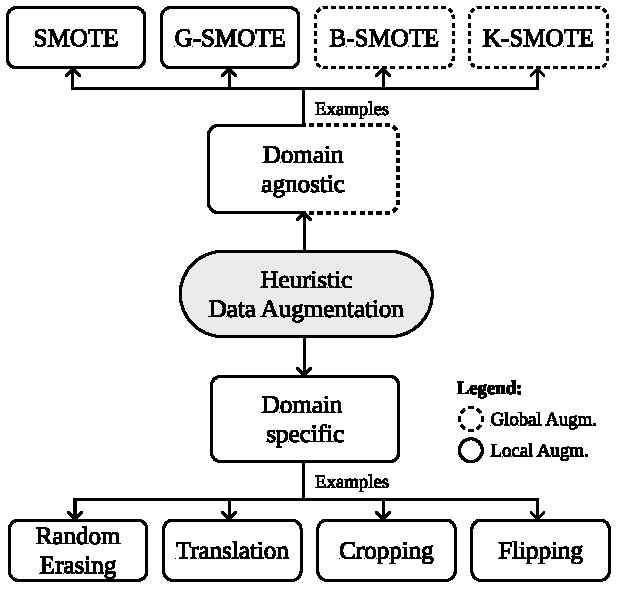
\includegraphics[width=.5\linewidth]{data_augmentation_taxonomy}
    \caption{%
        Schema containing a general Heuristic Data Augmentation taxonomy.
    }~\label{fig:data_augmentation_taxonomy}
\end{figure}

Heuristic approaches attempt to generate new and relevant observations through
the application a predefined procedure, usually incorporating some degree of
randomness~\cite{Kashefi2020}. Since these methods typically occur in the
input space, they require less data and computational power when compared to
Neural Network methods. Neural Network approaches, on the other hand, map the
original input space into a lower-dimensional representation, known as the
feature space~\cite{DeVries2017}. The generation of artificial data occurs in
the feature space and is reconstructed into the input space. Although these
methods allow the generation of less noisy data in high-dimensional contexts
and more plausible artificial data, they are significantly more
computationally intensive. Considering the scope of this thesis, the
computational power available for this experiment and the breadth of datasets
used in the different experimental procedures, we will focus on
domain-agnostic heuristic data augmentation methods.

While some techniques may depend on the domain, others are domain-agnostic.
For example, Random Erasing~\cite{Zhong2020}, Translation, Cropping and
Flipping are image data-specific augmentation methods. Other methods, such as
most of the variants of the Synthetic Minority Oversampling TEchnique
(SMOTE)~\cite{Chawla2002}, may be considered domain agnostic. However, SMOTE
methods were originally developed as oversamplers, whose goal is to balance
the class frequencies of the target variable in the training dataset and
address the class imbalance bias. Therefore, oversampling methods may be
considered a subset of Data Augmentation. Data Augmentation strategies may
follow varying augmentation strategies, which do not necessarily depend on
the target class distribution. An example of the differences among general
data augmentation and oversampling generation strategies is shown in
Figure~\ref{fig:augmentation_strategies}.

\begin{figure}[ht]
	\centering
	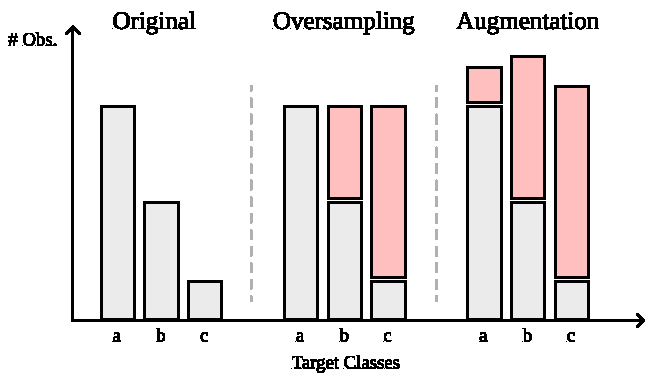
\includegraphics[width=.6\linewidth]{augmentation_strategies}
    \caption[Examples of data augmentation Strategies.]{%
        Examples of data augmentation Strategies. The salmon-colored bars
        represent artificial data using the normal oversampling (center group) and
        an example of augmentation (right group) strategies.
    }~\label{fig:augmentation_strategies}
\end{figure}

The simplest approach found in the literature is randomly duplicating existing
training observations. As a non-informed data generation method, although
simple to implement, it increases the risk of overfitting and generally
performs worse than other informed heuristic
methods~\cite{Douzas2019rs}.

The SMOTE method generates artificial data via the linear interpolation
between a random observation and one of its $k$-nearest neighbors (also
randomly selected)~\cite{Chawla2002}. Although simple and effective, it also
contains several limitations which motivated the development other variants,
discussed below. Specifically, its selection mechanism does not consider the
global structure of the dataset while its generation mechanism introduces
little variability into the training dataset~\cite{Douzas2019}.
Borderline-SMOTE (B-SMOTE)~\cite{Han2005} improves the selection mechanism by
attributing a larger importance to the observations closer to the decision
boundaries. The selected observations are used to run the SMOTE method in
order to produce better defined decision boundaries. A more recent improvement
of the selection mechanism is K-means SMOTE (K-SMOTE)~\cite{Douzas2018}. This
method uses a clustering-based approach to overcome imbalances between and
within classes, while considering the densities of each region of the input
space.

\begin{figure}[ht]
	\centering
	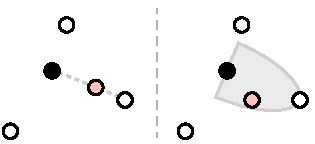
\includegraphics[width=.4\linewidth]{smote_vs_gsmote}
    \caption[Examples of data generation using SMOTE and G-SMOTE\@.]{%
        Examples of data generation using SMOTE and G-SMOTE\@. In this
        example, both G-SMOTE's deformation and truncation parameters assume
        values around $0.5$.
    }~\label{fig:smote_vs_gsmote}
\end{figure}

G-SMOTE~\cite{Douzas2019} modifies SMOTE's generation mechanism. Instead of
generating an observation as a linear combination between 2 others, it
generates observations within an hypersphere defined using the selected
observation as its center and one of its nearest neighbors as its boundary.
The hypersphere contains two hyperparameters, the truncation and deformation
factors, which limit the area of the hypersphere. The difference between SMOTE
and G-SMOTE is shown in Figure~\ref{fig:smote_vs_gsmote}.

\section{Active Learning}~\label{sec:active_learning}

Supervised ML algorithms typically perform well in contexts where labeled data
is abundant and accessible. However, in a practical setting, finding this data
is frequently a challenging task. Depending on the domain, collecting large
volumes of data may not be feasible since the labeling of such data becomes
labor and time intensive and may involve domain experts throughout the
process~\cite{Cao2020}. AL maximizes a classifier's performance while
annotating as least observations as possible. It assumes that observations
within the same dataset have a different contribution to the training of ML
classifiers~\cite{Ren2021}. Consequently, the data annotation cost can be
minimized via the annotation of the most valuable observations within an
unlabeled input space. The goal is to iteratively maximize the classification
performance of ML algorithms while minimizing the required amount of training
data to reach a certain performance threshold~\cite{Shrivastava2021}. It
allows the implementation of ML classifiers with a good performance and
minimal effort when compared to randomly selecting data or labeling the entire
unlabeled dataset~\cite{Ren2021}. Therefore, it addresses the labeling problem
in scenarios with a limited budget, time, or availability of labeled data. 

AL methods may be divided into 2 different stages, initialization and
iteration. Figure~\ref{fig:al_initialization} shows a diagram that represents
the typical AL initialization. Assuming the AL task is initialized without any
previously labeled data, it is typically composed of 3
steps~\cite{Fonseca2021}: 

\begin{enumerate}
    \item Collection of an unlabeled dataset, where the procedure depends on
        the domain of application.
    \item Selection of an initial data subset. Typically, when there is no a
        priori labeled dataset, the initial data subset is randomly picked
        from the unlabeled dataset.
    \item Data labeling. The supervisor is presented with the data subset,
        where its goal is to label each observation. Some of the research
        refers to the supervisor as the oracle~\cite{Yoo2019, Aghdam2019}.
\end{enumerate}

\begin{figure}[ht]
	\centering
	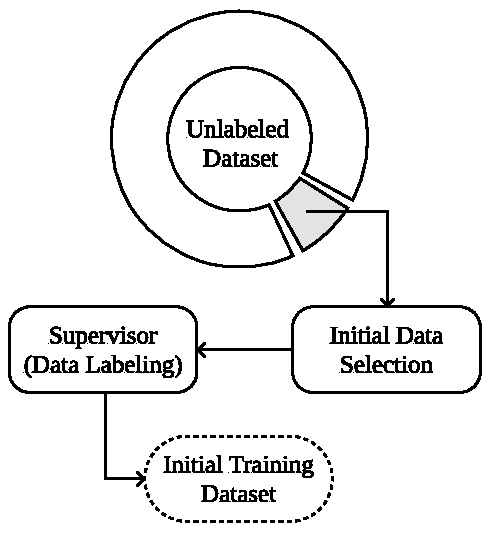
\includegraphics[width=.35\linewidth]{al_initialization}
    \caption{%
        Diagram depicting an AL initialization.
    }~\label{fig:al_initialization}
\end{figure}

Once an initial training dataset is set up, the iterative process of AL takes
place. An AL iteration is completed once a new batch of labeled data is added
to the training dataset. A standard AL process is shown in
Figure~\ref{fig:al_iteration_int} and is composed of the following
steps~\cite{Su2020, Sverchkov2017}:

\begin{enumerate}

    \item Setting up a classification algorithm and uncertainty criterion. The
        classifier is trained using the labeled dataset (\textit{i.e.,} the
        Current Training Dataset), and is used to predict the class membership
        probabilities of the observations found in the unlabeled dataset. The
        class probabilities are passed into an Uncertainty Criterion, which
        will return the classification uncertainty of the classification
        algorithm for each unlabeled observation. The combination of the
        classifier, along with the uncertainty criterion is sometimes referred
        to as the Query/Acquisition function~\cite{Rosario2020}.

    \item Selecting the top N observations. Since it is not possible to
        determine a priori whether the classifier's prediction is correct or
        not, the N observations with highest uncertainty may have been
        unknowingly correctly classified. However, regardless of the
        classification quality, these observations are expected to provide the
        most meaningful information to train the classifier in the next
        iteration.

    \item Labeling the selected N observations and updating the current
        training dataset with the new training observations. The selected
        observations from the unlabeled dataset are presented to the
        supervisor, which is responsible for manually labeling the
        observations. The new (labeled) training observations are added to the
        training dataset and the iteration is completed.

\end{enumerate}

\begin{figure}[ht]
	\centering
	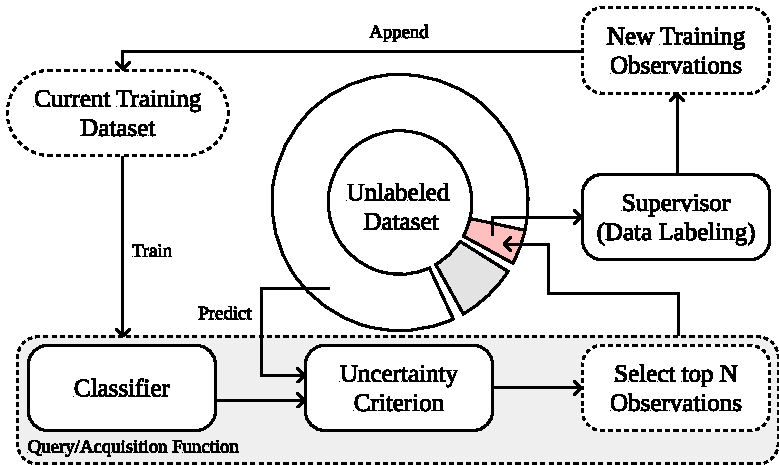
\includegraphics[width=.6\linewidth]{al_iteration}
    \caption[Diagram depicting an AL iteration.]{%
        Diagram depicting an AL iteration. In the first iteration, the
        training set collected during the initialization process becomes the
        ``Current Training Dataset''.
    }~\label{fig:al_iteration_int}
\end{figure}

Two common challenges found in AL implementations are the consistency and
efficiency of AL in practical scenarios~\cite{Kottke2017}. On the one hand,
the consistency problem refers to the high variance in performance (regarding
classification and data selection) over different initializations
(\textit{i.e.,} different initial training datasets) of active learners. On
the other hand, the efficiency problem refers to the maximization of the
quality of the collected data over a run. Therefore, a good active learner is
capable of having a consistent performance over different initializations
while ensuring the production of high-performing classifiers with the least
possible amount of data. There are various factors that may affect the
consistency and efficiency of the AL framework: (1) Human error during data
labeling~\cite{li2020}, (2) Non-informative initial training
dataset~\cite{Nguyen2004} and (3) Lack of an appropriate uncertainty
criterion~\cite{Rosario2020}. AL research has typically been focused on the
specification of uncertainty criteria, as well as domain-specific
applications. Query functions can be divided into two different
categories~\cite{Gu2021, Kumar2020}: 

\begin{enumerate}

    \item Informative-based query strategies. These strategies use the
        classifier's output to assess the importance of each observation
        towards the performance of the classifier. These strategies focus on
        quantifying the class uncertainty of the unlabeled observations.
        Since these techniques do not account for the relationships between
        the unlabeled observations and treats each observation
        independently~\cite{Fu2013}.

    \item Representative-based query strategies. These strategies estimate the
        optimal set of observations that will optimize the classifier's
        performance. This strategy contains 3 main approaches: Density-based,
        Diversity-based and Exploration of graph structures. Although this
        method addresses the problem of sampling bias and redundant instance
        selection, these strategies typically require more observations in
        order to reach the desired classification
        performance~\cite{Kumar2020}.

\end{enumerate}

Although there are significant contributions towards the development of more
robust query functions and classifiers in AL, modifications to AL's basic
structure are rarely explored. In~\cite{Yoo2019} the authors introduce a loss
prediction module in the AL framework to replace the uncertainty criterion.
This model implements a second classifier to predict the expected loss of the
unlabeled observations (using the actual losses collected during the training
of the original classifier) and return the unlabeled observations with the
highest expected loss. Although this contribution is specific to neural
networks (and more specifically, to deep neural networks), they were able to
significantly improve the efficiency of data selection in AL\@.
In~\cite{Simeoni2020} the authors propose the usage of semi-supervised
learning during both the initialization of the AL and the iterative process as
well. However, this method was proposed specifically for deep learning
applications.

A query strategy/function encompasses all the steps prior to the data labeling
within an AL iteration. They focus on finding the observations'
informativeness, representativeness or both~\cite{Gu2021, Kumar2020}.
Representative query strategies are generally less efficient in data selection
than Informative query strategies~\cite{Kumar2020}. However, recent research
often use representative approaches alongside informative
approaches~\cite{Gu2021, Samat2016}. Representative query strategies are
explored via 3 main approaches~\cite{Kumar2020}: 

\begin{enumerate}
    \item Density-based, which select representative observations from high
        density regions.~\cite{Huang2014, Li2012, Ienco2013} used a
        density-based approach using clustering algorithms to select the
        observations closest to the centroid of each cluster. 
    \item Diversity-based, which select the N observations at each iteration
        that maximize the diversity in the training data. The diversity-based
        approach was developed to avoid the selection of redundant
        observations in batch-mode learning~\cite{Brinker2003}.
    \item Graph-based, which find the most representative nodes and edges of a
        graph network~\cite{Jia2019}. Since these methods are specific to
        graph network data, they have a more limited applicability.
\end{enumerate}

Informative query strategies, unlike representative query strategies, do not
account for the structure of the unlabeled dataset. As a result, this type of
strategy may lead to the inefficient selection of observations (\textit{i.e.,}
redundant observations with similar profiles)~\cite{Kumar2020}. Research on
more robust selection criteria attempts to address the efficiency problem.
This is motivated by the importance of the selection criteria in AL's
iterative process~\cite{Rosario2020}. Specifically, Settles~\cite{Settles2011}
observed that in some datasets informative query strategies fail to outperform
the random selection of observations. Generally, the Random Selection query
method is used as a baseline. This method disregards the class membership
probabilities produced by the classifier and returns N random points from the
dataset without following any specific criteria.

A frequently used query strategy is Uncertainty Sampling, originally proposed
in~\cite{Lewis1994}. Using this method, the estimation of an observation's
uncertainty is based on the target class with the highest probability ($p_a$,
according to the classifier) and the uncertainty is calculated as $1-p_a$.
However, since this method dismissed the classifier's predictions on the
remaining labels, the Breaking Ties criterion was proposed to address this
limitation for multiclass problems~\cite{Luo2005}. This method uses the two
target classes with highest probability ($p_a$ and $p_b$, according to the
classifier) and the uncertainty is calculated as $p_a - p_b$ (in this case,
the lower the output value, the higher the uncertainty). Recent variants of
the Breaking Ties criterion, such as the Modified Breaking Ties, attempted to
fix some limitations of the original method~\cite{Liu2018, Li2012a}.

Another common informative query strategy is the calculation of Shannon's
Entropy. This metric measures the level of uncertainty
based on the probabilities of a set of possible events. Its formula is given
by $H(p)=-\sum_{i=0}^n{p_i\log_2{p_i}}$, having $p$ as the set of
probabilities of all target classes. The application of the Entropy
uncertainty criterion is also frequently applied in Deep Active
Learning~\cite{Aghdam2019}. Other Entropy-based methods were also developed
for more specific applications. For example, an ensemble querying approach
known as Entropy Querying-by-Bagging uses the predictions of all estimators to
find the maximum entropy of each observation~\cite{Abe1998}.

The Query by Committee (QBC) strategy was developed to address ensemble
classifiers. It is a disagreement based strategy that attempts to maximize the
information gain at each iteration by computing the disagreement of the
predictions over the estimators that form the ensemble. The Entropy
Querying-by-Bagging and Query-by-Boosting methods are also ensemble
strategies. Query by boosting and bagging methods were found to achieve a good
performance over various datasets~\cite{Melville2004}, while the performance
between the two strategies appears to differ significantly across various
scenarios~\cite{Bloodgood2018}.

Other classifier-specific query strategies were also developed for different
applications. However, these methods have the disadvantage of depending on the
classifier being used. For example, Margin Sampling is a well studied strategy
that uses a Support Vector Machine as its classifier in order to select the
unlabeled observations closest to its decision boundaries~\cite{Kumar2020}.
Although, since this method is known to lead to the excessive selection of
observations in dense regions~\cite{Zhou2014}, it was improved in various
ways. In~\cite{Zhou2014} the authors extend this strategy by applying the
manifold-preserving graph reduction algorithm beyond the normal Margin
Sampling method.


\section{Research Questions}

This dissertation aims to explore and develop new domain-agnostic methods,
leveraged by synthetic data generation techniques, while showing their
effectiveness in difficult classification problems, specifically LULC
classification. The main research questions (RQ) and goals of this
dissertation are the following:

\begin{enumerate}
    \item What are the main research lines in synthetic data generation?
          \begin{itemize}
              \item Development of a literature review to study existing
                  synthetic data generation methods and the core fields where
                  they are being used.
          \end{itemize}
    \item How can one oversample data with both continuous and categorical
        features? 
        \begin{itemize}
            \item Development of an improved oversampling method to be used
                with mixed data types.
        \end{itemize}
    \item How can the quality and consistency of automatic LULC mapping be
        enhanced?
          \begin{itemize}
              \item Exploration of imbalanced learning methods in the context
                  of LULC\@.
          \end{itemize}
    \item How can efficient automated LULC mapping be achieved with limited
        availability of ground-truth data?
        \begin{itemize}
            \item Development of an improved active learning framework in the
                remote sensing domain using artificial data generation.
        \end{itemize}
\end{enumerate}

\section{Main Objectives}~\label{sec:main_objectives}

This research aims to apply and develop new data preprocessing techniques to
LULC classification, with a focus on AL and oversampling techniques. The main
objective is to optimize ML classifiers' performance with minimal labeled data
and/or imbalanced learning scenarios. This objective was decomposed into four
research questions. We start by performing a literature review of synthetic
data generation techniques (RQ1). Second, we propose a new oversampling method
for datasets with both continuous and categorical features (RQ2). Third, we
apply a state-of-the-art oversampling method to understand its effect in LULC
classification tasks (RQ3). Finally, we modify the AL framework to include a
generator and optimize its augmentation policy to reduce the amount of labeled
data required for ML classifiers to reach a satisfactory performance (RQ4).

Each contribution towards the different RQs is divided into different studies.
All chapters refer to a different RQ with the exception
Chapters~\ref{chp:al-generator-lulc}
and~\ref{chp:active-learning-augmentation}, which refer to RQ3. The structure
of this dissertation is shown in Table~\ref{tab:studies}.

RQ1 aims to investigate and consolidate data augmentation methods. This was
done by conducting a literature review to understand the main areas of
application of synthetic data generation and identify the generation
mechanisms available for this purpose. To do this, we conducted an extensive
literature search, compiled the knowledge collected in related literature
reviews, and analyzed several data generation techniques and areas of
application. This approach resulted in a compilation of the most important and
current research in the field, allowing both researchers and practitioners to
use this work as a starting point for their own work. Finally, the development
of this work represents a crucial step to identify new opportunities within
the field and addressing the remaining research questions. The results of this
work is available in Chapter~\ref{chp:synthetic-data-review}.

One of the main limitations uncovered in RQ1 (see
Chapter~\ref{chp:synthetic-data-review}) is the lack of oversampling
methods applicable to datasets containing categorical features. In fact, only
two oversamplers were found to be well-suited for oversampling data with mixed
data types, SMOTENC~\cite{Chawla2002} and random oversampling.  However, in a
practical setting, datasets with mixed feature types are common but the
methods available are outdated. RQ2 is addressed with the modification of a
state-of-the-art oversampling method by mixing its data generation mechanism
with the one found in SMOTENC\@.

Several relevant methods found in Chapter~\ref{chp:synthetic-data-review}
will be used for posterior work. Specifically, we address RQ3 using a
heuristic data augmentation method, K-means SMOTE~\cite{Douzas2018}, as
described in Chapter~\ref{chp:kmeans-smote}. Since datasets produced for LULC
classification often contain irrelevant, redundant, noisy and/or unreliable
data, knowledge discovery is hindered and ultimately leads to the poor
training of predictors. Consequently, data preprocessing becomes an important
contribution to the quality of the predictors developed. In this case, we used
K-means SMOTE to oversample minority regions belonging to the same land cover
class. This was motivated by the challenges faced in producing automated LULC
maps using a training dataset with rare classes. In this scenario, the
spectral signature of a given class often depends on its geographical
distribution and the time of the year the image was captured. Cluster-based
oversamplers, such as K-means SMOTE, allow for a more accurate generation of
minority samples, since it can identify and isolate variations in spectral
signatures within a land cover class.

At a later stage, in RQ4, we addressed a different instance of the problem of
rare land cover classes in the training dataset. Specifically, in a context of
limited sample-collection budget, the collection of the most informative
samples capable of optimally increasing the classification accuracy of a LULC
map is of particular interest~\cite{Su2020}. Active learning attempts to
minimize the human-computer interaction involved in photo-interpretation by
selecting the data points to include into the annotation process. Although,
current state-of-the-art techniques are mostly focused on the improvement of
the acquisition function. We study this problem via the modification of the
typical AL framework. We focus on the usage of data augmentation techniques
and an augmentation policy optimizer to improve the quality of the data
generated. These modifications are presented in
Chapters~\ref{chp:al-generator-lulc}
and~\ref{chp:active-learning-augmentation}:

\begin{itemize}
    \item Chapter~\ref{chp:al-generator-lulc} introduces the generator
        component into the typical AL framework.
    \item Chapter~\ref{chp:active-learning-augmentation} introduces the
        augmentation policy optimizer, while generalizing the generator
        component for augmentation policies beyond oversampling strategies.
\end{itemize}

\section{Methods}

The methodology used for all contributions follows a similar approach, with
exception to the work presented in Chapter~\ref{chp:synthetic-data-review}.
It is composed as follows:

\begin{enumerate}
    \item Collection of a large number of (LULC or multidisciplinary)
        classification datasets.
    \item Identification of related literature and limitations to be addressed.
    \item Design and implementation of contributions.
    \item Definition and implementation of experimental settings.
    \item Analysis of results and statistical significance testing.
    \item Publish results.
\end{enumerate}

The methodological approach to the proposed doctoral work is depicted in
Figure~\ref{fig:phd_structure}. All of the work presented was developed while
ensuring full reproducibility. Contributions at the algorithm-level are
implemented in the Python open-source package 
\href{https://github.com/joaopfonseca/ml-research}{ML-Research}. At the time
of writing, the ML-Research package has been downloaded 12 thousand times via
the Python Package Index (pypi/pip) and Anaconda (conda-forge channel).

\begin{figure}[ht]
	\centering
    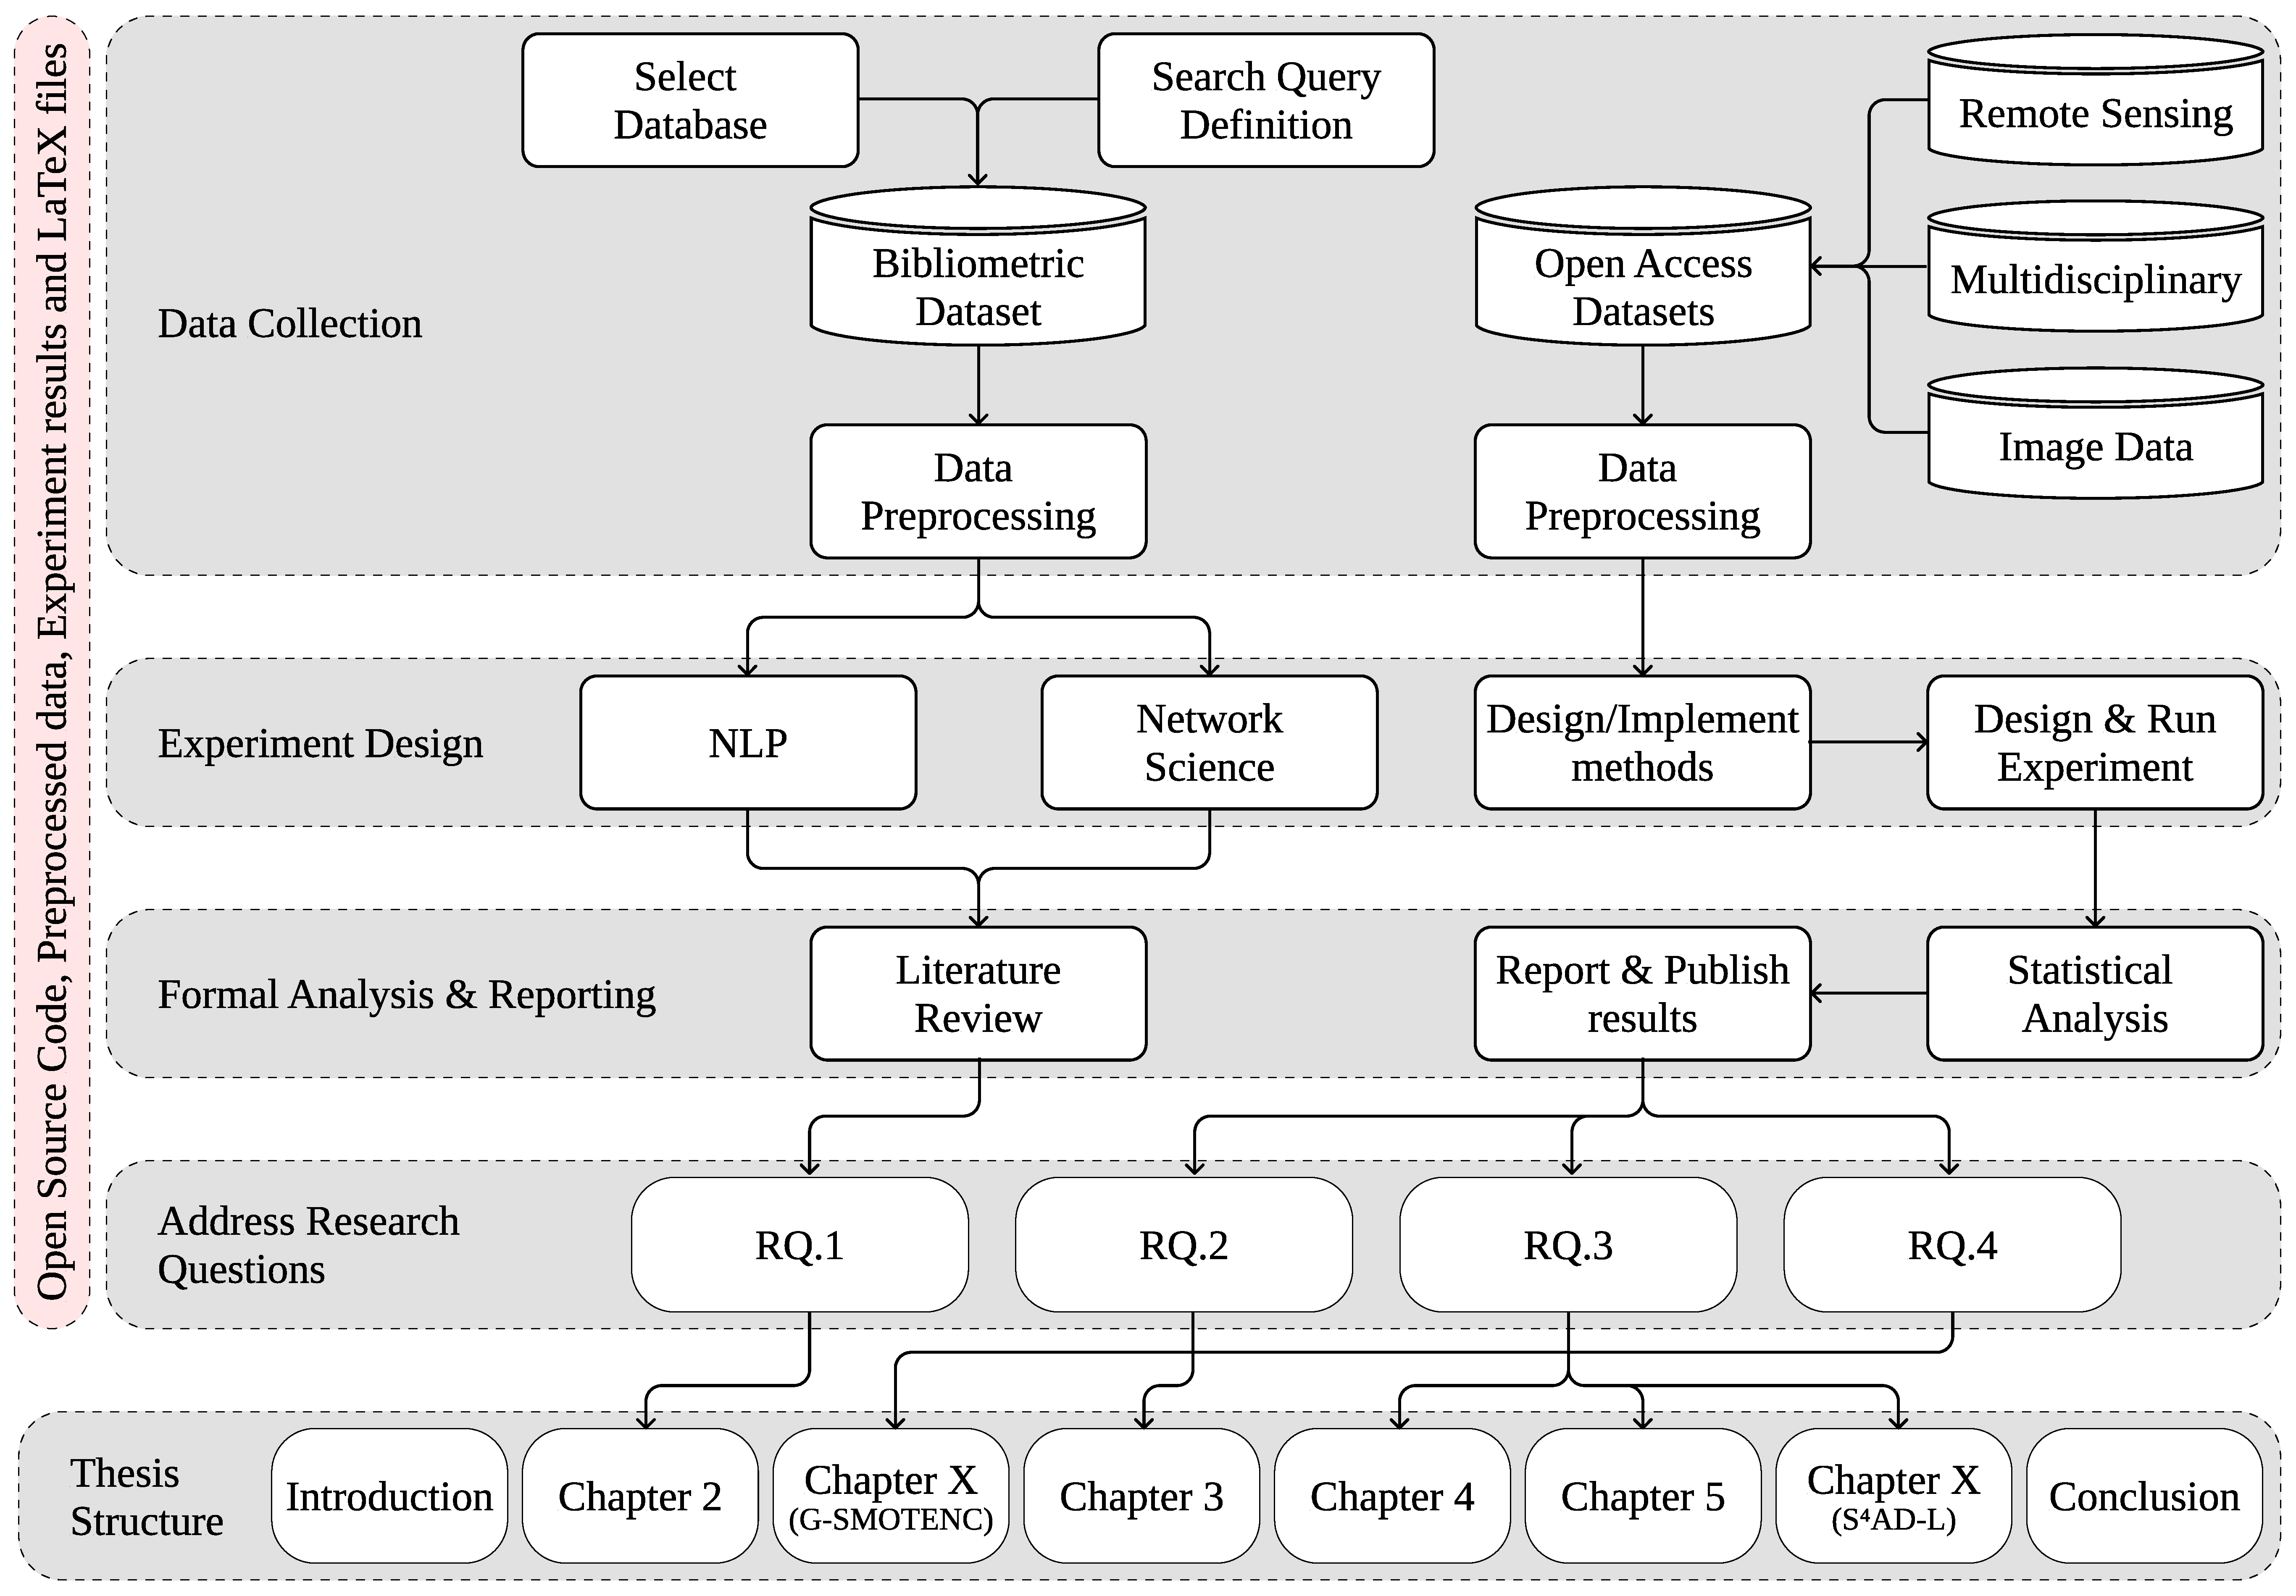
\includegraphics[width=\linewidth]{phd_structure}
    \caption{Structure and methodological approach used in this dissertation.
    }~\label{fig:phd_structure}
\end{figure}


\section{Path of Research}

Each chapter corresponds to a paper (either published or under submission),
all of which primarily focused on AL and imbalanced learning, with exception
to Chapter~\ref{chp:synthetic-data-review}. All of these research outputs are
available at \href{https://github.com/joaopfonseca/publications}{this GitHub
repository}, along with the \LaTeX\ scripts, data, source code (for data
pulling, preprocessing, experiments and analysis), experiments' raw outputs
and analysis outputs (figures, tables and diagrams). The current stage of the
studies is presented in Table~\ref{tab:studies}.

\begin{table}%[ht]
    \centering
    \begin{tabular}{ccm{.55\textwidth}m{.2\textwidth}}
        \toprule
        Chapter & RQ & Study Name                                                        & Current stage  \\
        \midrule
        \ref{chp:synthetic-data-review} & 1    & Tabular and Latent Space
                                                 Synthetic Data Generation: 
                                                 A Literature Review                      & Under Review   \\
        % Research Trends and Applications 
        %                                            of Data Augmentation
        %                                            Algorithms                          & Under Review 
        %                                                                            (Initial submission)  \\
        \vspace{-.2cm}\\
        \ref{chp:gsmotenc} & 2     & Geometric SMOTENC\@: A geometrically
                                     enhanced drop-in replacement for SMOTENC          & Under Review    \\
        \vspace{-.2cm}\\
        \ref{chp:kmeans-smote}             & 3    & Improving Imbalanced Land Cover 
                                                   Classification with K-means SMOTE: 
                                                   Detecting and Oversampling 
                                                   Distinctive Minority Spectral 
                                                   Signatures                          & Published in 
                                                                                         the journal 
                                                                                         Information      \\
        \vspace{-.2cm}\\
        \ref{chp:al-generator-lulc}        & 4    & Increasing the Effectiveness of 
                                                   Active Learning: Introducing
                                                   Artificial Data Generation in 
                                                   Active Learning for Land Use/Land 
                                                   Cover Classification                & Published in 
                                                                                         the journal 
                                                                                         Remote Sensing   \\
        \vspace{-.2cm}\\
        \ref{chp:active-learning-augmentation} & 4 & Improving Active Learning 
                                                   Performance Through the Use of
                                                   Data Augmentation
                                               & Published in International
                                               Journal of Intelligent Systems   \\
        \bottomrule
    \end{tabular}
    \caption{\label{tab:studies}
        Publication stage of the studies developed in the scope of the doctoral
        program.
    }
\end{table}

This dissertation uses synthetic data generation as the core concept
throughout its development. The contributions presented in each chapter
can be split between domain specificity (agnostic versus LULC-specific) and
base technique (oversampling versus AL).
Chapter~\ref{chp:synthetic-data-review} presents a comprehensive literature
review of the central concept of the dissertation, synthetic data generation.
Chapter~\ref{chp:gsmotenc} proposes a domain-agnostic oversampling technique,
to address the problem of datasets with mixed data types (\textit{i.e.},
containing both metric and non-metric features).
Chapter~\ref{chp:kmeans-smote} applies an oversampling technique to LULC
classification problems. Chapter~\ref{chp:al-generator-lulc} proposes an AL
framework using synthetic data generation applied to LULC classification.
Section~\ref{chp:active-learning-augmentation} modifies and improves the
AL framework proposed in the previous chapter and ensure its effectiveness
over several different domains. 

\thesischapter{%
    Research Trends and Applications of Data Augmentation Algorithms
}{%
    Submitted as Joao Fonseca, Fernando Bacao, to a Q1 Journal, 2022
}~\label{chp:data-augmentation-trends}
\graphicspath{{figures/data-augmentation-trends/}}

\begin{adjustwidth}{30pt}{30pt}

    In the Machine Learning research community, there is a consensus regarding
    the relationship between model complexity and the required amount of data
    and computation power. In real world applications, these computational
    requirements are not always available, motivating research on
    regularization methods. In addition, current and past research have shown
    that simpler classification algorithms can reach state-of-the-art
    performance on computer vision tasks given a robust method to artificially
    augment the training dataset. Because of this, data augmentation
    techniques became a popular research topic in recent years. However,
    existing data augmentation methods are generally less transferable than
    other regularization methods. In this paper we identify the main areas of
    application of data augmentation algorithms, the types of algorithms used,
    significant research trends, their progression over time and research gaps
    in data augmentation literature. To do this, the related literature was
    collected through the Scopus database. Its analysis was done following
    network science, text mining and exploratory analysis approaches. We
    expect readers to understand the potential of data augmentation, as well
    as identify future research directions and open questions within data
    augmentation research.

\end{adjustwidth}

\vspace{.5cm}
\textbf{Keywords:} Data Augmentation; Generative Adversarial Networks; Regularization
Methods; Overfitting

\section{Introduction}~\label{sec:introduction-aug}

The performance of Machine Learning models is highly dependent on the quality
of the training dataset used~\cite{Fenza2021, Halevy2009}. Specifically, the
presence of imbalanced and/or small datasets, target labels incorrectly
assigned, outliers and high dimensional input spaces reduce the prospects of a
successful machine learning model implementation~\cite{Halevy2009,
Domingos2012, Salman2019}.  Even though the performance of any classifier is
affected by the size of its training dataset, deep learning models have a
particularly inconsistent performance over unseen datasets even when trained
with large datasets~\cite{Hu2020, Xie2021}.  Conversely, deep learning models
are capable of quickly adapting (and overfitting) to the training dataset,
including when it contains label and/or complete pixel noise~\cite{Xie2021,
Zhang2021}.  Although the performance of these models can be improved through
regularization methods, they are still incapable of correcting label noise in
the training dataset~\cite{Zhang2021}.

Regardless of the machine learning model used, when the training set contains
significant limitations (regarding overall quality and size), the model's
performance on unseen data is generally going to be affected. Specifically,
when the training data is not representative of the true population, or the
model is over-parametrized, it becomes particularly prone to
overfitting~\cite{Bartlett2021}. There are different strategies to reduce
overfitting, known as regularization methods~\cite{Shorten2019}. Identifying
the appropriate regularization methods varies according to the use
case~\cite{Chun2020}. While some methods can only be applied on specific
classifiers, data types or domains, others may be applied at the data level,
independently from the classification problem. For example, methods such as
dropout/dilution, batch normalization and transfer learning/domain adaptation
are mostly applied on neural network architectures.  Pruning is applied on
decision trees. Early stopping can be used on learners trained iteratively,
making it a broader method. 

Data augmentation techniques are used to increase the size (and hopefully the
diversity) of data in a training dataset through the production of artificial
observations~\cite{Van2001, Wong2016}. They are frequently used as
regularization techniques for various types of problems and classifiers, since
it is applied at the data level~\cite{Behpour2019}.
Figure~\ref{fig:data_augmentation_example} shows an example of data
augmentation, where the decision boundaries become clearer after the original
dataset is augmented. Data Augmentation methods can be divided into heuristic
and Deep Learning approaches~\cite{Shorten2019, Ratner2017}. Within these
approaches, they may be either domain specific or contextually independent.
For example, although both Synthetic Minority Oversampling Technique
(SMOTE)~\cite{Chawla2002} and Kernel Filters are heuristic approaches, SMOTE
may be used regardless of the context, while Kernel Filters are specific to
image data augmentation. The different types of Data Augmentation methods are
defined at a higher detail in Section~\ref{sec:data-augmentation-aug}.

\begin{figure}
	\centering
	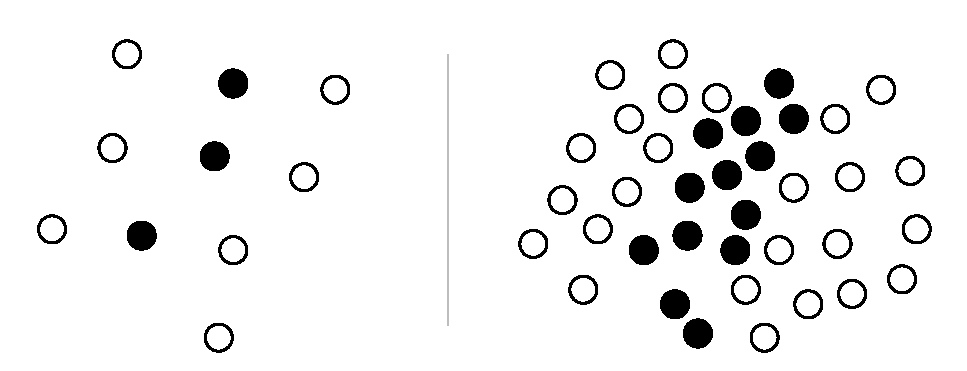
\includegraphics[width=.9\linewidth]{data_augmentation_example}
    \caption[Example of data augmentation in a 2-dimensional binary
    classification setting.]{Example of data augmentation in a 2-dimensional
        binary classification setting. The left pane contains the original
        dataset, where the amount data is scarce and the gap among the two
        classes are wide, allowing for greater classification variability. The
        right pane contains the augmented dataset, where the gap among the two
        classes is narrower and the decision boundaries become easier to
        define.
    }~\label{fig:data_augmentation_example}
\end{figure}

In 2011, Jürgen Schmidhuber's group showed that a MLP ensemble architecture
can achieve state-of-the-art performance on computer vision benchmarks given
strong enough data augmentation~\cite{Meier2011, Ciresan2011}. Although the
state-of-the-art improved since then, two recent papers developed by Google
Brain and Facebook research teams support Schmidhuber's group's findings.
Specifically, in~\cite{Tolstikhin2021, Touvron2021} the authors discuss two
similar MLP ensemble architectures, showing that the proposed model attains a
comparable performance to convolutional neural networks and attention-based
networks. Another recent study also discusses a related MLP architecture with
similar findings, while suggesting that the strong performance of computer
vision models may be attributable mainly to the inducive bias produced by the
patch embedding and the carefully-curated set of training
augmentations~\cite{Melaskyriazi2021}.

Research on data augmentation methods gained significant popularity in recent
years. As such, there were some efforts in the past to establish a taxonomy
and distinction of the different types of data augmentations
methods~\cite{Shorten2019}. To the best of our knowledge, there is no analysis
on data augmentation research as a whole, as well as domains of application
and future directions. In this paper we focus on current and past research
trends of data augmentation methods, its different applications and use cases.
This is done with an extensive analysis of the title, keywords and abstract of
a large set of literature related to data augmentation, collected through the
\href{https://www.scopus.com/}{Scopus} database using Natural Language
Processing and Network Science techniques. The analysis contains 3 phases. We
started by performing an exploratory data analysis to identify the most
significant publications, journals and conferences within the field of data
augmentation. Then, we analysed the articles' author keywords by constructing
a network and extracting and identifying communities of keywords.  Finally we
used a text mining approach to extract additional applications and methods
using the articles' abstracts, as well as validate the findings discussed with
the keyword analysis.

The rest of this paper is structured as follows:
Section~\ref{sec:data-augmentation-aug} describes the main methods and approaches
used in data augmentation, Section~\ref{sec:methodology-aug} describes the
procedures defined throughout the different analyses.
Section~\ref{sec:results_discussion-aug} presents and discusses the findings drawn
from the analyses, as well as research gaps and open questions in data
augmentation research. Section~\ref{sec:conclusion-aug} summarizes the main
findings discussed throughout the study.

\section{Data Augmentation Methods}~\label{sec:data-augmentation-aug}
 
Based on the literature found, a Data Augmentation method may be characterized
based on 3 criteria. The more common division is done between Heuristic and
Deep Learning approaches~\cite{Shorten2019}. Within these, several approaches
have been developed to produce artificial observations at the
input~\cite{Zhong2020}, feature~\cite{DeVries2017}, or output
space~\cite{Behpour2019}. Finally, we also distinguish them based on whether
their generation mechanism considers local (\textit{i.e.,} considers
partial/specific information within the dataset) or global (\textit{i.e.,}
it's based on the overall distribution/structure of the dataset) information
of the original dataset. Figure~\ref{fig:concept_map} depicts the concept map
with the different subdivisions of characteristics of data augmentation
methods. In this section, the analysis of the different types of data
augmentation will be based on their architectural approach. However, all the
methods mentioned may be divided using any of the definitions mentioned.

\begin{figure}[htb]
	\centering
	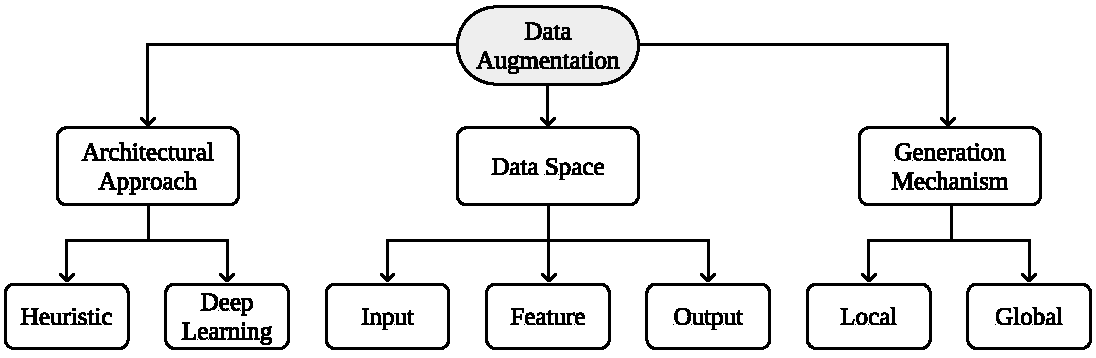
\includegraphics[width=\linewidth]{concept_map}
    \caption{%
        Data Augmentation concept map.
    }~\label{fig:concept_map}
\end{figure}

Heuristic methods use the information found in the input space to generate
new, relevant, non-duplicated observations by applying a predefined set of
rules, while incorporating a degree of randomness in the generation process.
Since data augmentation occurs in the input space, these are cost-effective
approaches to data augmentation. For this reason, heuristic methods are
simpler to implement and are particularly appealing for low dimensional
classification problems, especially when the computational power available is
limited. 

Some Deep Learning methods, on the other hand, attempt to map the original
input space into a lower-dimensional representation, known as feature
space~\cite{DeVries2017}. The generation of artificial observations occurs at
the feature space level, before being reconstructed to the original input
space. This is commonly done with Convolutional Neural Networks (CNN) and
auto-encoder architectures~\cite{Shorten2019}. Since data augmentation is
performed in the feature space, this type of approach is particularly useful
for high-dimensional data types and results in more plausible synthetic
observations~\cite{DeVries2017}. However, deep learning approaches require
more computational power than heuristic approaches and the resulting feature
space is difficult to interpret.

The difference in classification performance of the two perspectives is still
unclear. Wen et al.~\cite{Wen2020} evaluate the impact of data augmentation on
time series for various classification and forecasting tasks. Although they
found that both heuristic and deep learning approaches improved the results
over the various experiments, there was no direct comparison among the
different methods. Wong et al.~\cite{Wong2016} compared both input and feature
space data augmentation methods for image data classification performance over
the MNIST dataset. They found that input space augmentation can lead to better
classification performance if plausible transforms on the data are known.
However, in~\cite{DeVries2017} the authors discuss that the effectiveness of
each data augmentation method generally depends on the domain. The lack of
research on effective, domain-agnostic data augmentation methods appears to be
a current research gap.

\subsection{Heuristic Approaches}

Various heuristic approaches depend on the data type. For example, image data
augmentation may be done via translation, cropping or random
erasing~\cite{Zhong2020}, among others~\cite{Shorten2019}. However, these
techniques depend on the context and may not be applicable to other data types
such as time-series~\cite{Wen2020, Iwana2021} or tabular data. In this
subsection we will focus on domain-agnostic data augmentation methods.

Heuristic approaches may be applied at the input or feature space. The
appropriate method to be applied also depends on the machine learning goal.
Specifically, heuristic methods are commonly used to address classification
problems where the frequency of the different target classes vary
significantly, a problem known as Imbalanced Learning~\cite{Chawla2004}. In
this context, the dataset contains one or multiple rare classes, which become
more difficult to predict. This happens because during the learning phase,
classifiers are trained in order to maximize one or few performance metrics.
Although, a poor choice of performance metrics (\textit{i.e.}, a metric
insensitive to class imbalance, such as overall accuracy) might lead to a poor
estimation of the model's actual performance, since minority classes
contribute less to the learning phase and to the estimation of the performance
metric~\cite{Fonseca2021}. 

The problem of Imbalanced Learning is frequently addressed with oversampling
algorithms~\cite{Kaur2019}. Oversampling methods generate artificial
observations in order to balance class distributions using contextual
information based on the original dataset. These methods apply linear or
geometric interpolations between a random observation and one of its neighbors
to generate a new observation.

SMOTE~\cite{Chawla2002} is one of the most popular oversampling methods. It
generates an artificial observation along a line segment between a randomly
selected minority class observation and one of its nearest-neighbors. Since it
was first proposed, modifications at the neighbors parent observations
selection and data generation mechanisms of the original algorithm were
proposed. Borderline-SMOTE~\cite{Han2005} is an example of a modification of
SMOTE's data selection mechanism. Instead of selecting any random minority
class observation and one of its neighbors, the algorithm focuses in the
minority class observations closest to the decision boundary.
Geometric-SMOTE~\cite{Douzas2019} proposes a modification of the data
generation mechanism. Instead of generating data within a line segment, it
generates data within a hyper-spheroid between two parent observations.

Contrary to Deep Learning approaches, heuristic approaches can be applied at
the input space without the need of learning a feature space. This allows the
implementation of heuristic data augmentation with less computational power
and technical complexity. In addition, in contexts of limited data
availability (\textit{i.e.}, small datasets), deep learning approaches are not
appropriate since the amount of parameters to be tuned during the learning
phase often exceeds the number of observations in the dataset, making it
over-parametrized. The augmentation of small datasets using heuristic
approaches is explored in an Active Learning context
in~\cite{Fonseca2021al}. The authors found that significantly smaller
amounts of curated data using Active Learning, along with heuristic data
augmentation methods, achieved a classification performance comparable to
classifiers trained over the full dataset.

\subsection{Deep Learning Approaches}

Different deep learning approaches and architectures have been developed for
various domains. Deep learning data augmentation methods may be developed via
augmentation at the feature space (which involves learning a feature
space)~\cite{DeVries2017} or via a combination of a set number of observations
into a neural network in order to output a non-linear, non-geometric
combination of input observations~\cite{Wang2017}. Other domain-specific deep
learning methods also exist, such as style transferring techniques (specific
to image data)~\cite{Wang2017, Zhu2017}.

Data augmentation at the feature space is especially useful when dealing with
high-dimensional datasets with complex and/or discontinuous distributions.
For example, many heuristic data augmentation techniques cannot be applied in
handwritten digits classification problems since they may change the true
label of the generated image and generate noisy data. In this situation,
performing data augmentation at the input space may introduce
noise~\cite{Chu2020}, since the data is also subjected to the curse of
dimensionality (see Figure~\ref{fig:input_vs_feature_space}a). This allows
transformations of known observations in a lower dimensional space to generate
new, non-noisy artificial observations projected in the input space, as shown
in Figures~\ref{fig:input_vs_feature_space}b
and~\ref{fig:input_vs_feature_space}c. 

\begin{figure}[htb]
	\centering
	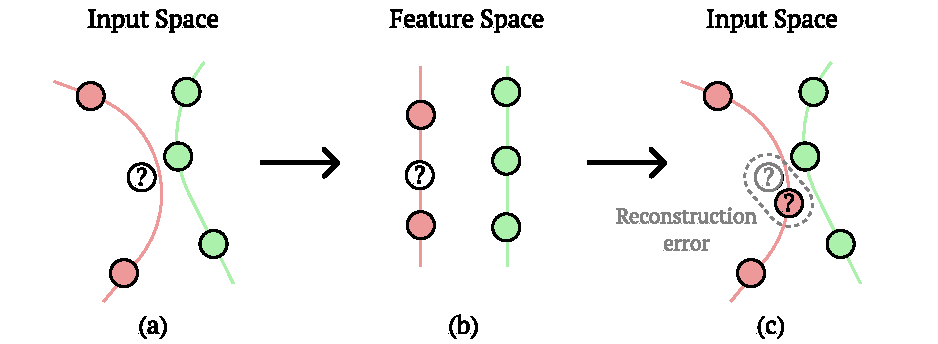
\includegraphics[width=.9\linewidth]{input_vs_feature_space}
    \caption[Example of a sparse input space and its corresponding feature
    space.]{%
        Example of a sparse input space and its corresponding feature space.
        Learning a manifold feature space facilitates the generation of
        non-noisy artificial data. In the original input space (a) the
        unseen/artificial observation marked with ``?'' is closer to a green
        observation and to the learnt red manifold space, which may lead to a
        noisy observation. When projected or generated in the feature space
        (b), the observation will better match the nearest manifold measure
        and avoid noisy data in the input space (c). Adapted
        from~\cite{Antoniou2017}.
    }~\label{fig:input_vs_feature_space}
\end{figure}

The utilization of autoencoders~\cite{Kramer1991} is particularly useful to
perform feature space data augmentation~\cite{Shorten2019}. Autoencoders are
composed by an encoder and a decoder, which map the input space to and from
the feature space, respectively. The autoencoder is trained by minimizing the
difference between the original observation and the reconstructed observation
(see Figure~\ref{fig:input_vs_feature_space}c). Once the training phase is
completed, heuristic methods are applied in the feature
space~\cite{DeVries2017}.

Generative Adversarial Network (GAN)~\cite{Goodfellow2014} architectures is a
deep learning approach frequently used as a data augmentation method. It
involves a generator and a discriminator. Although many different
architectures have been proposed, the generator in the vanilla GAN algorithm
may be seen as a decoder, which is trained based on the gradients calculated
via the discriminator. The discriminator attempts to distinguish true and
generated (fake) observations in order to assess the quality of the data
produced by the generator. The problem is better formulated as a minimax
decision rule, where the generator attempts to fool the discriminator by
producing observations that are difficult to classify as generated.

When the size of the training dataset is not sufficiently large to employ deep
learning approaches and other related datasets or unlabeled datasets are
available, one technique that may also be used is transfer learning. In this
context, the data augmentation model is trained on a secondary model and is
later adjusted to the training dataset. This allows the usage of deep learning
models in few-shot learning environments~\cite{Antoniou2017}.

\section{Methodology}~\label{sec:methodology-aug}

In this section we describe the procedures defined for the literature
collection, data preprocessing and literature analysis. The analysis of the
literature was developed with 3 different approaches. Throughout the
analyses, data preprocessing and hyperparameter tuning was developed
iteratively. The procedure adopted in this manuscript is shown in
Figure~\ref{fig:slr_diagram}.

The literature collection procedure is described in
Subsection~\ref{sec:lit_collection-aug}. The data and text preprocessing is
described in Subsection~\ref{sec:data_preprocessing-aug}. The exploratory data
analysis described in Subsection~\ref{sec:journal_and_conference_analysis-aug} was
done to understand which manuscripts, journals and conferences are most
significant within the field of Data Augmentation. The manuscripts' keywords
were used to construct a network of keywords (described in
Subsection~\ref{sec:keyword_analysis-aug}) and study the different communities of
keywords found in the network. The topic modelling and parameter tuning is
described in Subsection~\ref{sec:topic_modelling-aug}. 

\begin{figure}
	\centering
	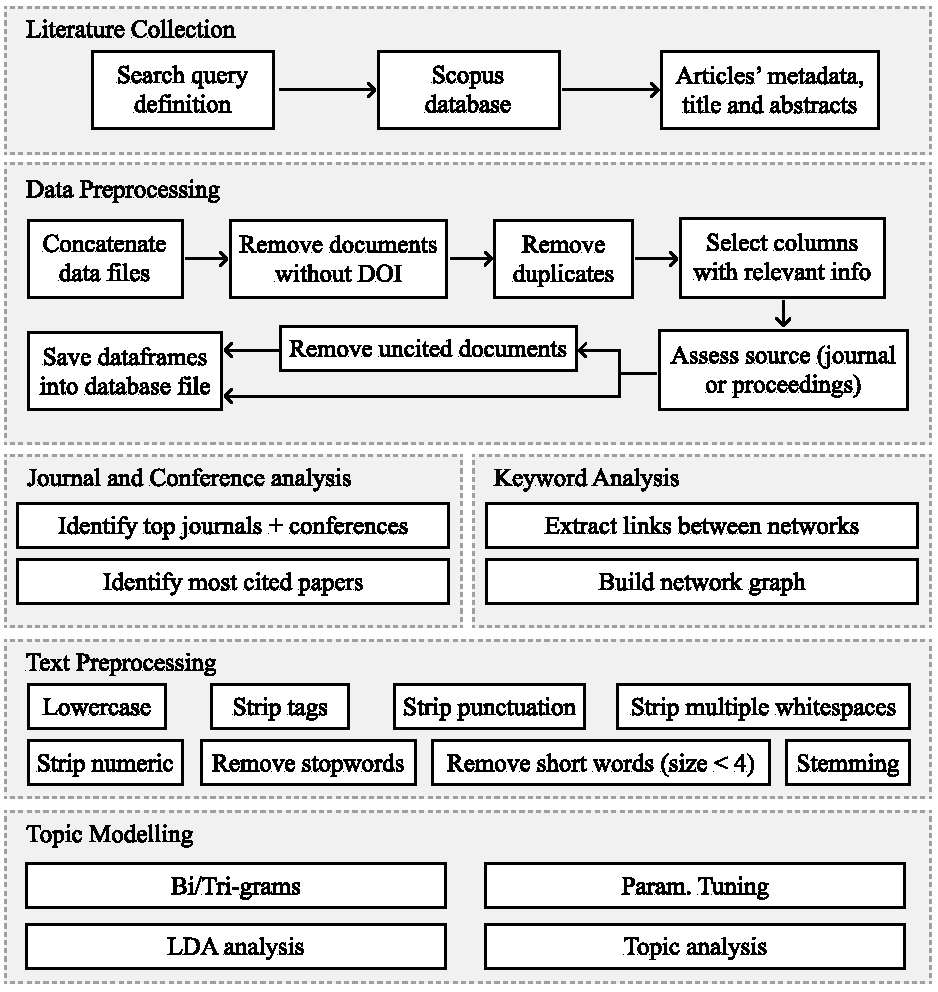
\includegraphics[width=.85\linewidth]{slr_diagram}
    \caption{Diagram of the proposed literature analysis approach.
    }~\label{fig:slr_diagram}
\end{figure}

\subsection{Literature Collection}~\label{sec:lit_collection-aug}

The focus of this literature analysis is to understand the different
algorithms, domains and/or tasks that employ data augmentation techniques.
Therefore, we search for documents containing the keyword ``data
augmentation'' in the search query. The results were then limited to
conference papers and journal articles written in English that were published
in the past 15 years.  Due to the large amount of results found, using solely
the \href{https://www.scopus.com/}{Scopus} database was found to be
sufficient. One of the goals during the search query design was to come up
with a simple and unbiased query. The resulting query is shown below:

\begin{verbatim}
    KEY ("data augmentation") AND (LIMIT-TO (LANGUAGE, "English"))  
    AND (LIMIT-TO (DOCTYPE, "cp") OR LIMIT-TO (DOCTYPE, "ar"))  
    AND (LIMIT-TO (PUBYEAR, 2021) OR LIMIT-TO (PUBYEAR, 2020)  
     OR  LIMIT-TO (PUBYEAR, 2019) OR LIMIT-TO (PUBYEAR, 2018)  
     OR  LIMIT-TO (PUBYEAR, 2017) OR LIMIT-TO (PUBYEAR, 2016)  
     OR  LIMIT-TO (PUBYEAR, 2015) OR LIMIT-TO (PUBYEAR, 2014)  
     OR  LIMIT-TO (PUBYEAR, 2013) OR LIMIT-TO (PUBYEAR, 2012)  
     OR  LIMIT-TO (PUBYEAR, 2011) OR LIMIT-TO (PUBYEAR, 2010)  
     OR  LIMIT-TO (PUBYEAR, 2009) OR LIMIT-TO (PUBYEAR, 2008)  
     OR  LIMIT-TO (PUBYEAR, 2007) OR LIMIT-TO (PUBYEAR, 2006))  
\end{verbatim}
\bigskip

The search query resulted in 4281 documents. The resulting data
selection/filtering pipeline is shown in
Figure~\ref{fig:data_filtering_pipeline}. Due to the limitations in the Scopus
data export (maximum 2000 documents per export), the data was split in four
different time periods and exported separately: 2006 until 2018, 2019, 2020
and 2021, which produced four CSV files.

\subsection{Data Preprocessing}~\label{sec:data_preprocessing-aug}

The data preprocessing stage and amount of documents dropped is represented in
Figure~\ref{fig:data_filtering_pipeline}. The data was first concatenated into
a single data frame. During this process, we found that one of the exported
references had a corrupted line, which caused the loss of one additional
document.  Since the DOI can be used as a unique identifier for intellectual
property~\cite{Paskin1999}, references without a DOI were disregarded from
further analysis, while the ones with the same identifiers are removed
(\textit{i.e.}, only one of the repeating entries is kept).

This dataset was kept to perform the analysis described in
Subsection~\ref{sec:journal_and_conference_analysis-aug}. However, further
preprocessing was done for the remaining parts of the literature analysis.
References without any citations were excluded for the keyword network and
topic modelling analyses. Finally, only the documents containing keywords in
Scopus' database were used to prepare the network analysis.

\begin{figure}
	\centering
    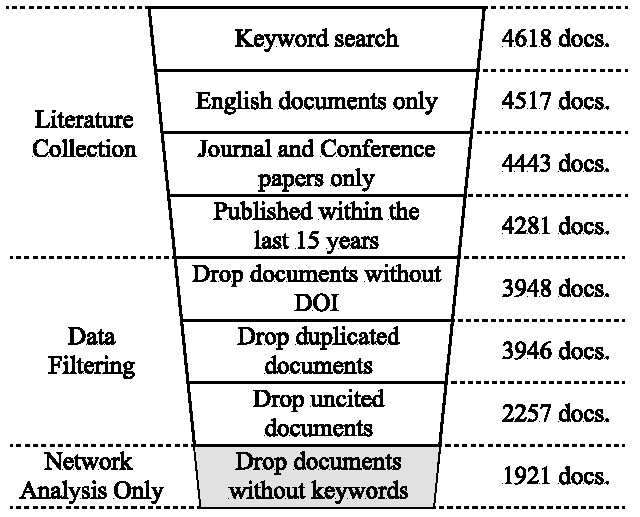
\includegraphics[width=.6\linewidth]{data_filtering_pipeline}
    \caption{Data filtering pipeline.
    }~\label{fig:data_filtering_pipeline}
\end{figure}

\subsection{Journal and Conference
analysis}~\label{sec:journal_and_conference_analysis-aug}

The exploratory analysis developed on the preprocessed dataset was targeted
towards the identification of the most significant works, journals and
conferences. We used the citation count as a proxy to understand the impact of
a specific manuscript within the research community.

The identification of the most significant conferences and journals is done by
sorting each type of publication according to the number of citations per
document. Conferences and journals with less than 10 papers published in the
area are not considered in this analysis. 

\subsection{Keyword Analysis}~\label{sec:keyword_analysis-aug}

The analysis of keywords is expected to uncover general trends in data
augmentation research and its applications. The keyword ``data augmentation''
was removed since it would link with all other keywords. Keywords are
connected based on their co-occurrence in each research paper to form the
edges of the network.  It consists of an undirected graph whose weights are
based on the total citation count for the papers containing a given keyword
pair and is calculated as $\textrm{weight} = \log(\textrm{citations}) + 1$ to
avoid a potential bias caused by highly cited research articles. The size of
the nodes were determined with a logarithmic transformation of each
node's page rank.

Keyword combinations showing up in only one document are removed from further
analysis. The keyword network is then analysed using Python and the
communities were found using the greedy modularity maximization algorithm
proposed in~\cite{Clauset2004}. The results of the analysis and community
detection were ported to Gephi to produce the final visualizations.

\subsection{Topic Modelling}~\label{sec:topic_modelling-aug}

The extraction of topics was done using the publication's abstracts. The words
were tokenized and all tags, special characters, punctuation, multiple white
spaces, numeric values, stop words and words with size smaller than 4 were
removed. Finally, we enriched the corpus by constructing bi-grams and
tri-grams.

We used a Latent Dirichlet Allocation (LDA) model~\cite{Pritchard2000} to
infer the topics present in our research domain. The tuning of the parameters
was done through experimentation and qualitative interpretation of the results
achieved. Additionally, the coherence score curve was also used as a reference for
parameter tuning and the choice of parameters, which are described in
Table~\ref{tab:hyperparameters}. 

\begin{table}[ht]
    \begin{center}
    \begin{tabular*}{.5\textwidth}{@{\extracolsep{\fill}}lllllll@{\extracolsep{\fill}}}
        \toprule
        Model   &   Hyperparameter  &   Value \\
        \midrule
        LDA     &   Num Topics      &   8     \\
                &   Chunk Size      &   2000  \\
                &   Passes          &   20    \\
                &   Alpha           &   0.1   \\
                &   ETA             &   auto  \\
        \bottomrule
    \end{tabular*}
    \caption{Hyperparameters used.}~\label{tab:hyperparameters}
    \end{center}
\end{table}

\subsection{Software Implementation}~\label{sec:software_implementation-aug}

The analysis and modelling was developed using the Python programming
language, along with the
\href{https://scikit-learn.org/stable/}{Scikit-Learn}~\cite{Pedregosa2011},
\href{https://radimrehurek.com/gensim/}{Gensim}~\cite{Rehurek2010}, and
\href{https://networkx.org/}{Networkx}~\cite{Hagberg2008} libraries. The final
network analysis and visualization was done with
\href{https://gephi.org/}{Gephi}~\cite{Bastian2009}. All functions,
algorithms, analyses and results are provided in the
\href{https://github.com/joaopfonseca/publications}{GitHub repository of the
project}.

\section{Results \& Discussion}~\label{sec:results_discussion-aug}

The popularity of research in data generation has grown significantly in the
past 5 years, as shown in Figure~\ref{fig:area_chart_cited_documents}. Despite
the significant amount of uncited publications, out of the ones published in
2020, 39\% have already been used in other works. Although most of the
research developed before 2016 was used in other works, the amount of cited
research increased significantly after that period.

\begin{figure}
	\centering
    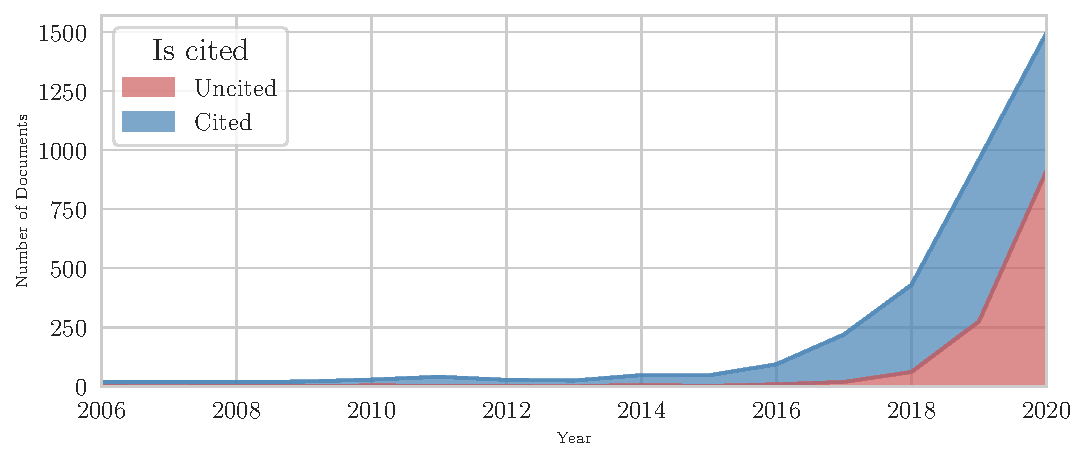
\includegraphics[width=\linewidth]{area_chart_cited_documents}
    \caption{Annual number of publications containing the keyword ``data
        augmentation''.
    }~\label{fig:area_chart_cited_documents}
\end{figure}

\subsection{Journal and Conference Analysis}

The initial exploration of the bibliometric data allows us to assess which
journals focused in data augmentation more intensely over the past years, as
shown in Table~\ref{tab:top_journals}. Most of the top journals belong to
technical fields, predominantly from Statistics, Remote Sensing, Medical
Imaging and other domains of applications such as agriculture. In addition,
all these journals have a high impact in their respective fields (based on
\href{https://www.scimagojr.com/}{Scimago Journal \& Country Rankings}).   

\begin{table}[ht]
    \begin{center}
    \begin{tabular*}{\textwidth}{@{\extracolsep{\fill}}lllllll@{\extracolsep{\fill}}}
        \toprule
        Source title & Publications & Citations & Average \\
        \midrule
        Journal of the American Statistical Association & 11 & 538 & 48.91 \\
        IEEE Geoscience and Remote Sensing Letters & 19 & 552 & 29.05 \\
        Neurocomputing & 35 & 808 & 23.09 \\
        Expert Systems with Applications & 14 & 283 & 20.21 \\
        Medical Image Analysis & 15 & 288 & 19.20 \\
        Neural Networks & 10 & 190 & 19.00 \\
        Journal of Computational and Graphical Statistics & 23 & 433 & 18.83 \\
        Computers and Electronics in Agriculture & 15 & 219 & 14.60 \\
        Biometrics & 13 & 163 & 12.54 \\
        IEEE Transactions on Medical Imaging & 10 & 123 & 12.30 \\
        \bottomrule
    \end{tabular*}
    \caption[Top journals focusing on data augmentation techniques]{%
        Top journals focusing on data augmentation techniques, sorted by
        citations per document.
    }~\label{tab:top_journals}
    \end{center}
\end{table}

Citation-wise, the publications coming from conference proceedings tend to
have a comparable impact in the research community, as shown in
Table~\ref{tab:top_conferences}. The most relevant conferences are positioned
in the computer science and information management fields. Research developed
in other areas of application, such as computer vision, speech recognition,
acoustic modelling, natural language processing and signal processing have
more activity in the form of conference proceedings publications. Conversely,
the domains most frequent in journal publications are not as active on
conference proceedings publications.

\begin{table}[ht]
    \begin{center}
    \begin{tabular*}{\textwidth}{@{\extracolsep{\fill}}lllllll@{\extracolsep{\fill}}}
        \toprule
        Source title & \# Pubs. & Cited & Avg \\
        \midrule
        Proceedings of the IEEE Computer Society Conference & 49 & 2111 & 43.08 \\
        \vspace{.2cm}on Computer Vision and Pattern Recognition &&& \\
        Lecture Notes in Computer Science (including subseries & 372 & 14946 & 40.18 \\
        Lecture Notes in Artificial Intelligence and Lecture Notes &&& \\ 
        \vspace{.2cm}in Bioinformatics) &&& \\

        \vspace{.2cm}Procedia Computer Science & 13 & 288 & 22.15 \\

        International Conference on Information and Knowledge & 10 & 180 & 18.00 \\
        \vspace{.2cm}Management, Proceedings &&& \\

        IEEE Computer Society Conference on Computer Vision & 23 & 314 & 13.65 \\
        \vspace{.2cm}and Pattern Recognition Workshops &&& \\

        ICASSP, IEEE International Conference on Acoustics, & 95 & 1153 & 12.14 \\
        \vspace{.2cm}Speech and Signal Processing - Proceedings &&& \\

        Proceedings - International Symposium on Biomedical & 30 & 346 & 11.53 \\
        \vspace{.2cm}Imaging &&& \\

        Proceedings of the International Conference on Document & 17 & 158 & 9.29 \\
        \vspace{.2cm}Analysis and Recognition, ICDAR &&& \\

        Proceedings of International Conference on Frontiers & 13 & 113 & 8.69 \\
        \vspace{.2cm}in Handwriting Recognition, ICFHR &&& \\

        2019 IEEE Automatic Speech Recognition and & 12 & 84 & 7.00 \\
        Understanding Workshop, ASRU 2019 - Proceedings &&& \\
        \bottomrule
    \end{tabular*}
    \caption[Top conferences focusing on data augmentation techniques]{%
        Top conferences focusing on data augmentation techniques, sorted by
        citations per document.
    }~\label{tab:top_conferences}
    \end{center}
\end{table}

The papers with the highest citation count are listed in
Table~\ref{tab:top_papers}. We found that much of the research focused on
improving deep learning classification, segmentation or object detection
without a focus on a particular domain of application. Other papers centered
in the application of data augmentation methods for biomedical image
classification and segmentation, sound and speech recognition and remote
sensing.

\begin{table}[ht]
    \begin{center}
    \begin{tabular*}{\textwidth}{@{\extracolsep{\fill}}lllllll@{\extracolsep{\fill}}}
        \toprule
        Authors & Title & Year & Cited \\
        \midrule
        Ronneberger O., Fischer P., & U-net: Convolutional networks & 2015 & 13597 \\
        \vspace{.2cm}Brox T. & for biomedical image segmentation && \\

        Chatfield K., Simonyan K., & Return of the devil in the details: & 2014 & 1885 \\
        \vspace{.2cm}Vedaldi A., Zisserman A. & Delving deep into convolutional nets && \\

        Snyder D., Garcia-Romero D., & X-Vectors: Robust DNN Embeddings & 2018 & 636 \\
        \vspace{.2cm}Sell G., Povey D., Khudanpur S. & for Speaker Recognition && \\

        Shorten C., Khoshgoftaar T.M. & A survey on Image Data & 2019 & 590 \\
        \vspace{.2cm}                 & Augmentation for Deep Learning && \\

        Salamon J., Bello J.P. & Deep Convolutional Neural Networks & 2017 & 505 \\
                               & and Data Augmentation for \\
        \vspace{.2cm}          & Environmental Sound Classification \\

        Eitel A., Springenberg J.T., & Multimodal deep learning for robust & 2015 & 352 \\
        Spinello L., Riedmiller M., & RGB-D object recognition && \\
        \vspace{.2cm}Burgard W. &&& \\

        Ding J., Chen B., Liu H., & Convolutional Neural Network with & 2016 & 319 \\
        Huang M.                  & Data Augmentation for SAR Target && \\
        \vspace{.2cm}             & Recognition \\

        Wong S.C., Gatt A., & Understanding Data Augmentation & 2016 & 302 \\
        \vspace{.2cm}Stamatescu V., McDonnell M.D. & for Classification: When to Warp? && \\

        Frid-Adar M., Diamant I., & GAN-based synthetic medical image & 2018 & 296 \\
        Klang E., Amitai M., & augmentation for increased CNN && \\
        Goldberger J., Greenspan H. & performance in liver lesion && \\
        \vspace{.2cm}               & classification \\

        Bilen H., Vedaldi A. & Weakly Supervised Deep Detection & 2016 & 287 \\
        \vspace{.2cm}        & Networks \\

        \bottomrule
    \end{tabular*}
    \caption[Top papers using data augmentation techniques.]{%
        Top papers using data augmentation techniques, sorted by citation
        count.
    }~\label{tab:top_papers}
    \end{center}
\end{table}

\subsection{Keyword Analysis}

The keyword network shown in Figure~\ref{fig:keyword_network} revealed 8 main
communities of keywords, and 13 other small communities. The different
communities are distinguished by the type of algorithms used and/or the domain
of application. The main distinctive factor for the larger communities are the
types of generative models used, while the smaller communities are
distinguished according to the domain of application. The most significant
findings we found from this analysis are:

\begin{enumerate}
    \item The community marked with pink-colored nodes is characterized by the
        usage of neural network-based data augmentation methods in
        convolutional neural networks. The keyword ``deep learning'' is
        positioned as a central node (although not labelled in the figure to
        maintain readability). Other relevant keywords are related to
        machine/deep learning frameworks, deep learning classifiers and data
        augmentation algorithms, such as ``tensorflow'', ``keras'',
        ``convolutional neural network'' and ``generative adversarial
        networks''. Domain specific keywords are also present:
        \begin{itemize}
            \item Medical keywords located in this community cover a variety
                of applications. Relevant sub communities are [``hand
                writing'', ``parkinson's disease (pd)'', ``transfer
                learning''], [``breast cancer'', ``computer-aided
                detection''], [``melanoma'', ``skin cancer'', ``image
                processing'', ``googlenet''], [``chest x-ray'',
                ``computer-aided diagnosis'', ``tuberculosis'',
                ``segmentation''] and [``brain'', ``mri'', ``multiple
                sclerosis'']. 
            \item Remote sensing keywords are typically related to
                classification and object detection tasks. Relevant sub
                communities are [``object detection'', ``aerial image'',
                ``drone'', ``generative adversarial network'', ``semantic
                segmentation''], [``attributed scattering center (asc)'',
                ``synthetic aperture radar (sar)'', ``convolutional neural
                network (cnn)''], [``remote sensing'', ``road extraction'',
                ``transfer learning'', ``generative adversarial network''].
                Keywords such as ``hyperspectral imaging'' and ``weather
                classification'' are also scattered around the community.
            \item Facial recognition research is also represented in few sub
                communities: [``micro expression recognition'', ``small
                training data'', ``convolutional neural network (cnn)'', ``local
                binary pattern-three orthogonal planes (lbp-top)''] and
                [``training data augmentation'', ``sequence-to-sequence speech
                synthesis'', ``sequence-to-sequence speech recognition''].
            \item Fault detection studies also used data augmentation to deal
                with imbalanced datasets: [``fault diagnosis'', ``imbalanced
                data'', ``gan'']
            \item Data augmentation was also associated to regularization
                methods and feature extraction tasks, based on the presence of
                the sub communities [``overfitting'', ``dropout'' and ``cnn'']
                and [``feature extraction'', ``cnn'', ``svm''].
        \end{itemize}
    \item The community marked with blue-colored nodes is characterized by the
        usage of Markov Chain-based algorithms. The keywords ``markov chain'',
        ``data augmentation algorithm'' and ``monte carlo'' appear as central
        nodes. No application-specific sub-community was found.
    \item The community marked with green-colored nodes is characterized by
        the usage of Markov Chain and Bayesian-based algorithms. The keywords
        ``bayesian inference'', ``markov chain monte carlo'', ``mcmc'',
        ``bayesian analysis'', ``missing data'' and ``em algorithm''
        (expectation maximization algorithm). Application-specific keywords
        may be found sparsely distributed across the community, all of them
        related to biological applications. Specifically, the sub community
        [``ecological health'', ``stressor-response'', ``biological
        monitoring'', ``bayesian methods''] and the keyword ``camera
        trapping'' were found in this community. 
    \item The community marked with orange-colored nodes is characterized by
        keywords specific to big data and data warehousing applications. The
        network is composed of the keywords ``big data'', ``data lake'',
        ``olap'', ``map reduce'', ``cmm'', ``data warehouse'',
        ``augmentation'' and ``dm''.
    \item The remaining communities consist mostly of data augmentation
        methods applied to specific domains. Specifically, the usage of
        temporal-dynamic neural network architectures with ``eeg
        (electroencephalogram)'', music information retrieval applications
        (e.g., ``chord recognition''), speech/ speaker recognition and
        embedding, time series forecasting of diabetes and natural language
        processing and text classification.
\end{enumerate}

\begin{figure}[ht]
	\centering
    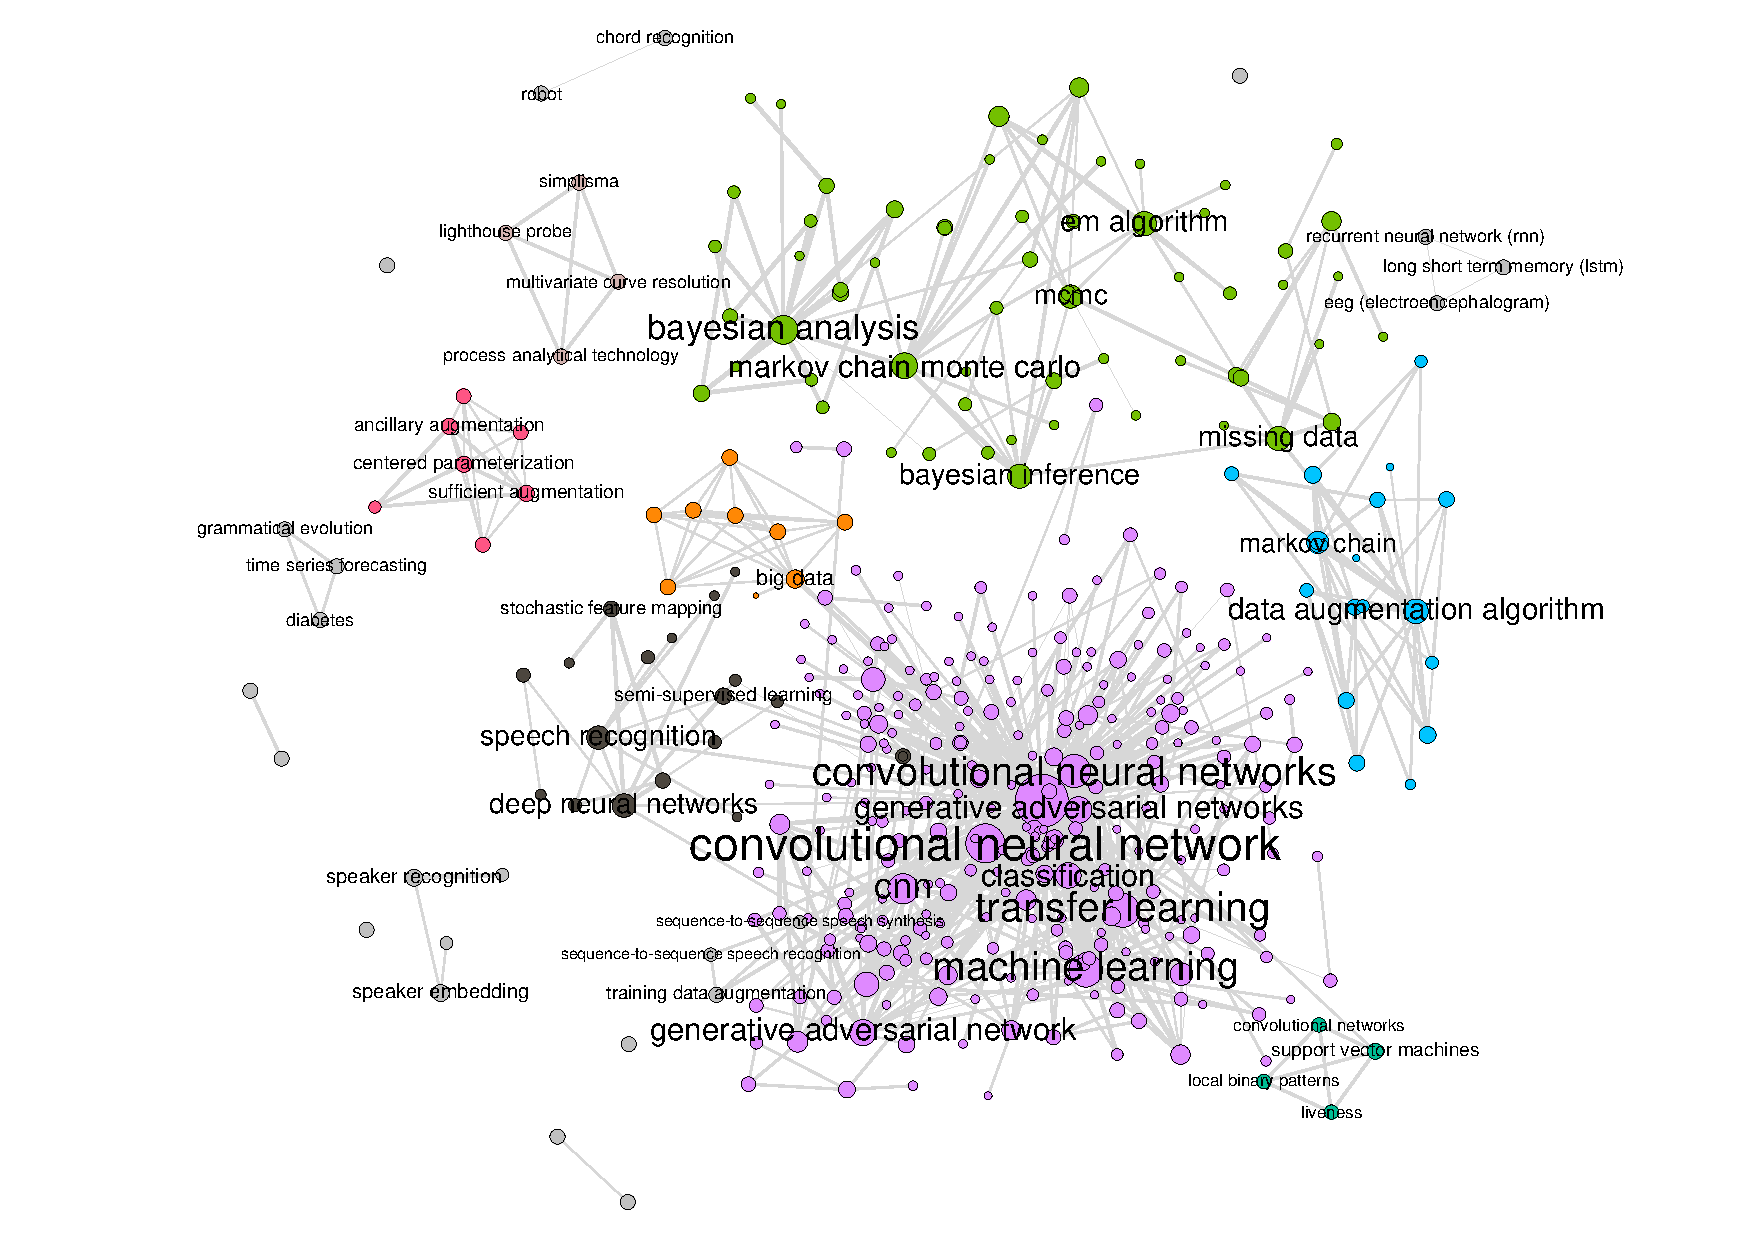
\includegraphics[width=\linewidth]{keyword_network}
    \caption{Keyword network.
    }~\label{fig:keyword_network}
\end{figure}

\subsection{Topic Analysis}

The LDA topic extraction resulted in 8 different topics, whose distribution of
topics is shown in Figure~\ref{fig:lda_topics_sankey}. The main topics within
which most articles were included is topic 5, which is defined by the main
theoretical keywords related to image data augmentation. Rather, the secondary
topic is more useful for this analysis. It is found based on the topic
likelihood of each document, excluding the dominant topic. Documents belonging
to the same group across primary, secondary and/or tertiary topics had a
likelihood of zero of belonging to any other topic.

\begin{figure}[ht]
	\centering
    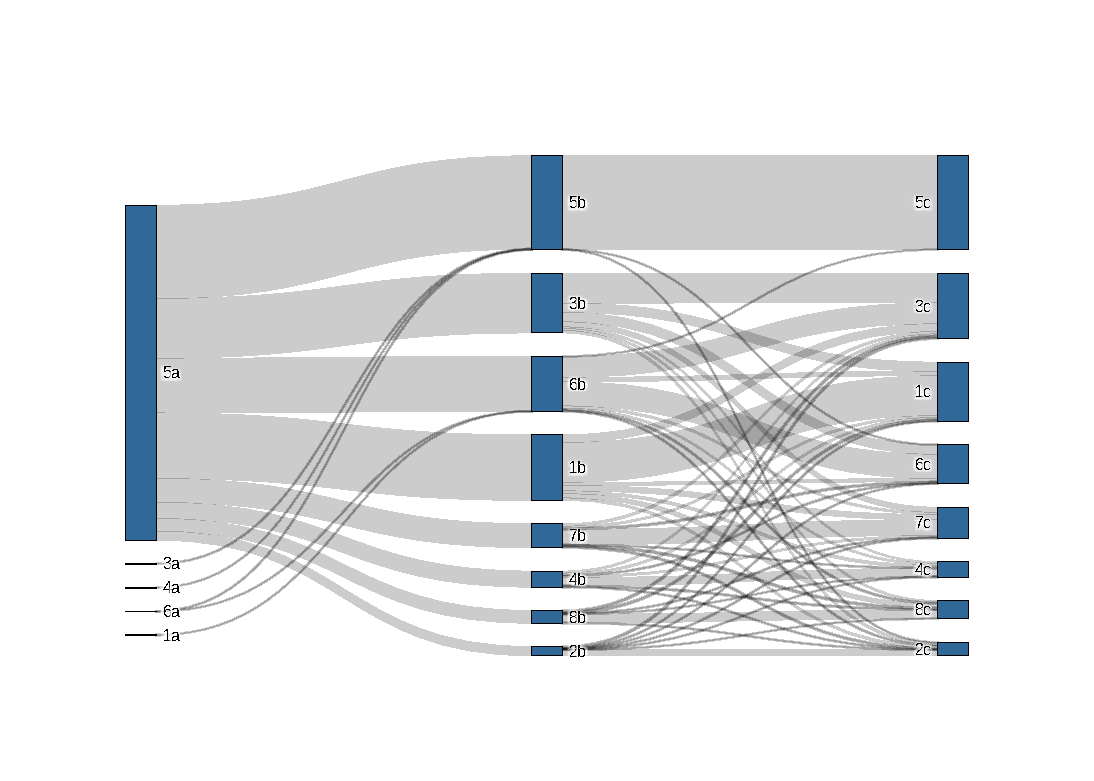
\includegraphics[width=\linewidth]{lda_topics_sankey}
    \caption[Distribution of documents over the different topics
    found.]{%
        Distribution of documents over the different topics found. The
        left column represent the primary topics, the middle column represents
        the secondary topics and the right columns represents the tertiary
        topics.
    }~\label{fig:lda_topics_sankey}
\end{figure}

The topics found in the bibliometric data are shown in
Table~\ref{tab:topic_analysis}. A few topics seem to overlap each other,
although they are generally distinguishable. The primary domains of
application of data augmentation methods differ for each different topic
identified:

\begin{enumerate}
    \item Documents in Topic 1 frequently use the word ``yolov'', which refers
        to the YOLOvX family of deep learning object detection
        models~\cite{Redmon2015}, where X refers to the version of the model
        used (the most recent version is 5). Another relevant keyword is
        ``style\_transfer'', which refers to a specific technique of data
        augmentation. 

        This topic has two primary domains of application. The keywords
        ``pest'' and ``coffe'' refer to data augmentation on agriculture
        research. The keywords ``biomed'', ``histolog'' and ``nodul'' refer to
        biomedical applications such as pulmonary nodule detection and
        histology image classification. Within these topics, a few
        domain-specific data augmentation algorithms were proposed. For
        example, in~\cite{Cicalese2020} the authors propose a style-transfer
        data augmentation method for histology image classification.  

    \item Documents in Topic 2 are primarily associated to the study of
        applications that include image data augmentation. The dominant
        keyword, ``hyperspectr\_imag'', refers to the application of data
        augmentation on hyperspectral images, commonly used in remote sensing
        and medicine. Other classification tasks include license plate
        detection (``licens\_plate''), inpainting (``inpaint''), background
        subtraction (``illumin\_chang'') and cloud shadow
        detection/segmentation (``shadow'').
    
    \item Documents in topic 3 refer to the application of data augmentation
        to deal with censored data (a condition in which the value of an
        observation is only partially known) and/or supervised tasks on data
        structured as graphs. Other domains of application involve chest
        x-rays classification (``cxr''), epidemiology (``risk\_factor'') and
        few audio/music information retrieval (``sourc\_separ'') articles.

    \item Documents in topic 4 refer to the application of data augmentation
        methods on object detection tasks. Specifically fire and smoke,
        pedestrians and crowd counting. Other applications within this topic
        are focused on speech recognition and angiography
        segmentation/classification.

    \item Documents in topic 5 are focused on image segmentation
        and classification methods where data augmentation algorithms are
        involved. It includes common keywords present in a large set of
        articles. These articles are mainly focused on the development of
        different convolutional neural network architectures (``cnn'') and
        neural network-based data augmentation methods.

    \item Documents in topic 6 are focused on Bayesian-based algorithms and
        Markov Chain algorithms. This topic includes data augmentation on
        regression tasks and misclassification detection.

    \item Documents in topic 7 covers the application of data augmentation
        into various domains. Specifically, music information retrieval
        (``music''), fish/marine organisms recognition, gender bias, speech
        recognition, random erasing 

    \item Documents in topic 8 contains remote sensing and biomedicine as the
        primary research domains. The keywords ``drone'' and ``aircraft''
        refer to the sources of data collected for remote sensing work,
        whereas ``pneumonia'' and ``chest\_rai\_imag'' refers to biomedicine
        research topics/image data.
\end{enumerate}


\begin{table}
    \begin{center}
    \begin{tabular*}{\textwidth}{@{\extracolsep{\fill}}lllllll@{\extracolsep{\fill}}}
        \toprule
        Topic & Representative Paper & Papers & Words\\
        \midrule
        1 & GAN-based synthetic medical image & 440 & yolov, pest, style\_transfer, \\
          & augmentation for increased CNN && coffe, thermal, biomed, \\
          & performance in liver lesion && scene\_text, histolog, nodul, \\
        \vspace{.2cm}& classification && visibl \\
        
        2 & CVAE-GAN: Fine-Grained Image & 61 & hyperspectr\_imag, licens\_plate, \\
          & Generation through Asymmetric && command, inpaint, \\
          & Training && illumin\_chang, upper, restor, \\
        \vspace{.2cm}  &&& ann, foreign, shadow \\
        
        3 & A survey on Image Data & 401 & censor, markov\_chain, node, \\ 
          & Augmentation for Deep Learning && team, tree, cxr, risk\_factor, \\
        \vspace{.2cm}  &&&mass, largest, sourc\_separ\\
        
        4 & Return of the devil in the details: & 108 & smoke, pedestrian, transcrib, \\
          & Delving deep into convolutional nets && crowd, children\_speech, intent, \\
          &&&adult, auxiliari\_variabl, speech, \\
        \vspace{.2cm}  &&&angiographi \\
        
        5 & U-net: Convolutional networks for & 632 & imag, detect, gener, dataset, \\
          & biomedical image segmentation && classif, sampl, network, cnn, \\
        \vspace{.2cm}  &&&featur, augment\\
        
        6 & Deep Convolutional Neural Networks & 370 & tea, multivari, \\
          & and Data Augmentation for && markov\_chain\_mont\_carlo, \\
          & Environmental Sound Classification && bayesian, regress, misclassif, \\
        \vspace{.2cm}  &&& procedur, famili, illustr, mcmc \\
        
        7 & Weakly Supervised Deep Detection & 160 & music, fish, marin, gender, \\
          & Networks && vocal, random\_eras, low\_qualiti, \\
        \vspace{.2cm}  &&& crowd, prune, bengali \\
        
        8 & An Efficient Deep Learning Approach & 85 & drone, gait, aircraft, \\      
          & to Pneumonia Classification in && gestur\_recognit, pneumonia, \\
          & Healthcare && chest\_rai\_imag, covid, walk, \\
          &&& onset, hidden\_layer \\
        \bottomrule
    \end{tabular*}
    \caption{%
        Description of the main topics found in the literature.
    }~\label{tab:topic_analysis}
    \end{center}
\end{table}

The per-year popularity of the different topics is shown in
Figure~\ref{fig:topics_per_year}. Since 2015, topic 5 gained more research
momentum, whereas topic 6 lost much of its relative popularity within the
field. In the past 5 years topics 8 and 3 have become steady research streams
while topic 1 saw a significant growth in popularity. 

\begin{figure}
	\centering
    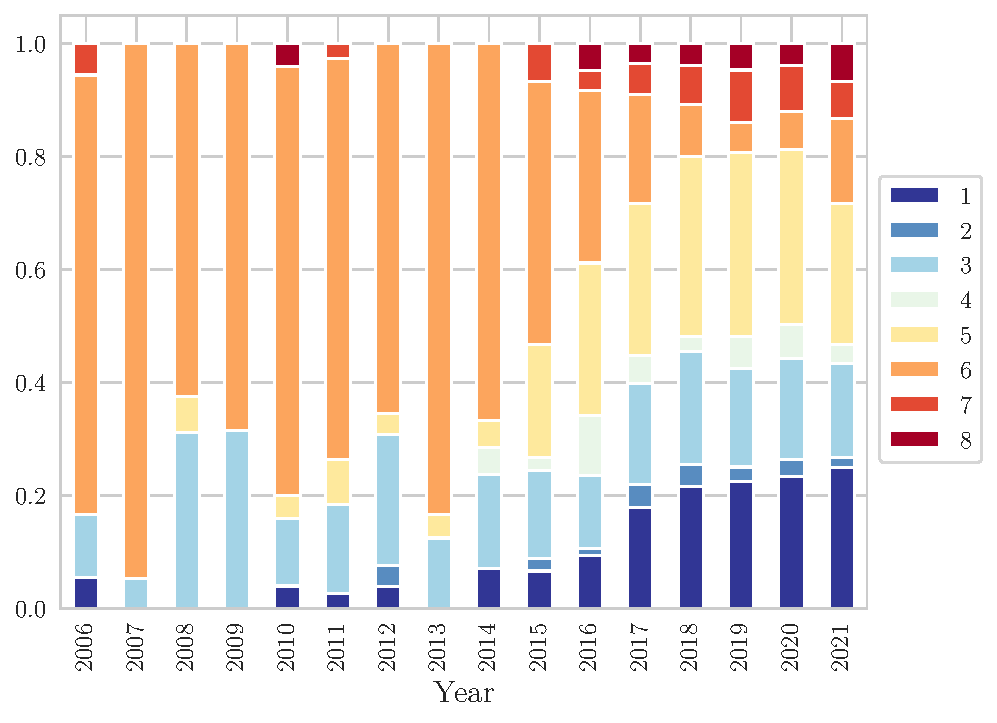
\includegraphics[width=.8\linewidth]{topics_per_year}
    \caption{Topic frequency per year.
    }~\label{fig:topics_per_year}
\end{figure}

\subsection{Research Gap Discussion}

Data augmentation mechanisms are often used as regularization methods for
deep learning classifiers. The study of data augmentation mechanisms in
ensembles of simple classifiers have achieved state-of-the-art performance not
only 10 years ago~\cite{Meier2011, Ciresan2011}, but also when compared to
modern deep learning architectures~\cite{Tolstikhin2021, Touvron2021,
Liu2021}. However, the implementation of different data augmentation methods
shows a promising path to improve the performance of simple classifiers
(and/or recent ensemble architectures) and requires further research.

A research application that was not frequently found in the literature was
small dataset augmentation. This is particularly useful for any complex
problem when the amount of labeled data available to use as training data is
scarce, which limits the usage of classification algorithms and especially
deep learning algorithms. In this context, techniques such as Active Learning
can be used to annotate a small amount of data, while maximizing the
classification performance~\cite{Su2020}. However, classifiers may not be
capable of generalizing with small training datasets and the ability to
reproduce and augment the labelled data available can further reduce
annotation cost and allow the usage of data intensive classifiers.

Another limitation found in the literature relates to the problem of
initialization on network-based data augmentation methods. The same data
augmentation algorithm trained with different initialization settings
(different random seed or training subset) may lead to different model
parameters and quality of the trained classifier.

The rapid development of data augmentation algorithms raises additional open
questions on how the data used and store for model training. Specifically, the
lower data storage and processing power available to the general public
(\textit{i.e.}, organizations and individuals) is a limitation for producing
state-of-the-art classifiers. Another problem arises from data privacy
concerns, since the usage of user data to train machine learning models
typically involve the storage of such information. However, if data
augmentation algorithms were continuously updated and capable of producing
reliable data on an as-needed basis, not only would storage requirements
decrease, but it would also become possible to work with fully artificial
data, without the need to store as much data. This would also facilitate the
sharing of datasets (in the form of an algorithm) without compromising
sensitive data.

\section{Conclusion}~\label{sec:conclusion-aug}

Depending on the domain of application, data augmentation research differs in
the format of publication. On the one hand, domains like Statistics, Remote
Sensing and Medical Imaging seem more active on journal publications,
typically in journals with high impact factor. On the other hand, research
developed in the domains of computer vision, speech recognition, acoustic
modelling, natural language processing and signal processing seem to attribute
higher importance to conference papers. Many of the influential papers we found
were focused on deep learning methods for classification, segmentation, sound
and speech recognition and remote sensing.

We analysed the different communities of keywords formed using document
keywords, as well as topic analysis using a LDA analysis over the document's
abstracts. We found various distinctive areas of research, both regarding the
data augmentation methods used and the domain of application. We found that in
recent years research on augmentation methods using Bayesian-based algorithms,
as well as Markov Chain algorithms reduced its popularity, whereas data
augmentation methods based on neural networks and deep learning classifiers
have increased its popularity.

Data augmentation is most commonly applied/studied in the realm of computer
vision for tasks like image classification, segmentation, object detection,
inpainting and background subtraction tasks, even though it may be applied to
many other data structures. It is frequently used in studies within the
domains of biomedicine, agriculture, speech recognition, acoustic modelling,
remote sensing and computational creativity. It is also used alongside other
data preprocessing techniques, such as feature extraction and dimensionality
reduction.

Although data augmentation is a vibrant area of research, there are still
significant gaps to be addressed. Data augmentation methods are increasingly
used as regularization methods for deep learning. Although, recent research
shows that the same can be done for simpler classifier configurations in order
to achieve a classification performance comparable to that of state-of-the-art
deep learning, which require further confirmation, as well as the development
of less computational intensive data augmentation methods. Other less popular
topics, such as small data augmentation, appear to have a relevant practical
importance and require further research. In addition, other limitations of
data augmentation algorithms should be addressed. One problem commonly found
in the literature is the impact the weights initialization and training set
used have in the quality of the trained algorithm. In the future, using data
augmentation methods as a source of artificial datasets can address a variety
of concerns, such as data privacy, sharing and storage. Finally, exploring
data augmentation algorithms to complement or replace techniques such as
Active Learning may reduce the cost of data collection, although it is yet to
be explored.

\thesischapter{%
    Improving Imbalanced Land Cover Classification with K-means SMOTE\@:
    Detecting and Oversampling Distinctive Minority Spectral Signatures
}{%
    Published as Joao Fonseca, Georgios Douzas, Fernando Bacao, in Information
    Journal, 2021
}~\label{chp:kmeans-smote}


\graphicspath{{figures/kmeans-smote-lulc/}}

\begin{adjustwidth}{30pt}{30pt}

    Land cover maps are a critical tool to support informed policy
    development, planning, and resource management decisions. With significant
    upsides, the automatic production of Land Use/Land Cover maps has been a
    topic of interest for the remote sensing community for several years, but
    it is still fraught with technical challenges. One such challenge is the
    imbalanced nature of most remotely sensed data. The asymmetric class
    distribution impacts negatively the performance of classifiers and adds a
    new source of error to the production of these maps. In this paper, we
    address the imbalanced learning problem, by using K-means and the
    Synthetic Minority Oversampling TEchnique (SMOTE) as an improved
    oversampling algorithm.  K-Means SMOTE improves the quality of newly
    created artificial data by addressing both the between-class imbalance, as
    traditional oversamplers do, but also the within-class imbalance, avoiding
    the generation of noisy data while effectively overcoming data imbalance.
    The performance of K-means SMOTE is compared to three popular oversampling
    methods (Random Oversampling, SMOTE and Borderline-SMOTE) using seven
    remote sensing benchmark datasets, three classifiers (Logistic Regression,
    K-Nearest Neighbors and Random Forest Classifier) and three evaluation
    metrics using a 5-fold cross-validation approach with 3 different
    initialization seeds. The statistical analysis of the results show that
    the proposed method consistently outperforms the remaining oversamplers
    producing higher quality land cover classifications. These results suggest
    that LULC data can benefit significantly from the use of more
    sophisticated oversamplers as spectral signatures for the same class can
    vary according to geographical distribution.

\end{adjustwidth}

\vspace{.5cm}
\textbf{Keywords:} LULC Classification; Imbalanced Learning; Oversampling;
Data Augmentation; Clustering

\section{Introduction}

The increasing amount of remote sensing missions granted the access to dense
time series (TS) data at a global level and provides up-to-date, accurate land
cover information \cite{Drusch2012}. This information is often materialized
through Land Use and Land Cover (LULC) maps. While Land Cover maps
define the biophysical cover found on the surface of the earth, Land Use maps
define how it is used by humans \cite{Fritz2017}. Both Land Use and Land Cover
maps constitute an essential asset for various purposes, such as land cover
change detection, urban planning, environmental monitoring and natural hazard
assessment \cite{Khatami2016}. However, the timely production of accurate and
updated LULC maps is still a challenge within the remote sensing community
\cite{Wulder2018}. LULC maps are produced based on two main approaches:
photo-interpreted by the human eye, or automatic mapping using remotely sensed
data and classification algorithms.

While photo-interpreted LULC maps rely on human operators and can be more
reliable, they also present some significant disadvantages. The most important
disadvantage is the cost of production, in fact photo-interpretation consumes
significant resources, both in terms of money and time. Because of that, they
are not frequently updated and not suitable for operational mapping over large
areas.  Finally, there is also the issue of overlooking rare or small-area
classes, due to factors such as the minimum mapping unit being used.

Automatic mapping with classification algorithms based on machine-learning
(ML) have been extensively researched and used to speed up and reduce the
costs of the production process \cite{Khatami2016, Gavade2019,
Kaur2019}. Improvements in classification algorithms are sure to have
significant impact in the efficiency with which remote sensing imagery is
used. Several challenges have been identified in order to improve automatic
classification:

\begin{enumerate}
    \item Improve the ability to handle high-dimensional datasets, in cases
        such as Multi-spectral TS composites high-dimensionality increases the
        complexity of the problem and creates a strain on computational power
        \cite{Stromann2020}.
    \item Improve class separability, as the production of an accurate LULC map
        can be hindered by the existence of classes with similar spectral
        signatures, making these classes difficult to distinguish
        \cite{Alonso-Sarria2019}.
    \item Resilience to mislabelled LULC patches, as the use of
        photo-interpreted training data poses a threat to the quality of any
        LULC map produced with this strategy, since factors such as the minimum
        mapping unit tend to cause the overlooking of small-area LULC patches
        and generates noisy training data that may reduce the prediction
        accuracy of a classifier \cite{Pelletier2017}.
    \item Dealing with rare land cover classes, due to the varying levels of
        area coverage for each class. In this case using a purely random
        sampling strategy will amount to a dataset with a roughly proportional
        class distribution as the one on the multi/hyperspectral
        image. On the other hand, the acquisition of training
        datasets containing balanced class frequencies is often unfeasible.
        This causes an asymmetry in class distribution, where some classes are
        frequent in the training dataset, while others have little expression
        \cite{Wang2019, Feng2019}.
\end{enumerate}

The latter challenge is known, in machine learning, as the imbalanced learning
problem \cite{Chawla2004}. It is defined as a skewed distribution of instances
found in a dataset among classes in both binary and multi-class problems
\cite{Abdi2016}. This asymmetry in class distribution negatively impacts the
performance of classifiers, especially in multi-class problems.  The problem
comes from the fact that during the learning phase, classifiers are optimized
to maximize an objective function, with overall accuracy being the most common
one \cite{Maxwell2018}. This means that instances belonging to minority
classes contribute less to the optimization process, translating into a bias
towards majority classes. As an example, a trivial classifier can achieve 99\%
overall accuracy on a binary dataset where 1\% of the instances belong to the
minority class if it classifies all instances as belonging to the majority
class. This is an especially significant issue in the automatic classification
of LULC maps, as the distribution of the different land-use classes tends to
be highly imbalanced.  Therefore, improvements in the ability to deal with
imbalanced datasets will translate into important progress in the automatic
classification of LULC maps.

There are three different types of approaches to deal with the class imbalance
problem \cite{Fernandez2013,Kaur2019}:

\begin{enumerate}
    \item Cost-sensitive solutions. Introduces a cost matrix to the learning
        phase with misclassification costs attributed to each class. Minority
        classes will have a higher cost than majority classes, forcing the
        algorithm to be more flexible and adapt better to predict minority
        classes.
    \item Algorithmic level solutions. Specific classifiers are modified to
        reinforce the learning on minority classes. Consists on the creation or
        adaptation of classifiers.
    \item Resampling solutions. Rebalances the dataset's class distribution by
        removing majority class instances and/or generating artificial minority
        instances. This can be seen as an external approach, where the
        intervention occurs before the learning phase, benefitting from
        versatility and independency from the classifier used.
\end{enumerate}

Since resampling strategies represent a set of methods that are detached from
classifiers by operating at the data level, they allow the use of any off the
shelf algorithm, without the need for any type of changes or adaptions to the
algorithm. Specifically, in the case of oversampling (defined below), the user
is able to balance the dataset's class distribution by without the loss of
information, which is not the case with undersampling techniques. This is a
significant advantage especially considering that most users in remote sensing
are not expert machine learning engineers. 

Within resampling approaches there are three subgroups of approaches
\cite{Fernandez2013,Kaur2019,Luengo2020}:

\begin{enumerate}
    \item Undersampling methods, which rebalance class distribution by removing
        instances from the majority classes.
    \item Oversampling methods, which rebalance datasets by generating new
        artificial instances belonging to the minority classes.
    \item Hybrid methods, which are a combination of both oversampling and
        undersampling, resulting in the removal of instances in the majority
        classes and the generation of artificial instances in the minority
        classes.
\end{enumerate}

Resampling methods can be further distinguished between non-informed and
heuristic (i.e., informed) resampling techniques
\cite{Fernandez2013,Luengo2020,Garcia2016}. The former consist of methods that
duplicate/remove a random selection of data points to set class distributions
to user-specified levels, and are therefore a simpler approach to the problem.
The latter consists of more sophisticated approaches that aim to perform
over/undersampling based on the points' contextual information within their
data space.

The imbalanced learning problem is not new in machine learning but its
relevancy has been growing, as attested by \cite{Haixiang2017}. The problem
has also been addressed in the context of remote sensing \cite{Douzas2019rs}.
In this paper, we propose the application of a recent oversampler based
on SMOTE \cite{Chawla2002}, the K-means SMOTE 
\cite{Douzas2018} oversampler, to address the imbalanced learning
problem in a multiclass context for LULC classification using various remote
sensing datasets. Specifically, we use seven land use datasets commonly
used in research literature, that vary among agricultural and urban land use.
The K-means SMOTE algorithm couples two different
procedures in the generation of artificial data. The algorithm starts by
grouping the instances into clusters by using the K-means
algorithm; next, the generation of the artificial
data is done using the smote algorithm, taking into consideration the distribution of
majority/minority cases in each individual cluster. The idea of starting with
a clustering procedure before the data generation phase is important in remote
sensing because the spectral signature of the different classes can change
significantly based on the geographical area in which it is represented. In
other words, the spectral signature of a specific class can vary greatly
depending on the geography, meaning that often we will be facing within-class
imbalance \cite{Japkowicz2001}.

In fact, we can decompose class imbalance into two different types:
between-class imbalance and within-class imbalance \cite{Douzas2018, Jo2004}.
While the first refers to the overall asymmetry between majority and minority
classes, the second results from the fact that in different areas of the input
space there might be different levels of imbalance. Depending on the
complexity of the input space, different subclusters of minority and majority
instances may be present. In order to achieve a balance between minority and
majority instances, these subclusters should be treated separately. Assuming
that the role of a classifier is to create rules in such a way that it is able
to isolate the different relevant sub-concepts that represent both the
majority and minority classes, the classifier will create multiple disjunct
rules that describe these concepts. If the input space is simple and the
classes’ instances are grouped together in a unique cluster, the classifier
will only need to create (general) rules that comprise large portions of
instances belonging to the same class. To the contrary, if the input space is
complex and scatters through multiple small clusters, the classifier will need
to learn a more complex set of (specific) rules, which can be seen in Figure
\ref{fig:complex_input_space_example}. It is important to note that small
clusters can happen both in the minority and majority class, although they
will tend to be more frequent in the minority class due to its
underrepresentation.  

\begin{figure}[ht]
	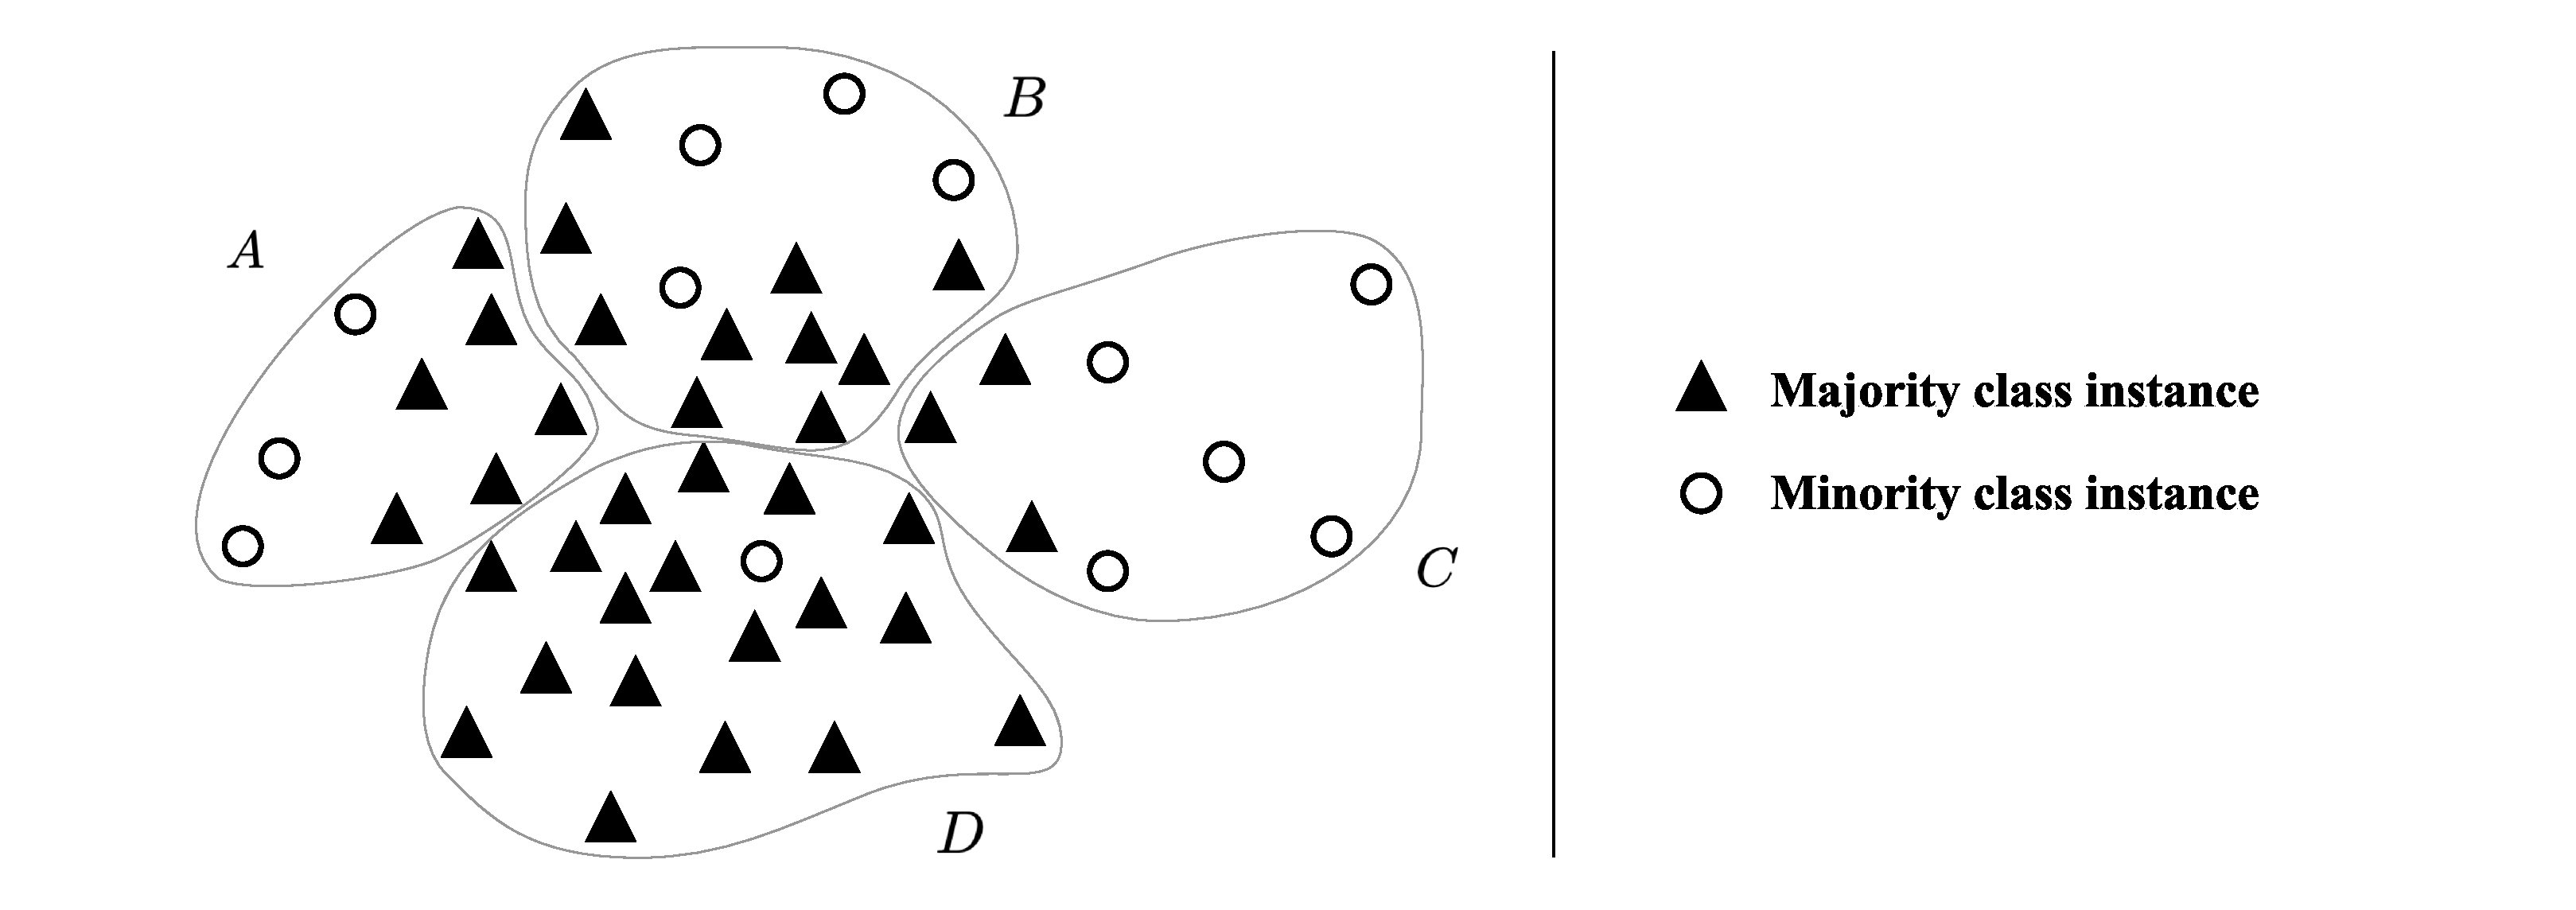
\includegraphics[width=1\linewidth]{complex_input_space_example}
    \caption[Example of a complex input space.]{%
        Example of a complex input space. In this example, a classifier
        would need to separate the minority class' samples across 4
        distinguishable clusters (A, B, C and D).
    }~\label{fig:complex_input_space_example}
\end{figure}

The efficacy of K-means SMOTE is tested using different types of classifiers.
To do so, we employ both commonly used and/or state-of-the-art oversamplers as
benchmarking methods: Random oversampling (ROS), SMOTE and Borderline-SMOTE
(B-SMOTE) \cite{Han2005}. Also as a baseline score we include classification
results without the use of any resampling method.

This paper is organized in 5 sections: section \ref{sec:sota-kmeans} provides an
overview of the state-of-art, section \ref{sec:methodology-kmeans} describes the
proposed methodology, section \ref{sec:results-kmeans} covers the results and
discussion and section \ref{sec:conclusion-kmeans} presents the conclusions taken from
this study.

This paper's main contributions are:
\begin{itemize}
    \item Propose a cluster-based multiclass oversampling method appropriate
        for LULC classification and compare its performance with the remaining
        oversamplers in a multiclass context with seven benchmark LULC
        classification datasets. Allows us to check the oversamplers'
        performance across benchmark LULC datasets.
    \item Introducing a cluster-based oversampling algorithm within the remote
        sensing domain, as well as comparing its performance with the remaining
        oversamplers in a multiclass context.
    \item Make available to the remote sensing community the implementation
        of the algorithm in a Python library and the experiment's source
        code.
\end{itemize}

\section{Imbalanced Learning Approaches}~\label{sec:sota-kmeans}

Imbalanced learning has been addressed in three different ways:
over/undersampling, cost-sensitive training and changes/adaptations in the
learning algorithms \cite{Kaur2019}. These approaches impact different
phases of the learning process, while over/undersampling can be seen as a
pre-processing step, cost-sensitive and changes in the algorithm imply a more
customized and complex intervention in the algorithms. In this
section, we focus on previous work related with resampling methods, while
providing a brief explanation of cost-sensitive and algorithmic level solutions.

All of the most common classifiers used for LULC classification tasks
\cite{Khatami2016, Gavade2019} are sensitive to class imbalance
\cite{Blagus2010}. Algorithm-based approaches typically focus on adaptations
based on ensemble classification methods \cite{Mellor2015} or common
non-ensemble based classifiers such as Support Vector Machines \cite{Shao2014}.
In \cite{Lee2016}, the reported results show that algorithm-based methods have
comparable performance to resampling methods.

Cost-sensitive solutions refer to changes in the importance attributed to each
instance through a cost matrix \cite{Huang2016,Cui2019,Dong2017}. A
relevant cost sensitive solution
\cite{Huang2016} uses  the inverse class frequency (i.e., $1/|C_i|$, where $C_i$ refers
to the frequency of class $i$) to give higher weight to
minority classes. Cui et al. \cite{Cui2019} extended this method by adding a
hyperparameter $\beta$ to class weights as $(1-\beta)/(1-\beta^{|C_i|})$. When
$\beta=0$, no re-weighting is done. When $\beta\rightarrow 1$, weights are the
inverse of the frequency class matrix. Another method \cite{Dong2017} explores
adaptations of Cross-entropy classification loss by adding different
formulations of class rectification loss.

Resampling (over/undersampling) is the most common approach to imbalanced
learning in machine
learning in general and remote sensing in particular \cite{Feng2019}. The
generation of artificial instances (i.e., augmenting the dataset), based on
rare instances, is done independently of any other step in the learning
process. Once the procedure is applied, any standard machine learning
algorithm can be used. Its simplicity makes resampling strategies particularly
appealing for any user (especially the non-sophisticated user) interested in
applying several classifiers, while maintaining a simple approach. It is also
important to notice that over/undersampling methods can also be easily applied
to multiclass problems, common in LULC classification tasks.

\subsection{Non-informed resampling methods}

There are two main non-informed resampling methods. Random Oversampling (ROS)
generates artificial instances through random duplication of minority class
instances. This method is used in remote sensing for its simplicity
\cite{Sharififar2019, Hounkpatin2018}, even though its mechanism makes the
classifier prone to overfitting \cite{Krawczyk2016}. \cite{Hounkpatin2018}
found that using ROS returned worse results than keeping the original
imbalance in their dataset.

A few of the recent remote sensing studies employed Random Undersampling (RUS)
\cite{Ferreira2019}, which randomly removes instances belonging to majority
classes. Although it's not as prone to overfitting as ROS, it incurs into
information loss by eliminating instances from the majority class
\cite{Feng2019}, which can be detrimental to the quality of the results.

Another disadvantage of non-informed resampling methods is their
performance-wise inconsistency across classifiers. ROS' impact on the Indian
Pines dataset was found inconsistent between Random Forest Classifiers (RFC)
and Support Vector Machines (SVM) and lowered the predictive power of an
artificial neural network (ANN) \cite{Maxwell2018}. Similarly, RUS is found to
generally lead to a lower overall accuracy due to the associated information
loss \cite{Maxwell2018}.

\subsection{Heuristic methods}

The methods presented in this section appear as a means to overcome the
insufficiencies found in non-informed resampling. They use either local or
global information to generate new, relevant, non-duplicated instances to
populate the minority classes and/or remove irrelevant instances from majority
classes. In a comparative analysis between over- and undersamplers' performance
for LULC classification \cite{Feng2018} using the rotation forest ensemble
classifier, authors found that oversampling methods consistently outperform
undersampling methods. This result led us to exclude undersampling from our
study.

SMOTE \cite{Chawla2002} was the first heuristic oversampling algorithm to be
proposed and has been the most popular one since then, likely due to its fair
degree of simplicity and quality of generated data. It takes a random minority
class sample and introduces synthetic instances along the line segment that
join a random $k$ minority class nearest neighbor to the selected sample.
Specifically, a single synthetic sample $\overrightarrow{z}$ is generated
within the line segment of a randomly selected minority class
instance $\overrightarrow{x}$ and one of its $k$ nearest
neighbors $\overrightarrow{y}$ such that $\overrightarrow{z} =
\alpha\overrightarrow{x}+(1-\alpha)\overrightarrow{y}$, where $\alpha$ is a
random real number between 0 and 1, as shown in
Figure \ref{fig:smote_example}.

\begin{figure}
	\centering
	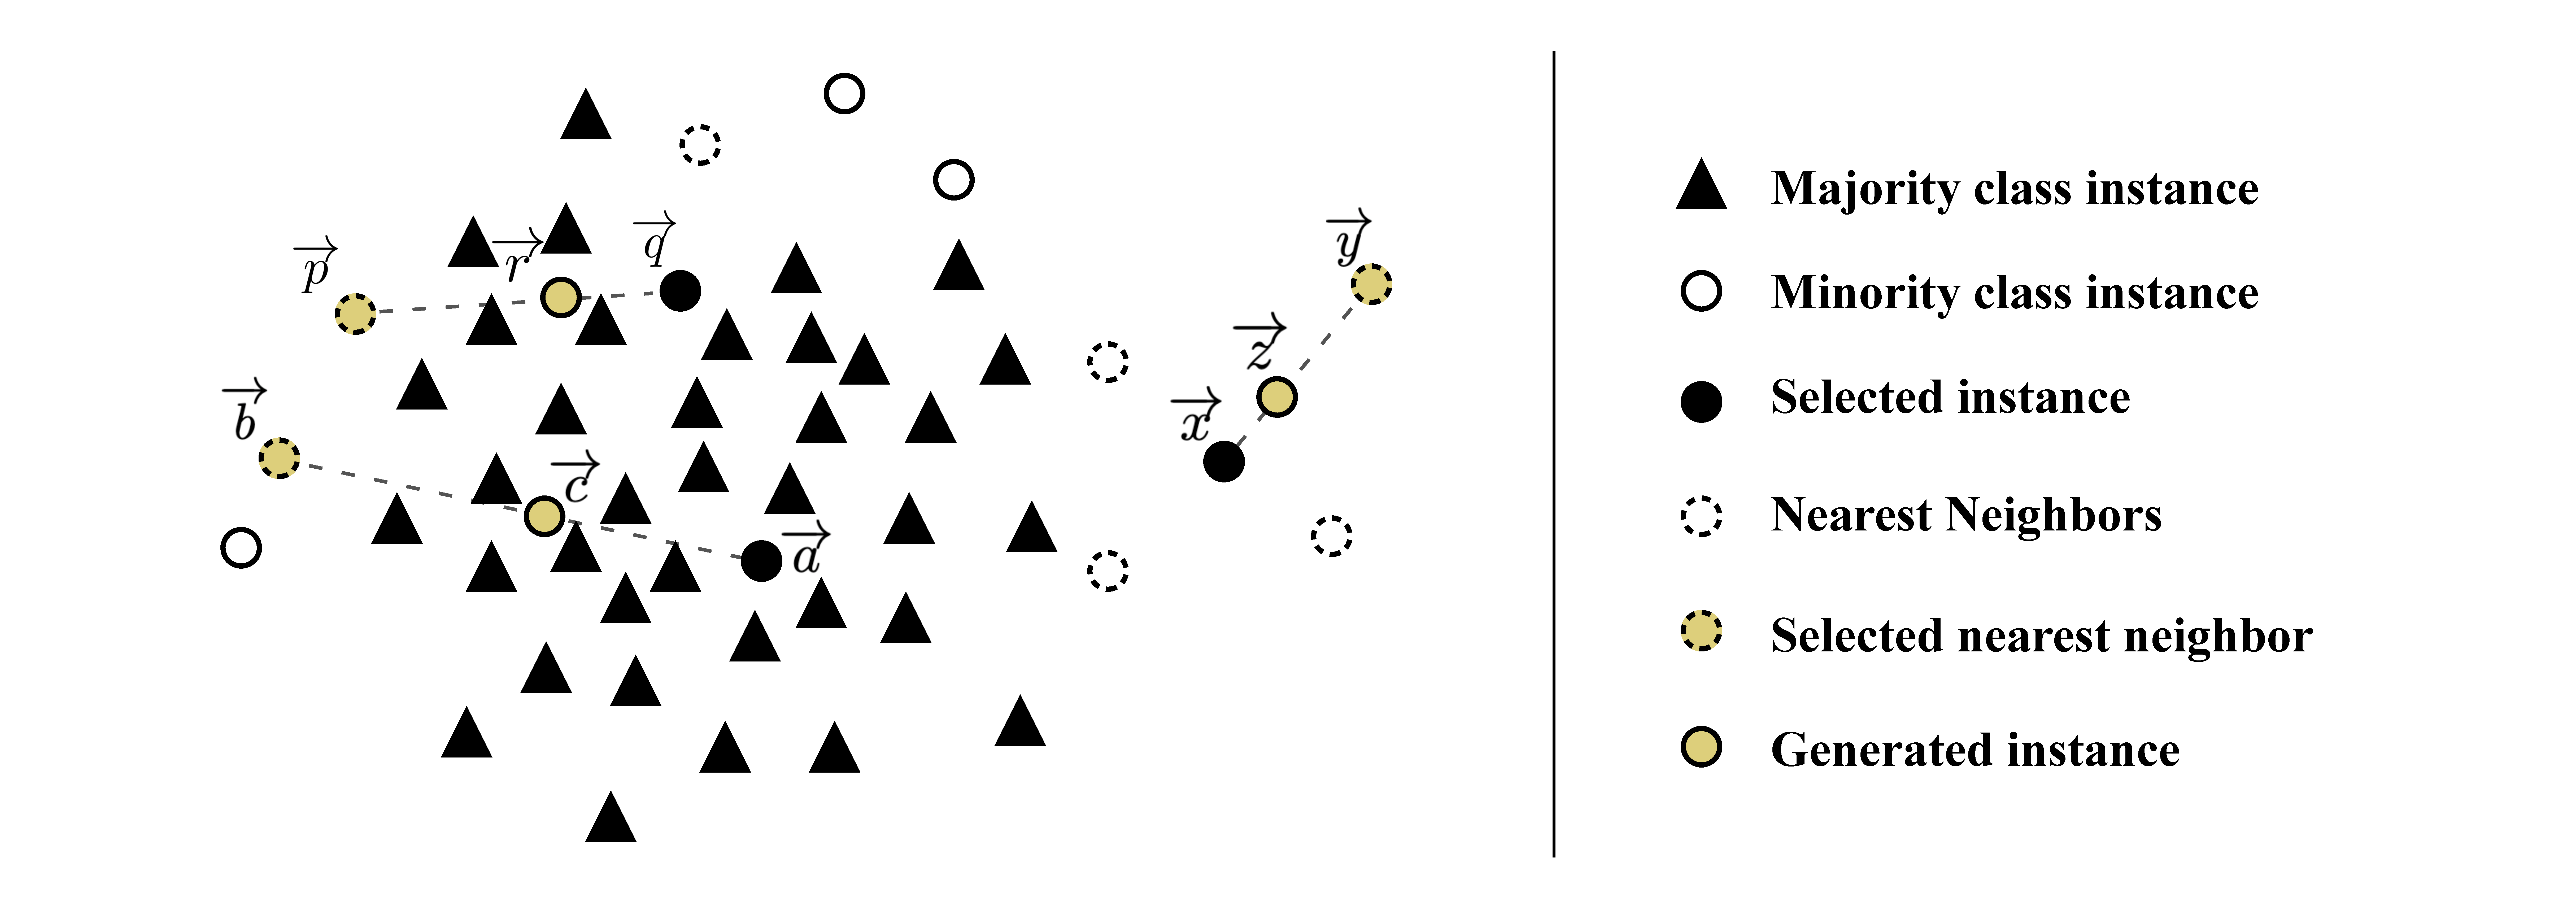
\includegraphics[width=1\linewidth]{smote_example}
    \caption[Example of SMOTE's data generation process]{Example of SMOTE's
        data generation process. SMOTE randomly selects instance
        $\protect\overrightarrow{x}$ and randomly selects one of its k-nearest
        neighbors $\protect\overrightarrow{y}$ to produce
        $\protect\overrightarrow{z}$.  Noisy instance
        $\protect\overrightarrow{r}$ was generated by randomly selecting
        $\protect\overrightarrow{q}$ and randomly selecting its nearest
        neighbor $\protect\overrightarrow{p}$ from a different minority class
        cluster. Noisy instance $\protect\overrightarrow{c}$ was generated by
        randomly selecting the noisy minority class instance
        $\protect\overrightarrow{a}$ and one of its nearest neighbors
        $\protect\overrightarrow{b}$.
    }~\label{fig:smote_example}
\end{figure}

A number of studies implement SMOTE within the LULC classification context and
reported improvements on the quality of the trained predictors
\cite{Jozdani2019, Bogner2018}. Another study proposes an adaptation of SMOTE
on an algorithmic level for deep learning applications \cite{Zhu2020}. This
method combines both typical computer vision data augmentation techniques,
such as image rotation, scaling and flipping on the generated instances to
populate minority classes. Another algorithmic implementation is the
variational semi-supervised learning model \cite{Cenggoro2018}. It consists of
a generative model that allows learning from both labeled and unlabeled
instances while using SMOTE to balance the data.

Despite SMOTE's popularity, its limitations have motivated the development of
more sophisticated oversampling algorithms \cite{Douzas2019, Han2005, Ma2017,
Douzas2017, Douzas2018, HaiboHe2008}. \cite{Douzas2019} identify four major
weaknesses of the SMOTE algorithm, which can be summarized as:

\begin{enumerate}
    \item Generation of noisy instances due to random selection of a
        minority instance to oversample. The random
        selection of a minority instance makes SMOTE
        oversampling prone to the amplification of existing noisy data. This
        has been addressed by variants such as B-SMOTE \cite{Han2005} and
        ADASYN \cite{HaiboHe2008}. 

    \item Generation of noisy instances due to the selection of the $k$
        nearest neighbors. In the event an instance
        (or a small number thereof) is not noisy but is isolated from the
        remaining clusters, known as the "small disjuncts problem"
        \cite{holte1989}, much like sample $\overrightarrow{b}$ from Figure
        \ref{fig:smote_example}, the selection of any nearest neighbor of the
        same class will have a high likelihood of producing a noisy sample.

    \item Generation of nearly duplicated instances. Whenever the linear
        interpolation is done between two instances that are close to each
        other, the generated instance becomes very similar to its parents and
        increases the risk of overfitting. G-SMOTE \cite{Douzas2019} attempts
        to address both the $k$ nearest neighbor selection mechanism problem
        as well as the generation of nearly duplicated instances problem. 

    \item Generation of noisy instances due to the use of
        instances from two different minority class clusters.
        Although an increased $k$ could potentially avoid the previous
        problem, it can also lead to the generation of artificial data between
        different minority clusters, as depicted Figure
        \ref{fig:smote_example} with the generation of point
        $\overrightarrow{r}$ using minority class instances $\overrightarrow{p}$ and $\overrightarrow{q}$.
        Cluster-based oversampling methods attempt to address this problem. 
\end{enumerate}

This last issue, the generation of noisy instances due to the existence of
several minority class clusters, is particularly relevant in remote sensing.
It is frequent that instances belonging to the same minority class can have
different spectral signatures, meaning that they will be clustered in
different parts of the input space. For example, in the classification of a
hyperspectral scene dominated by agricultural activities, patches relating to
urban areas may constitute a minority class. These patches frequently refer to
different types of land use, such as housing regions, small gardens, asphalt
roads, etc., all these containing different spectral signatures. In this
context, the use of SMOTE will lead to the generation of noisy instances of
the minority class. This problem can be efficiently mitigated through the use
of a cluster-based oversampling method. According to our literature review
cluster-based oversampling approaches have never been applied in the context
of remote sensing. On the other hand, while there are references of the
application of cluster-based oversampling in the context of machine
learning~\cite{Santos2015, Douzas2017, Ma2017, Douzas2018}, the multiclass
case is rarely addressed, which is a fundamental requirement for the
application of oversampling in the context of LULC. 

Cluster-based oversampling approaches introduce an additional layer to SMOTE's
selection mechanism, which is done through the inclusion of a clustering
process. This ensures that both between-class data balance and
within-class balance is preserved. The
self-organizing map oversampling (SOMO) \cite{Douzas2017} algorithm transforms
the dataset into a 2-dimensional input, where the areas with the highest
density of minority samples are identified. SMOTE is then used to oversample
each of the identified areas separately. ClUstered REsampling SMOTE
(CURE-SMOTE) \cite{Ma2017} applies a hierarchical clustering
algorithm to discard isolated minority instances before applying SMOTE.
Although it avoids noise generation problems, it ignores within-class data
distribution. Another method \cite{Santos2015} uses K-means to cluster the
entire input space and applies SMOTE to clusters with the fewest
instances, regardless of their class label. The label of the
generated instance is copied from one of its parents.
This method cannot ensure a balanced dataset since class imbalance is not
specifically addressed, but rather dataset imbalance.

\begin{figure}
	\centering
	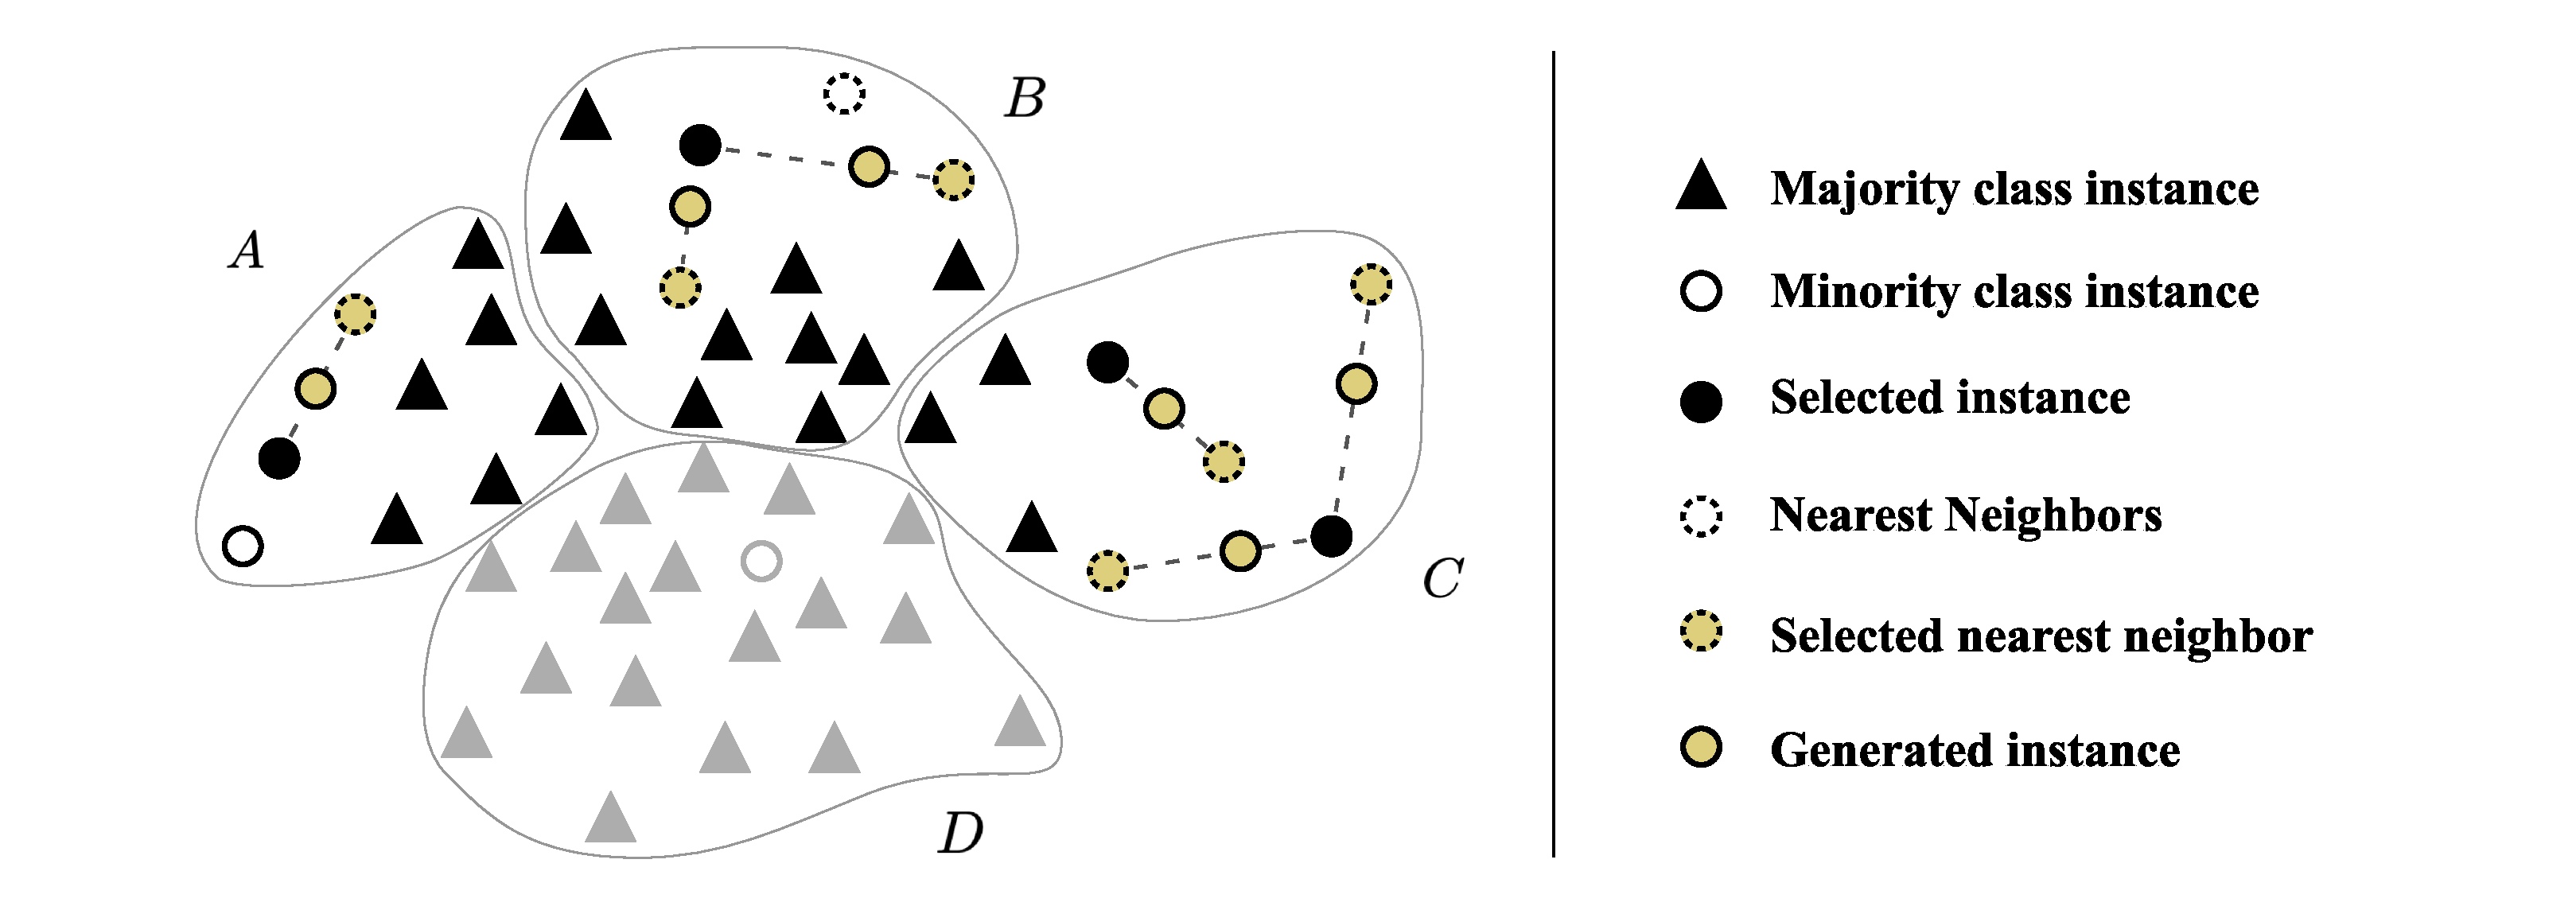
\includegraphics[width=1\linewidth]{kmeans_smote_example}
    \caption[Example of K-means SMOTE's data generation process.]{Example of
        K-means SMOTE's data generation process. Clusters $A$, $B$ and $C$ are
        selected for oversampling, whereas cluster $D$ was rejected due to its
        high imbalance ratio. The oversampling is done using the SMOTE
        algorithm and the $k$ nearest neighbors selection only considers
        instances within the same cluster.
    }~\label{fig:kmeans_smote_example}
\end{figure}

K-means SMOTE~\cite{Douzas2018} avoids noisy data generation by modifying the
data selection mechanism. It employs $k$-means clustering to identify safe
areas using cluster-specific Imbalance Ratio (IR, defined by
$\frac{count(C_{majority})}{count(C_{minority})}$) and determine the quantity
of generated samples per cluster based on a density measure. These samples are
finally generated using the SMOTE algorithm. The K-means SMOTE's data
generation process is depicted in Figure~\ref{fig:kmeans_smote_example}. Note
that the number of samples generated for each cluster varies according to the
sparsity of each cluster (the sparser the cluster is, the more samples will be
generated) and a cluster is rejected if the cluster's IR surpasses the
threshold.  Therefore, this method can be combined with any data generation
mechanism, such as G-SMOTE.  Also K-means SMOTE includes the SMOTE algorithm
as a special case when the number of clusters is set to one. Consequently,
K-means SMOTE returns results as good as or better than SMOTE.

Although no other study was found to implement cluster-based oversampling,
another study \cite{Douzas2019rs} compared the performance of SMOTE, ROS,
ADASYN, B-SMOTE and G-SMOTE in a highly imbalanced LULC classification dataset.
The authors found that G-SMOTE consistently outperformed the remaining
oversampling algorithms regardless of the classifier used.

\section{Methodology}\label{sec:methodology-kmeans}

The purpose of this work is to understand the performance of K-means SMOTE as
opposed to other popular and/or state-of-the-art oversamplers for LULC
classification. This is done using 7 datasets with predominantly land use
information, along with 3 evaluation metrics and 3 classifiers to evaluate the
performance of oversamplers. In this section we describe the datasets,
evaluation metrics, oversamplers, classifiers and software used as well as the
procedure developed.

\subsection{Datasets}

The datasets used were extracted from publicly available hyperspectral scenes.
Information regarding each of these scenes is provided in this subsection.
The data collection and preprocessing pipeline is shown in
Figure~\ref{fig:data_preprocessing_pipeline} and is common to all
hyperspectral scenes:

\begin{enumerate}
    
    \item Data collection of publicly available hyperspectral scenes.
        The original hyperspectral scenes and ground truth data were collected
        from a single publicly available data repository available
        \href{http://www.ehu.eus/ccwintco/index.php?title=Hyperspectral_Remote_Sensing_Scenes}{here}.

    \item Conversion of each hyperspectral scene to a structured
        dataset and removal of instances with no associated LULC class. This
        done to reshape the dataset from $(h,w,b+gt)$  into a conventional
        dataframe of shape $(h*w,b+gt)$, where $gt$, $h$, $w$ and $b$
        represents the ground truth, height, width and number of bands in the
        scene, respectively. The pixels without ground truth information are
        discarded from further analysis.

    \item Stratified random sampling to maintain similar class
        proportions on a sample of 10\% of each dataset. This is done by
        computing the relative class frequencies in the original hyperspectral
        scene (minus the class representing no ground truth availability) and
        retrieving a sample that ensures the original relative class
        frequencies remain unchanged.

    \item Removal of instances belonging to a class with frequency
        lower than 20 or higher than 1000. This is done to maintain the
        datasets to a practicable size due to computational constraints, while
        conserving the relative LULC class frequencies and data distribution. 

    \item Data normalization using the MinMax scaler. This ensures all
        features (i.e., bands) are in the same scale. In this case, the data
        was rescaled between 0 and 1.

\end{enumerate}

Table~\ref{tab:datasets_description_kmeans} provides a description of the final
datasets used for this work, sorted according to its IR.
Figure~\ref{fig:scenes_lulc} shows the original hyperspectral scene out of which
the dataset used in this experiment were extracted. In the representation of
the ground truth of these scenes, the blue regions in the ground truth of each
hyperspectral scene represent unlabeled regions (i.e., no  ground truth is
available). Particularly, in the Botswana and Kennedy Space Center scenes the
truth was photointerpreted in more limited regions of the scene. However, the
scenes are still represented as they are in order to maintain a standardized
analysis over all datasets extracted for the experiment.

\begin{figure}
	\centering
	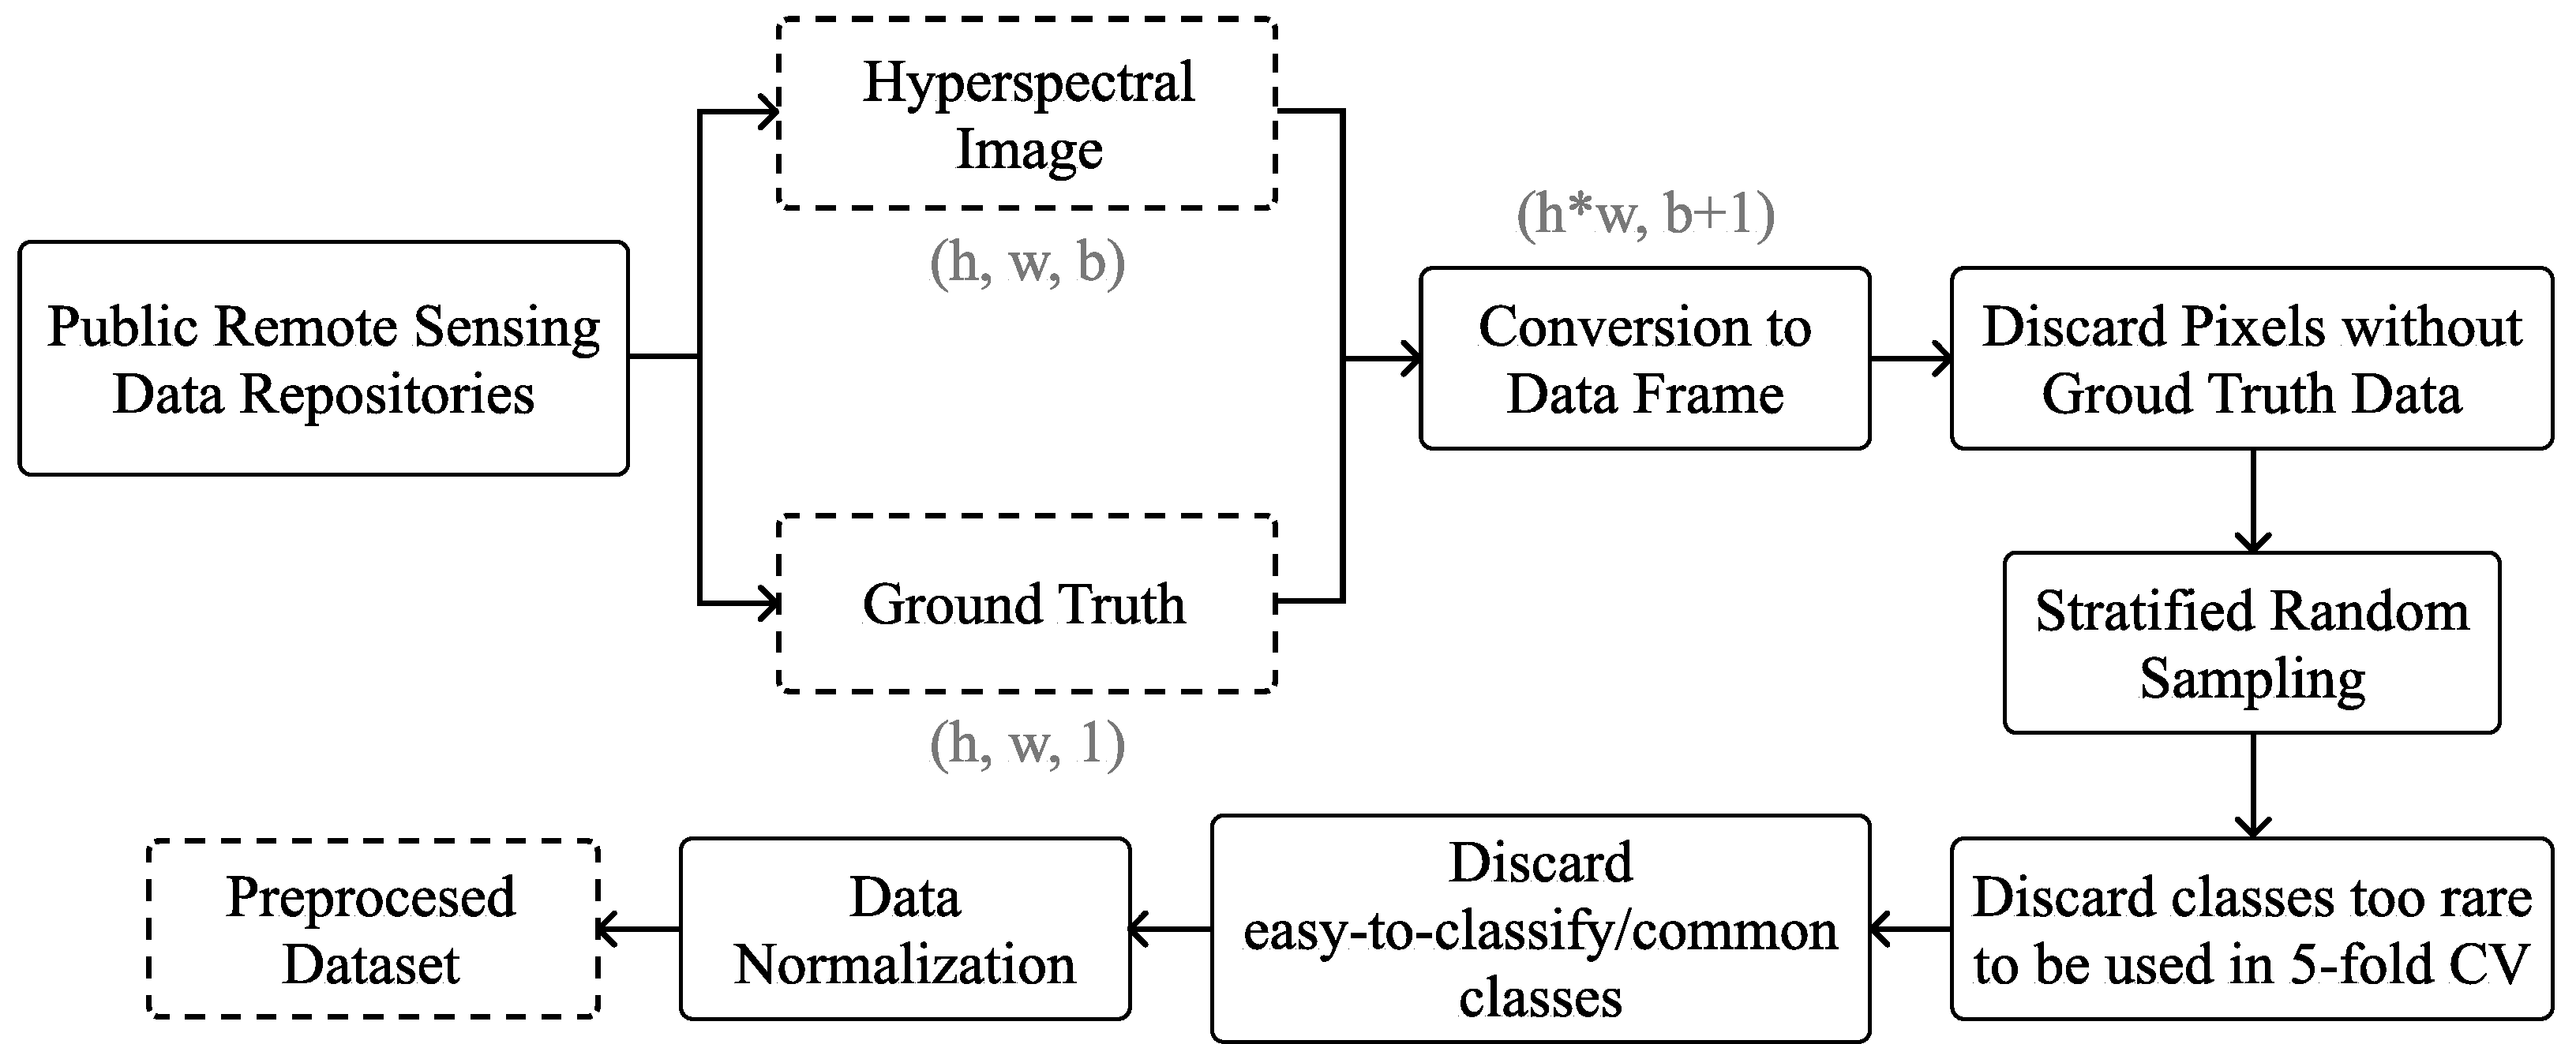
\includegraphics[width=.75\linewidth]{data_preprocessing_pipeline}
    \caption{Data collection and preprocessing
    pipeline.}~\label{fig:data_preprocessing_pipeline}
\end{figure}

\begin{table}
	\centering
    \addtolength{\leftskip} {-2cm}
    \addtolength{\rightskip}{-2cm}
    \pgfplotstabletypeset[
        col sep=comma,
        string type,
        every head row/.style={%
            before row=\toprule,
            after row=\midrule
        },
        every last row/.style={after row=\bottomrule},
        string type,
    ]{figures/kmeans-smote-lulc/datasets_description.csv}
    \caption{Description of the datasets used for this
    experiment.}~\label{tab:datasets_description_kmeans}
\end{table}

\subsubsection*{Botswana}

The Botswana scene was acquired by the Hyperion sensor on the NASA EO-1
satellite over the Okavango Delta, Botswana in 2001-2004 at a 30m spatial
resolution. Data preprocessing was performed by the UT Center for Space
Research. The scene comprises a $1476 \times 256$ pixels with 145 bands and 14
classes regarding land cover types in seasonal and occasional swamps, as well
as drier woodlands (see Figure~\ref{fig:botswana}). The classes with
rare instances are Short mopane and Hippo grass.

\subsubsection*{Pavia Center and University}

Both Pavia Center and University scenes were acquired by the ROSIS sensor.
These scenes are located in Pavia, northern Italy. Pavia Center is a $1096
\times 1096$ pixels image with 102 spectral bands, whereas Pavia University is
a $610 \times 610$ pixels image with 103 spectral bands. Both images have a
geometrical resolution of 1.3m and their ground truths are
composed of 9 classes each (see Figures~\ref{fig:pavia_center}
and~\ref{fig:pavia_university}). After data preprocessing, the classes
with rare instances are Asphalt and Bitumen (the class Shadows was removed for
being too rare for cross validation after random sampling).

\subsubsection*{Kennedy Space Center}

The Kennedy Space Center scene was acquired by the AVIRIS sensor over the
Kennedy Space Center, Florida, on March 23, 1996. Out of the original 224
bands, water absorption and low SNR bands were removed and a total of 176
bands at a spatial resolution of 18m are used. The scene is a $512 \times 614$
pixel image and contains a total of 16 classes (see
figure~\ref{fig:kennedy_space_center}). The classes with rare instances
are hardwood swamp, slash pine and willow swamp (both hardwood swamp and slash
pine were removed for being too rare for cross validation after random
sampling).

\subsubsection*{Salinas and Salinas-A}

These scenes were collected by the AVIRIS sensor over Salinas Valley,
California and contain at-sensor radiance data. Salinas is a $512 \times 217$
pixels image with 224 bands and 16 classes regarding vegetables, bare soil and
vineyard fields (see Figure~\ref{fig:salinas}). Salinas-A, a subscene of
Salinas, comprises $86 \times 83$ pixels and contains 6 classes regarding
vegetables (see Figure~\ref{fig:salinas_a}). These scenes have a geometrical
resolution of 3.7m. Salinas-A's minority class has the label
``Brocoli\_green\_weeds\_1'' and Salina's minority class has the label
``Lettuce\_romaine\_6wk''

\subsubsection*{Indian Pines} 

The Indian Pines scene~\cite{Baumgardner2015} was collected on June 12, 1992
and consists of AVIRIS hyperspectral image data covering the Indian Pine Test
Site 3, located in North-western Indiana, USA. As a subset of a larger scene,
it is composed of $145 \times 145$ pixels (see Figure~\ref{fig:indian_pines})
and 220 spectral reflectance bands in the wavelength range 400 to 2500
nanometers at a spatial resolution of 20m. Approximately two thirds of
this scene is composed by agriculture and the other third is composed of
forest and other natural perennial vegetation. Additionally, the scene also
contains low density buildup areas. The classes with rare instances are
Alfalfa, Oats, Grass-pasture-mowed, Wheat and Stone-Steel-Towers (which
removed for being too rare for cross validation after random sampling).  After
data preprocessing, the classes with rare instances are Corn,
Buildings-Grass-Trees-Drives and Grass-Pasture.

\begin{figure}
	\centering
	\begin{subfigure}{.24\textwidth}
		\centering
		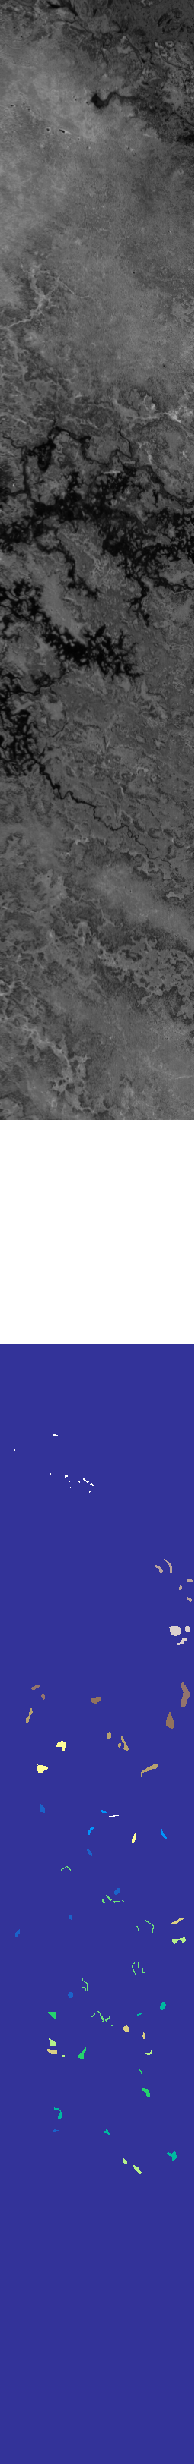
\includegraphics[height=1.5\linewidth]{botswana}
		\subcaption{{\medbreak}}\label{fig:botswana}
	\end{subfigure}
	\begin{subfigure}{.24\textwidth}
		\centering
		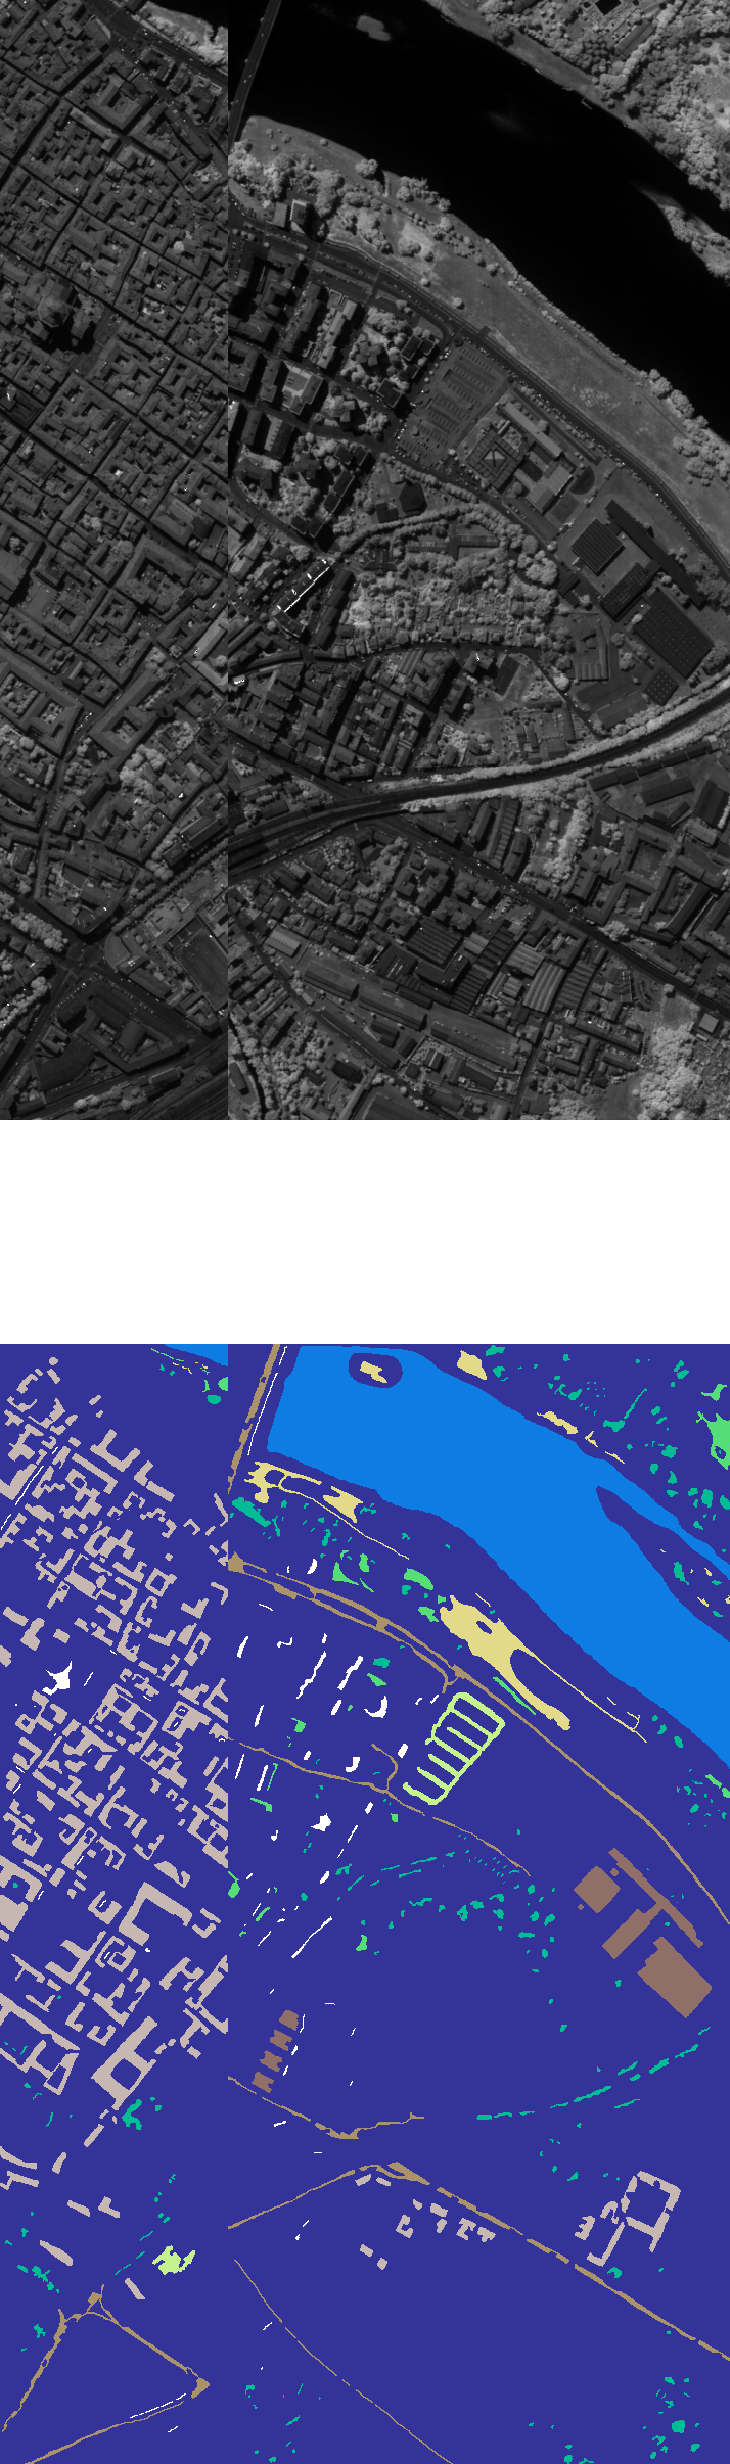
\includegraphics[height=1.5\linewidth]{pavia_centre}
		\subcaption{{\medbreak}}\label{fig:pavia_center}
	\end{subfigure}
	\begin{subfigure}{.24\textwidth}
		\centering
		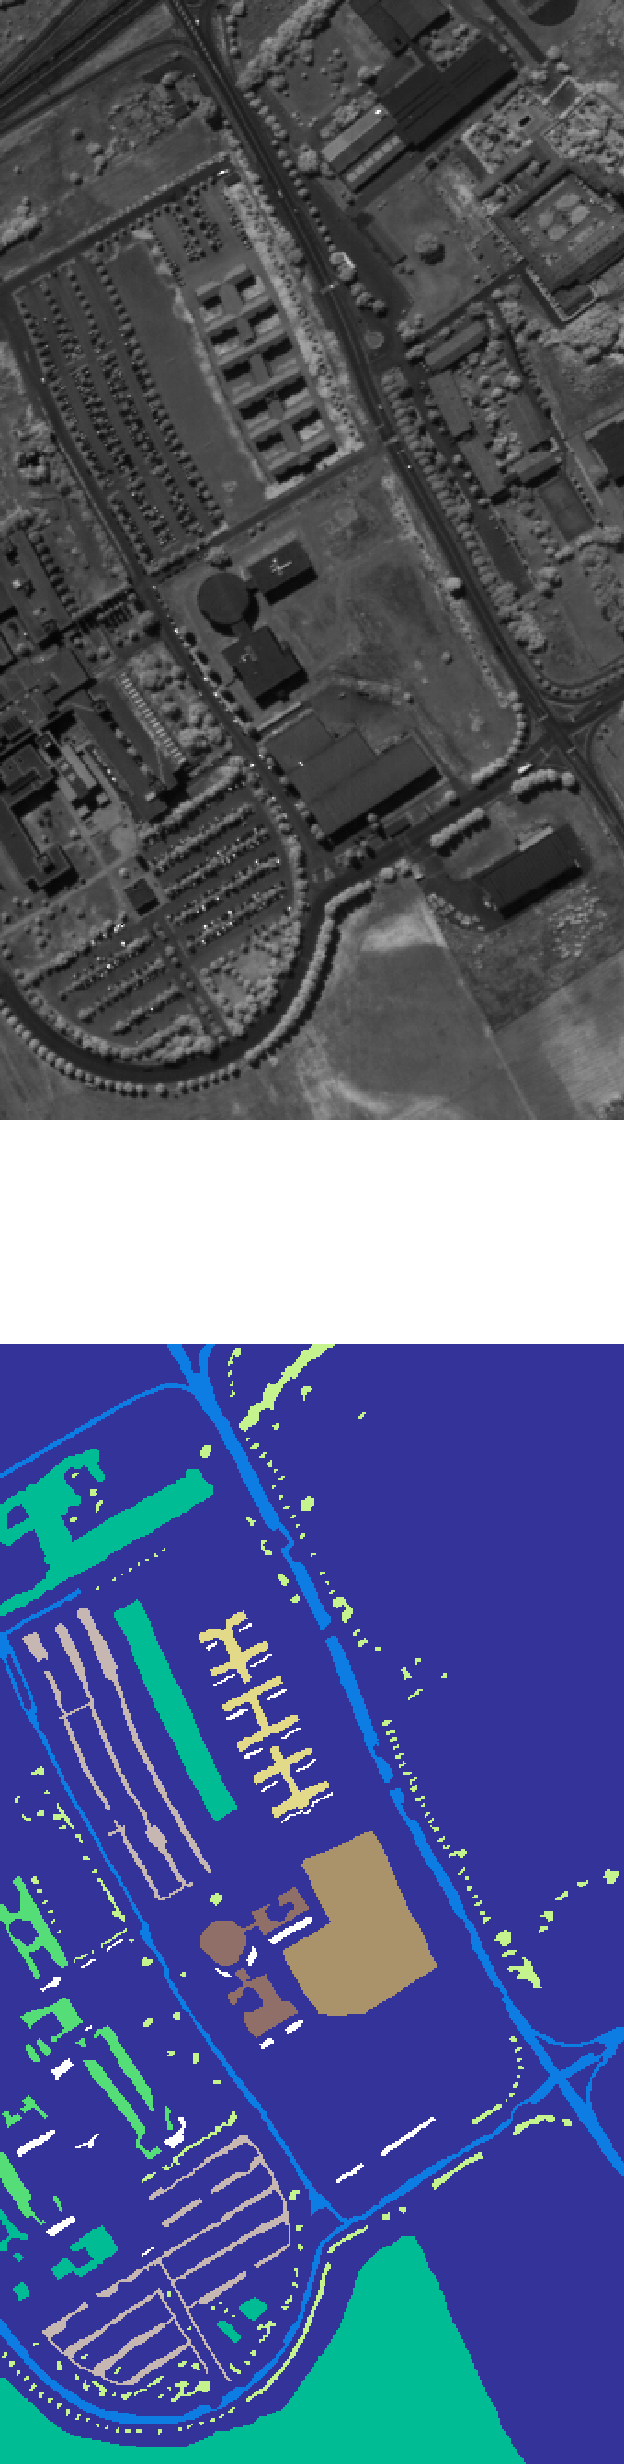
\includegraphics[height=1.5\linewidth]{pavia_university}
		\subcaption{{\medbreak}}\label{fig:pavia_university}
	\end{subfigure}
	\begin{subfigure}{.24\textwidth}
		\centering
		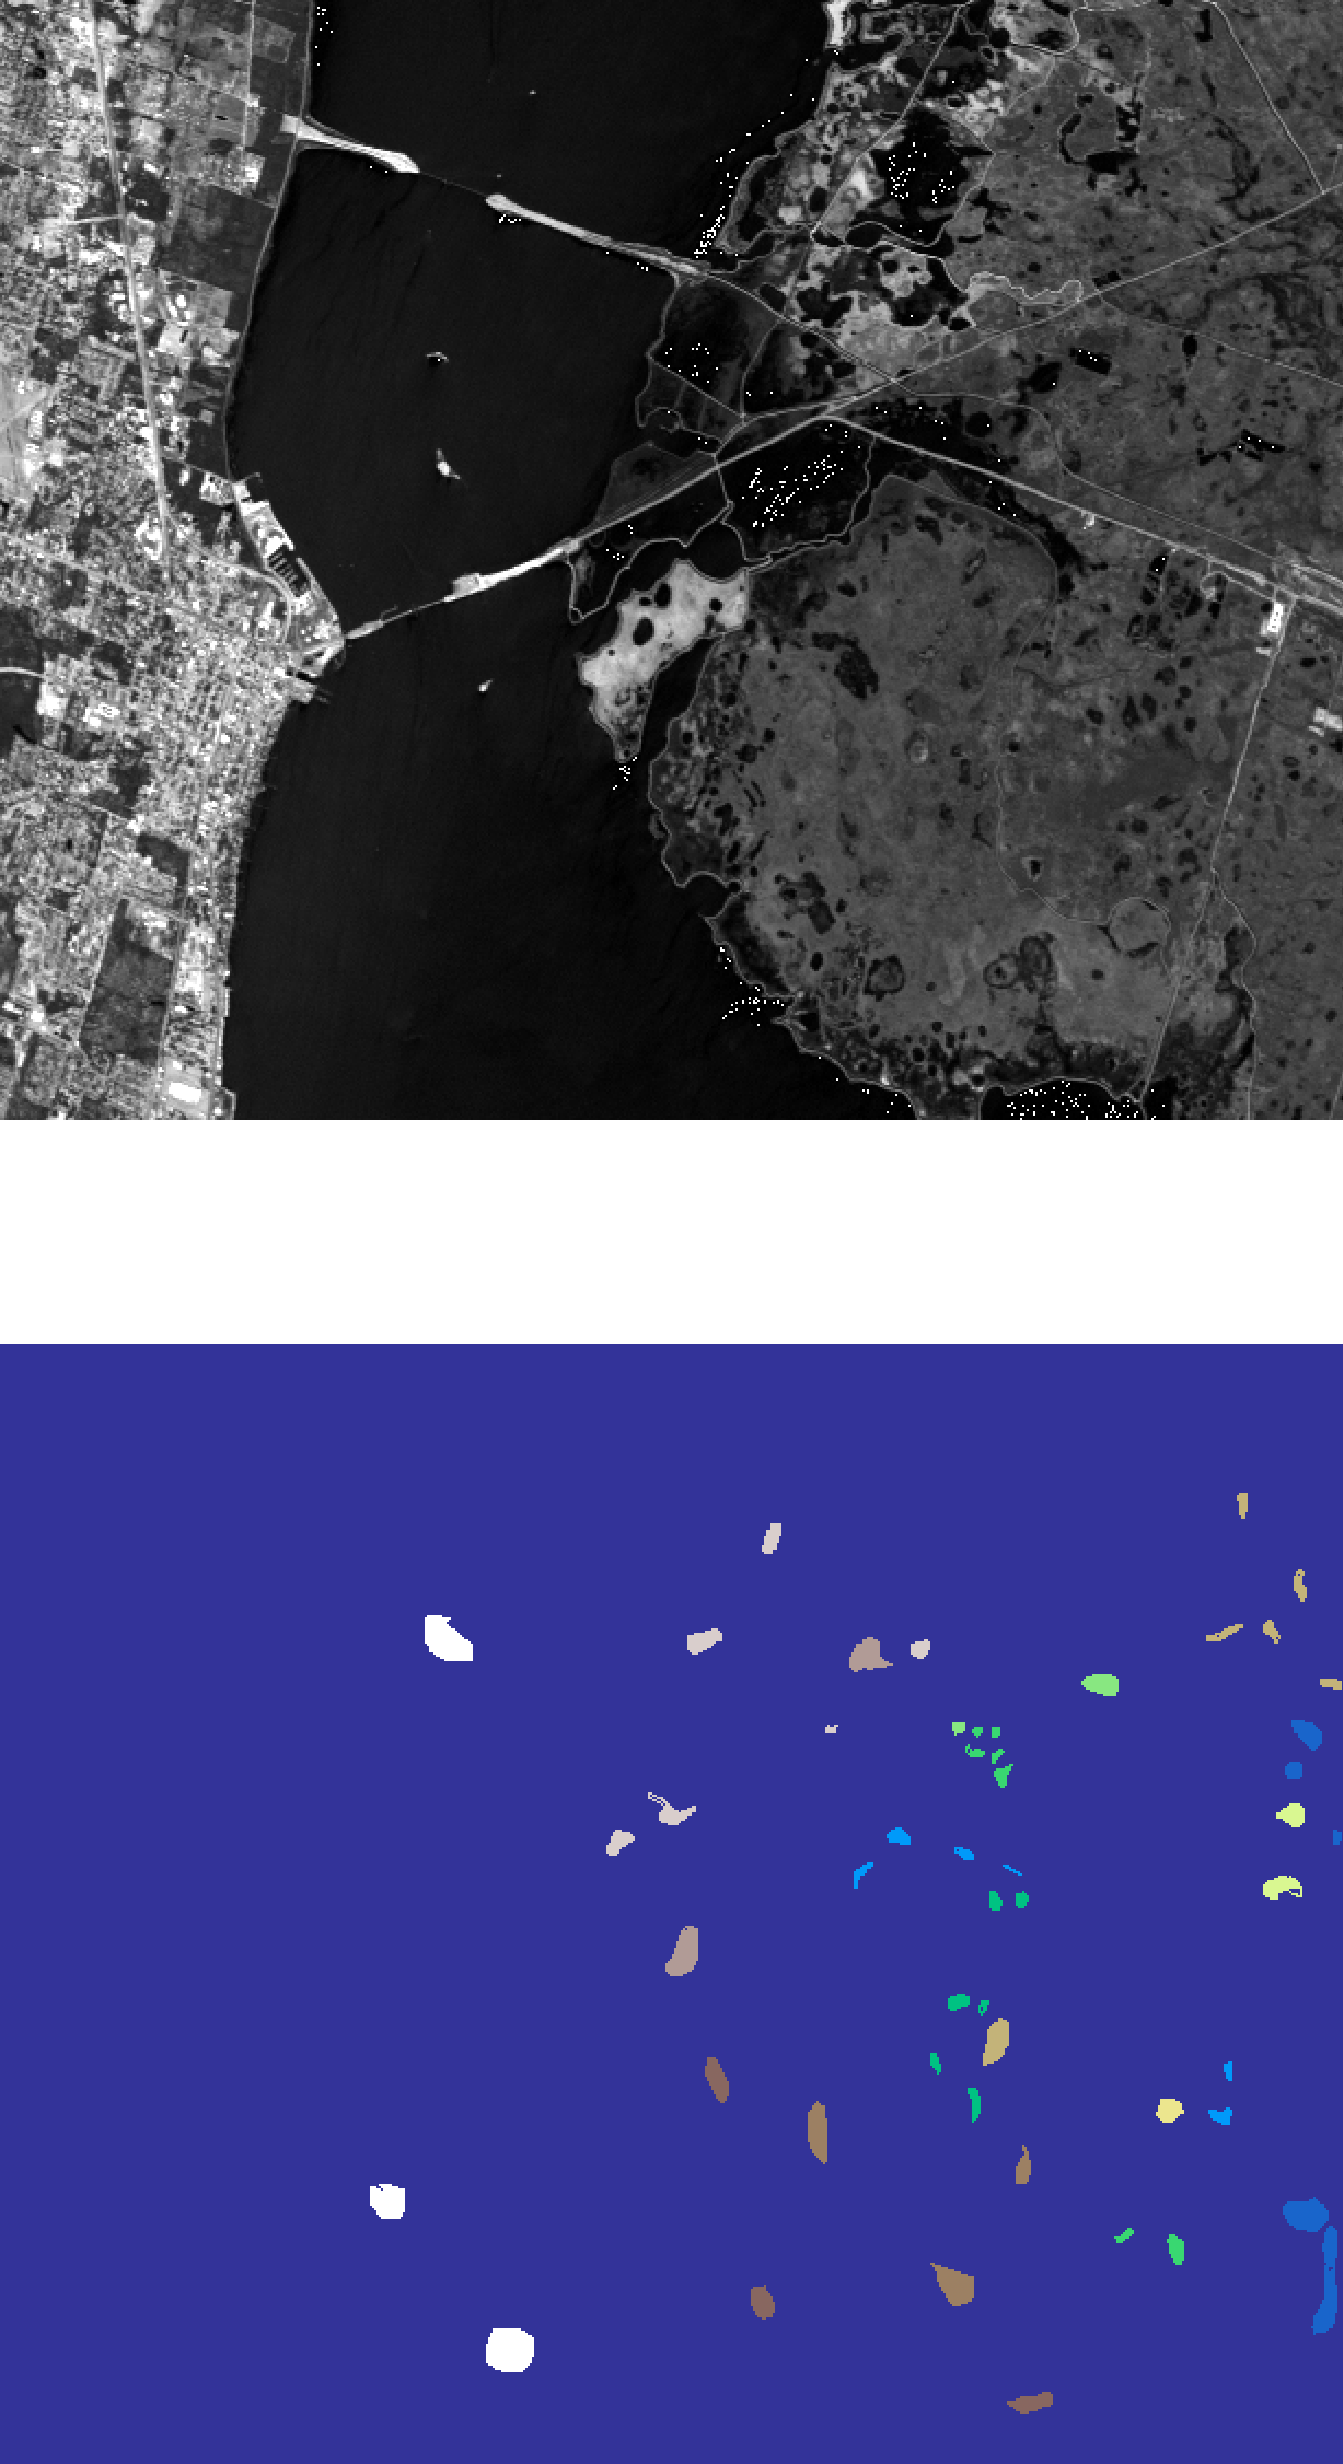
\includegraphics[height=1.5\linewidth]{kennedy_space_center}
		\subcaption{{\medbreak}}\label{fig:kennedy_space_center}
	\end{subfigure}

	\begin{subfigure}{.24\textwidth}
		\centering
		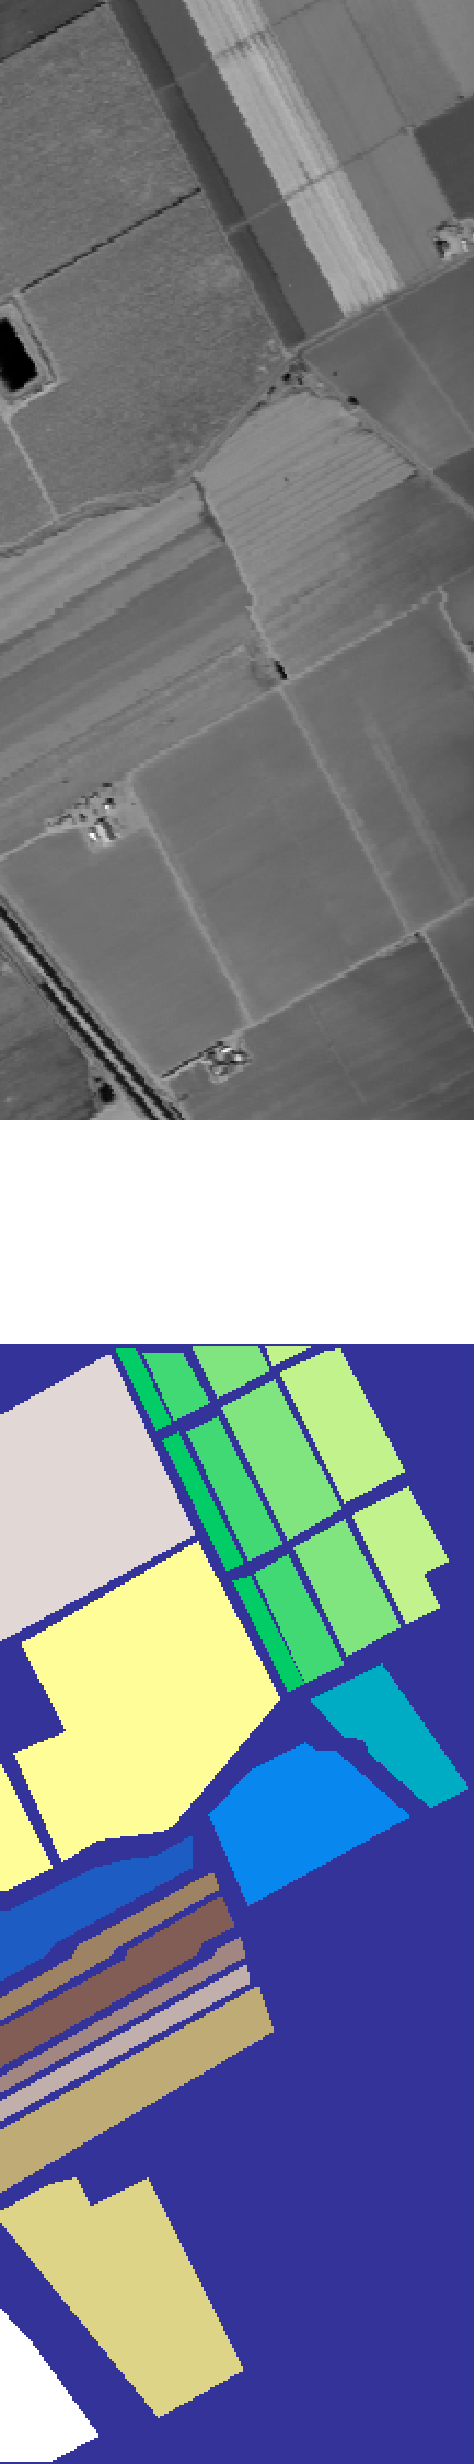
\includegraphics[height=1.5\linewidth]{salinas}
		\subcaption{{\medbreak}}\label{fig:salinas}
	\end{subfigure}
	\begin{subfigure}{.24\textwidth}
		\centering
		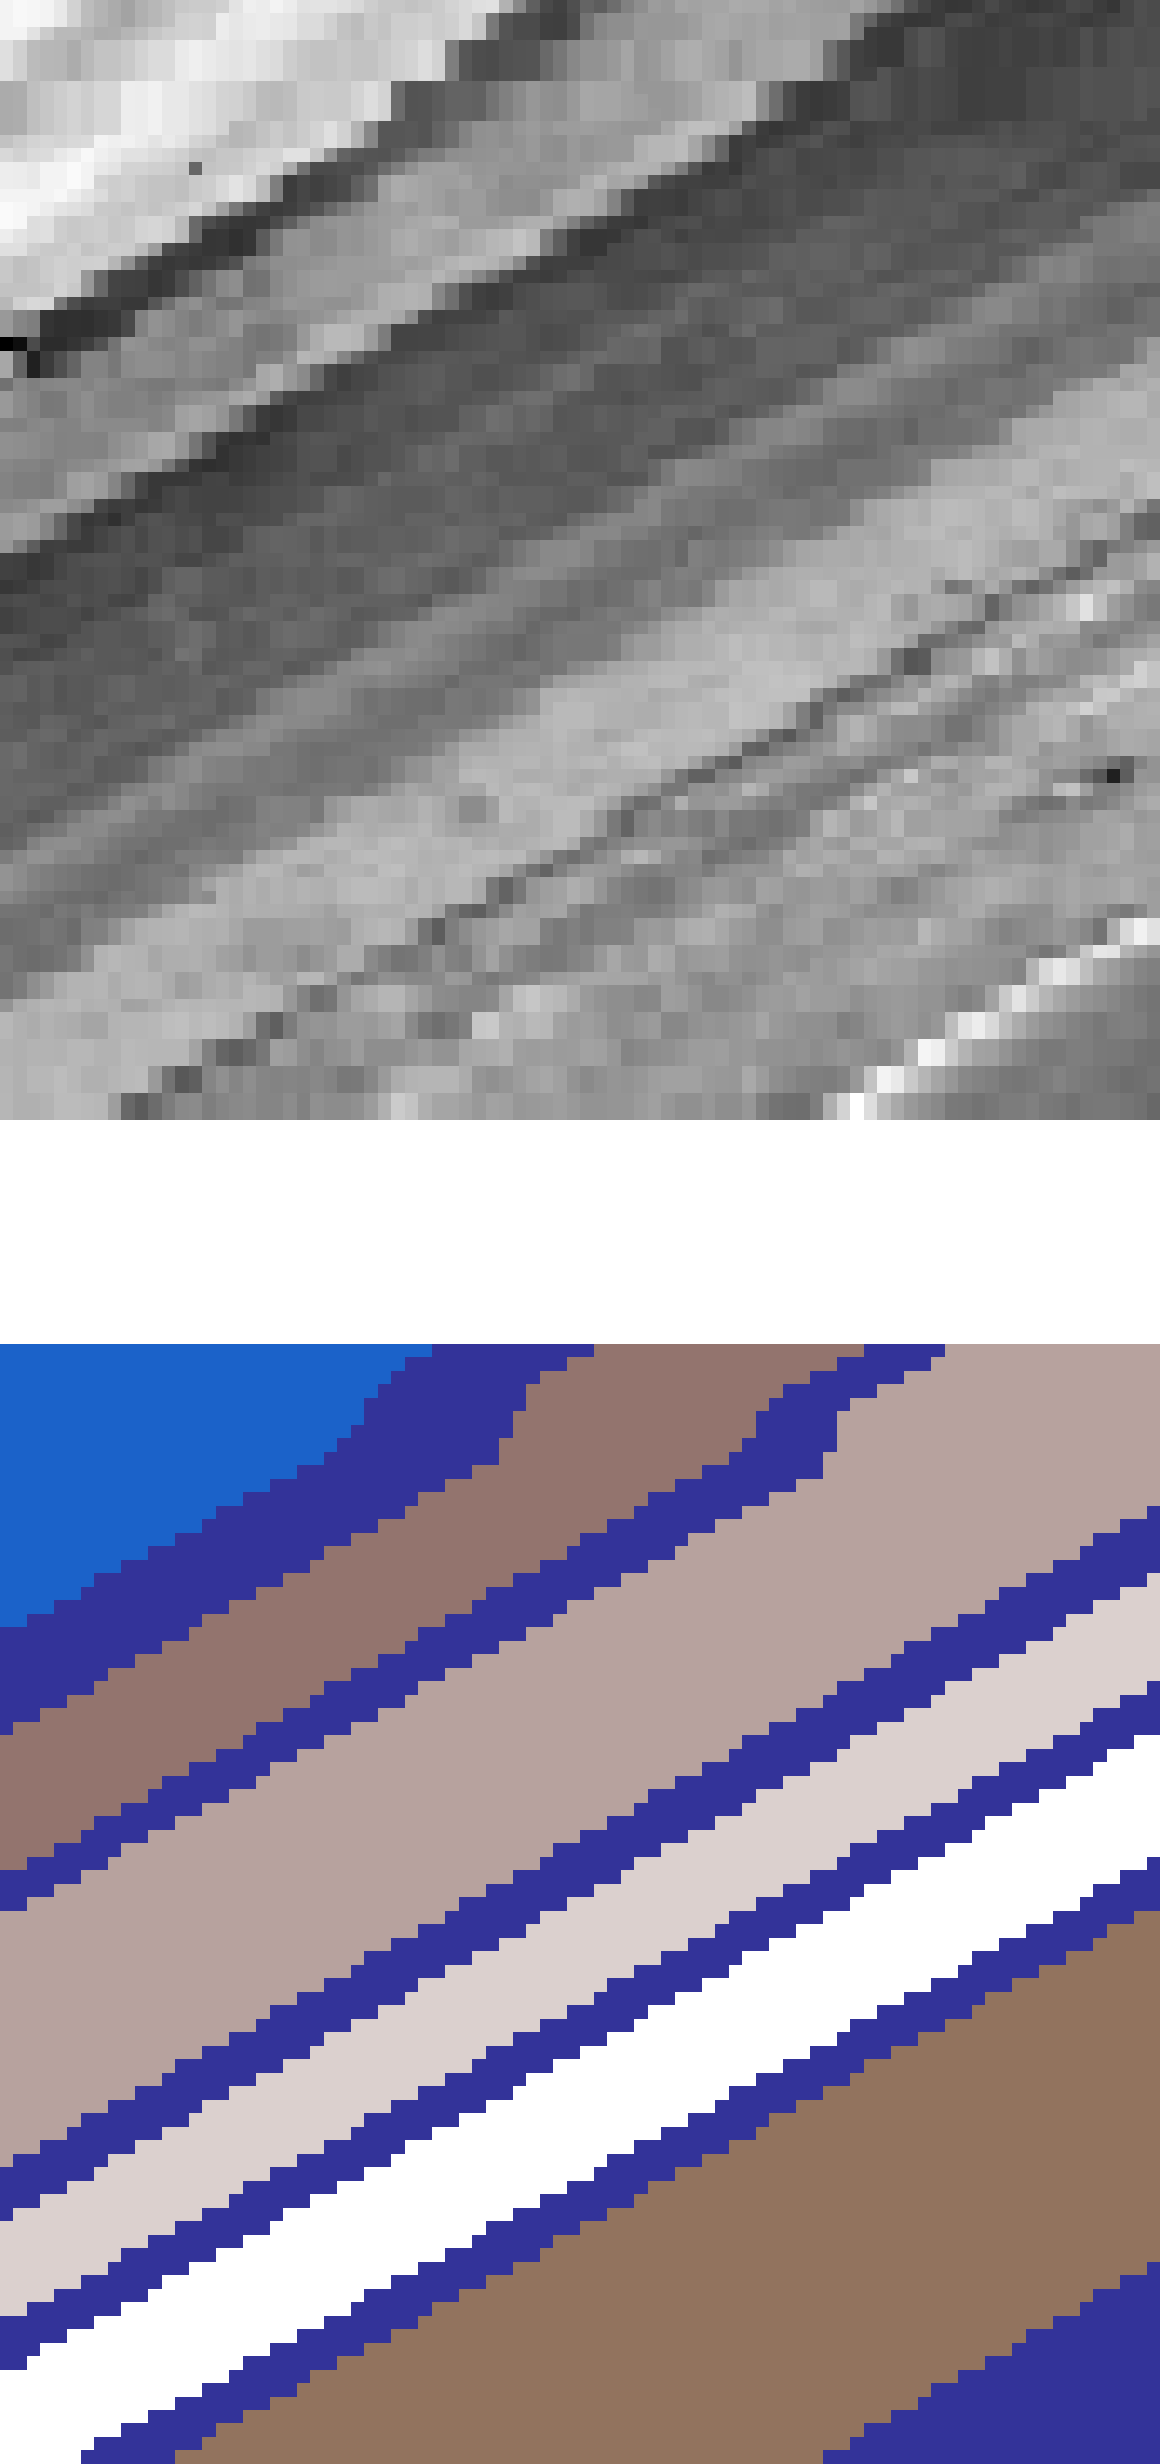
\includegraphics[height=1.5\linewidth]{salinas_a}
		\subcaption{{\medbreak}}\label{fig:salinas_a}
	\end{subfigure}
    \begin{subfigure}{.24\textwidth}
		\centering
		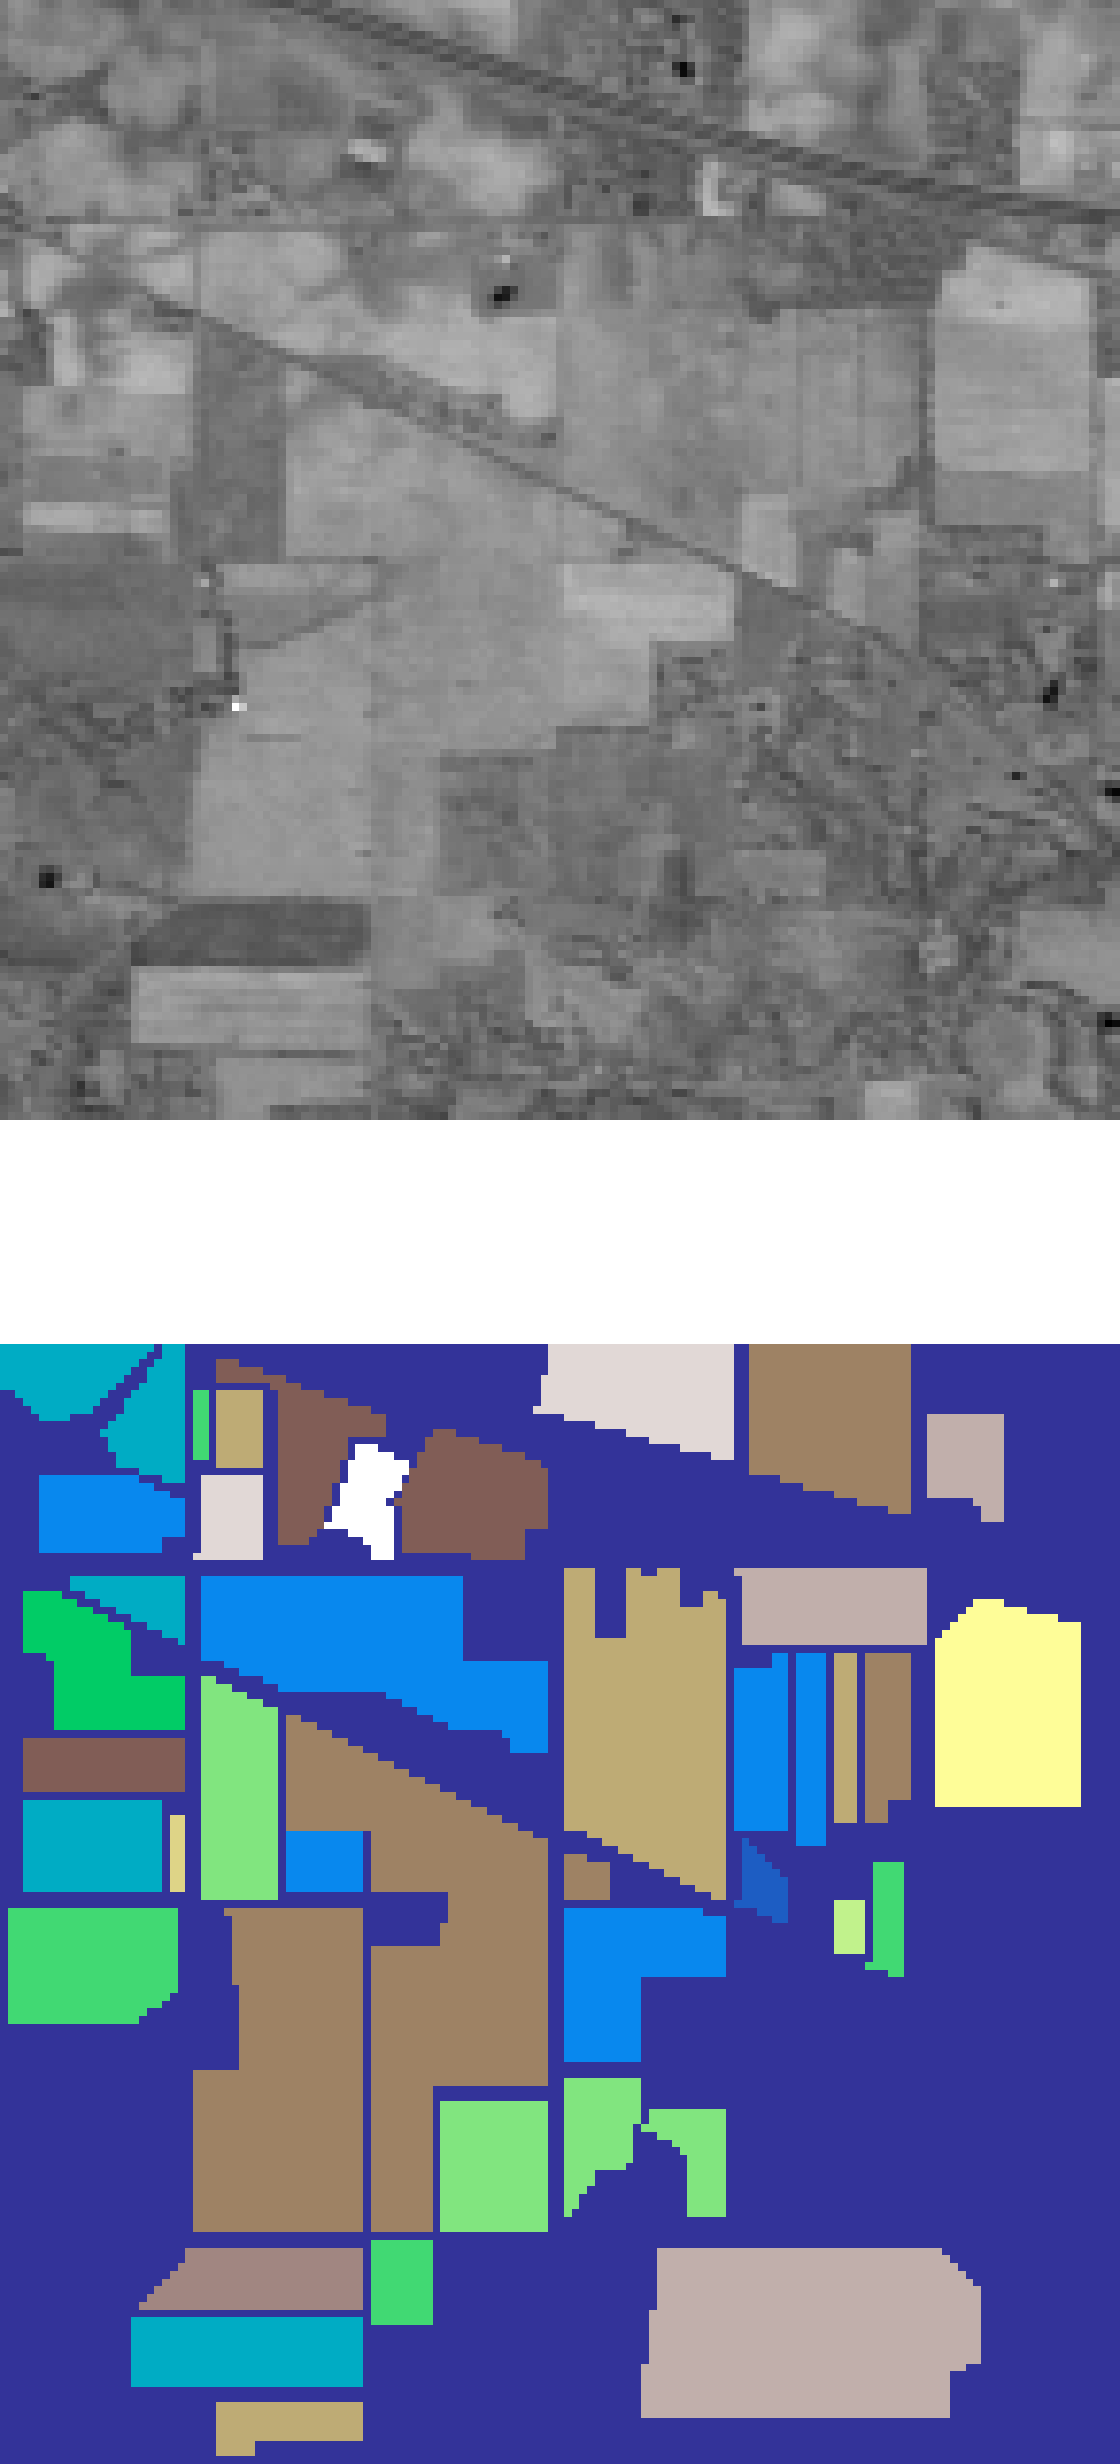
\includegraphics[height=1.5\linewidth]{indian_pines}
		\subcaption{{\medbreak}}\label{fig:indian_pines}
	\end{subfigure}
    \caption[Gray scale visualization of a band and ground truth
    of each scene used in this study.]{Gray scale visualization of a band (top
        row) and ground truth (bottom row) of each scene used in this study.
        (a) Botswana, (b) Pavia Center, (c) Pavia University, (d) Kennedy
        Space Center, (e) Salinas, (f) Salinas A, (g) Indian Pines.
    }~\label{fig:scenes_lulc}
	
\end{figure}

\subsection{Machine Learning Algorithms}

To assess the quality of the K-means SMOTE algorithm,
three other oversampling algorithms were used for benchmarking. ROS and SMOTE
were chosen for their simplicity and popularity. B-SMOTE chosen as a popular
variation of the SMOTE algorithm. We also include the classification results
of no oversampling (NONE) as a baseline.

To assess the performance of each oversampler, we use the classifiers Logistic
Regression (LR) \cite{Nelder1972}, K-Nearest Neighbors (KNN)
\cite{Cover1967} and Random Forest (RF)
\cite{Liaw2002}. This choice was based on the classifiers' popularity for LULC
classification, learning type and training time
\cite{Maxwell2018,Gavade2019}. Since this is a multinomial classification
task, for the LR classification we adopted a one-versus-all approach for each
label. The predicted label is assigned according to the class predicted with
highest probability.

\subsection{Evaluation Metrics}~\label{sec:evaluation-metrics-kmeans}

Most of the satellite-based LULC classification studies (nearly 80\%) employ
\textit{Overall Accuracy} (OA) and the \textit{Kappa Coefficient}
\cite{Gavade2019}. Although, some authors argue that both evaluation metrics,
even when used simultaneously, are insufficient to fully address the area
estimation and uncertainty information needs \cite{Olofsson2013,Pontius2011}.
Other metrics like User's Accuracy (or \textit{Precision}) and Producer's
Accuracy (or \textit{Recall}) are also common metrics to evaluate per-class
prediction power. These metrics consist of ratios employing the True and False
Positives (\textit{TP} and \textit{FP}, number of correctly/incorrectly
classified instances of a given class) and True and
False Negatives (\textit{TN} and \textit{FN}, number of correctly/incorrectly
classified instances as not belonging to a given
class). These metrics are formulated as $Precision = \frac{TP}{TP+FP}$ and
$Recall = \frac{TP}{TP+FN}$. While metrics like OA and \textit{Kappa
Coefficient} are significantly affected by imbalanced class distributions,
\textit{F-Score} is less sensitive to data imbalance and a more appropriate
choice for performance evaluation \cite{Jeni2013}.

The datasets used present significantly high IRs (see Table
\ref{tab:datasets_description_kmeans}). Therefore, it is especially important to
attribute equal importance to the predictive power of all classes, which does
not happen with OA and \textit{Kappa Coefficient}. In this study, we employ 3
evaluation metrics: 1) \textit{G-mean}, since it is not affected by skewed class
distributions, 2) \textit{F-Score}, as it proved to be a more appropriate metric
for this problem when compared to other commonly used metrics \cite{Jeni2013},
and 3) \textit{Overall Accuracy}, for discussion purposes.

\begin{itemize}
    \item The \textit{G-mean} consists of the geometric mean of $Specificity =
        \frac{TN}{TN + FP}$ and \textit{Sensitivity} (also known as
        \textit{Recall}). For multiclass problems, The \textit{G-mean} is
        expressed as:

        $$\textit{G-mean} = \sqrt{ \overline{Sensitivity} \times
        \overline{Specificity}}$$

    \item \textit{F-score} is the harmonic mean of \textit{Precision} and
        \textit{Recall}. The \textit{F-score} for the multi-class case can be
        calculated using their average per class values \cite{He2009}:

          $$\textit{F-score}=2\frac{\overline{Precision} \times
          \overline{Recall}}{\overline{Precision} + \overline{Recall}}$$

    \item \textit{Overall Accuracy} is the number of correctly classified
        instances divided by the total amount of instances. Having \( c \) as
        the label of the various classes, \textit{Accuracy} is given by the
        following formula:

          $$\textit{Accuracy} = \frac{ \sum\limits_{c}{ \text{TP}_{c} } }{
          \sum\limits_{c}{ (\text{TP}_{c}  + \text{FP}_{c}) } } $$

\end{itemize}

In the case of \textit{G-mean} and \textit{F-score}, both metrics are computed
for each label and their unweighted mean is calculated (\textit{i.e.},
following a ``macro'' approach). In this study we assume that all labels
have an equivalent importance for the classification task.

\subsection{Experimental Procedure}

The procedure for the experiment started with the definition of a
hyperparameter search grid, where a list of possible values for each relevant
hyperparameter in both classifiers and oversamplers is stored. Based on this
search grid, all possible combinations of oversamplers, classifiers and
hyperparameters are formed.  Finally, for each dataset, hyperparameter
combination and initialization we use the evaluation strategy shown in Figure
\ref{fig:experiment_pipeline}: $k$-fold cross-validation strategy where $k=5$
to train each model defined and save the averaged scores of each split.

In the 5-fold cross validation strategy, a combination
of oversampler, classifier and hyperparameters vector is fit 5 times
per dataset. Before the training
phase, the training set
(containing $\frac{4}{5}$ of the dataset) is oversampled using one of the methods
described (except for the baseline method NONE), creating an augmented
dataset with the exact same number of instances for
each class. The newly formed training dataset is used to train the classifier
and the test set ($\frac{1}{5}$ of the dataset)
is used to evaluate the performance of the classifier. The evaluation scores
are then averaged over the 5 times the process is repeated. The range of
hyperparameters used are shown in table \ref{tab:grid_kmeans}. The definition of
hyperparameters for the K-means SMOTE oversampler is defined according to the
recommendations discussed in the original K-means SMOTE
paper~\cite{Douzas2018}.

\begin{figure}
	\centering
	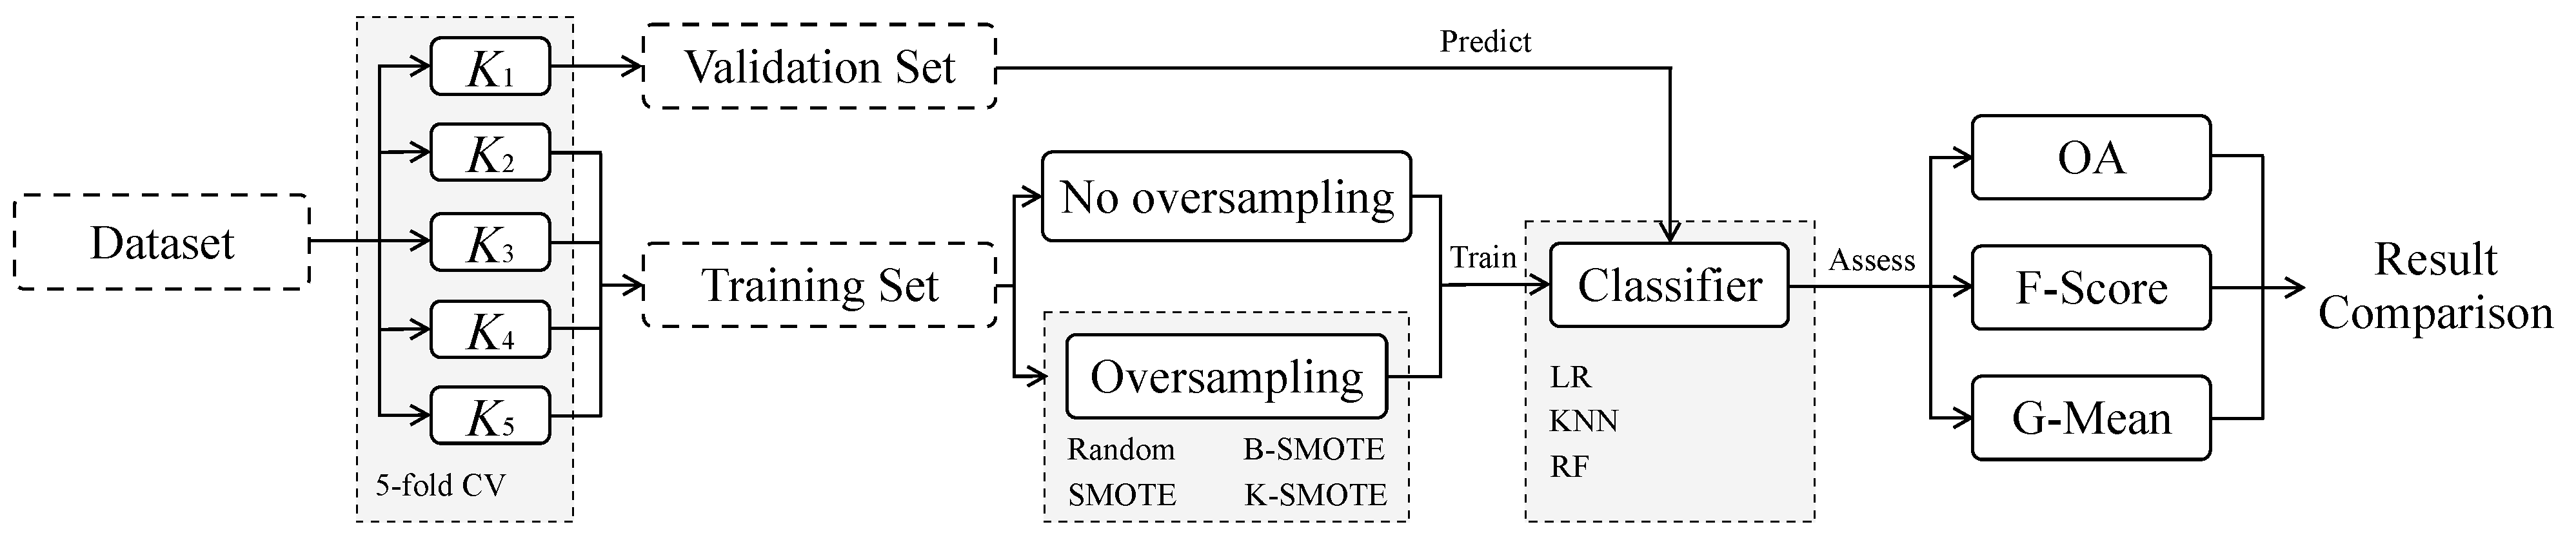
\includegraphics[width=1\linewidth]{experiment_pipeline}
    \caption[Experimental procedure.]{Experimental procedure. The performance metrics are averaged over
        the 5 folds across each of the 3 different initializations of this
        procedure for a given combination of oversampler, classifier and
        hyperparameter definition.
    }~\label{fig:experiment_pipeline}
\end{figure}

\begin{table}
	\centering
    \begin{tabular}{lll}
		\toprule
		Classifier       & Hyperparameters      & Values                            \\
		\midrule
		LR               & maximum iterations   & 10000                             \\
		KNN              & \# neighbors  & {3, 5, 8}                            \\
		RF               & maximum depth        & {None, 3, 6}                      \\
		                 & \# estimators & {50, 100, 200}                         \\
		\toprule
		Oversampler      &                      &                                   \\
		\midrule
        K-means SMOTE    & \# neighbors  & {3, 5}                            \\
		                 & \# clusters (as \% of number of instances)   & {1$^*$, 0.1, 0.3, 0.5, 0.7, 0.9}      \\
                         & Exponent of mean distance & {auto, 2, 5, 7}       \\
                         & IR threshold  & {auto, 0.5, 0.75, 1.0}            \\
		SMOTE            & \# neighbors  & {3, 5}                            \\
		BORDERLINE SMOTE & \# neighbors  & {3, 5}                            \\
		\bottomrule
	\end{tabular}
    \caption[Hyper-parameters grid.]{Hyper-parameters grid. $^*$~One cluster is generated in total, a
    corner case that mimics the behavior of SMOTE
    }\label{tab:grid_kmeans}
\end{table}

\subsection{Software Implementation}~\label{sec:implementation-kmeans}

The experiment was implemented using the Python programming language, using the
\href{https://scikit-learn.org/stable/}{Scikit-Learn}~\cite{Pedregosa2011},
\href{https://imbalanced-learn.org/en/stable/}{Imbalanced-Learn}~\cite{JMLR:v18:16-365},
\href{https://geometric-smote.readthedocs.io/en/latest/?badge=latest}{Geometric-SMOTE},
\href{https://cluster-over-sampling.readthedocs.io/en/latest/?badge=latest}{Cluster-Over-Sampling}
and \href{https://research-learn.readthedocs.io/en/latest/?badge=latest}{Research-Learn} libraries.
All functions, algorithms, experiments and results are provided at the
\href{https://github.com/joaopfonseca/publications}{GitHub
repository of the project}.

\section{Results \& Discussion}~\label{sec:results-kmeans}

When evaluating the performance of an algorithm across multiple datasets, it
is generally recommended to avoid direct score comparisons and use
classification rankings instead~\cite{Demsar2006}. This is done by assigning
a ranking to oversamplers based on the different combinations of classifier,
metric and dataset used. These rankings are also used for the statistical
analyses presented in Section~\ref{sec:statistical_analysis-kmeans}.

The rank values are assigned based on the mean validation scores resulting
from the experiment described in Section~\ref{sec:methodology-kmeans}. The averaged
ranking results are computed over 3 different initialization seeds and a 5
fold cross validation scheme, returning a real number within the interval
$[1,5]$.

The hyperparameter optimization ensures that both oversamplers and classifiers
are well adapted to each of the datasets used in the experiment. Specifically,
the optimization of classifiers' hyperparameters is not particularly relevant
since our focus is to study the relative performance scores across
oversamplers. This will provide insights on the quality of the artificial data
generated by each oversampler. The classifiers' hyperparameter tuning was done
to avoid the over/underfitting of classifiers, since they are trained on the same
data subsets along with artificial data generated with different methods.

\subsection{Results}

The mean ranking of oversamplers is presented in
Figure~\ref{fig:mean_sem_ranking}. This ranking was computed by averaging the
ranks of the mean cross-validation scores per dataset, oversampler and
classifier. K-means SMOTE achieves the best mean ranking across datasets with
low standard deviation.


\begin{figure}
    \centering
	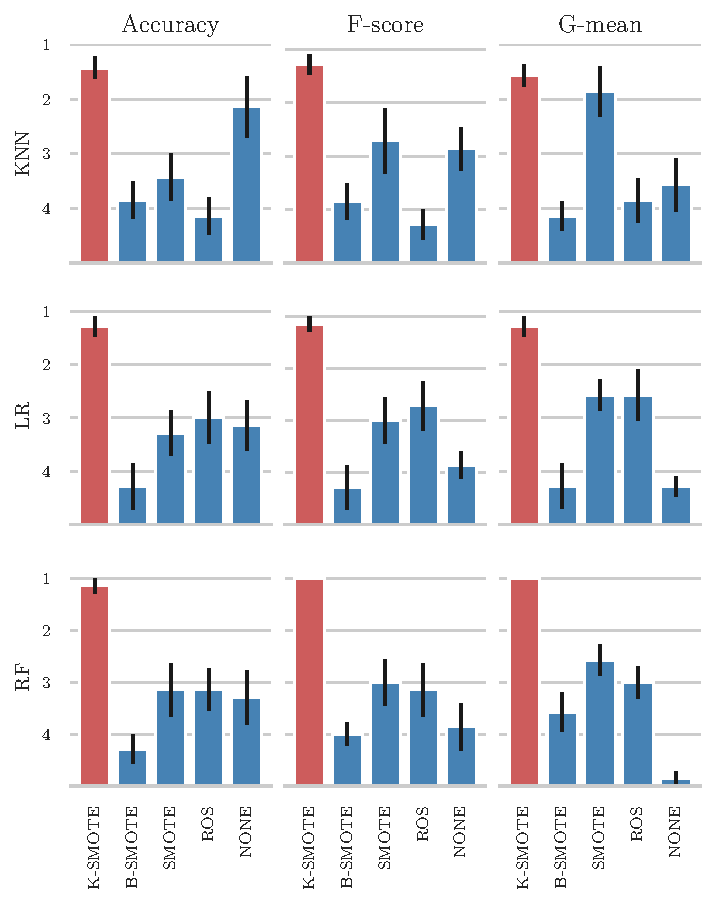
\includegraphics[width=.65\linewidth]{mean_rankings_bar_chart}
	\caption{%
    	Results for mean ranking of oversamplers across datasets.
    }~\label{fig:mean_sem_ranking}
\end{figure}

The mean cross-validation scores are shown in Table~\ref{tab:mean_sem_scores}.
As discussed previously in this section, the disparity of performance levels
across datasets makes the analysis of these scores less informative.

\begin{table}
	\centering
    \addtolength{\leftskip} {-2cm}
    \addtolength{\rightskip}{-2cm}
    \pgfplotstabletypeset[
        col sep=comma,
        string type,
        every head row/.style={%
            before row=\toprule,
            after row=\midrule
        },
        every last row/.style={after row=\bottomrule},
        string type,
    ]{figures/kmeans-smote-lulc/mean_sem_scores.csv}
    \caption{%
    	Mean cross-validation scores of oversamplers.
    }~\label{tab:mean_sem_scores}
\end{table}

The mean cross-validation scores for each dataset are presented in
Table~\ref{tab:cross_validation_scores} (see appendix). This table allows the direct
comparison of the performance metrics being analysed.

\subsection{Statistical Analysis}~\label{sec:statistical_analysis-kmeans}

The experiment's multi-dataset context was used to perform a Friedman
test~\cite{Friedman1937}. Table~\ref{tab:friedman_test_kmeans} shows the results
obtained in the Friedman test performed, where the null hypothesis is rejected
in all cases. The rejection of the null hypothesis implies that the
differences between the differences among the different oversamplers are not
random, in other words, these differences are statistically significant.

\begin{table}[ht]
    \centering
    \pgfplotstabletypeset[
        col sep=comma,
        string type,
        every head row/.style={%
            before row=\toprule,
            after row=\midrule
        },
        every last row/.style={after row=\bottomrule},
        string type,
    ]{figures/kmeans-smote-lulc/friedman_test.csv}
    \caption[Results for Friedman test.]{%
        Results for Friedman test. Statistical significance is tested at a
        level of $\alpha = 0.05$. The null hypothesis is that there is no
        difference in the classification outcome across oversamplers.
    }~\label{tab:friedman_test_kmeans}
\end{table}

A Wilcoxon signed-rank test \cite{Wilcoxon1945} was also performed to
understand whether K-means SMOTE's superiority was statistically significant
across datasets and oversamplers, as suggested in \cite{Demsar2006}. This
method is used as an alternative to the paired Student's t-test, since the
distribution of the differences between the two samples cannot be assumed as
normally distributed. The null hypothesis of the test is that K-means SMOTE's
performance is similar to the compared oversampler (i.e., the oversamplers
used follow a symmetric distribution around zero).

\begin{table}
    \centering
    \pgfplotstabletypeset[
        col sep=comma,
        string type,
        every head row/.style={%
            before row=\toprule,
            after row=\midrule
        },
        every last row/.style={after row=\bottomrule},
        string type,
    ]{figures/kmeans-smote-lulc/wilcoxon_test.csv}
    \caption[\textit{p-values} of the Wilcoxon signed-rank test.]{%
        \textit{p-values} of the Wilcoxon signed-rank test. Boldface values
        are statistically significant at a significance level of $\alpha =
        0.05$.
    }~\label{tab:wilcoxon_test_kmeans}
\end{table}

\subsection{Discussion}

The mean rankings presented in
Figure~\ref{fig:mean_sem_ranking} show that on average,
K-means SMOTE produced the best results for every classifier and performance
metric used. This is due to the clustering phase and subsequent selection of
data to be considered for oversampling. By successfully clustering and
selecting the relevant areas in the data space to oversample, the generation
of artificial instances is done only in the context of minority regions that
represent well their spectral signature.

As previously discussed, the direct comparison of performance metrics averaged
over various datasets is not recommended due to the varying levels of
performance of classifiers across datasets~\cite{Demsar2006}. Nonetheless,
these results are shown in Table~\ref{tab:mean_sem_scores} to provide a fuller
picture of the results obtained in the experiment. We found that on average
K-means SMOTE provides increased performance, regardless of the classifier and
performance metric used. More importantly, K-means SMOTE guaranteed a more
consistent performance across datasets and with less variability, which can be
attested in Figure~\ref{fig:mean_sem_ranking} and
Tables~\ref{tab:mean_sem_scores} and~\ref{tab:cross_validation_scores}.

As discussed in Subsection~\ref{sec:evaluation-metrics-kmeans}, Evaluation Metrics,
our results are consistent with the findings in~\cite{Olofsson2013,
Pontius2011}. Particularly, we consider the results obtained in our experiment
using Overall Accuracy to be less informative than the results obtained with
the remaining performance metrics, since this metric is affected by imbalanced
class distributions. The majority class bias in this metric can be observed in
our experiment in Figure~\ref{fig:mean_sem_ranking} with the
classifiers LR and KNN, where the control method (NONE) is only outperformed
by K-means SMOTE. This effect is observed with more detail in
Table~\ref{tab:mean_sem_scores}, where the benchmark oversamplers are
outperformed by the control method in 16 out of 63 tests (approximately 25\%).
Out of these, most refer to tests using overall accuracy among the four
datasets with highest IR, showing the overall accuracy's class imbalance bias
discussed in~\cite{Olofsson2013, Pontius2011}. The K-means SMOTE oversampler
is only outperformed by the control method in 3 of tests (all of them using
overall accuracy). This is an improvement over the benchmark oversamplers,
showing that generally K-means SMOTE is the best choice even when overall
accuracy is used as the main performance metric.

In the majority of the cases, K-means SMOTE was able to generate higher
quality data due to the non-random selection of data spaces to oversample.
This can be seen in the performance of the classifiers trained on top of this
data generation step, making it a more informed data generation method in the
context of LULC\@.

The performance of both oversamplers and classifiers is generally dependent on
the dataset being used. Although both absolute and relative scores between the
different oversamplers are dependent on the choice of metric and classifier,
K-means SMOTE's relative performance is consistent across datasets and
generally outperforms the remaining oversampling methods in 56 of the 63 tests
(approximately 89\%). The mean cross-validation results found in
Table~\ref{tab:cross_validation_scores} show that performance-wise, K-means
SMOTE is always better than or as good as SMOTE, with the exception of 4
situations (representing 6\% of the tests done), in which cases the percentage
point difference is neglectable ($\leq 0.1$ percentage points). 

The statistical tests showed that not only there is a statistically
significant difference across the oversamplers used in this problem (found in
the Friedman test presented in Table~\ref{tab:friedman_test_kmeans}), but also that
K-means SMOTE's superior performance is statistically significant at a level
of 0.05 in 27 out of 28 tests in the Wilcoxon signed-rank test shown in
Table~\ref{tab:wilcoxon_test_kmeans} (approximately 96\% of the tests performed).
This shows that, in most cases, the usage of k-Means SMOTE improves the
quality of LULC classification when compared to using SMOTE in its original
format, which remains the most popular oversampler among the remote sensing
community.

Although the usage of K-means SMOTE successfully captured the spectral
signatures of the minority classes, it was done using K-means, a
problem-agnostic clusterer. Consequently, the implementation of this method
using a GIS-specific clusterer that considers the geographical traits of
different regions (e.g., using the sampled pixels' geographical coordinates),
may be a promising direction towards the development of more appropriate
oversampling techniques in the remote sensing domain.

\section{Conclusion}~\label{sec:conclusion-kmeans} 

This research paper was motivated by the challenges faced when classifying
rare classes for LULC mapping. Cluster-based oversampling is especially useful
in this context because the spectral signature of a given class often varies,
depending on its geographical distribution and the time period within which
the image was acquired. This induces the representation of minority classes as
small clusters in the input space. As a result, training a classifier capable
of identifying LULC minority classes in the hyper/multi-spectral scene over
different areas or periods becomes particularly challenging. The clustering
procedure, performed before the data generation phase, allows for a more
accurate generation of minority samples, as it identifies these minority
clusters.

A number of existing methods to address the imbalanced learning problem were
identified and their limitations discussed. Typically, algorithm-based
approaches and cost-sensitive solutions are not only difficult to implement,
but they are also context dependent. In this paper we focused on oversampling
methods due to their widespread usage, easy implementation and flexibility.
Specifically, this paper demonstrated the efficacy of a recent oversampler,
K-Means SMOTE, applied in a multi-class context for Land Cover Classification
tasks. This was done with sampled data from seven well known and naturally
imbalanced benchmark datasets: Indian Pines, Pavia Center, Pavia University,
Salinas, Salinas A, Botswana and Kennedy Space Center. For each combination of
dataset, oversampler and classifier, the results of every classification task
was averaged across a 5 fold stratification strategy with 3 different
initialization seeds, resulting in a mean validation score of 15
classification tasks. The mean validation score of each combination was then
used to perform the analyses presented in this report.

In 56 out of 63 classification tasks (approximately 89\%), K-means SMOTE led
to better results than ROS, SMOTE, B-SMOTE and no oversampling. More
importantly, we found that K-Means SMOTE is always better or equal than the
second best oversampling method.  K-means SMOTE's performance was independent
from both the classifier and performance metric under analysis. In general,
K-means SMOTE shows a higher performance among the non tree-based classifiers
employed (LR and KNN) when compared with the remaining oversamplers, where
these oversamplers generally failed to improve the quality of classification.
Although these findings are case dependent, they are consistent with the
results presented in~\cite{Douzas2018}. The proposed method also had the most
consistent results across datasets, since it produced the lowest standard
deviations across datasets in 7 out of 9 cases for both analyses, either based
on ranking or mean cross-validation scores.

The proposed algorithm is a generalization of the original SMOTE algorithm. In
fact, the SMOTE algorithm represents a corner case of K-means SMOTE i.e., when
the number of clusters equals to 1. Its data selection phase differs from the
one used in SMOTE and Borderline SMOTE, providing artificially augmented
datasets with less noisy data than the commonly used methods. This allows the
training of classifiers with better defined decision boundaries, especially in
the most important regions of the data space (the ones populated by a higher
percentage of minority class instances).

As stated previously, the usage of this oversampler is technically simple. It
can be applied to any classification problem relying on an imbalanced dataset,
alongside any classifier. K-means SMOTE is available as an open source
implementation for the Python programming language (see
Subsection~\ref{sec:implementation-kmeans}).  Consequently, it can be a useful tool
for both remote sensing researchers and practitioners.

\thesischapter{%
    Increasing the Effectiveness of Active Learning: Introducing Artificial
    Data Generation in Active Learning for Land Use/Land Cover
    Classification
}{%
    Published as Joao Fonseca, Georgios Douzas, Fernando Bacao, in Remote
    Sensing, 2021
}~\label{chp:al-generator-lulc}


\graphicspath{{figures/al-generator-lulc/}}

\begin{adjustwidth}{30pt}{30pt}

    In remote sensing, Active Learning (AL) has become an important technique
    to collect informative ground truth data ``on-demand'' for supervised
    classification tasks. In spite of its effectiveness, it is still
    significantly reliant on user interaction, which makes it both expensive
    and time consuming to implement. Most of the current literature focuses on
    the optimization of AL by modifying the selection criteria and the
    classifiers used. Although improvements in these areas will result in more
    effective data collection, the use of artificial data sources to reduce
    human-computer interaction remains unexplored. In this paper, we introduce
    a new component to the typical AL framework, the data generator, a source
    of artificial data to reduce the amount of user-labeled data required in
    AL\@. The implementation of the proposed AL framework is done using
    Geometric SMOTE as data generator. We compare the new AL framework to the
    original one using similar acquisition functions and classifiers over
    three AL-specific performance metrics in seven benchmark datasets. We show
    that this modification of the AL framework significantly reduces cost and
    time requirements for a successful AL implementation in all of the
    datasets used in the experiment. 

\end{adjustwidth}

\vspace{.5cm}
\textbf{Keywords:} Active Learning; Artificial Data Generation; Land Use/Land Cover Classification;  Oversampling; SMOTE

\section{Introduction}~\label{sec:introduction-al-generator}

The technological development of air and spaceborne sensors, as well as the
increasing number of remote sensing missions have allowed the continuous
collection of large amounts of high quality remotely sensed data. This data is
often composed of multi and hyper spectral satellite imagery, essential for
numerous applications, such as Land Use/Land Cover (LULC) change detection,
ecosystem management~\cite{Nagai2020}, agricultural
management~\cite{Huang2018}, water resource management~\cite{Wang2018}, forest
management, and urban monitoring~\cite{Khatami2016}. Despite LULC maps being
essential for most of these applications, their production is still a
challenging task~\cite{Gavade2019, Wulder2018}. They can be updated using one
of the following strategies:

\begin{enumerate}
    \item Photo-interpretation. This approach consists of evaluating a patch's
        LULC class by a human operator based on orthophoto and satellite image
        interpretation~\cite{costa2020introducing}. This method guarantees a
        decent level of accuracy, as it is dependent on the interpreter's
        expertise and human error. Typically, it is an expensive,
        time-consuming task that requires the expertise of a
        photo-interpreter. This task is also frequently applied to obtain
        ground-truth labels for training and/or validating Machine Learning
        (ML) algorithms for related tasks~\cite{vermote2020remote,
        COSTANTINO2020}. 
    \item Automated mapping. This approach is based on the usage of a ML
        method or a combination of methods in order to obtain an updated LULC
        map. The development of a reliable automated method is still a
        challenge among the ML and remote sensing community, since the
        effectiveness of existing methods varies across applications and
        geographical areas~\cite{Gavade2019}. Typically, this method requires
        the existence of ground-truth data, which is frequently outdated or
        nonexistent for the required time frame~\cite{Nagai2020}. On the other
        hand, employing a ML method provides readily available and relatively
        inexpensive LULC maps. The increasing quality of state-of-the-art
        classification methods have motivated the application and adaptation
        of these methods in this domain~\cite{Maxwell2018}.
    \item Hybrid approaches. These approaches employ photo-interpreted data to
        augment the training dataset and improve the quality of automated
        mapping~\cite{Ruzicka2020}. It attempts to accelerate the
        photo-interpretation process by selecting a smaller sample of the
        study area to be interpreted. The goal is to minimize the inaccuracies
        found in the LULC map by supplying high-quality ground-truth data to
        the automated method. The final (photo-interpreted) dataset consists
        of only the most informative samples, \textit{i.e.}, patches that are
        typically difficult to classify for a traditional automated mapping
        method~\cite{Liu2020}. 
\end{enumerate}

The latter method is best know as AL\@. It is especially useful whenever there
is a shortage or even absence of ground-truth data and/or the mapping region
does not contain updated LULC maps~\cite{Su2020}. In a context of limited
sample-collection budget, the collection of the most informative samples
capable of optimally increasing the classification accuracy of a LULC map is
of particular interest~\cite{Su2020}. AL attempts to minimize the
human-computer interaction involved in photo-interpretation by selecting the
data points to include in the annotation process. These data points are
selected based on an uncertainty measure and represent the points close to the
decision borders. Afterwards, they are passed on for photo-interpretation and
added to the training dataset, while the points with the lowest uncertainty
values are ignored for photo-interpretation and classification. This process
is repeated until a convergence criterion is reached~\cite{Pasolli2016}. 

The relevant work developed within AL is described in detail in
Section~\ref{sec:al-sota-al-generator}. This paper attempts to address some of the
challenges found in AL, mainly inherited from automated and photo-interpreted
mapping: mapping inaccuracies and time consuming human-computer interactions.
These challenges have different sources:

\begin{enumerate}
    \item Human error. The involvement of photo-interpreters in the data
        labeling step carries an additional risk to the creation of LULC
        patches. The minimum mapping unit being considered, as well as the
        quality of the orthophotos and satellite images being used, are some of
        the factors that may lead to the overlooking of small-area LULC patches
        and label-noisy training data~\cite{Pelletier2017}.
    \item High-dimensional datasets. Although the amount of bands
        (\textit{i.e.}, features) present in multi and hyper spectral images
        contain useful information for automated classification, they also
        introduce an increased level of complexity and redundancy in the
        classification step~\cite{Stromann2020}. These datasets are often
        prone to the Hughes phenomenon, also known as the curse of
        dimensionality. 
    \item Class separability. Producing an LULC map considering classes with
        similar spectral signatures makes them difficult to
        separate~\cite{Alonso-Sarria2019}. A lower pixel resolution of the
        satellite images may also imply mixed-class pixels, which may lead to
        both lower class separability as well as higher risk of human error.
    \item Existence of rare land cover classes. The varying morphologies of
        different geographical regions naturally implies an uneven distribution
        of land cover classes~\cite{Feng2018}. This is particularly relevant in
        the context of AL since the data selection method is based on a given
        uncertainty measure over data points whose class label is unknown.
        Consequently, AL's iterative process of data selection may disregard
        wrongly classified land cover areas belonging to a minority class.
\end{enumerate}

Research developed in the field of AL typically focus on the reduction of
human error by minimizing the human interaction with the process through the
development of more efficient classifiers and selection criteria within the
generally accepted AL framework. Concurrently, the problem of rare land cover
classes is rarely addressed. This is a frequent problem in the ML community,
known as the Imbalanced Learning problem. This problem exists whenever there
is an uneven between-class distribution in the dataset~\cite{Chawla2004}.
Specifically, most classifiers are optimized and evaluted using accuracy-like
metrics, which are designed to work primarily with balanced datasets.
Consequently, these metrics tend to introduce a bias towards the majority
class by attributing an importance to each class proportional to its relative
frequency~\cite{Maxwell2018}. As an example, such a classifier could achieve
an overall accuracy of 99\% on a binary dataset where the minority class
represents 1\% of the overall dataset and still be useless. A number of
methods have been developed to deal with this problem.  They can be
categorized into three different types of
approaches~\cite{Fernandez2013,Kaur2019}.  Cost-sensitive solutions perform
changes to the cost matrix in the learning phase. Algorithmic level solutions
modify specific classifiers to reinforce learning on minority classes.
Resampling solutions modify the training data by removing majority samples
and/or generating artificial minority samples. The latter is independent from
the context and can be used alongside any classifier.  Since we are interested
in the introduction of artificial data generation in AL, we will analyze the
state-of-the-art on resampling techniques (specifically oversampling) in
Section~\ref{sec:ovs-sota-al-generator}.

In this paper, we propose a novel AL framework to address two limitations
commonly found in the literature: minimize human-computer interaction and
reduce the class imbalance bias. This is done with the introduction of an
additional component in the iterative AL procedure (the generator) that
is used to generate artificial data to both balance and augment the training
dataset. The introduction of this component is expected to reduce the number
of iterations required until the classifier reaches a satisfactory
performance.

This paper is organized as follows: Section~\ref{sec:introduction-al-generator} explains
the problem and its context, Sections~\ref{sec:al-sota-al-generator} and~\ref{sec:ovs-sota-al-generator}
describe the state of the art in AL and Oversampling techniques,
Section~\ref{sec:proposed-method-al-generator} explains the proposed method,
Section~\ref{sec:methodology-al-generator} covers the datasets, evaluation metrics, ML
classifiers and experimental procedure, Section~\ref{sec:results-al-generator} presents the
experiment's results and discussion and Section~\ref{sec:conclusion-al-generator} presents
the conclusions drawn from our findings.

\section{Active Learning Approaches}~\label{sec:al-sota-al-generator}

As the amount of unlabeled data increases, the interest and practical
usefulness of AL follows that trend~\cite{Kottke2017}. AL is used as the
general definition of frameworks aiming to train a learning system in multiple
steps, where a set of new data points are chosen and added to the training
dataset each time~\cite{Ruzicka2020}. Typically, an AL framework is composed
of the following elements~\cite{Sverchkov2017,Su2020,Ruzicka2020}:

\begin{enumerate}
    \item Unlabeled dataset. Consists of the original data source (or a sample
        thereof). It is used in combination with the chooser and the selection
        criterion to expand the training dataset in regions where the
        classification uncertainty is higher. Therefore, the unlabeled
        dataset is used for both producing the initial training
        dataset by selecting a set of instances for the
        supervisor to annotate (discussed in point 3) and calculating the
        uncertainty map to augment the training dataset.
    \item Supervisor. A human annotator (or team of human
        annotators) to which the uncertainty map is
        presented to. The supervisor is responsible for annotating unlabeled
        instances to be added to the augmented dataset. In remote sensing, the
        supervisor is typically a photo-interpreter, as is the case
        in~\cite{li2020}. Some of the research also refers to the supervisor
        as the \textit{oracle}~\cite{Ruzicka2020, Yoo2019, Aghdam2019,
        Cawley2011}.
    \item Initial training dataset. It is a small, labeled sample of
        the original data source used to initiate the first AL
        iteration. The size of the initial training sample normally varies
        between no instances at all and 10\% of the unlabeled
        dataset~\cite{Li2013}.
    \item Current and expanded training dataset. It is the concatenation of
        the initial training dataset and the datasets labeled by the
        supervisor in past iterations (discussed in point 2).
    \item Chooser (classifier). Produces the class probabilities for each
        unlabeled instance.
    \item Selection criterion. It quantifies the chooser's uncertainty level
        for each instance belonging to the unlabeled dataset. It is typically
        based on the class probabilities assigned by the chooser. In some
        situations, the chooser and the selection criterion are grouped
        together under the concept \textit{acquisition
        function}~\cite{Ruzicka2020} or \textit{query function}~\cite{Su2020}.
        Some of the literature refers to the selection criterion by using the
        concept \textit{sampling scheme}~\cite{Liu2020}.
\end{enumerate}

Figure~\ref{fig:al_typical} schematizes the steps involved in a complete AL
iteration. For a better context within the remote sensing domain, the
prediction output can be identified as the LULC map. This
framework starts by collecting unlabeled data from the original data source.
It is used to generate a random initial training sample and is labeled by the
supervisor. In practical applications, the supervisor is frequently a group of
photo-interpreters~\cite{Kottke2017}. The chooser is trained on the resulting
dataset and is used to predict the class probabilities on the unlabeled
dataset. The class probabilities are fed into a selection criterion to
estimate the prediction's uncertainty, out of which the instances with the
highest uncertainty will be selected. This calculation is motivated by the
absence of labels in the uncertainty dataset. Therefore, it is impossible to
estimate the prediction's accuracy in the unlabeled dataset in a real case
scenario. The iteration is completed when the selected points are tagged by
the supervisor and added to the training dataset (\textit{i.e.}, the augmented
dataset). 

\begin{figure}[htb]
	\centering
	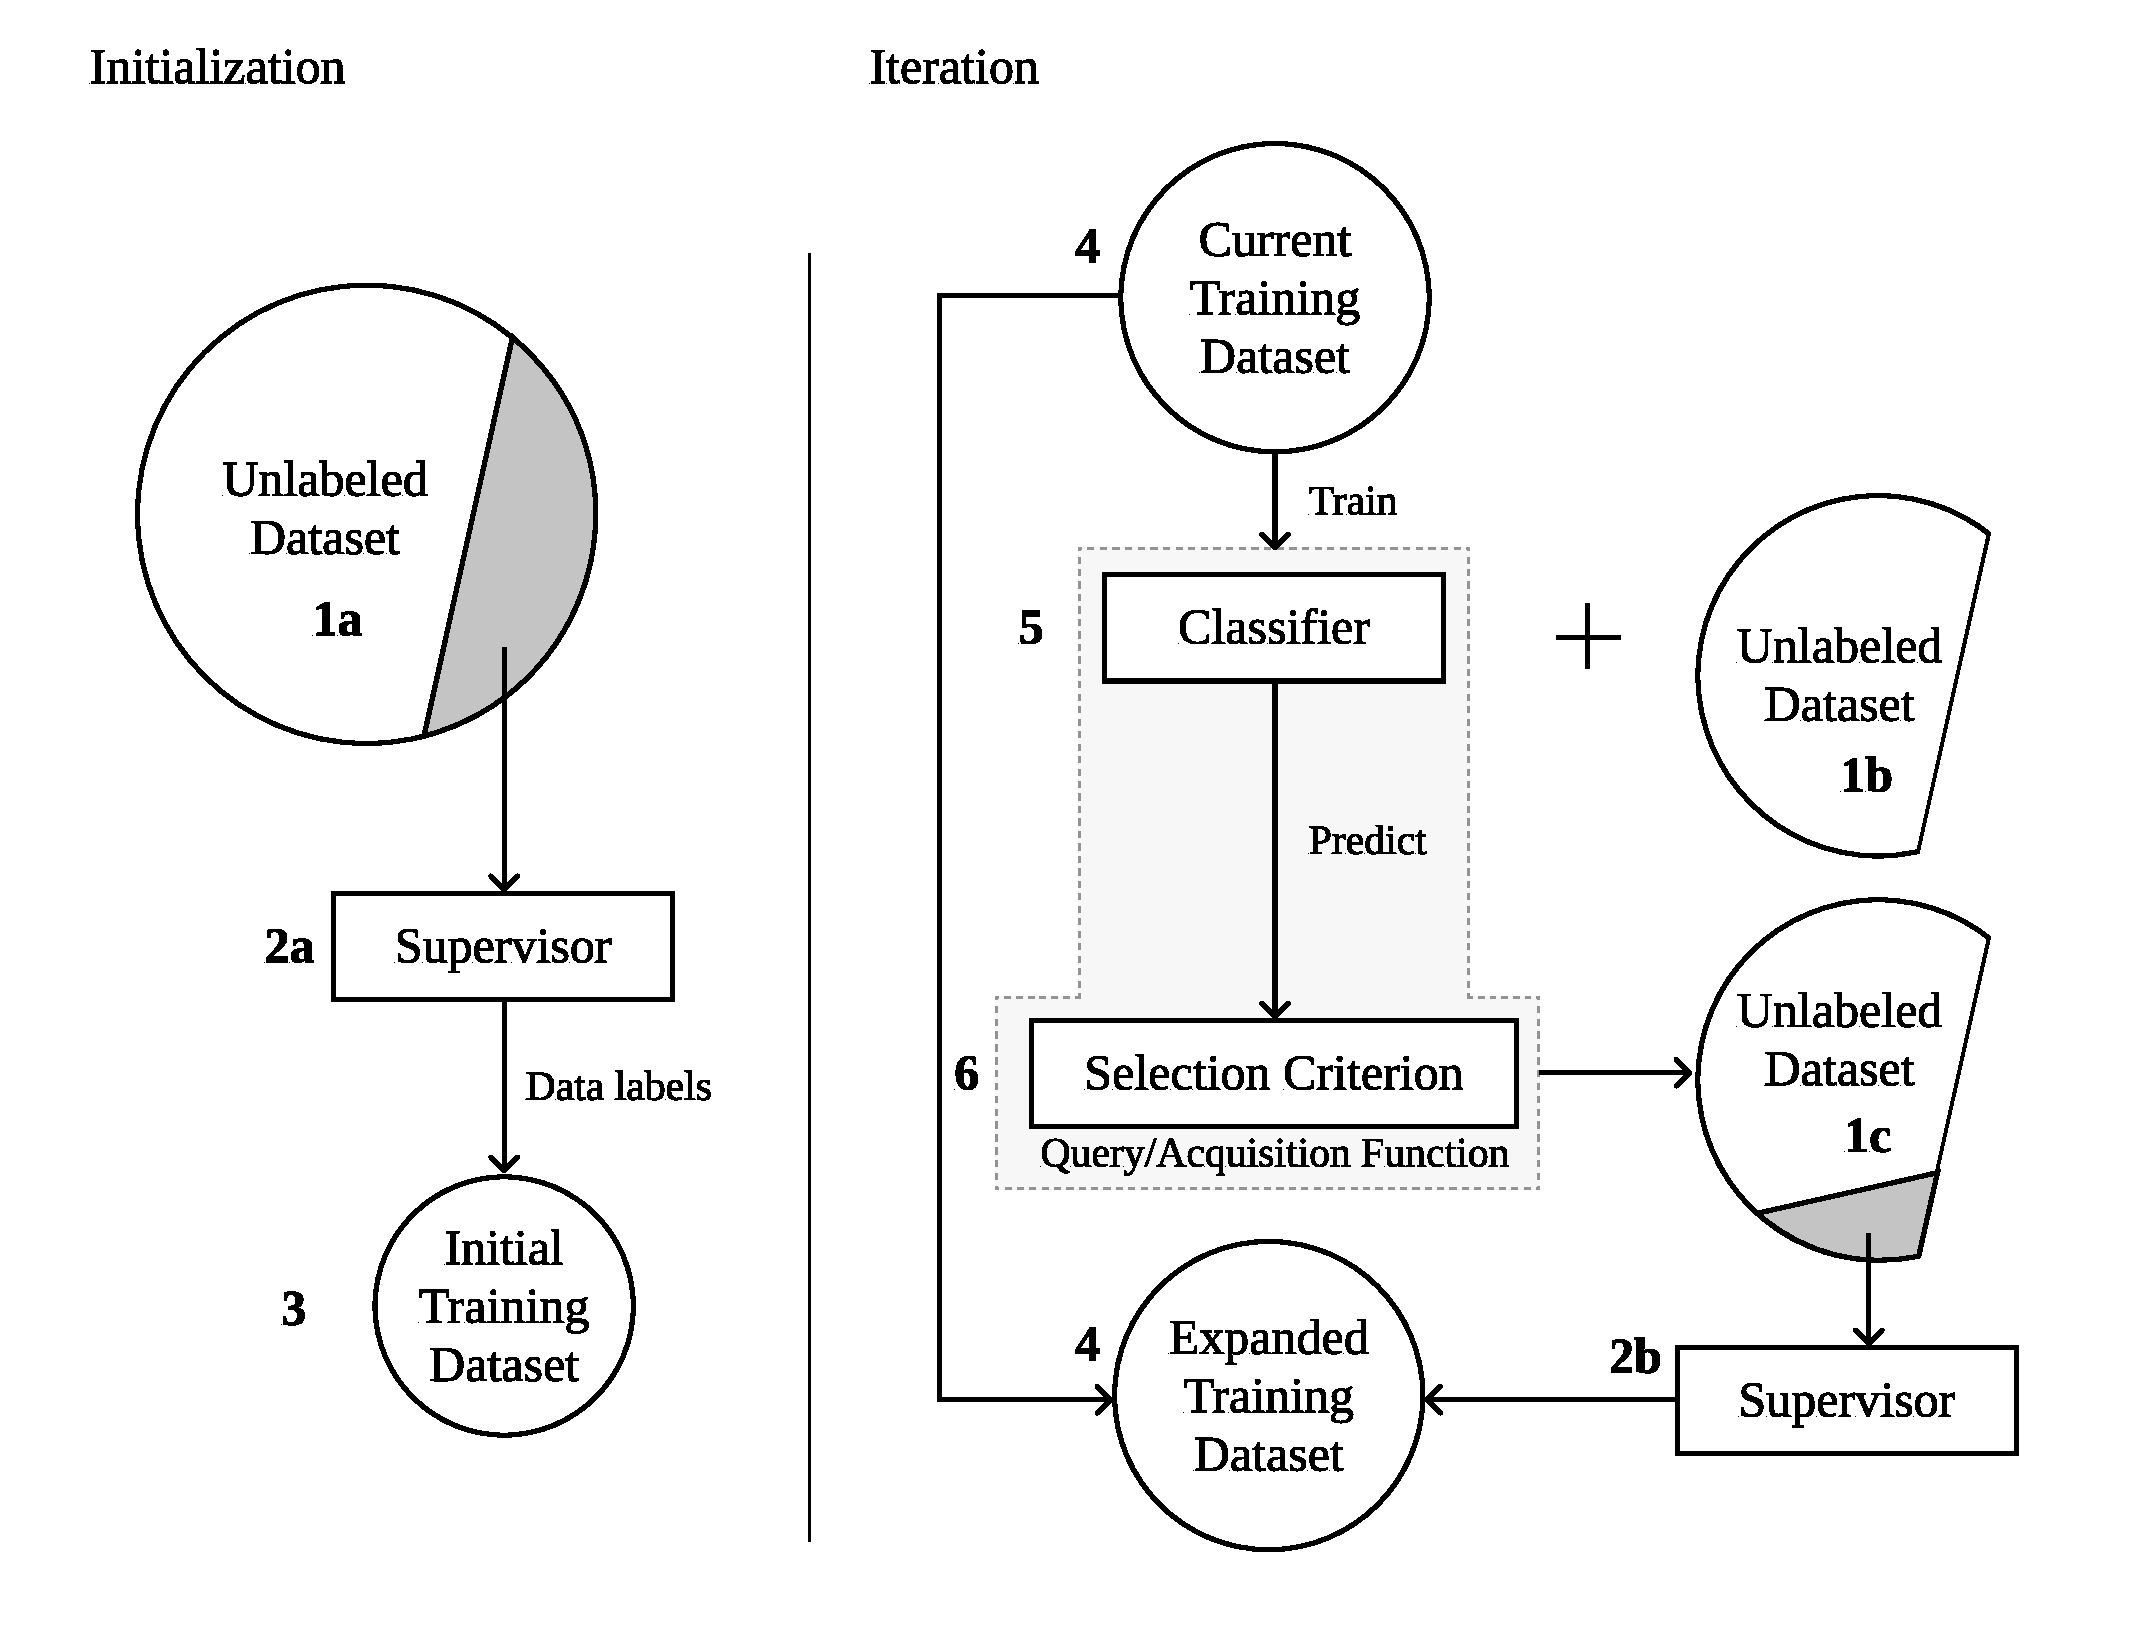
\includegraphics[width=.7\linewidth]{al_typical}
	\caption{Diagram depicting the typical AL framework.
    }~\label{fig:al_typical}
\end{figure}

A common challenge found in AL tasks is ensuring the consistency of AL over
different initializations~\cite{Kottke2017}. There are two factors involved in
this phenomenon. On one hand, the implementation of the same method over
different initializations may result in significantly different initial
training samples, amounts to varying accuracy curves. On the other hand, the
lack of a robust selection criterion and/or classifier may
also result in inconsistencies across AL experiments with different
initializations. This phenomenon was observed and documented in a LULC
classification context in~\cite{tuia2011using}.

The classification method plays a central role in the efficacy of AL. The
classifier used should be able to generalise with a relatively small training
dataset. Specifically, deep learning models are used in image classification
due to its capability of producing high quality predictions. Although, to make
such models generalizable the training set must be large enough, making its
suitability for AL applications an open challenge~\cite{Cao2020, Wu2020,
Bi2019}. Some studies in the Remote Sensing domain were developed to address
this gap. In~\cite{Cao2020, Bi2019}, the authors propose a deep learning-based
AL approach by training the same Convolutional Neural Network incrementally
across iterations and smoothen the decision boundaries of the model using the
Markov Random Field model and a Best-versus-Second Best labelling approach.
This allows the introduction of additional data variability in the final
training dataset. Another study~\cite{Wu2020} combined transfer learning,
active classification and segmentation techniques for vehicle detection. By
combining different techniques, they were able to produce a classification
mechanism that performed well when the amount of training data is limited.
However, the exploration of advanced deep learning classifiers in AL is
still limited. In~\cite{Hu2020}, the authors show that deep learning
classifiers performs well on LULC classification, but are still not
generalizable for different geographical regions or periods. Specifically, AL
methods are still incapable of providing generalizable deep learning
classifiers, which benefit from multiple advantages. The development of
Convolutional Neural Networks with both 2 and 3-dimensional convolutions was
explored in~\cite{Roy2019} and reported superior classification performance on
benchmark datasets. However, a large amount of training data was used to
produce the final classification map.

Selecting an efficient selection criterion is particularly important to find
the instances closest to the decision border (\textit{i.e.}, instances
difficult to classify)~\cite{Shrivastava2021}. Therefore, many AL related
studies focus on the design of the query/acquisition function~\cite{Su2020}.

\subsection{Non-informed selection criteria}

Only one non-informed (\textit{i.e.}, random) selection criterion was found in
the literature. Random sampling selects unlabeled instances without
considering any external information produced by the chooser. Since the method
for selecting the unlabeled instances is random, this method disregards the
usage of a chooser and is comparatively worse than any other selection
criterion. However, random sampling is still a powerful baseline
method~\cite{Cawley2011}. 

\subsection{Ensemble-based selection criteria}

Ensemble disagreement is based on the class predictions of a set of
classifiers. The disagreement between all the predictions for a given
instance is a common measure for uncertainty, although computationally
inefficient~\cite{Ruzicka2020,Pasolli2016}. It is calculated using the set of
classifications over a single instance, given by the number of votes
assigned to the most frequent class~\cite{Shrivastava2021}. This method was
implemented successfully for complex applications such as deep active
learning~\cite{Ruzicka2020}.

Multiview~\cite{Muslea2006} consists on the training of multiple independent
classifiers using different views, which correspond to the selection of subsets
of features or instances in the dataset. Therefore, it can be seen as a
bootstrap aggregation (bagging) ensemble disagreement method. It is represented
by the maximum disagreement score out of set of disagreements calculated for
each view~\cite{Shrivastava2021}. A lower value for this metric means a higher
classification uncertainty. Multiview-based maximum disagreement has been
successfully applied to hyper-spectral image classification in~\cite{Di2012}
and~\cite{Zhou2014}.

An adapted disagreement criterion for an ensemble of $k$-nearest neighbors has
been proposed in~\cite{Pasolli2016}. This method employs a $k$-nearest
neighbors classifier and computes an instance's classification uncertainty
based on the neighbors' class frequency using the maximum disagreement metric
over varying values for $k$. As a result, this method is comparable to
computing the dominant class' score over a weighted $k$-nearest neighbors
classifier. This method was also used on a multimetric active learning
framework~\cite{Zhang2016}.

Another relevant ensemble-based selection criterion is the binary random
forest-based query model~\cite{Su2020}. This method employs a one-versus-one
ensemble method to demonstrate an efficient data selection method using the
estimated probability of each binary random forest and determining the
classification uncertainty based on the probabilities closest to 0.5
(\textit{i.e.}, the least separable pair of classes are used to determine the
uncertainty value). However, this study fails to compare the proposed method
with other benchmark methods, such as random sampling.

\subsection{Entropy-based criteria}

A number of contributions have focused on entropy-based querying. The
application of entropy is common among active deep learning
applications~\cite{Aghdam2019}, where the training of an ensemble of
classifiers is often too expensive. 

Entropy query-by-bagging (EQB), also defined as maximum
entropy~\cite{Liu2020}, is an ensemble approach of the entropy selection
criterion, originally proposed in~\cite{Tuia2009}. This strategy uses the set
of predictions produced by the ensemble classifier to calculate those many
entropy measurements. The estimated uncertainty measure for one instance is
given by the maximum entropy within that set. EQB was observed to be an
efficient selection criterion. Specifically,~\cite{Shrivastava2021} applied
EQB on hyper-spectral remote sensing imagery using Support Vector Machines
(SVM) and Extreme Learning Machines (ELM) as choosers, achieving optimal
results when combining EQB with ELM\@. Another study successfully implemented
this method on an active deep learning application~\cite{Liu2020}. Another
study improved over this method with a normalized EQB selection
criterion~\cite{Copa2010}.

\subsection{Other relevant criteria}

Margin Sampling is a SVM-specific criterion, based on the distance of a given
point to the SVM's decision boundary~\cite{Shrivastava2021}. This method is
less popular than the remaining methods because it is limited to one type of
chooser (SVMs). One extension of this method is the multiclass level
uncertainty~\cite{Shrivastava2021}, calculated by subtracting the instance's
distance to the decision boundaries of the two most probable
classes~\cite{Demir2011}.

The Mutual Information-based (MI) criterion selects the new training instances
by maximizing the mutual information between the classifier and class labels
in order to select instances from regions that are difficult to classify.
Although this method is commonly used, it is frequently outperformed by the
breaking ties selection criterion~\cite{Li2011,Liu2018}.

The breaking ties (BT) selection criterion was originally introduced
in~\cite{Luo2003}. It consists of the subtraction between the probabilities of
the two most likely classes. Another related method is Modified Breaking Ties
scheme (MBT), which aims at finding the instances containing the largest
probabilities for the dominant class~\cite{Liu2018,Li2013a}

Another type of selection criteria identified is the loss prediction
method~\cite{Yoo2019}. This method replaces the selection criterion with a
predictor whose goal is to estimate the chooser's loss for a given
prediction. This allows the new classifier to estimate the prediction loss on
unlabeled instances and select the ones with the highest predicted loss.

Some of the literature fails to specify the strategy employed, although
inferring it is generally intuitive. For example,~\cite{Ertekin2007}
successfully used AL to address the imbalanced learning problem. They employed
an ensemble of SVMs as the chooser, as well as an ensemble-based selection
criterion. All of the research found related to this topic focused on the
improvement of AL through modifications on the selection criterion and
classifiers used. None of these publications proposed significant variations
to the original AL framework.

\section{Artificial Data Generation Approaches}~\label{sec:ovs-sota-al-generator}

The generation of artificial data is a common approach to address imbalanced
learning tasks~\cite{Kaur2019}, as well as improving the effectiveness of
supervised learning tasks~\cite{DeVries2017}. In recent years some
sophisticated data generation approaches were developed. However, the scope of
this work is to propose the integration of a generator within the AL
framework. To do this, we will focus on heuristic data generation approaches,
specifically, oversamplers.

Heuristic data resampling methods employ local and/or global information to
generate new, relevant, non-duplicate instances. These methods are most
commonly used to populate minority classes and balance the between-class
distribution of a dataset. The Synthetic Minority Oversampling Technique
(SMOTE)~\cite{Chawla2002} is a popular heuristic oversampling algorithm,
proposed in 2002. The simplicity and effectiveness of this method contributes
to its prevailing popularity. It generates a new instance through a linear
interpolation of a randomly selected minority-class instance and one of its
randomly selected $k$-nearest neighbors. The implementation of SMOTE for LULC
classification tasks has been found to improve the quality of the predictors
used~\cite{Jozdani2019,Bogner2018}. Despite its popularity, its drawbacks
motivated the development of other oversampling methods~\cite{Douzas2019}.

Geometric SMOTE (G-SMOTE)~\cite{Douzas2019} introduces a modification of the
SMOTE algorithm in the data generation mechanism to produce artificial
instances with higher variability. Instead of generating artificial data as a
linear combination of the parent instances, it is done within a deformed,
truncated hyper-spheroid. G-SMOTE generates an artificial instance
$\overrightarrow{z}$ within a hyper-spheroid, formed by selecting a minority
instance $\overrightarrow{x}$ and one of its nearest neighbors
$\overrightarrow{y}$, as shown in Figure~\ref{fig:data_generation}. The
truncation and deformation parameters define the shape of the spheroid's
geometry. The method also modifies the selection strategy for the $k$-nearest
neighbors, accepting the generation of artificial instances using instances
from different classes, as shown in Figure~\ref{fig:data_generation}d. The
modification of both selection and generation mechanisms addresses the main
drawbacks found in SMOTE, the generation of both noisy data (\textit{i.e.,}
generate minority class instances within majority class regions) and
near-duplicate minority class instances~\cite{Douzas2019}. G-SMOTE has shown
superior performance when compared with other oversampling methods for LULC
classification tasks, regardless of the classifier sed~\cite{Douzas2019rs}.

\begin{figure}
	\centering
	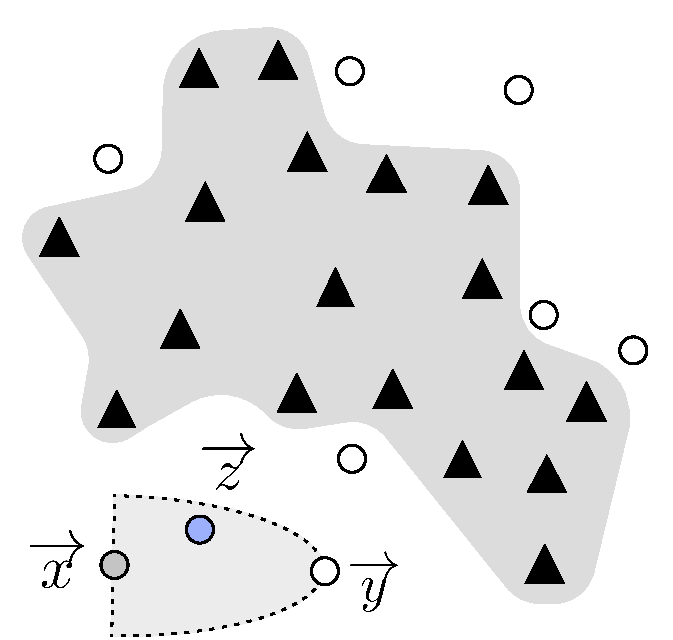
\includegraphics[width=.35\linewidth]{data_generation}
    \caption[Example of G-SMOTE's generation process.]{Example of G-SMOTE's
        generation process. G-SMOTE randomly selects instance
        $\protect\overrightarrow{x}$ and one of its nearest neighbors
        $\protect\overrightarrow{y}$ to produce instance
        $\protect\overrightarrow{z}$.
    }~\label{fig:data_generation}
\end{figure}

\section{Proposed method}~\label{sec:proposed-method-al-generator}

Within the literature identified, most of the work developed in the AL domain
revolved around improving the quality of classification algorithms and/or
selection criteria. Although these methods allow earlier convergence of the
AL iterative process, the impact of these methods are only observed between
iterations. Consequently, none of these contributions focused on the
definition of decision borders within iterations. The method proposed in this
paper modifies the AL framework by introducing an artificial data generation
step within AL's iterative process. We define this component as the generator
and is intended to be integrated into the AL framework as shown in
Figure~\ref{fig:al_new}. 

This modification, by using a new source of data to augment the training set,
leverages the data annotation work conducted by the human operator. The
artificial data that is generated between iterations reduces the amount of
labeled data required to reach optimal performance and lower the amount of
human labor required to train a classifier to its optimal performance. This
process lowers the annotation and overall training costs by translating some
of the annotation cost into computational cost.

\begin{figure}
	\centering
	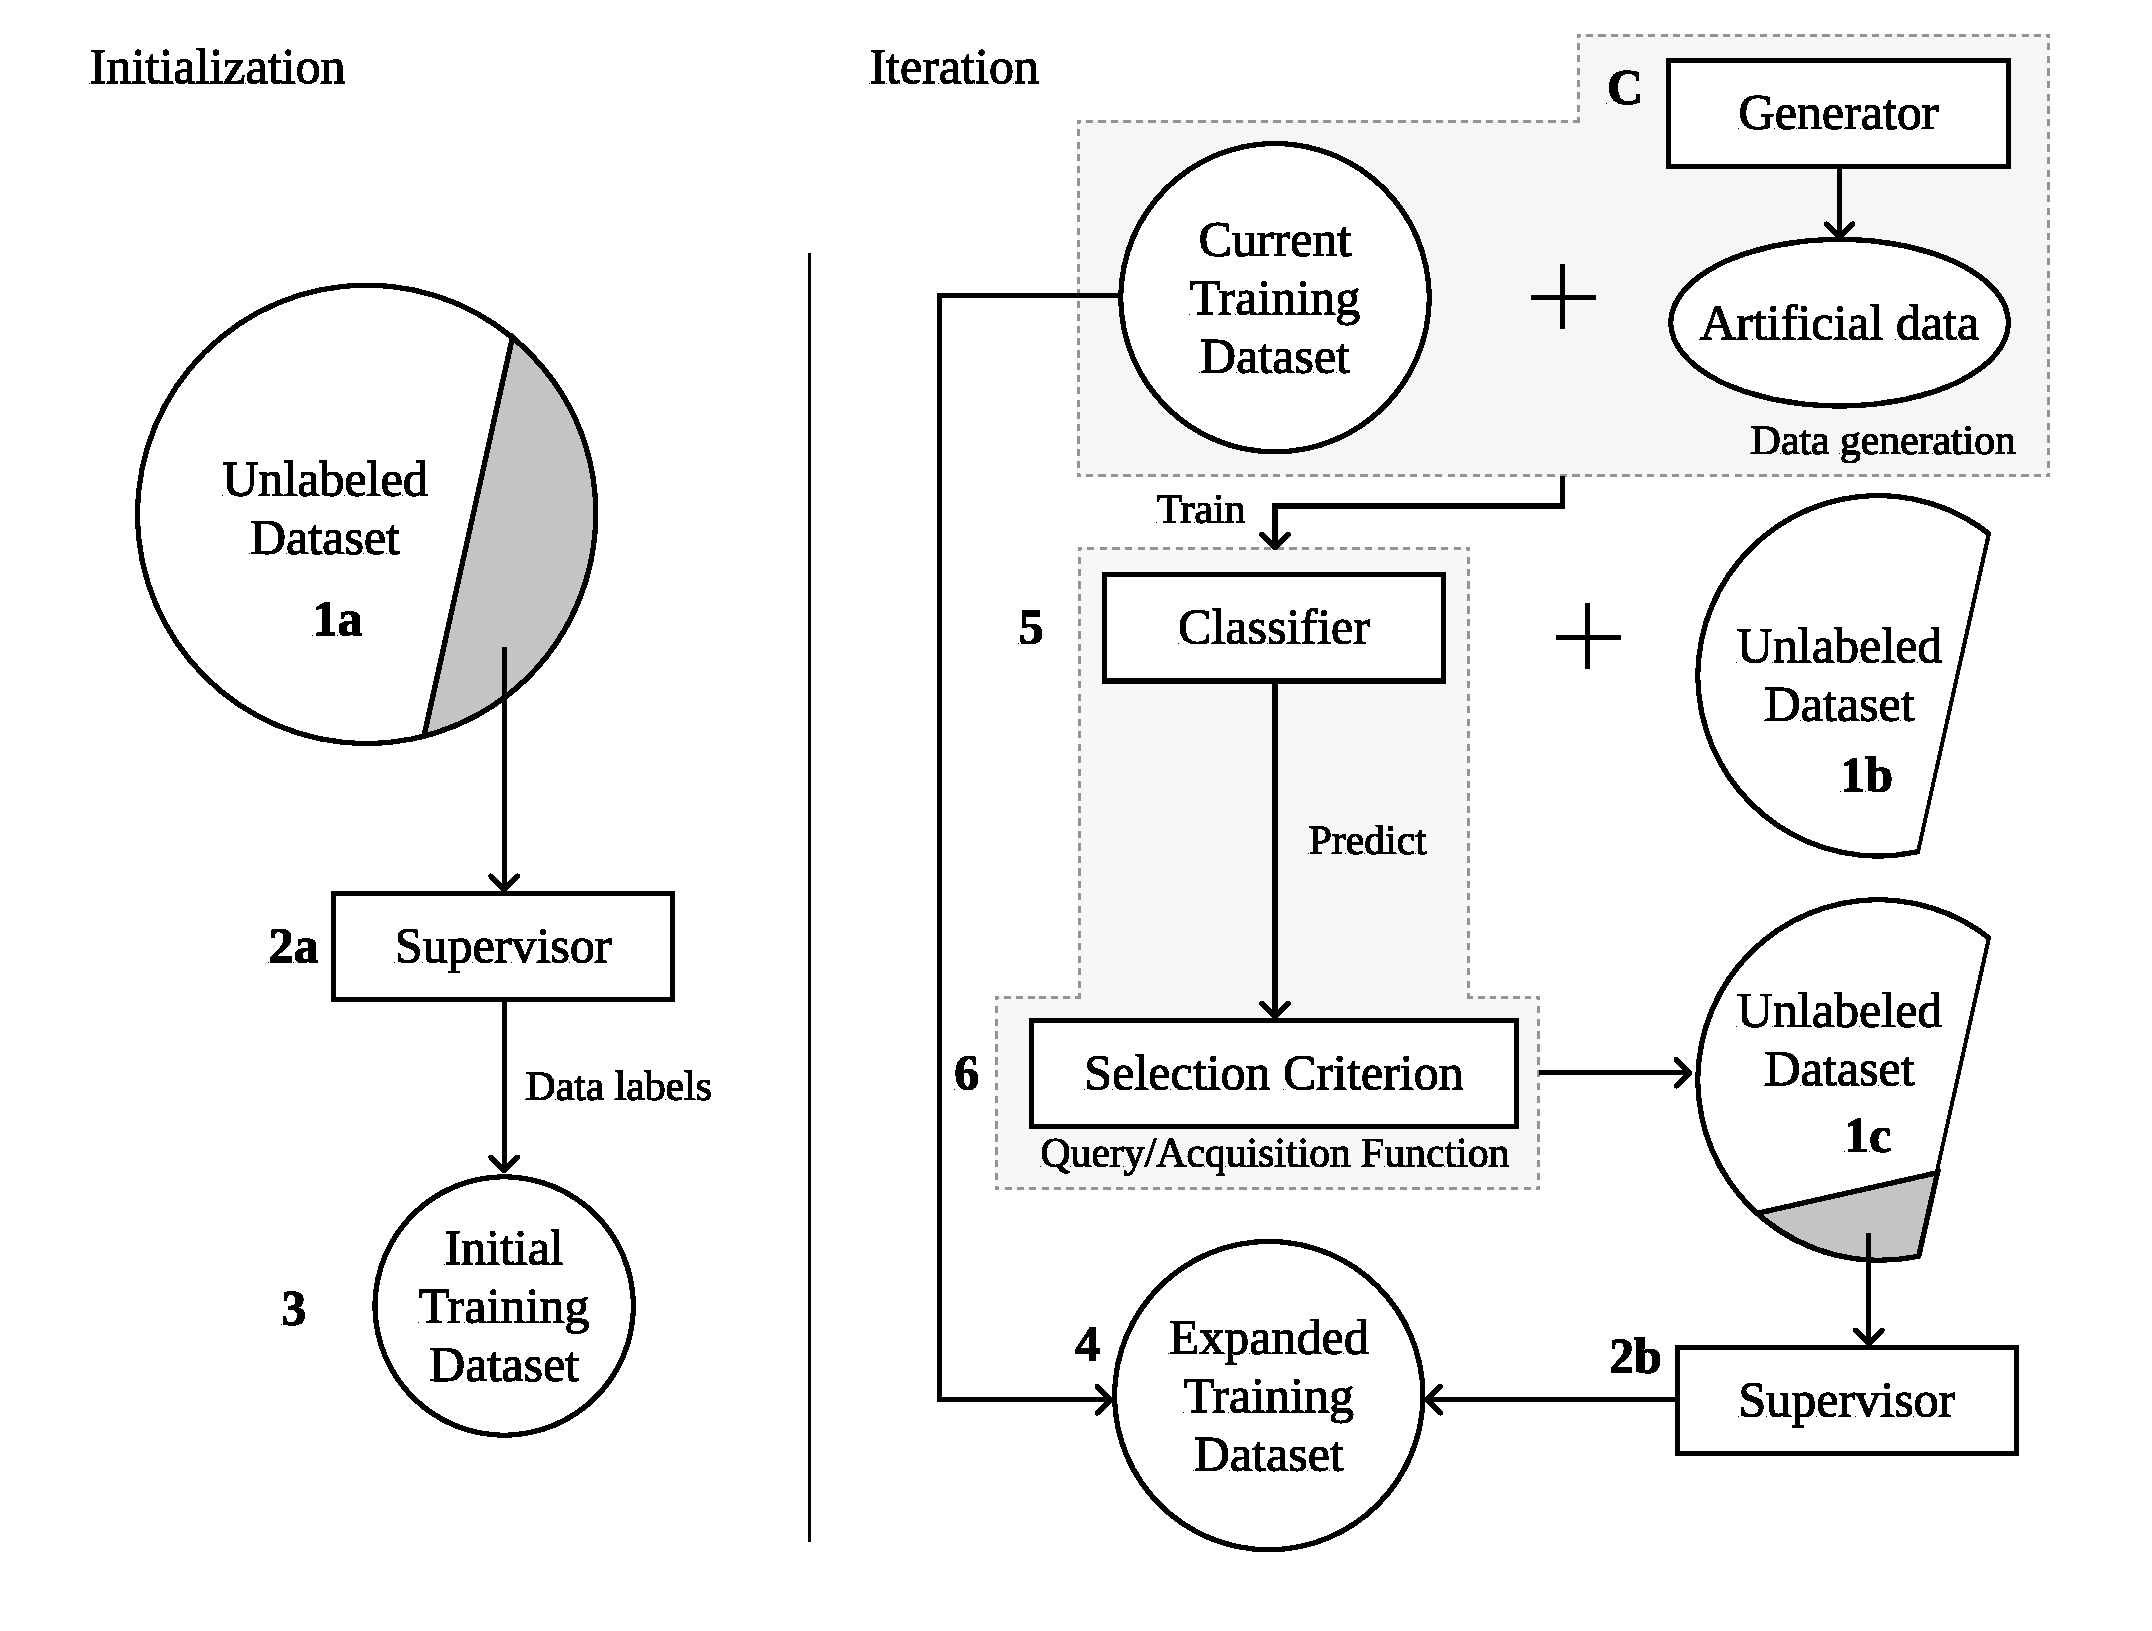
\includegraphics[width=.7\linewidth]{al_new}
    \caption[Proposed AL framework.]{%
        Proposed AL framework. This paper's contribution comprises a change in
        the AL framework through the introduction of a data generation
        mechanism, represented as the generator (marked with~\textit{C}),
        which is used to add artificial instances to the training dataset.
    }~\label{fig:al_new}
\end{figure}

This method leverages the capability of artificial data to introduce more data
variability into the augmented dataset and facilitate the chooser's training
phase with a more consistent definition of the decision boundaries at each
iteration. Therefore, any algorithm capable of producing artificial data, be
it agnostic or specific to the domain, can be employed. The artificial data is
only used to train the classifiers involved in the process and is discarded
once the training phase is completed. The remaining steps in the AL framework
remain unchanged. This method addresses the limitations found in the previous
sections:

\begin{enumerate}
    \item The convergence of classification performance should be anticipated
        with the clearer definition of the decision boundaries across
        iterations.
    \item Annotation cost is expected to reduce as the need for labeled
        instances reduces along with the early convergence of the
        classification performance.
    \item The class imbalance bias observed in typical classification tasks, as
        well as in AL is mitigated by balancing the class frequencies at each
        iteration.
\end{enumerate}

Although the performance of this method is shown within a LULC classification
context, the proposed framework is independent from the domain. The high
dimensionality of remotely sensed imagery make its classification particularly
challenging when the availability of labeled data is scarce and/or comes at a
high cost, being subjected to the curse of dimensionality. Consequently, it is
a relevant and appropriate domain to test this method.


\section{Methodology}~\label{sec:methodology-al-generator}

In this section we describe the datasets, evaluation metrics, oversampler,
classifiers, software used and the procedure developed. We demonstrate the
proposed method's efficiency over 7 datasets, sampled from publicly available,
well-known remote sensing hyperspectral scenes frequently found in remote
sensing literature. The datasets and sampling strategy are described in
Subsection~\ref{sec:datasets-al-generator}. On each of these datasets, we apply 3 different
classifiers over the entire training set to estimate the optimal
classification performance, the original AL framework as the baseline
reference and the proposed method using G-SMOTE as a generator, described in
Subsection~\ref{sec:machine_learning_algorithms-al-generator}. The metrics used to estimate
the performance of these algorithms are described in
Subsection~\ref{sec:evaluation_metrics-al-generator}. Finally, the experimental procedure
is described in Subsection~\ref{sec:experimental_procedure-al-generator}. 

Our methodology focuses on two objectives: (1) Comparison of optimal
classification performance among active learners and traditional supervised
learning and (2) Comparison of classification convergence efficiency among AL
frameworks.

\subsection{Datasets}~\label{sec:datasets-al-generator}

The datasets used were extracted from publicly available repositories
containing hyperspectral images and ground truth data. Additionally, all
datasets were collected using the same sampling procedure. The description of
the hyperspectral scenes used in this study is provided in
Table~\ref{tab:rs_scene_description}. These scenes were chosen because of
their popularity in the research community and their high baseline
classification scores. Consequently, demonstrating an outperforming method in
this context is particularly challenging and valuable.

\begin{table}
	\centering
    \addtolength{\leftskip} {-2cm}
    \addtolength{\rightskip}{-2cm}
    \pgfplotstabletypeset[
        col sep=semicolon,
        string type,
        every head row/.style={%
            before row=\toprule,
            after row=\midrule
        },
        every last row/.style={after row=\bottomrule},
        string type,
    ]{figures/al-generator-lulc/rs_scene_description.csv}
    \caption[Description of the hyperspectral scenes used in this experiment.]{%
        Description of the hyperspectral scenes used in this experiment. The
        column ``Res. (m)'' refers to the resolution of the sensors (in
        meters) that captured each of the scenes.
    }~\label{tab:rs_scene_description}
\end{table}

The Indian Pines scene~\cite{Baumgardner2015} is composed of agriculture fields
in approximately two thirds of its coverage, low density buildup areas and
natural perennial vegetation in the remainder of its area (see
Figure~\ref{fig:scenes}a). The Pavia Centre and University scenes are
hyperspectral, high-resolution images containing ground truth data composed of
urban-related coverage (see Figures~\ref{fig:scenes}b
and~\ref{fig:scenes}c). The Salinas and Salinas A scenes contain
at-sensor radiance data. As subset of Salinas, the Salinas A scene contains
contains the vegetables fields present in Salinas and the latter is also
composed of bare soils and vineyard fields (see Figures~\ref{fig:scenes}d
and~\ref{fig:scenes}e). The Botswana scene contains ground truth data
composed of seasonal swamps, occasional swamps, and drier woodlands located in
the distal portion of the Delta (see Figure~\ref{fig:scenes}f). The Kennedy
Space Center scene contains a ground truth composed of both vegetation and
urban-related coverage (see Figure~\ref{fig:scenes}g).

\begin{figure}
	\centering
	\includegraphics[width=.85\linewidth]{scenes}
    \caption[Gray scale visualization of a band and ground truth of each scene
        used in this study.]{%
        Gray scale visualization of a band (top row) and ground truth (bottom
        row) of each scene used in this study. (a) Indian Pines, (b) Pavia
        Centre, (c) Pavia University, (d) Salinas, (e) Salinas A, (f)
        Botswana, (g) Kennedy Space Center 
    }~\label{fig:scenes}
\end{figure}

The sampling strategy is similar to all datasets. The pixels without a ground
truth label are first discarded. All the classes with cardinality lower than
150 are also discarded. This is done to maintain feasible Imbalance Ratios (IR)
across datasets (where $IR = \frac{count(C_{maj})}{count(C_{min})}$). Finally,
a stratified sample of 1500 instances are selected for the experiment. The
resulting datasets are described in
Table~\ref{tab:datasets_description_al_generator}. The
motivation for this strategy is three fold: (1) reduce the datasets to a
manageable size and allow the experimental procedure to be completed within a
feasible time frame, (2) ensure the relative class frequencies in the scenes
are preserved and (3) ensure equivalent analyses across datasets and AL
frameworks. In this context, a fixed number of instances per dataset is
especially important to standardize the AL-related performance metrics.

\begin{table}
    \centering
    \addtolength{\leftskip} {-2cm}
    \addtolength{\rightskip}{-2cm}
    \pgfplotstabletypeset[
        col sep=comma,
        string type,
        every head row/.style={%
            before row=\toprule,
            after row=\midrule
        },
        every last row/.style={after row=\bottomrule},
    ]{figures/al-generator-lulc/datasets_description.csv}
    \caption[Description of the datasets collected from each corresponding
        scene.]{%
        Description of the datasets collected from each corresponding scene.
        The sampling strategy is similar to all scenes.
    }~\label{tab:datasets_description_al_generator}
\end{table}

\subsection{Machine Learning Algorithms}~\label{sec:machine_learning_algorithms-al-generator}

We use two different types of ML algorithms. A data generation algorithm, used
to form the generator, and classification algorithms, used to calculate the
classification uncertainties in the unlabeled dataset and predict the class
labels in the validation and test sets.

Although any method capable of generating artificial data can be used as a
generator, the one used in this experiment is an oversampler, originally
developed to deal with imbalanced learning problems. Specifically, we chose
G-SMOTE, a state-of-the-art oversampler.

Three classification algorithms are used. We use different types of
classifiers to test the framework's performance under varying situations:
neighbors-based, linear and ensemble models. The neighbors-based classifier
chosen was $K$-nearest neighbors (KNN)~\cite{Cover1967}, a logistic regression
(LR)~\cite{Nelder1972} is used as the linear model and a random forest
classifier (RFC)~\cite{Ho1995} was used as the ensemble model.

The acquisition function is completed by testing three different selection
criteria. Random selection is used as a baseline selection criterion, whereas
entropy and breaking ties are used due to their popularity and independence of
the classifier used.

\subsection{Evaluation Metrics}~\label{sec:evaluation_metrics-al-generator}

Since the datasets used in this experiment have an imbalanced distribution of
class frequencies, metrics such as the \textit{Overall Accuracy} (OA) and
\textit{Kappa coefficient} are insufficient to accurately depict
classification performance~\cite{Olofsson2013, Pontius2011}. Instead, metrics
such as Producer's Accuracy (or \textit{Recall}) and User's Accuracy (or
\textit{Precision}) can be used. Since they consist of ratios based on
True/False Positives (TP and FP) and Negatives (TN and FN), they provide per
class information regarding the classifier's classification performance.
However, in this experiment, the meaning and number of classes available in
each dataset varies, making these metrics difficult to synthesize.

The performance metric \textit{Geometric mean} (G-mean) and
\textit{F-score} are less sensitive to the data imbalance
bias~\cite{Jeni2013, Kubat1997}.  Therefore, we employ both of these
scorers. G-mean consists of the geometric mean of $Specificity = \frac{TN}{TN
+ FP}$ and $Sensitivity = \frac{TP}{TP+FN}$ (also known as
\textit{Recall})~\cite{Kubat1997}. Both metrics are calculated in a multiclass
context considering a one-versus-all approach. For multiclass problems, the
\textit{G-mean} scorer is calculated as its average per class values: 
        
\begin{equation*}
    \textit{G-mean} = \sqrt{\overline{Sensitivity}_i \times
    \overline{Specificity}_i}
\end{equation*}

The F-score performance metric is the harmonic mean of \textit{Precision} and
\textit{Recall}. The two metrics are also calculated considering a
one-versus-all approach. The \textit{F-score} for the multi-class case can be
calculated using its average per class values~\cite{He2009}:

\begin{equation*}
    \textit{F-score}=2\frac{\overline{Precision} \times
    \overline{Recall}}{\overline{Precision} + \overline{Recall}}
\end{equation*}
 
The comparison of classification convergence across AL frameworks and
selection criteria is done using 2 AL-specific performance metrics.
Particularly, we follow the recommendations found in~\cite{Kottke2017}. Each
AL configuration is evaluated using the \textit{Area Under the Learning Curve}
(AULC) performance metric. It is the sum of the classification performance
values of all iterations. To facilitate the analysis of the results, we fix
the range of this metric between $[0,1]$ by dividing it with the total amount
of iterations (\textit{i.e.}, the maximum performance area). 

The \textit{Data Utilization Rate} (DUR)~\cite{Reitmaier2013} metric consists
of the ratio between the number of instances required to reach a given G-mean
score threshold by an AL strategy and an equivalent baseline strategy. For
easier interpretability, we simplify this metric by using the percentage
of training data used by an AL strategy to reach the performance threshold,
instead of presenting these values as a ratio of the baseline strategy. The
DUR metric is measured at 9 different performance levels, between
0.6 and 0.95 G-mean scores at a 0.05 step.

\subsection{Experimental Procedure}~\label{sec:experimental_procedure-al-generator}

A common practice in methodological evaluations is the implementation of an
offline experiment~\cite{Kagy2019}. It consists of using an existing set of
labeled data as a proxy for the population of unlabeled instances. Because the
dataset is already fully labeled, the supervisor's typical annotation process
involved in each iteration is done at zero cost. Each AL and classifier
configuration is tested using a stratified 5-fold cross validation testing
scheme. For each round, the larger partition is split in a stratified fashion
to form a training and validation set (containing 20\% of the original
partition). The validation set is used to evaluate the convergence efficiency
of active learners; the chooser's classification performance metrics and
amount of data points used at each iteration are used to compute the AULC and
DUR\@. Additionally, within the AL iterative process, the classifier with
optimal performance on the validation set is evaluated using the test set. In
order to further reduce possible initialization biases, this procedure is
repeated 3 times with different initialization seeds and the results of all
runs are averaged (\textit{i.e.}, each configuration is trained and evaluated
15 times). Finally, the maximum performance lines are calculated using the
same approach. In those cases, the validation set is not used. The
experimental procedure is depicted in
Figure~\ref{fig:experiment_pipeline_al_generator}.

\begin{figure}
	\centering
	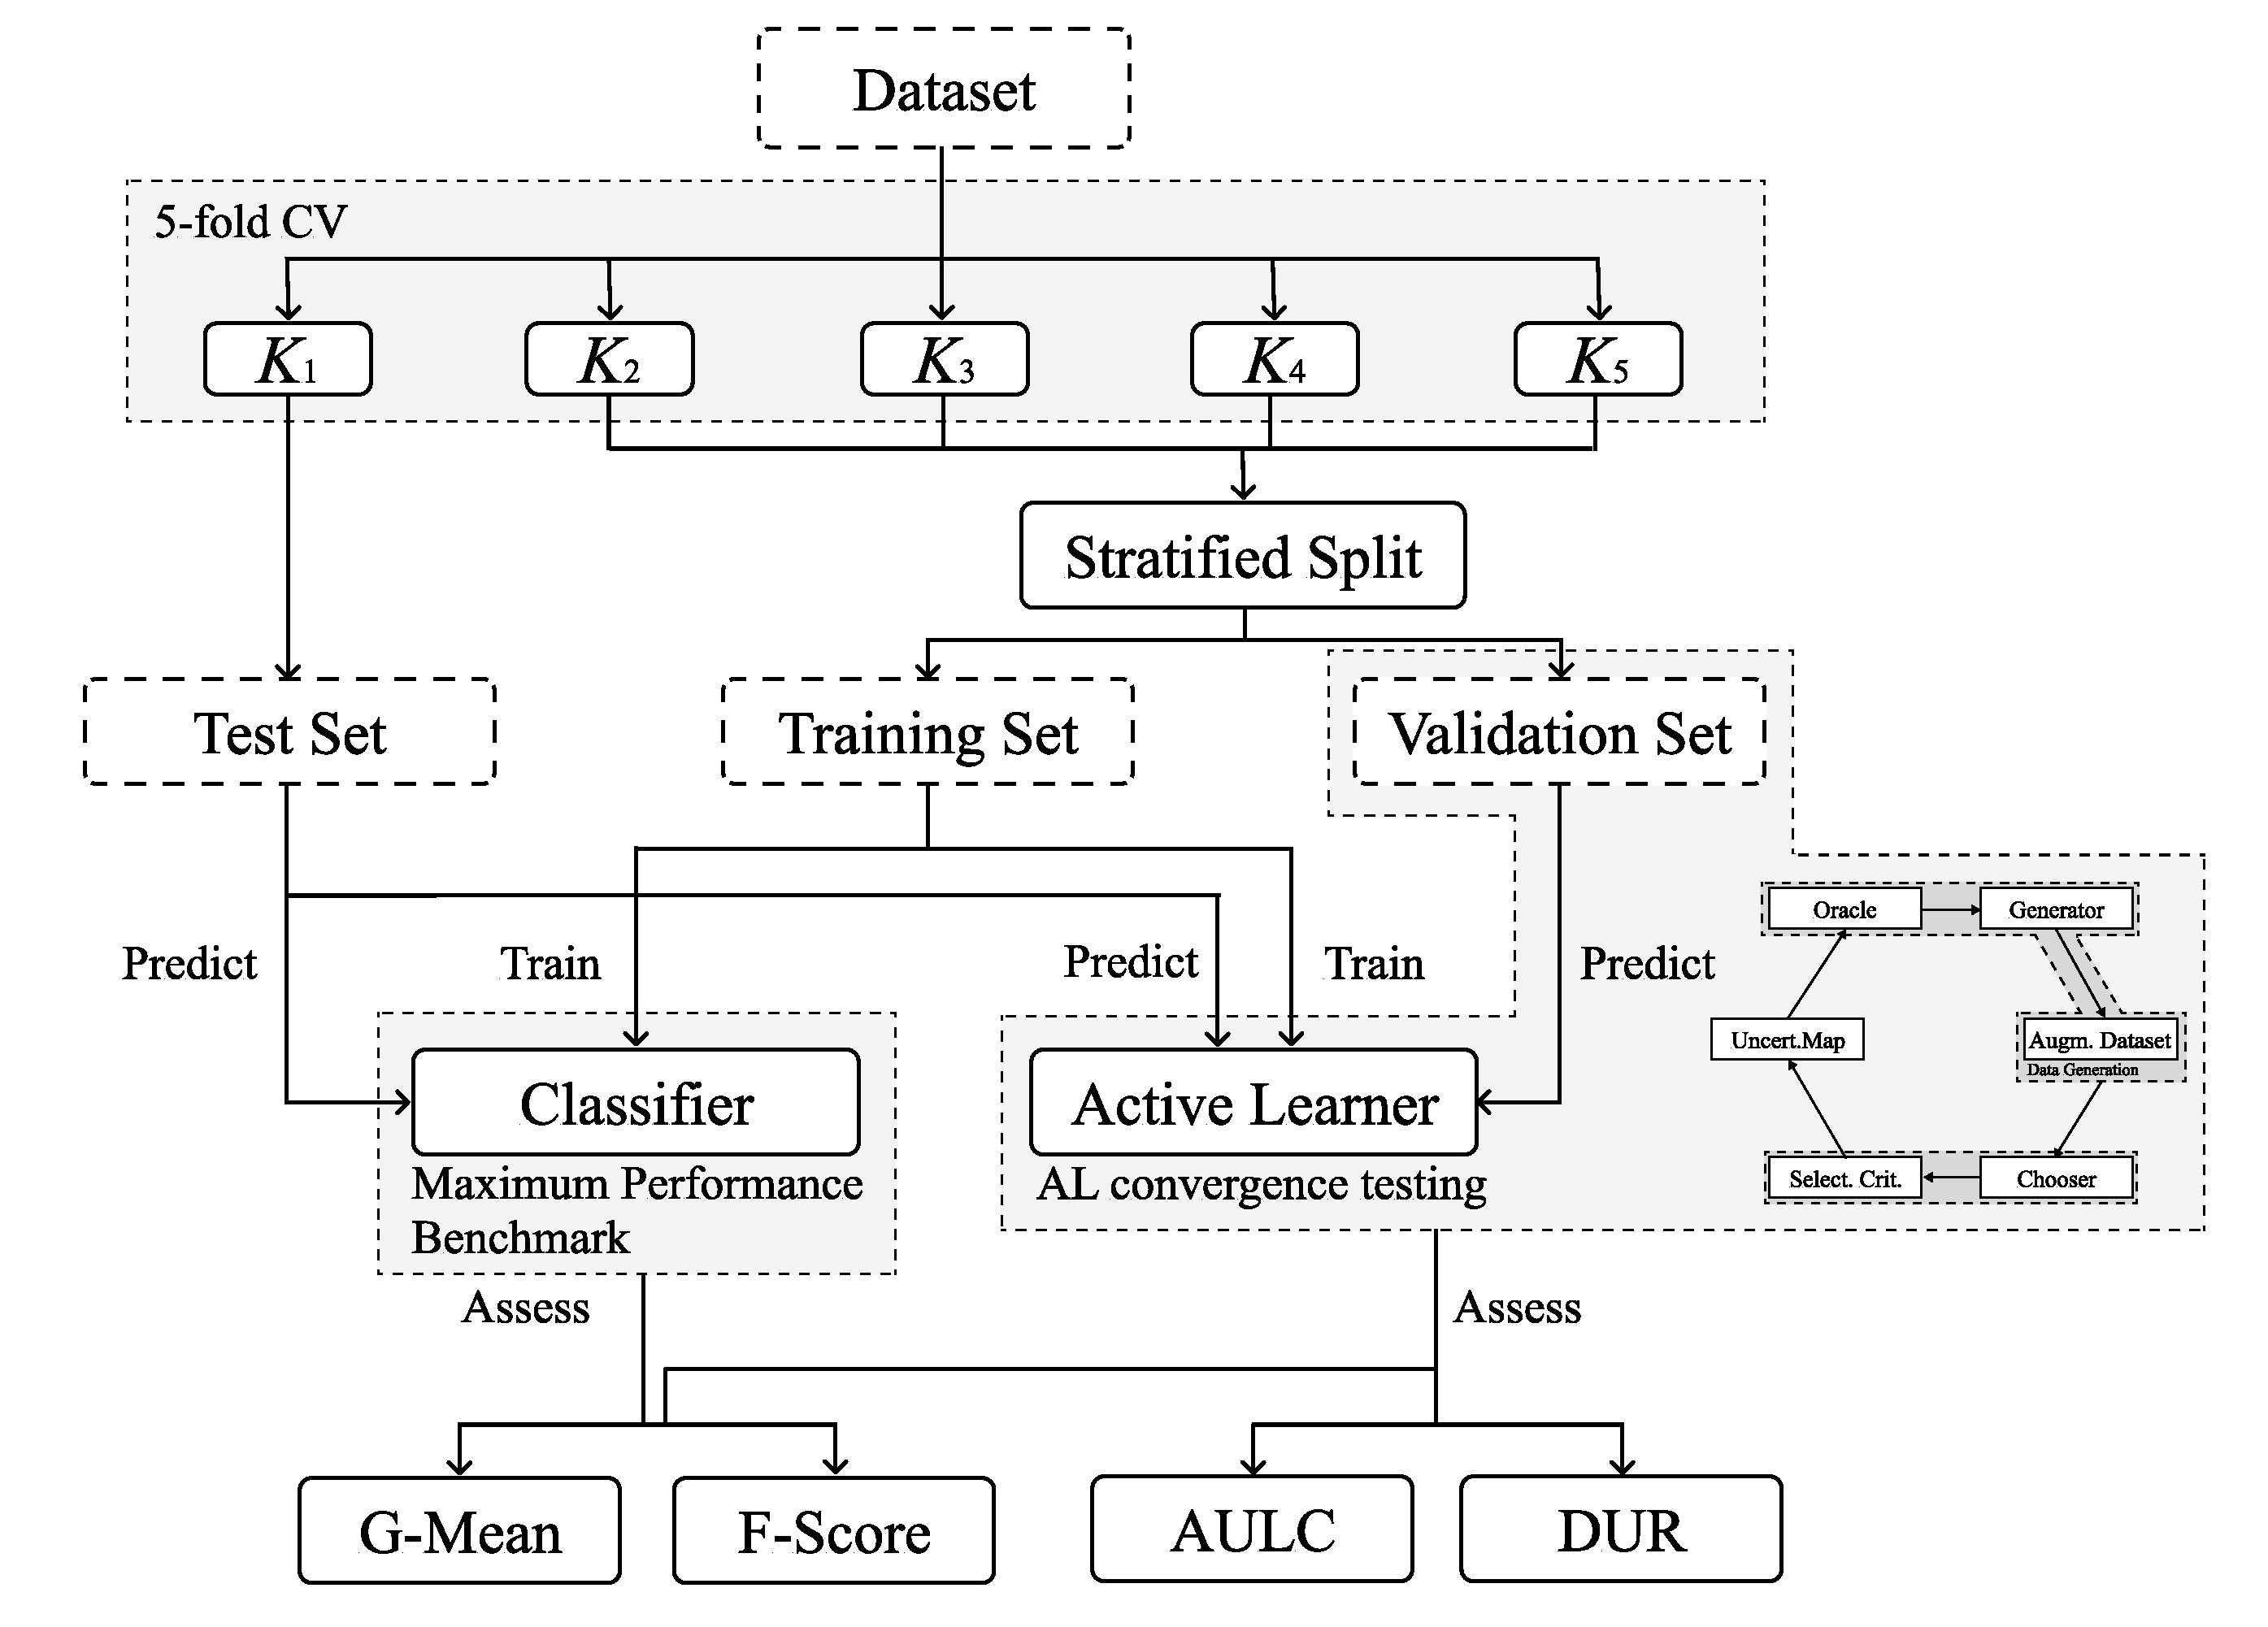
\includegraphics[width=.65\linewidth]{experiment_pipeline}
    \caption[Experimental procedure.]{%
        Experimental procedure. The datasets extracted from hyperspectral
        scenes are split in 5 folds. 1 of those (\textit{e.g.}, $K_1$) is used
        to test the optimal performance of AL algorithms and the
        classification without AL. The training set is used to iterate AL
        algorithms and train classifiers. The validation set is used to test
        the convergence of AL algorithms. The results are averaged over the 5
        folds across each of the 3 different initializations of this
        procedure.
    }~\label{fig:experiment_pipeline_al_generator}
\end{figure}

To make the AL-specific metrics comparable among active learners, the
configurations of the different frameworks must be similar. For each dataset,
the number of instances is constant to facilitate the analysis of the same
metrics. 

In most practical AL applications it is assumed that the number of instances 
in the initial training sample is too small to perform hyperparameter tuning.
Consequently, in order to ensure realistic results, our experimental procedure
does not include hyperparameter optimization. The predefined hyperparameters
are shown in Table~\ref{tab:grid_al_generator}. They were set up based on general
recommendations and default settings for the classifiers and generators used.

The AL iterative process is set up with a randomly selected initial training
sample with 15 initial samples. At each iteration, 15 additional samples are
added to the training set. This process is stopped after 49 iterations, once
50\% of the entire dataset (\textit{i.e.,} 78\% of the training set) is added
to the augmented dataset.

\begin{table}
	\centering
	\begin{tabular}{lll}
		\toprule
		Classifier & Hyperparameters      & Values             \\
		\midrule
		LR         & maximum iterations   & 10000              \\
		           & solver               & sag                \\
                   & penalty              & None               \\
		KNN        & \# neighbors         & 5                  \\
                   & weights              & uniform            \\
                   & metric               & euclidean          \\
		RF         & maximum tree depth   & None               \\
		           & \# estimators        & 100                \\
                   & criterion            & gini               \\
		\toprule
		Generator  &                      &                    \\
		\midrule
		G-SMOTE    & \# neighbors         & 5                  \\
                   & deformation factor   & 0.5                \\
                   & truncation factor    & 0.5                \\
		\bottomrule
	\end{tabular}
    \caption{Hyper-parameter definition for the classifiers and
    generator used in the experiment.}~\label{tab:grid_al_generator}
\end{table}

\subsection{Software Implementation}

The experiment was implemented using the Python programming language, along
with the Python libraries
\href{https://scikit-learn.org/stable/}{Scikit-Learn}~\cite{Pedregosa2011},
\href{https://imbalanced-learn.org/en/stable/}{Imbalanced-Learn}~\cite{JMLR:v18:16-365},
\href{https://geometric-smote.readthedocs.io/en/latest/?badge=latest}{Geometric-SMOTE},
\href{https://cluster-over-sampling.readthedocs.io/en/latest/?badge=latest}{Cluster-Over-Sampling}
and
\href{https://research-learn.readthedocs.io/en/latest/?badge=latest}{Research-Learn}
libraries. All functions, algorithms, experiments and results are provided in
the \href{https://github.com/joaopfonseca/publications/}{GitHub repository of the
project}.

\section{Results \& Discussion}~\label{sec:results-al-generator}

The evaluation of the different AL frameworks in a multiple dataset context
should not rely uniquely on the mean of the performance metrics across
datasets.~\cite{Demsar2006} recommends the use of mean ranking scores, since
the performance levels of the different frameworks varies according to the
data it is being used on. Consequently, evaluating these performance metrics
solely based on their mean values might lead to inaccurate analyses.
Accordingly, the results of this experiment are analysed using both the mean
ranking and absolute scores for each model. The rank values are assigned based
on the mean scores resulting from three different initializations of 5-fold
cross validation for each classifier and active learner. The goal of this
analysis is to understand whether the proposed framework (AL with the
integration of an artificial data generator) is capable of using less data
from the original dataset while simultaneously achieving better classification
results than the standard AL framework, \textit{i.e.}, guarantee a faster
classification convergence. 

\subsection{Results}~\label{sec:sub_results-al-generator}

Table~\ref{tab:aulc_ranks_al_generator} shows the average rankings and standard deviations
across datasets of the AULC scores for each active learner.

\begin{table}
    \centering
    \pgfplotstabletypeset[
        col sep=comma,
        string type,
        every head row/.style={%
            before row=\toprule,
            after row=\midrule
        },
        every last row/.style={after row=\bottomrule},
    ]{figures/al-generator-lulc/mean_std_aulc_ranks.csv}
    \caption[Mean rankings of the AULC metric.]{%
        Mean rankings of the AULC metric over the different datasets (7),
        folds (5) and runs (3) used in the experiment. This means that the use
        of G-SMOTE almost always improves the results of the original
        framework.
    }\label{tab:aulc_ranks_al_generator}
\end{table}

The mean AULC absolute scores are provided in Table~\ref{tab:aulc_scores_al_generator}.
These values are computed as the mean of the sum of the scores of a specific
performance metric over all iterations (for an AL configuration). In other
words, these values correspond to the average AULC over $7\ datasets \times 5\
folds \times 3\ initializations$.

\begin{table}
    \centering
    \pgfplotstabletypeset[
        col sep=comma,
        string type,
        every head row/.style={%
            before row=\toprule,
            after row=\midrule
        },
        every last row/.style={after row=\bottomrule},
    ]{figures/al-generator-lulc/mean_std_aulc_scores.csv}
    \caption[Average AULC of each AL configuration tested.]{%
        Average AULC of each AL configuration tested. Each AULC score is
        calculated using the G-mean scores of each iteration in the validation
        set. By the end of the iterative process, each AL configuration used a
        total of 750 instances of the 960 instances that compose the training
        set.
    }~\label{tab:aulc_scores_al_generator}
\end{table}

The average DURs are shown in Table~\ref{tab:optimal_data_utilization_al_generator}. They
were calculated for various G-mean scores thresholds, varying at a step of 5\%
between 60\% and 95\%. Each row shows the percentage of training data required
by the different AL configurations to reach that specific G-mean score.

\pgfplotstabletypeset[
	begin table=\begin{longtable},
	end table=\end{longtable},
	col sep=comma,
	header=true,
    columns={G-mean Score,Classifier,Standard,Proposed}, 
    string type,
    every head row/.style={before row=\toprule, after row=\midrule\endhead},
	every last row/.style={
        after row={
            \bottomrule
            \caption[Mean data utilization of AL algorithms.]{
                Mean data utilization of AL algorithms, as a percentage of the training set.
            }~\label{tab:optimal_data_utilization_al_generator}
        }
    }
]{figures/al-generator-lulc/optimal_data_utilization.csv}

The DUR of the proposed method relative to the baseline method is shown in
Figure~\ref{fig:dur_al_generator}. A DUR below 1 means that the proposed framework requires
less data to reach the same performance threshold (as a percentage, relative
to the amount of data required by the baseline framework). For instance, in the
upper left graphic we can see that the proposed framework achieves 90\%
classification using F-score while using 91\% of the amount of data used by the
traditional AL framework, in other words 9\% less data.

\begin{figure}
	\centering
	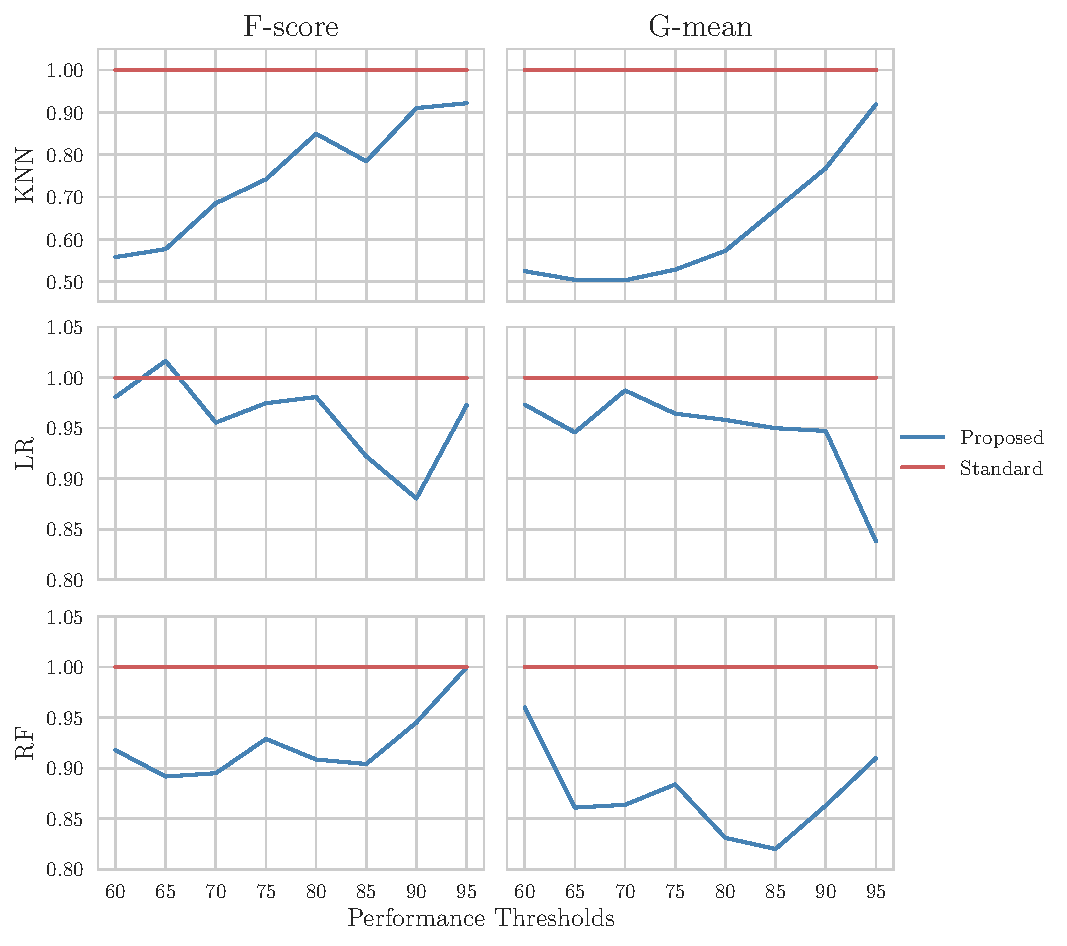
\includegraphics[width=.75\linewidth]{data_utilization_rate}
    \caption[Mean data utilization rates.]{%
        Mean data utilization rates. The y-axis shows the percentage of data
        (relative to the baseline AL framework) required to reach the
        different performance thresholds.
    }~\label{fig:dur_al_generator}
\end{figure}

The averaged optimal classification scores are shown in
Table~\ref{tab:optimal_mean_std_scores_al_generator}. The maximum performance (MP)
classification scores are shown as a benchmark and represent the performance
of the corresponding classifier using the entire training set. 

\begin{table}
    \centering
    \addtolength{\leftskip} {-2cm}
    \addtolength{\rightskip}{-2cm}
    \pgfplotstabletypeset[
        col sep=comma,
        string type,
        every head row/.style={%
            before row=\toprule,
            after row=\midrule
        },
        every last row/.style={after row=\bottomrule},
    ]{figures/al-generator-lulc/optimal_mean_std_scores.csv}
    \caption[Optimal classification scores.]{%
        Optimal classification scores. The Maximum Performance (MP)
        classification scores are calculated using classifiers trained using
        the entire training set.
    }~\label{tab:optimal_mean_std_scores_al_generator}
\end{table}

\subsection{Statistical Analysis}~\label{sec:statistical-analysis-al-generator}

The methods used to test the experiment's results must be appropriate for a
multi-dataset context. Therefore the statistical analysis is performed using
the Wilcoxon signed-rank test~\cite{Wilcoxon1945} as a post-hoc analysis. The
variable used for this test is the data utilization rate based on the
G-mean performance metric, considering the various performance thresholds
from Table~\ref{tab:optimal_data_utilization_al_generator}.

The Wilcoxon signed-rank test results are shown in
Table~\ref{tab:wilcoxon_test}. We test as null hypothesis that the performance
of the proposed framework is the same as the original AL framework. The null
hypothesis was rejected in all datasets.

\begin{table}
	\centering
    \pgfplotstabletypeset[
        col sep=comma,
        string type,
        every head row/.style={%
            before row=\toprule,
            after row=\midrule
        },
        every last row/.style={after row=\bottomrule},
    ]{figures/al-generator-lulc/wilcoxon_test.csv}
    \caption[Adjusted p-values using the Wilcoxon signed-rank method.]{%
    	Adjusted p-values using the Wilcoxon signed-rank method. Bold values
        are statistically significant at a level of $\alpha = 0.05$. The 
        null hypothesis is that the performance of the proposed
        framework is similar to that of the original framework.
    }\label{tab:wilcoxon_test}
\end{table}

\subsection{Discussion}

This paper expands the AL framework by adding an artificial data generator
into its iterative process. This modification is done to accelerate the
classification convergence of the standard AL procedure, which is
reflected in the reduction of the amount of data necessary to reach better
classification results.

The convergence efficiency of the proposed method is always higher than the
baseline AL framework, with the exception of one comparison, as shown in
Table~\ref{tab:aulc_ranks_al_generator} and Figure~\ref{fig:dur_al_generator}. This means the proposed
AL framework using data generation was able to outperform the baseline AL in
nearly all scenarios. 

The mean AULC scores in Table~\ref{tab:aulc_scores_al_generator} show a significant
improvement in the performance of AL when a generator is used. The mean
performance of the proposed framework is always better than the
baseline framework. This improvement is explained by:

\begin{enumerate}
    \item Earlier convergence of AL, \textit{i.e.}, requiring less data to
        achieve comparable performance levels. This effect is shown in
        Table~\ref{tab:optimal_data_utilization_al_generator}, where we found that the
        proposed framework always uses less data for similar performance
        levels, regardless of the classifier used.
    \item Higher optimal classification performance, \textit{i.e.}, reaching
        higher performance levels overall. This effect is shown in
        Table~\ref{tab:optimal_mean_std_scores_al_generator}, where we found that using a
        generator in AL led to a better classification performance and was
        capable of outperforming the MP threshold. 
\end{enumerate} 

Our results show statistical significance in every dataset. The proposed
framework had a superior performance with statistical significance on each
dataset at a level of $\alpha = 0.05$. This indicates that regardless of the
context under which an AL algorithm is used, the proposed framework reduces
the amount of data necessary in the AL's iterative process.

This paper introduces the concept of applying data a generation algorithm in
the AL framework. This was done with the implementation of a recent state of
the art generalization of a popular data generation algorithm. Although, since
this algorithm is based on heuristics, future work should focus on improving
these results through the design of new data generation mechanisms, at the
cost of additional computational power. In addition, we also noticed
significant standard errors in our experimental results
(see Subsection~\ref{sec:sub_results-al-generator}). This indicates that
AL procedures seem to be particularly sensitive to the initialization method,
which is still a limitation of AL, regardless of the framework and
configurations used. This is consistent with the findings
in~\cite{Kottke2017}, which future work should attempt to address. Although
using a generator marginally reduced this standard error, it is not sufficient
to address this specific limitation.

\section{Conclusion}~\label{sec:conclusion-al-generator}

The aim of this experiment was to test the effectiveness of a new AL framework
that introduces artificial data generation in its iterative process. The
experiment was designed to test the proposed method under particularly
challenging conditions, where the maximum performance line is naturally high
in most datasets. The element that constitute the Generator component was set
up in a plug-and-play scheme, without significant tuning of the G-SMOTE
oversampler. Using a generator in AL improved the original AL framework in all
scenarios. These results could be further improved through the modification
and more intense tuning of the data generation strategy. In our experiment,
artificial data was generated only to match each non-majority class frequency
with the majority class frequency, strictly balancing the class distribution.
Generating a larger amount of data for all classes can further improve these
results. 

The high performance scores for the baseline AL framework made the achievement
of significant improvements over the traditional AL framework under these
conditions particularly meaningful. The advantage of the proposed AL framework
is shown in Table~\ref{tab:optimal_data_utilization_al_generator}. In most of the presented
scenarios there is a substantial reduction of data necessary to reach a given
performance threshold. 

The results from this experiment show that using a data generator in the AL
framework will improve the convergence of the method. This framework
successfully anticipate the predictor's optimal performance, as shown in
Tables~\ref{tab:aulc_ranks_al_generator},~\ref{tab:aulc_scores_al_generator}
and~\ref{tab:optimal_data_utilization_al_generator}. Therefore, in a real application, the
annotation cost would have been reduced since less iterations and labeled
instances are necessary to reach near optimal classification performance.

\thesischapter{%
    Improving Active Learning Performance Through the Use of Data Augmentation
}{%
    Published as Joao Fonseca, Fernando Bacao, in International Journal of
    Intelligent Systems, 2023
}~\label{chp:active-learning-augmentation}
\graphicspath{{figures/active-learning-augmentation/}}

\begin{adjustwidth}{30pt}{30pt}

    Active Learning (AL) is a well-known technique to optimize data usage in
    training, through the interactive selection of unlabeled observations, out
    of a large pool of unlabeled data, to be labeled by a supervisor. Its
    focus is to find the unlabeled observations that, once labeled, will
    maximize the informativeness of the training dataset, therefore reducing
    data related costs. The literature describes several methods to improve
    the effectiveness of this process. Nonetheless, there is a paucity of
    research developed around the application of artificial data sources in
    AL, especially outside image classification or NLP. This paper
    proposes a new AL framework, which relies on the effective use of
    artificial data. It may be used with any classifier, generation mechanism
    and data type, and can be integrated with multiple other state-of-the-art
    AL contributions. This combination is expected to increase the ML
    classifier's performance and reduce both the supervisor's involvement and
    the amount of required labeled data, at the expense of a marginal increase
    in computational time. The proposed method introduces a
    hyperparameter optimization component to improve the generation of
    artificial instances during the AL process, as well as an
    uncertainty-based data generation mechanism. We compare the proposed
    method to the standard framework and an oversampling-based active
    learning method for more informed data generation in an AL context.
    The models' performance was tested using four different classifiers, two
    AL-specific performance metrics and three classification performance
    metrics over 15 different datasets. We demonstrate that the proposed
    framework, using data augmentation, significantly improves the performance
    of AL, both in terms of classification performance and data selection
    efficiency.\footnote{All the code and preprocessed data developed for
        this study is available at
        https://github.com/joaopfonseca/publications/.
    } 

\end{adjustwidth}

\vspace{.5cm}
\textbf{Keywords:} Active Learning; Data Augmentation; Oversampling


\section{Introduction}~\label{sec:introduction-al-aug}

The importance of training robust ML models with minimal data
requirements is substantially increasing~\cite{Nath2021, Sverchkov2017,
Li2012}. Although the growing amount of valuable data sources and formats
being developed and explored is affecting various domains~\cite{Li2021}, this
data is often unlabeled. Only a tiny amount of the data being produced and
stored can be helpful in supervised learning tasks. In addition, it is often
difficult and expensive to label data for specific Machine Learning (ML)
projects, especially when data-intensive ML techniques are involved
(\textit{e.g.,} Deep Learning classifiers)~\cite{Nath2021}. In this scenario,
labeling the full dataset becomes impractical, time-consuming and expensive.
Two different ML techniques attempt to address this problem: Semi-Supervised
Learning (SSL) and Active Learning (AL). Even though they address the same
problem, the two follow different approaches. SSL focuses on observations with
the most certain predictions, whereas AL focuses on observations with the
least certain predictions~\cite{Simeoni2020}.

SSL attempts to use a small, predefined set of labeled and unlabeled data to
produce a classifier with superior performance. This method uses the unlabeled
observations to help define the classifier's decision
boundaries~\cite{Van2020}. Simultaneously, the amount of labeled data required
to reach a given performance threshold is also reduced. It is a particular
case of ML because it falls between the supervised and unsupervised learning
perspectives. AL, instead of optimizing the informativeness of an existing
training set, expands the dataset to include the most informative and/or
representative observations~\cite{Sener2018}. It is an iterative process where
a supervised model is trained and simultaneously identifies the most
informative unlabeled observations to increase the performance of that
classifier. The combination of SSL with AL has been explored in the past,
achieving state-of-the-art results~\cite{Leng2013}.
 
Several studies have pointed out the limitations of AL within an Imbalanced
Learning context~\cite{Yu2019, zhang2020reinforcement}. With imbalanced data,
AL approaches frequently have low performance, high computational time, or
data annotation costs.  Studies addressing this issue tend to adopt
classifier-level modifications, such as the Weighted Extreme Learning
Machine~\cite{Yu2019, Zong2013, Qin2021}. However, classifier or query
function-level modifications (See Section~\ref{sec:active_learning_methods-al-aug})
have limited applicability since a universally good AL strategy has not yet
been found~\cite{Sener2018}. Other methods address imbalanced learning by
weighing the observations as the function of the observation's class imbalance
ratio~\cite{Liu2021}. Alternatively, other techniques reduce the imbalanced
learning bias by combining Informative and Representative-based query
approaches (see Section~\ref{sec:active_learning_methods-al-aug})~\cite{Tharwat2020}.
Another approach to deal with imbalanced data and data scarcity, in general,
is generating synthetic data~\cite{He2009}. This approach has the
advantage of being classifier-agnostic, it potentially reduces the imbalanced
learning bias, and also works as a regularization method in data-scarce
environments, such as AL implementations~\cite{Kim2021}. However, most recent
studies improve the AL performance by modifying the design/choice of the
classifier and query functions used.

Recently, synthetic data generation techniques gathered attention among ML
researchers for its effectiveness over a wide range of applications:
regularization, oversampling, semi-supervised learning, self-supervised
learning, etc. Data augmentation generates synthetic observations to
complement naturally occurring observations. It aims to reinforce the
definition of a ML classifier's decision boundary during the learning phase
and improve the generalization of the algorithm. These techniques have the
advantage of being a data level technique (despite the existence of
augmentation methods applied internally in the ML classifier). Therefore, they
can be implemented in a way that will not affect the choice of classifier and
does not exclude the usage of other regularization approaches. In an AL
context, the generation of synthetic data becomes particularly appealing,
especially with randomized and statistical-based approaches; it ensures better
model performance with reduced involvement of a human agent, at the expense of
a marginal increase in computational power. In addition, synthetic data is
expected to reduce the amount labeled data required for a good AL
implementation.

\begin{figure}[t]
	\centering
	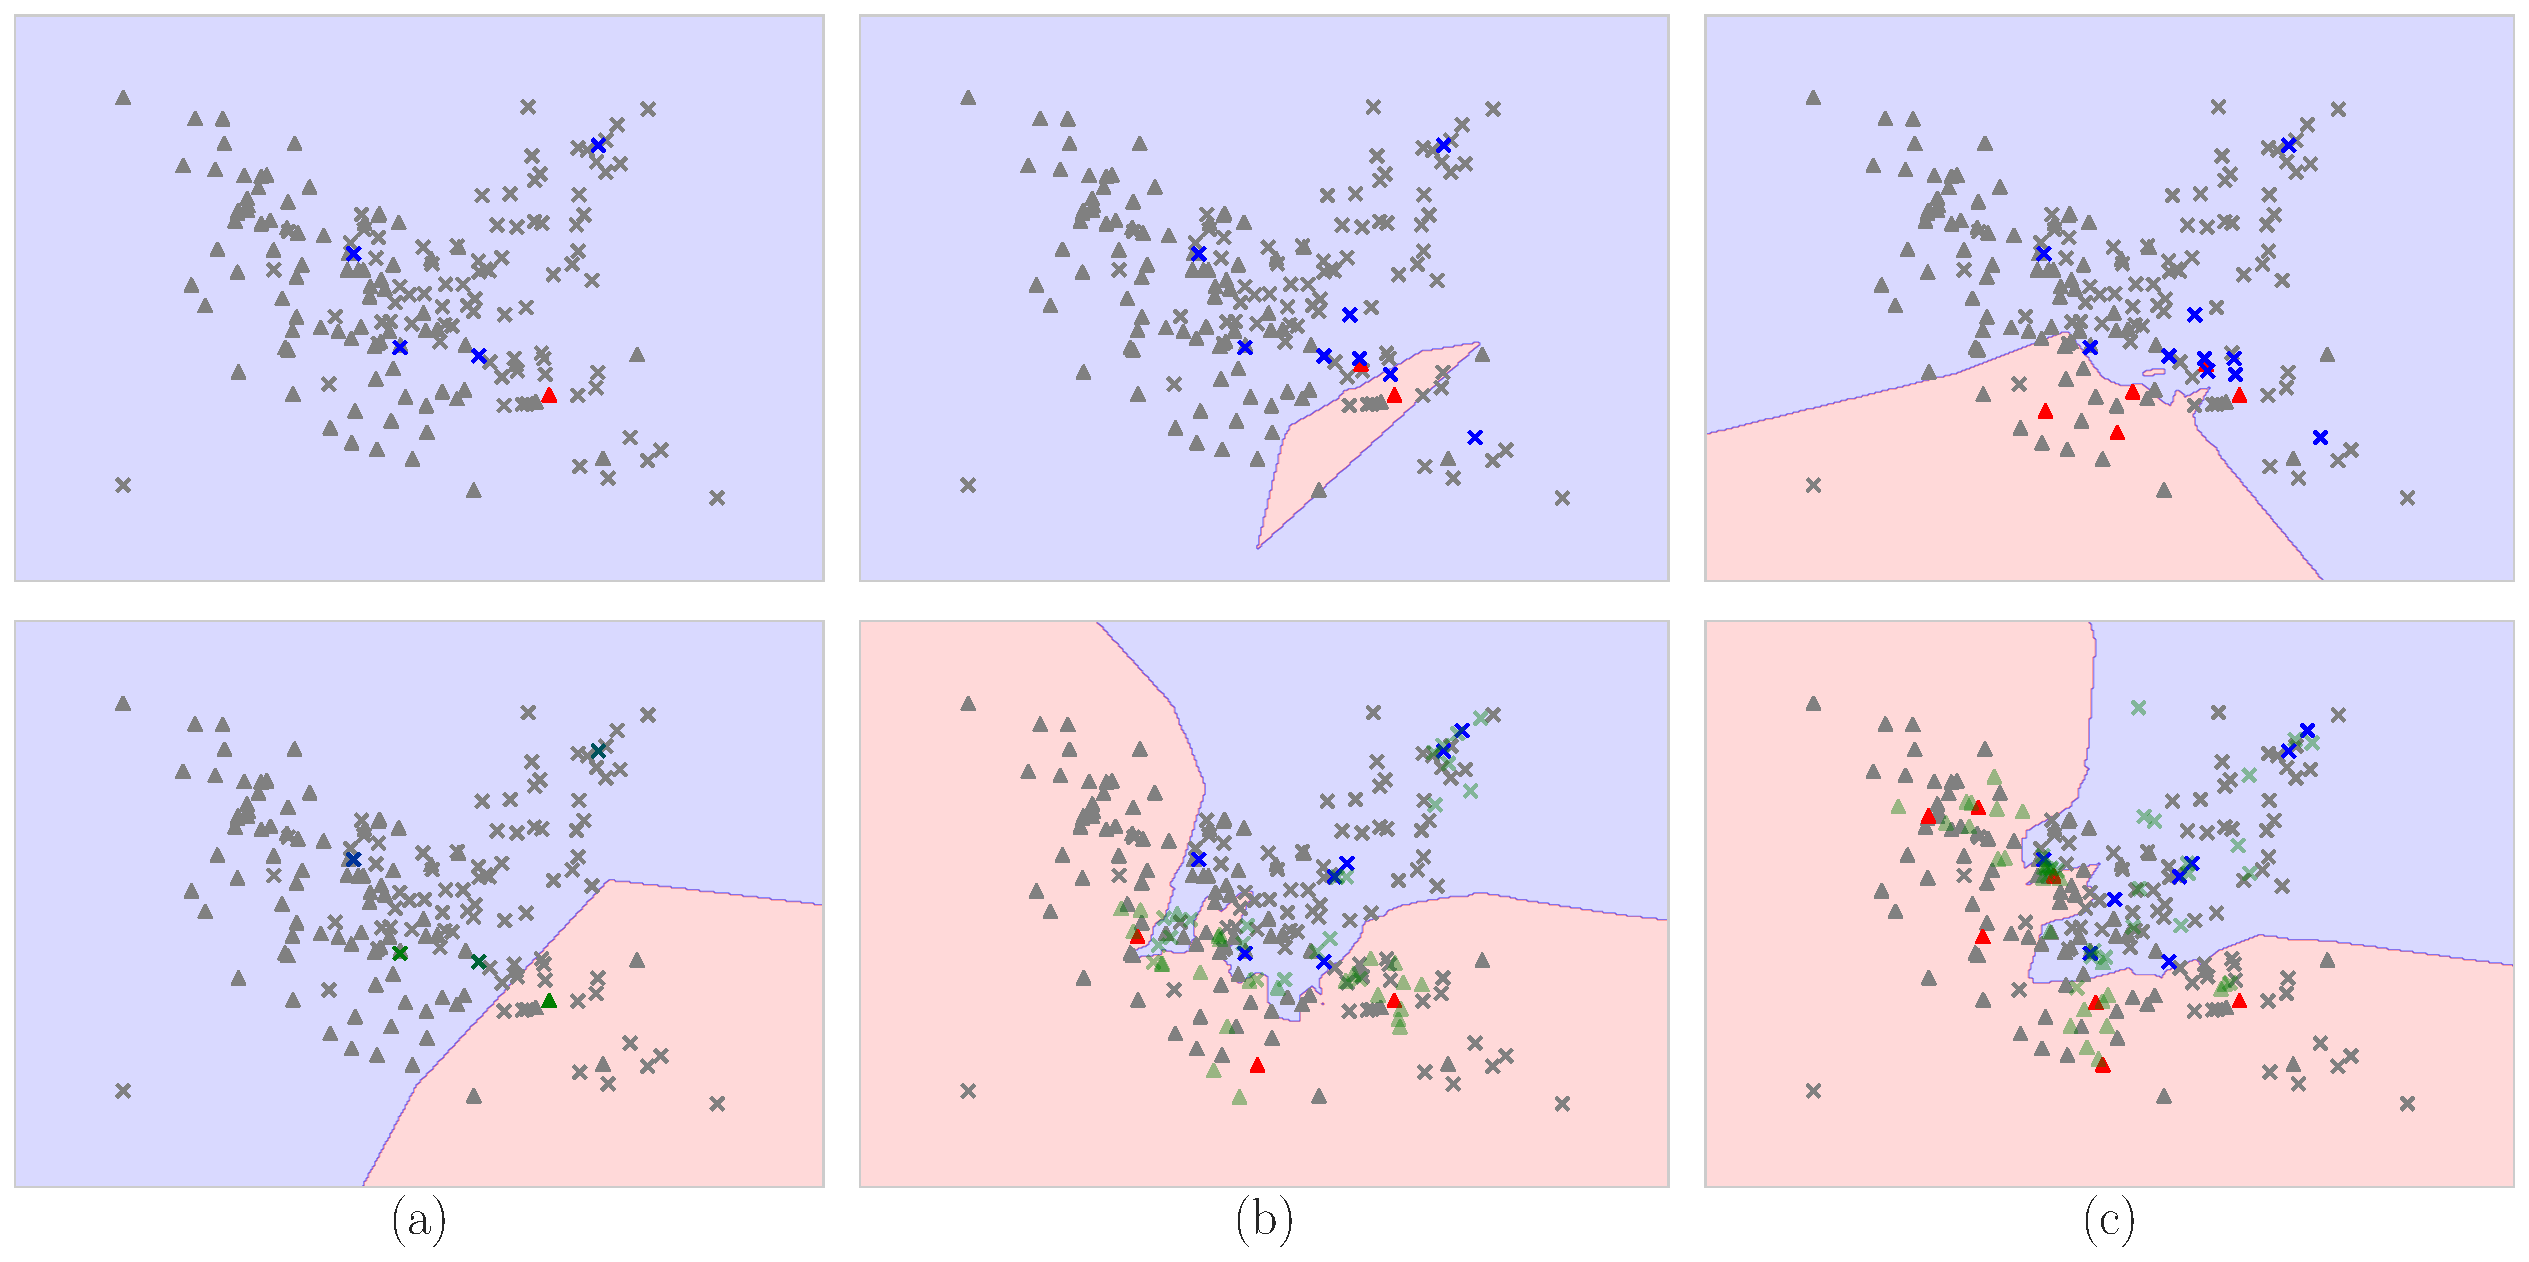
\includegraphics[width=\linewidth]{al-example}
    \caption{%
        Illustration of the different acquisition processes in AL using a
        K-Nearest Neighbors classifier and Shannon's entropy as the
        uncertainty estimation function, with five observations being
        collected and labeled per iteration. The top row shows the behavior of
        a standard AL implementation, while the bottom row shows the behavior
        of the proposed method. Column (a), (b) and (c) show the decision
        boundaries at iterations 1 (after the collection of five random initial training
        observations), 2 (with 10 labeled observations) and 3 (with 15 labeled
        observations), respectively. The initial labeled dataset for both approaches is
        the same. The two classes are distinguished with $\triangle$ and
        $\times$, and are colored as red and blue (respectively) if they are
        labeled. The transparent green observations are synthetic observations
        (bottow row only).
    }~\label{fig:al-example}
\end{figure}

Figure~\ref{fig:al-example} illustrates the difference across AL
iterations between the standard AL approach and the proposed method. Synthetic
data allowed for a quicker expansion of the labeled input area at an early
stage of the process, with better defined decision boundaries and
near-covergence of the ML classifier's performance at the third iteration.
Data augmentation influences the choice of unlabeled observations for labeling
into regions where synthetic data is not being able to represent the unlabeled
data pool.
 
\subsection{Motivation and contributions}

The usage of data augmentation in AL is not new. The literature found on the
topic (see Section~\ref{sec:data_augmentation_in_al-al-aug}) focuses on either image
classification or Natural Language Processing and uses Deep Learning-based
data augmentation to improve the performance of neural network architectures
in AL\@. These methods, although showing promising results, represent a
limited perspective of the potential of data augmentation in a real-world
setting: 

\begin{enumerate}

    \item Using Deep Learning in an iterative setting requires access to
        significant computational power.

    \item These models tend to use sophisticated data augmentation methods,
        whose implementation may not be accessible to non-sophisticated users.

    \item They require a significant amount of processing time per
        iteration and are inappropriate for settings with limited time
        budgets.

    \item The studies found on the topic are specific to the domain,
        classifier, and data augmentation method.
        In addition, all of the related methods found (except one) focus
        on either image or natural language processing classification
        problems.

\end{enumerate}

Consequently, the direct effect of data augmentation is unclear: these studies
implement different neural network-based techniques for different
classification problems, whose performance may be attributed to various
elements within the AL framework.

In this study, we explore the effect of data augmentation in AL in a
context-agnostic setting, along with two different data augmentation policies:
oversampling (where the amount of data generated for each class equals the
amount of data belonging to the majority class) and non-constant data
augmentation policies (where the amount of data generated exceeds the amount
of data belonging to the majority class in varying quantities) between
iterations. We start by conceptualizing the AL framework and each of its
elements, as well as the modifications involved to implement data augmentation
in the AL iterative process. We argue that simple, non-domain specific data
augmentation heuristics are sufficient to improve the performance of AL
implementations, without the need to resort to deep learning-based data
augmentation algorithms. These contributions can be summarized as
follows:

\begin{enumerate}

    \item We propose a flexible AL framework with pipelined data
        augmentation for tabular data that may be adapted for any domain or
        data type. This implementation is directed towards use cases with
        limited computational power and/or processing time.

    \item We use a geometric-based data augmentation method for
        non-network based classifiers and adapt it to leverage information
        from the AL process. To the best of our knowledge, most
        existing methods use domain/classifier-specific augmentations or the
        Mixup approach, which is incompatible with most classifiers that are
        not neural network-based.

    \item We provide empirical evidence that the integration of varying data
        augmentation policies between iterations in the AL framework not only further
        reduces the amount of labeled data required, but is also a viable training
        strategy for fully supervised learning settings.

\end{enumerate}

When compared to the standard AL framework, the proposed framework contains
two additional components: the Generator and the Hyperparameter Optimizer. We
implement a modified version of the Geometric Synthetic Minority Oversampling
Technique (G-SMOTE)~\cite{Douzas2019} as a data augmentation method with an
optimized generation policy (explained in
Section~\ref{sec:data_augmentation}). We also propose a hyperparameter
optimization module, which is used to find the best data augmentation policy
at each iteration. We test the effectiveness of the proposed method in 15
datasets of different domains. We implement three AL frameworks (standard,
oversampling and varying data augmentation) using four different classifiers,
three different performance metrics and calculate two AL-specific performance
metrics. 

The remainder of this manuscript is structured as follows:
Section~\ref{sec:background-al-aug} introduces relevant topics discussed in the paper
and describes the related work. Section~\ref{sec:proposed_method-al-aug} elucidates
the proposed method. Section~\ref{sec:methodology-al-aug} details the methodology of
the study's experiment. Section~\ref{sec:results_discussion-al-aug} presents the
results obtained from the experiment, as well as a discussion of these
results. Section~\ref{sec:conclusion-al-aug} presents the conclusions drawn from
this study.
 
\section{Background}~\label{sec:background-al-aug}

In this section we describe the AL problem, data augmentation techniques, and review the
literature that combines AL with data augmentation. Table~\ref{tbl:generators}
describes the notations used throughout the rest of this study.

\begingroup\small
\begin{longtable}{clccccccc}
    \caption{%
        Description of all notations and symbols used throughout the
        manuscript.
    }\label{tbl:generators}\\
    \toprule
               Symbol & Meaning \\
    \midrule
    \endfirsthead%
    \caption[]{%
        Description of all notations and symbols used throughout the
        manuscript.
    } \\
    \toprule
               Symbol & Meaning \\
    \midrule
    \endhead%
    \midrule
    \multicolumn{9}{r}{{Continued on next page}} \\
    \midrule
    \endfoot%
    
    \bottomrule
    \endlastfoot%
               $f_{c}$ & ML classifier. \\
               $x_i$ & Observation at index $i$. \\
               $f_{acq}(x_i;f_c)$ & Acquisition function. \\
               $f_{aug}(x_i;\tau)$ & Augmentation function. \\
               $\tau$ & Augmentation policy. \\
               $\mathcal{D}$ & Data pool. Contains both labeled and unlabeled
                               data. \\
               $\mathcal{D}_{lab}^t$ & Labeled data set at iteration $t$. \\
               $\mathcal{D}_{pool}^t$ & Unlabeled data pool at iteration $t$. \\
               $\mathcal{D}_{new}^t$ & Set of observations from
                                       $\mathcal{D}_{pool}^t$to be labeled
                                       and added to $\mathcal{D}_{lab}^{t+1}$. \\
               $T$ & Iteration budget.\\
               $n$ & Annotation budget per iteration.\\
\end{longtable}
\endgroup


\subsection{Active Learning}~\label{sec:active_learning_methods-al-aug}

This paper focuses on pool-based AL methods as defined
in~\cite{katz2021improved}. The goal of AL models is to maximize the
performance of a classifier, $f_{c}$, while annotating as least observations,
$x_i$, as possible. They use a data pool, $\mathcal{D}$, where $\mathcal{D} =
\mathcal{D}_{lab} \cup \mathcal{D}_{pool}$ and $|\mathcal{D}_{pool}| \gg
|\mathcal{D}_{lab}|$. $\mathcal{D}_{pool}$ and $\mathcal{D}_{lab}$ refer to
the sets of unlabeled and labeled data, respectively. Having a budget of $T$
iterations (where $t \in \{1, 2, \ldots, T\}$) and $n$ annotations per iteration, at
iteration $t$, $f_c$ is trained using $\mathcal{D}_{lab}^t$ to produce, for
each $x_i \in \mathcal{D}_{pool}^t$, an uncertainty score using an acquisition
function $f_{acq}(x_i;f_c)$. These uncertainty scores are used to annotate the
$n$ observations with highest uncertainty from $\mathcal{D}_{pool}^t$ to form
$\mathcal{D}_{new}^t$. The iteration ends with the update of
$\mathcal{D}_{lab}^{t+1} = \mathcal{D}_{lab}^t \cup \mathcal{D}_{new}^t$ and
$\mathcal{D}_{pool}^{t+1} = \mathcal{D}_{pool}^t \setminus
\mathcal{D}_{new}^t$~\cite{Su2020, Sverchkov2017}. This process is shown in
Figure~\ref{fig:al_iteration}. Before the start of the iterative process,
assuming $\mathcal{D}_{lab}^{t=0} = \emptyset$, the data used to populate
$\mathcal{D}_{lab}^{t=1}$ is typically collected randomly from $\mathcal{D} =
\mathcal{D}_{pool}^{t=0}$ and is labeled by a supervisor~\cite{Fonseca2021al,
Yoo2019, Aghdam2019}. 

\begin{figure}[ht]
	\centering
	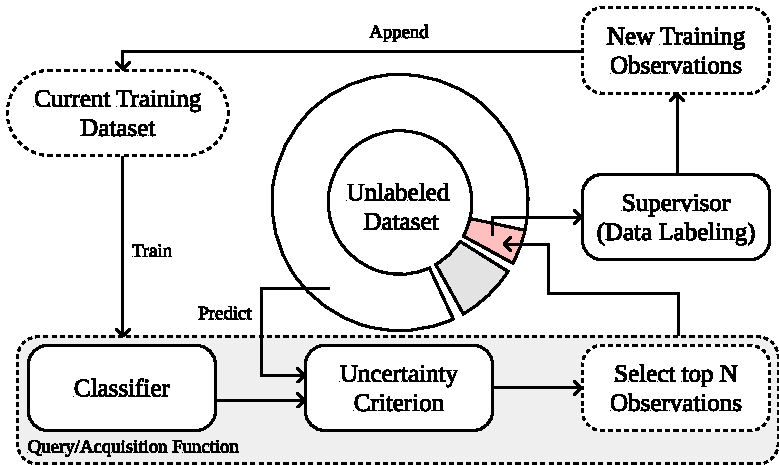
\includegraphics[width=.6\linewidth]{al_iteration}
    \caption{%
        Diagram depicting a typical AL iteration. In the first iteration, the
        training set collected during the initialization process becomes the
        ``Current Training Dataset''.
    }~\label{fig:al_iteration}
\end{figure}

Research focused on AL has typically been focused on the specification of
$f_{acq}$~\cite{hospedales2011finding} and domain-specific applications, such
as malware detection~\cite{li2022boosting} or Land Use/Land Cover
classification~\cite{li2020label}. Acquisition functions can be divided into
two different categories~\cite{su2021cost, Kumar2020}: 

\begin{enumerate}

    \item Informative-based. These strategies use the classifier's output to
        assess the importance of each observation towards the performance of
        the classifier~\cite{Fu2013}.

    \item Representative-based. These strategies estimate the optimal set of
        observations that will optimize the classifier's
        performance~\cite{Kumar2020}.

\end{enumerate}

Although there are significant contributions toward the development of more
robust query functions and classifiers in AL, modifications to AL's basic
structure are rarely explored. In~\cite{Yoo2019} the authors introduce a loss
prediction module in the AL framework to replace the uncertainty criterion.
This model implements a second classifier to predict the expected loss of the
unlabeled observations (using the actual losses collected during the training
of the original classifier) and return the unlabeled observations with the
highest expected loss. However, this contribution is specific to deep neural
networks and was only tested for image classification.


%%%%%%%%%%%%%%%%%%%%%%%%%%%%%%%%%%%%%%%%%%%%%%%%%%%%%%%%%%%%%%%%%%%%%%%%%%%%%%

AL techniques may also be used to complement other well-known learning
challenges. For example, security bug report prediction tasks are typically
developed in imbalanced learning environment, where it is necessary to
manually label large amounts of data, which may result in mislabeled
data~\cite{wu2021data}. Another related example is machinery fault
diagnostics, where the quality and quantity of the data collected is often
recognized as a bottleneck~\cite{zhang2023blockchain}. In this case,
ML-based techniques frequently leverage unlabeled data to improve the
classification performance~\cite{zhang2021open} and rely on manual data
acquisition~\cite{he2017deep}. In these examples, the application of an
AL technique could reduce the amount of labeled data required, reduce the
strain in the supervisor's labeling process and reduce the amount of label
noise. 

An under explored challenge in the AL literature is the effective handling of
different data structures. One method to address this problem are autoencoder
architectures~\cite{li2017grass} or, in the case of text data, semantic
representation networks~\cite{zheng2021sentence}. However, understanding
how to integrate these two types of methods is a subject of future research.
Within other research streams, such as deep reinforcement learning, some
research also focus on optimizing observation efficiency during the learning
process~\cite{zhang2022training}.

%%%%%%%%%%%%%%%%%%%%%%%%%%%%%%%%%%%%%%%%%%%%%%%%%%%%%%%%%%%%%%%%%%%%%%%%%%%%%%

\subsection{Data Augmentation}~\label{sec:data_augmentation-al-aug}

The standard AL model can be complemented with a data augmentation function,
$f_{aug}(x_i;\tau)$, where $\tau$ defines the augmentation policy. In this
context, $\tau$ refers to the transformation applied and its hyperparameters
and $f_{aug}$ produces a modified observation, $\tilde{x} \in
\mathcal{D}_{aug}$ where $\mathcal{D}_{aug}$ is the set of modified
observations. This involves the usage of a new set of data,
$\mathcal{D}_{train}^t = \mathcal{D}_{lab}^t \cup \mathcal{D}_{aug}^t$, to
train the classifier.

Data Augmentation methods expand the training dataset by introducing new and
informative observations \cite{Behpour2019}. The production of artificial data
may be done via the introduction of perturbations on the
input~\cite{Fonseca2021}, feature~\cite{DeVries2017}, or output
space~\cite{Behpour2019}. Data Augmentation methods may be divided into two
categories~\cite{Shorten2019}:

\begin{enumerate}
    \item Heuristic approaches attempt to generate new and relevant
        observations by applying a predefined procedure, usually incorporating
        some degree of randomness~\cite{Kashefi2020}. Since these methods
        typically occur in the input space, they require fewer data and
        computational power when compared to Neural Network methods. 
    \item Neural Network approaches, on the other hand, map the original input
        space into a lower-dimensional representation, known as the feature
        space~\cite{DeVries2017}. The generation of artificial data occurs in
        the feature space and is reconstructed into the input space. Although
        these methods allow the generation of less noisy data in
        high-dimensional contexts and more plausible artificial data, they are
        significantly more computationally intensive. 
\end{enumerate}

While some techniques may depend on the domain, others are domain-agnostic.
For example, Random Erasing~\cite{Zhong2020}, Translation, Cropping and
Flipping are examples of image data-specific augmentation methods. Other
methods, such as autoencoders, may be considered domain agnostic.

\subsection{Data Augmentation in Active Learning
}~\label{sec:data_augmentation_in_al-al-aug}

% Pipelined approach
The only AL model found that uses data augmentation outside of the computer
vision or NLP domains implements a pipelined approach, described
in~\cite{Fonseca2021al}. In this study, the AL model proposed is applied for
tabular data using an oversampling data augmentation policy (\textit{i.e.},
the artificial data was only generated to balance the target class
frequencies). However, this AL model was applied in a Land Use/Land Cover
classification context with specific characteristics that are not necessarily
found in other supervised learning problems. Specifically, these types of
datasets are high dimensional and have limited data variability within each
class (\textit{i.e.,} cohesive spectral signatures within classes) due to
their geographical proximity. Furthermore, this method does not allow
augmentation policy optimization (i.e., every hyperparameter has to be
hard-coded \textit{a priori}).

The Bayesian Generative Active Deep Learning (BGDAL)~\cite{tran2019bayesian}
is another example of a pipelined combination of $f_{acq}$ and $f_{aug}$,
applied to image classification. BGDAL uses a Variational AutoEncoder (VAE)
architecture to generate artificial observations. However, the proposed model
is computationally expensive, requires a large data pool to train the VAE, and
is not only dependent on the quality of the augmentations performed, but also
on the performance of the discriminator and classifiers used.

% Look ahead data augmentation
The method proposed in~\cite{Kim2021}, Look-Ahead Data Acquisition for Deep
Active Learning, implements data augmentation to train a deep-learning
classifier. However, adapting existing AL applications to use this approach is
often impractical and implies the usage of image data since the augmentations
used are image data specific and occur on the unlabeled observations, before
the unlabeled data selection.

% VAE adversarial Active Learning (2019)
The Variational Adversarial Active Learning (VAAL)
model~\cite{sinha2019variational} is a deep AL approach to image
classification that uses as inputs the embeddings produced by a VAE into a
secondary classifier, working as $f_{acq}$, to predict if $x_i \in
\mathcal{D}$ belongs to $\mathcal{D}_{pool}$. The $n$ true positives with the
highest uncertainty are labeled by the supervisor and
$\mathcal{D}_{pool}$ and $\mathcal{D}_{lab}$ are updated as described in
Section~\ref{sec:active_learning_methods-al-aug}. The Task-aware VAAL
model~\cite{kim2021task} extends the VAAL model by introducing a ranker, which
consists of the Learning Loss module introduced in~\cite{Yoo2019}. These
models use data augmentation techniques to train the different neural
network-based components of the proposed models. However, the AL components
used are specific image classification, computationally expensive and the
analysis of the effect of data augmentation in these AL models is not
discussed.

% Other applications
In~\cite{Ma2020}, the proposed AL method was explicitly designed for image
data classification, where a deep learning model was implemented as a
classifier, but its architecture is not described, the augmentation policies
used are unknown and the results reported correspond to single runs of the
discussed model. The remaining AL models found implement data augmentation for
NLP applications, in~\cite{Quteineh2020, Li2021framework}. However, these
methods were designed for specific applications within that domain and are not
necessarily transferable to other domains or tasks.

\section{Proposed Method}~\label{sec:proposed_method-al-aug}

Based on the literature found on AL, most of the contributions and novel
implementations of AL algorithms have focused on the improvement of the
choice/architecture of the classifier or the improvement of the uncertainty
criterion. In addition, the resulting classification performance of AL-trained
classifiers is frequently inconsistent and marginally improve the
classification performance when compared to classifiers trained over the
entire training set. In addition, there is also significant variability in the
data selection efficiency during different runs of the AL iterative
process~\cite{Fonseca2021al}.
 
This paper provides a context-agnostic AL framework for the integration of
Data Augmentation within AL, with the following contributions:

\begin{enumerate}
    \item Improvement of the AL framework by introducing a parameter tuning
        stage only using the labeled dataset available at the current
        iteration (\textit{i.e.,} no labeled hold-out set is needed).
    \item Generalization of the generator module proposed in
        \cite{Fonseca2021al} from oversampling techniques to any other data
        augmentation mechanism and/or policy.
    \item Implementation of data augmentation outside the Deep AL realm, which
        was not previously found in the literature.
    \item Analysis of the impact of Data Augmentation and Oversampling in AL
        over 15 different datasets of different domains, while comparing them
        with the standard AL framework.
\end{enumerate}

The proposed AL framework is depicted in Figure~\ref{fig:al_proposed}. The
generator element becomes an additional source of data and is expected to
introduce additional data variability into the training dataset. This aspect
should allow the classifier to generalize better and perform more consistently
over unseen observations. However, in this scenario, the amount of data to
generate per class at each iteration is unknown. Consequently, the
hyperparameter tuning step was introduced to estimate the optimal data
augmentation policy at each iteration. In our implementation, this step uses
the current training dataset to perform an exhaustive search over specified
generator parameters, tested over a 5-fold cross-validation method. The best
augmentation policy found is used to train the iteration's classifier in the
following step. This procedure is described in
Algorithm~\ref{alg:al-framework}.


\begin{figure}
	\centering
	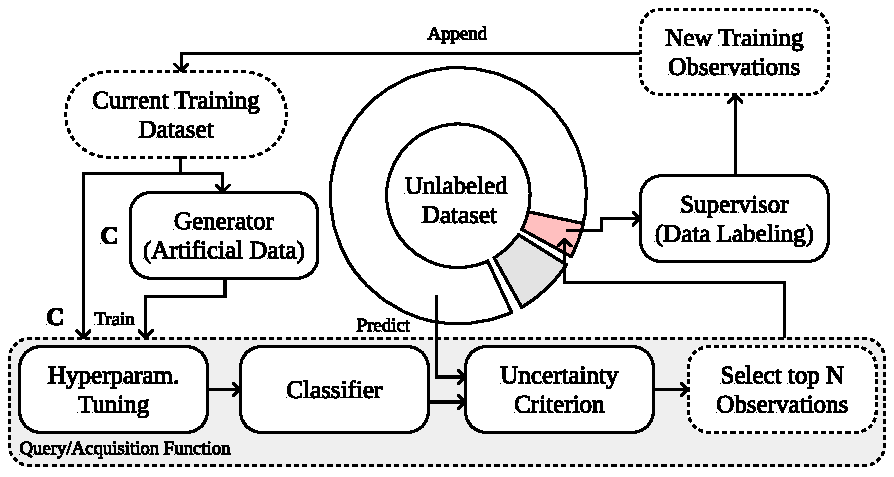
\includegraphics[width=.6\linewidth]{al_proposed}
    \caption{%
        Diagram depicting the proposed AL iteration. The proposed
        modifications are comprised within the red polygon and marked
        with a boldface ``C.''
    }~\label{fig:al_proposed}
\end{figure}

We implemented a simple modification in the selection mechanism of the G-SMOTE
algorithm to show the effectiveness of data augmentation in an AL
implementation. We use the uncertainties produced by $f_{acq}$ to compute the
probabilities of observations to be selected for augmentation as an additional
parameter. This modification is described in Algorithm~\ref{alg:g-smote} 

\begin{algorithm}[ht]
    \SetKwInput{KwGiven}{Given}
    \SetKwProg{Fn}{Function}{:}{end}
    \caption{Proposed AL Framework (Single iteration)}\label{alg:al-framework}
    \DontPrintSemicolon%
    \KwGiven{$t \ge 1$, performance metric $f_{pm}$}
    \KwIn{$\mathcal{D}_{pool}$, $\mathcal{D}_{lab}$, $f_c$, $f_{aug}$,
    $f_{acq}$, $\tau_{grid}$, $k$, $n$}
    \KwOut{$\mathcal{D}_{pool}$, $\mathcal{D}_{lab}$}

    \Fn{ParameterTuning($f_c$, $f_{aug}$, $\tau_{grid}$, $\mathcal{D}_{lab}$,
    $k$)}{
        $p \leftarrow 0$ \\
        $\tau \leftarrow \emptyset$ \\
        $\{\mathcal{D}_{lab}^1, \ldots \mathcal{D}_{lab}^k\} \leftarrow
        \mathcal{D}_{lab}$
        \tcp*[f]{$\mathcal{D}_{lab}^n \cap \mathcal{D}_{lab}^m = \emptyset,
        \forall (n, m) \in {1, \ldots, k}$} \\
        \ForAll{$\tau' \in \tau_{grid}$}{
            $p' \leftarrow \emptyset$ \\
            \ForAll{
                $\mathcal{D}_{lab}^i \in \{\mathcal{D}_{lab}^1, \ldots
                \mathcal{D}_{lab}^k\}$
            }{
                $\mathcal{D}_{test}' \leftarrow \mathcal{D}_{lab}^i$ \\
                $\mathcal{D}_{train}' \leftarrow \mathcal{D}_{lab} \setminus
                \mathcal{D}_{lab}^i$ \\
                $\mathcal{D}_{train}' \leftarrow f_{aug}(\mathcal{D}_{train}';
                \tau')$ \\
                \textbf{train} $f_c$ using $\mathcal{D}_{train}'$ \\
                $p' \leftarrow p' \cup \{f_{pm}(f_c(\mathcal{D}_{test}))\}$
            }
            $p' \leftarrow \frac{\sum_{x_i \in p'}{x_i}}{k}$ \\
            \If{$p' > p$}{
                $p \leftarrow p'$ \\
                $\tau \leftarrow \tau'$
            }
        }
        \Return $\tau$
    }

    \Begin{
        $\tau \leftarrow ParameterTuning(f_c, f_{aug}, \tau_{grid},
        \mathcal{D}_{lab}, k)$ \\
        $\mathcal{D}_{train} \leftarrow f_{aug}(\mathcal{D}_{lab}; \tau)$ \\
        \textbf{train} $f_c$ using $\mathcal{D}_{train}$ \\
        $\mathcal{D}_{new} = \arg\max_{\mathcal{D}_{pool}'\subset
        \mathcal{D}_{pool}, |\mathcal{D}_{pool}'|=n} \sum_{x \in
        \mathcal{D}_{pool}'}{f_{acq}(x; f_c)}$ \\
        \textbf{annotate} $\mathcal{D}_{new}$ \\
        $\mathcal{D}_{pool} \leftarrow \mathcal{D}_{pool} \setminus
        \mathcal{D}_{new}$ \\
        $\mathcal{D}_{lab} \leftarrow \mathcal{D}_{lab} \cup
        \mathcal{D}_{new}$ \\
    }

\end{algorithm}

This modification facilitates the usage of G-SMOTE beyond its original
oversampling purposes. However, in this paper, the data augmentation
strategies are also used to ensure that class frequencies are balanced.
Furthermore, the amount of artificial data produced for each class is defined
by the \textit{augmentation factor}, $\alpha_{af}$, which represents a
percentage of the majority class $C_{maj}$ (\textit{e.g.,} an augmentation
factor of $1.2$ will ensure there are $count(C_{maj}) \times 1.2$ observations
in every class). In this paper's experiment, the data generation mechanism is
similar to the one in~\cite{Fonseca2021al}. This factor allows the direct
comparison of the two frameworks and establishes a causality of the
performance variations to the data generation mechanism (\textit{i.e.,}
augmentation vs normal oversampling) and hyperparameter tuning steps.
However, in this case, the hyperparameter tuning is solely going to be used
for augmentation policy optimization. 

\begin{algorithm}[t]
    \SetKwInput{KwGiven}{Given}
    \SetKwProg{Fn}{Function}{:}{end}
    \caption{G-SMOTE Modified for Data Augmentation in AL}\label{alg:g-smote}
    \DontPrintSemicolon% 
    \KwGiven{$t \ge 1$, $\mathcal{D}_{lab}^t \ne \emptyset$,
    $\mathcal{D}_{lab} = \mathcal{D}_{lab}^{min} \cup \mathcal{D}_{lab}^{maj}$, \textit{GSMOTE}}
    \KwIn{$\mathcal{D}_{pool}^t$, $\mathcal{D}_{lab}^t$, $f_c^{t-1}$,
    $f_{acq}$, $\tau$}
    \KwOut{$\mathcal{D}_{train}^t$}

    \Fn{DataSelection($\mathcal{D}_{lab}^t$, $f_{acq}$, $f_c^{t-1}$)}{%
        $U \leftarrow \emptyset$ \\ 
        $P \leftarrow \emptyset$ \\ 
        $p_s \sim \mathcal{U}(0, 1)$ \\
        \ForAll{$x_i \in \mathcal{D}_{lab}^t$}{
            $u_{x_i} \leftarrow f_{acq}(x_i; f_c^{t-1})$\\
            $U \leftarrow U \cup \{u_{x_i}\}$
        }
        \ForAll{$u_{x_i} \in U$}{
            $p_{x_i} \leftarrow \frac{u_{x_i}}{\sum{U}} + \sum{P}$ \\
            $P \leftarrow P \cup \{p_{x_i}\}$
        }
        $i \leftarrow argmax(P < p_s)$ \\
        \Return i-th element in $\mathcal{D}_{lab}^t$
    }
    \Begin{
        $\mathcal{D}_{aug}^{min} \leftarrow \emptyset$ \\
        $\mathcal{D}_{aug}^{maj} \leftarrow \emptyset$ \\
        $\alpha_{af}, \alpha_{trunc}, \alpha_{def} \leftarrow \tau$ \\
        $N \leftarrow count(C_{maj}) \times \alpha_{af}$ \\
        
        \ForAll{
            $\mathcal{D}'_{aug} \in \{\mathcal{D}_{aug}^{min},
            \mathcal{D}_{aug}^{maj}\}$, $\mathcal{D}'_{lab} \in \{\mathcal{D}_{lab}^{min},
            \mathcal{D}_{lab}^{maj}\}$
        }{
            \While{
                $|\mathcal{D}'_{aug}| < N$
            }{
                $x_{center} \leftarrow DataSelection(\mathcal{D}'_{lab},
                f_{acq}, f_c^{t-1})$ \\
                $x_{gen} \leftarrow GSMOTE(x_{center}, \mathcal{D}_{lab}^t, \alpha_{trunc},
                \alpha_{def})$ \\
                $\mathcal{D}'_{aug} \leftarrow \mathcal{D}'_{aug} \cup
                \{x_{gen}\}$
            }
        }
        $\mathcal{D}_{aug} \leftarrow \mathcal{D}_{aug}^{min} \cup \mathcal{D}_{aug}^{maj}$ \\
        $\mathcal{D}_{train}^t \leftarrow \mathcal{D}_{lab}^t \cup
        \mathcal{D}_{aug}$
    }
\end{algorithm}

In the proposed framework, we (1) generalize the generator module to accept
any data augmentation method or policy and (2) introduce a hyperparameter
tuning module to estimate the optimal data augmentation policy. This framework
was designed to be task-agnostic. Specifically, any data augmentation method
(domain-specific or not) may be applied, as well as any other parameter search
method. It is also expected to be compatible with other AL modifications,
including those that do not affect solely the classifier or uncertainty
criterion, such as the one proposed in~\cite{Yoo2019}.
 
\section{Methodology}~\label{sec:methodology-al-aug}

This section describes the different elements included in the experimental
procedure. The datasets used were acquired in open data repositories. Their
sources and preprocessing steps are defined in
Subsection~\ref{sec:datasets-al-aug}.
The classifiers used in the experiment are defined in
Subsection~\ref{sec:machine_learning_algorithms-al-aug}. The metrics chosen to
measure AL performance and overall classification performance are defined in
Subsection~\ref{sec:evaluation_metrics-al-aug}. The experimental procedure is
described in Subsection~\ref{sec:experimental_procedure-al-aug}.

The methodology developed serves a two-fold purpose: (1) Compare
classification performance once all the AL procedures are completed
(\textit{i.e.,} optimal performance of a classifier trained via iterative data
selection) and (2) Compare the amount of data required to reach specific
performance thresholds (\textit{i.e.,} the number of AL iterations required to
reach similar classification performances).
 
\subsection{Datasets}~\label{sec:datasets-al-aug}

The datasets used to test the proposed method are publicly available in open
data repositories. Specifically, they were retrieved from the OpenML and the
UCI Machine Learning Repository websites. They were chosen considering diverse
application domains, imbalance ratios, dimensionality and number of target
classes, all of them focused on classification tasks. The goal is to
demonstrate the performance of the different AL frameworks in various
scenarios and domains. The data preprocessing approach was similar across all
datasets.  Table~\ref{tab:datasets_description} describes the key properties
of the 15 preprocessed datasets where the experimental procedure was applied. 
 
\begin{table}
    \centering
    \setlength{\tabcolsep}{2pt}
    \caption{\label{tab:datasets_description}
        Description of the datasets collected after data preprocessing. The
        sampling strategy is similar across datasets. Legend: (IR) Imbalance
        Ratio
    }
    \pgfplotstabletypeset[
        col sep=comma,
        string type,
        every head row/.style={%
            before row=\toprule,
            after row=\midrule
        },
        every last row/.style={after row=\bottomrule},
    ]{figures/active-learning-augmentation/datasets_description.csv}
\end{table}

The data preprocessing pipeline is depicted as a flowchart in
Figure~\ref{fig:data_preprocessing}. The missing values are removed from each
dataset by removing the corresponding observations. This step ensures that the
input data in the experiment is kept as close to its original form as
possible. The non-metric features (\textit{i.e.,} binary, categorical, and
ordinal variables) were removed since the application of G-SMOTE is limited to
continuous and discrete features. The datasets containing over 2000
observations were downsampled in order to maintain the datasets to a
manageable size. The data sampling procedure preserves the relative class
frequency of the dataset, in order to maintain the Imbalance Ratio (IR)
originally found in each dataset (where $IR =
\frac{count(C_{maj})}{count(C_{\min})}$). The remaining features of each
dataset are scaled to the range of $[-1, 1]$ to ensure a common range across
features.

\begin{figure}[t]
	\centering
	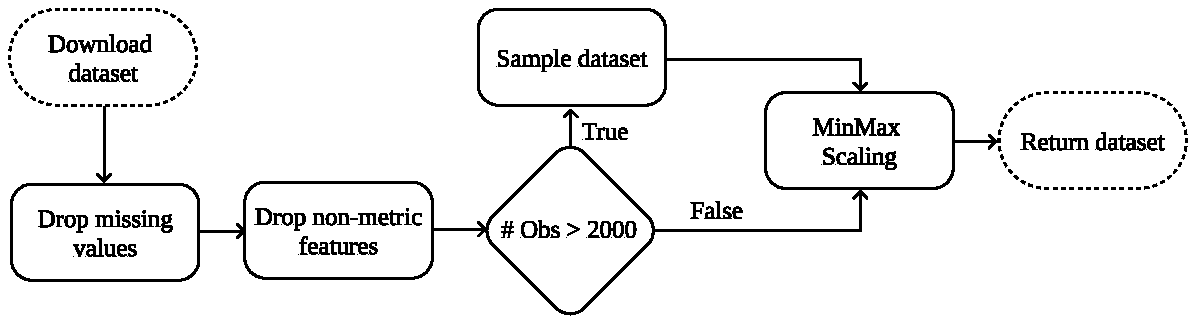
\includegraphics[width=.8\linewidth]{data_preprocessing}
    \caption{%
        Data preprocessing pipeline.
    }~\label{fig:data_preprocessing}
\end{figure}

The preprocessed datasets were stored into an SQLite database file and is
available along with the experiment's source code in the project's GitHub
repository (see final remarks regarding data and software availability).
 
\subsection{Machine Learning Algorithms}~\label{sec:machine_learning_algorithms-al-aug}

We used a total of four classification algorithms and a heuristic data
augmentation mechanism. The choice of classifiers was based on the popularity
and family of the classifiers (tree-based, nearest neighbors-based,
ensemble-based and linear models). Our proposed method was tested using a
Decision Tree (DT)~\cite{Wu1975}, a K-nearest neighbors classifier
(KNN)~\cite{Cover1967}, a Random Forest Classifier (RF)~\cite{Ho1995} and a
Logistic Regression (LR)~\cite{Nelder1972}. Since the target variables are
multi-class, the LR classifier was implemented using the one-versus-all
approach. The predicted class is assigned to the label with the highest
likelihood.
 
The oversampler G-SMOTE was used as a data augmentation method. The typical
data generation policy of oversampling methods is to generate artificial
observations on non-majority classes such that the number of majority class
observations matches those of each non-majority class. We modified this data
generation policy to generate observations for all classes, as a percentage of
the number of observations in the majority class. In addition, the original
G-SMOTE algorithm was modified to accept data selection probabilities based on
classification uncertainty. These modifications are discussed in
Section~\ref{sec:proposed_method-al-aug}.

Every AL procedure was tested with different selection criteria: Random
Selection, Entropy, and Breaking Ties. The baseline used is the standard AL
procedure. As a benchmark, we add the AL procedure using G-SMOTE as a standard
oversampling method, as proposed in~\cite{Fonseca2021al}. Our proposed method
was implemented using G-SMOTE as a data augmentation method to generate
artificial observations for all classes, while still balancing the class
distribution, as described in Section~\ref{sec:proposed_method-al-aug}. 
 
\subsection{Evaluation Metrics}~\label{sec:evaluation_metrics-al-aug}

Considering the imbalanced nature of the datasets used in the experiment,
commonly used performance metrics such as Overall Accuracy (OA), although
being intuitive to interpret, are insufficient to quantify a model's
classification performance~\cite{Jeni2013}. The Cohen's Kappa performance
metric, similar to OA, is also biased towards high-frequency classes since its
definition is closely related to the OA metric, making its behavior consistent
with OA~\cite{Fatourechi2008}. However, these metrics remain popular choices
for the evaluation of classification performance. Other performance metrics
like $Precision = \frac{TP}{TP+FP}$, $Recall = \frac{TP}{TP+FN}$ (also
known as Sensitivity) or $Specificity = \frac{TN}{TN + FP}$ are calculated as
a function of True/False Positives (TP and FP) and True/False Negatives (TN
and FN) and can be used on a per-class basis instead. In a multiple dataset
scenario with varying amounts of target classes and meanings, comparing the
performance of different models using these metrics becomes impractical.
 
Based on the recommendations found in~\cite{Jeni2013, Kubat1997}, we used two
metrics found to be less sensitive to the class imbalance bias, along with OA
as a reference for easier interpretability:

\begin{itemize}
    \item The Geometric-mean scorer (G-mean) consists of the geometric mean of
        Specificity and Recall~\cite{Kubat1997}. Both metrics are calculated
        in a multi-class context considering a one-versus-all approach. For
        multi-class problems, the G-mean scorer is calculated as its average
        per class values: 
        
        \begin{equation*}
            \textit{G-mean} = \sqrt{\overline{Recall} \times
            \overline{Specificity}}
        \end{equation*}

    \item The F-score metric consists of the harmonic mean of Precision and
        Recall. The two metrics are also calculated considering a
        one-versus-all approach. The F-score for the multi-class case can be
        calculated using its average per class values~\cite{Jeni2013}:

        \begin{equation*}
            \textit{F-score}=2\times\frac{\overline{Precision} \times
            \overline{Recall}}{\overline{Precision} + \overline{Recall}}
        \end{equation*}

    \item The OA consists of the number of TP divided by the total amount of
        observations. Considering $c$ as the label for the different classes
        present in a target class, OA is given by the following formula:

        \begin{equation*}
            \textit{OA} = \frac{\sum\limits_{c}{\text{TP}_{c}}}{%
		    	      \sum\limits_{c}{(\text{TP}_{c}+\text{FP}_{c})}}
        \end{equation*}
\end{itemize}

The comparison of the performance of AL frameworks is based on its data
selection and augmentation efficacy. Specifically, an efficient data
selection/generation policy allows the production of classifiers with high
performance on unseen data while using as least non-artificial training data
as possible. We follow the recommendations found in~\cite{Kottke2017}. To
measure the performance of the different AL setups, the performance of an AL
setup will be compared using two AL-specific performance metrics:

\begin{itemize}

    \item Area Under the Learning Curve (AULC). It is the sum of the
        classification performance over a validation/test set of the
        classifiers trained of all AL iterations. The resulting AULC scores
        are fixed within the range $[0, 1]$ by dividing the AULC scores by the
        total amount of iterations (\textit{i.e.}, the maximum performance
        area) to facilitate the interpretability of this metric.

    \item Data Utilization Rate (DUR)~\cite{Reitmaier2013}. Measures the
        percentage of training data required to reach a given performance
        threshold, as a ratio of the percentage of training data required by
        the baseline framework. This metric is also presented as a percentage
        of the total amount of training data, without making it relative to
        the baseline framework. The DUR metric is measured at 45 different
        performance thresholds, ranging between $[0.10, 1.00]$ at a 0.02 step.

\end{itemize}
 
\subsection{Experimental Procedure}~\label{sec:experimental_procedure-al-aug}

The evaluation of different active learners in a live setting is generally
expensive, time-consuming, and prone to human error. Instead, a common
practice is to compare them in an offline environment using labeled
datasets~\cite{Kagy2019}. Since the dataset is already labeled, the annotation
process is done at zero cost in this scenario.
Figure~\ref{fig:experimental_procedure} depicts the experiment designed for
one dataset over a single run. 
 
A single run starts with the splitting of a preprocessed dataset into five
different partitions, stratified according to the class frequencies of the
target variable using the K-fold Cross Validation method. During this run, an
active learner or classifier is trained five times using a different partition
as the Test set each time. For each training process, a validation set
containing 25\% of the subset is created and is used to measure the data
selection efficiency (\textit{i.e.,} AULC and DUR using the classification
performance metrics, specific to AL). Therefore, for a single training
procedure, 20\% of the original dataset is used as the validation set, 20\% is
used as the Test set and 60\% is used as the training set. The AL simulations
and the classifiers' training occur within the training set. However, the
classifiers used to find the maximum performance classification scores are
trained over the full training set. The AL simulations are run over a maximum
of 50 iterations (including the initialization step), adding 1.6\% of the
training set each time (\textit{i.e.,} all AL simulations use less than 80\%
of the training set). Once the training phase is completed, the Test set
classification scores are calculated using the trained classifiers. For the
case of AL, the classifier with the optimal validation set score is used to
estimate the AL's optimal classification performance over unseen data.

The process shown in Figure~\ref{fig:experimental_procedure} is repeated over
three runs using different random seeds over the 15 different datasets
collected. The final scores of each AL configuration and classifier correspond
to the average of the three runs and 5-fold Cross-Validation estimations
(\textit{i.e.,} the mean score of 15 fits, across 15 datasets).

\begin{figure}
	\centering
	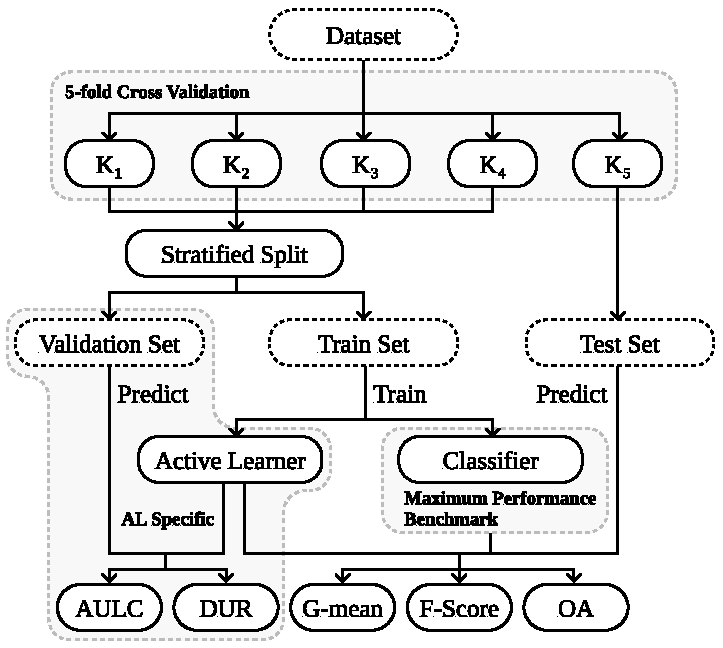
\includegraphics[width=.6\linewidth]{experimental_procedure}
    \caption{%
        Experimental procedure flowchart. The preprocessed datasets are split
        into five folds. One of the folds is used to test the best-found
        classifiers using AL and the classifiers trained using the entire
        training dataset (containing the remaining folds). The training set is
        used to run both the AL simulations as well as train the normal
        classifiers. The validation set is used to measure AL-specific
        performance metrics over each iteration. We use different subsets for
        overall classification performance and AL-specific performance to
        avoid data leakage.
    }~\label{fig:experimental_procedure}
\end{figure}

The hyperparameters defined for the AL frameworks, Classifiers, and Generators
are shown in Table~\ref{tab:grid}. In the Generators table, we distinguish the
G-SMOTE algorithm working as a normal oversampling method from G-SMOTE-AUGM,
which generates additional artificial data on top of the usual oversampling
mechanism. Since the G-SMOTE-AUGM method is intended to be used with varying
parameter values (via within-iteration parameter tuning), the parameters were
defined as a list of various possible values. The remaining parameters
were selected based on knowledge gathered in previous literature and
typical default values for each of the algorithms. This choice was motivated
by the impossibility of parameter tuning in a real-world setting when applying
the benchmark AL methods. Although the proposed method addresses this
limitation, we show that exclusively tuning the parameters on the augmentation
policy is already sufficient to achieve superior, statistically significant
performance.

\begin{table}
	\centering
    \caption{\label{tab:grid}
        Hyperparameter definition for the active learners, classifiers,
        and generators used in the experiment.
    }
	\begin{tabular}{lll}
		\toprule
		Active Learners & Hyperparameters                   & Inputs                         \\
		\midrule
		Standard        & \# initial obs.\                  & 1.6\%                          \\
                        & \# additional obs.\ per iteration & 1.6\%                          \\
                        & max.\ iterations + initialization & 50                             \\
                        & evaluation metrics                & G-mean, F-score, OA            \\
                        & selection strategy                & Random, Entropy, Breaking Ties \\
                        & within-iteration param.\ tuning   & None                           \\
                        & generator                         & None                           \\
                        & classifier                        & DT, LR, KNN, RF                \\
        Oversampling    & generator                         & G-SMOTE                        \\
        Proposed        & generator                         & G-SMOTE-AUGM                   \\
                        & within-iteration param.\ tuning   & Grid Search K-fold CV          \\
		\toprule
		Classifier      &                                  &                                \\
		\midrule
        DT              & min.\ samples split              & 2                              \\
                        & criterion                        & gini                           \\
		LR              & maximum iterations               & 100                            \\
                        & multi-class                      & One-vs-All                     \\
		                & solver                           & liblinear                      \\
                        & penalty                          & L2 (Ridge)                     \\
		KNN             & \# neighbors                     & 5                              \\
                        & weights                          & uniform                        \\
                        & metric                           & euclidean                      \\
		RF              & min.\ samples split              & 2                              \\
		                & \# estimators                    & 100                            \\
                        & criterion                        & gini                           \\
		\toprule
		Generator       &                                  &                                \\
		\midrule
		G-SMOTE         & \# neighbors                     & 4                              \\
                        & deformation factor               & 0.5                            \\
                        & truncation factor                & 0.5                            \\
		G-SMOTE-AUGM    & \# neighbors                     & 3, 4, 5                        \\
                        & deformation factor               & 0.5                            \\
                        & truncation factor                & 0.5                            \\
                        & augmentation factor              & $[1.1, 2.0]$ at 0.1 step       \\
		\bottomrule
	\end{tabular}
\end{table}
 
\subsection{Software Implementation}~\label{sec:software_implementation}

The experiment was implemented using the Python programming language, along
with the Python libraries
\href{https://scikit-learn.org/stable/}{Scikit-Learn}~\cite{Pedregosa2011},
\href{https://imbalanced-learn.org/en/stable/}{Imbalanced-Learn}~\cite{JMLR:v18:16-365},
\href{https://geometric-smote.readthedocs.io/en/latest/?badge=latest}{Geometric-SMOTE}~\cite{Douzas2019},
\href{https://research-learn.readthedocs.io/en/latest/?badge=latest}{Research-Learn}
and
\href{https://mlresearch.readthedocs.io/en/latest/?badge=latest}{ML-Research}
libraries. All functions, algorithms, experiments, and results are provided in
the \href{https://github.com/joaopfonseca/publications/}{project's GitHub
repository}. The original datasets used in this study are publicly available
in open data repositories. They were retrieved from OpenML and the UCI Machine
Learning Repository. 

\section{Results \& Discussion}~\label{sec:results_discussion-al-aug}

In a multiple dataset experiment, the analysis of results should not rely upon
the average performance scores across datasets uniquely. The domain of
application and fluctuations of performance scores between datasets make the
analysis of these averaged results less accurate. Instead, it is generally
recommended to use the mean ranking scores to extend the
analysis~\cite{Demsar2006}. Since mean performance scores are still intuitive
to interpret; we will present and discuss both results. The rank values are
assigned based on the mean scores of three different 5-fold Cross-Validation
runs (15 performance estimations per dataset) for each combination of dataset,
AL configuration, classifier, and performance metric.
 
\subsection{Results}~\label{sec:results-al-aug}

The average rankings of the AL methods' AULC estimations are shown in
Table~\ref{tab:aulc_ranks}. The proposed method almost always improves AL
performance and ensures higher data selection efficiency.
 
\begin{table}[ht]
	\centering
    \caption{%
        Mean rankings of the AULC metric over the different datasets (15),
        folds (5), and runs (3) used in the experiment. The proposed method
        constantly improves the results of the original framework and, on
        average, almost always improves the results of the oversampling
        framework.
    }\label{tab:aulc_ranks}
    \pgfplotstabletypeset[
        col sep=comma,
        string type,
        every head row/.style={%
            before row=\toprule,
            after row=\midrule
        },
        every last row/.style={after row=\bottomrule},
    ]{figures/active-learning-augmentation/mean_std_aulc_ranks.csv}
\end{table}
 
Table~\ref{tab:aulc_scores} shows the average AULC scores, grouped by the
classifier, Evaluation Metric and AL framework. The performance of the
proposed method is almost always superior when considering the F-score and
G-mean. On some occasions, the average AULC score is significantly improved
when compared with the oversampling AL method.

\begin{table}
	\centering
    \setlength{\tabcolsep}{2.5pt}
    \caption{\label{tab:aulc_scores}
        Average AULC of each AL configuration tested. Each AULC score is
        calculated using the performance scores of each iteration in the
        validation set. By the end of the iterative process, each AL
        configuration used a maximum of 80\% instances of the 60\% instances
        that compose the training sets (\textit{i.e.,} 48\% of the entire
        preprocessed dataset).
    }
    \pgfplotstabletypeset[
        col sep=comma,
        string type,
        every head row/.style={%
            before row=\toprule,
            after row=\midrule
        },
        every last row/.style={after row=\bottomrule},
    ]{figures/active-learning-augmentation/mean_std_aulc_scores.csv}
\end{table}

The average DUR scores were calculated for various G-mean thresholds, varying
between 0.1 and 1.0 at a 0.02 step (45 different thresholds in total).
Table~\ref{tab:optimal_data_utilization} shows the results obtained for these
scores starting from a G-mean score of 0.6 and was filtered to show the
thresholds ending with 0 or 6 only. In most cases, the proposed method reduces
the amount of data annotation required to reach each G-mean score threshold.

\begin{table}[t]
    \centering
    \setlength{\tabcolsep}{2.5pt}
    \caption{\label{tab:optimal_data_utilization}
        AL algorithms' mean data utilization as a percentage of the
        training set.
    }
    \pgfplotstabletypeset[
        col sep=comma,
        string type,
        every head row/.style={%
            before row=\toprule,
            after row=\midrule
        },
        every last row/.style={after row=\bottomrule},
    ]{figures/active-learning-augmentation/optimal_data_utilization.csv}
\end{table}

The DUR scores relative to the Standard AL method are shown in
Figure~\ref{fig:dur}. A DUR below 1 means that the Proposed/Oversampling
method requires less data than the Standard AL method to reach the same
performance threshold. For example, running an AL simulation using the KNN
classifier requires 80.7\% of the amount of data required by the Standard AL
method using the same classifier to reach an F-Score of 0.62 (\textit{i.e.,}
requires 19.3\% less data).

\begin{figure}[t]
	\centering
	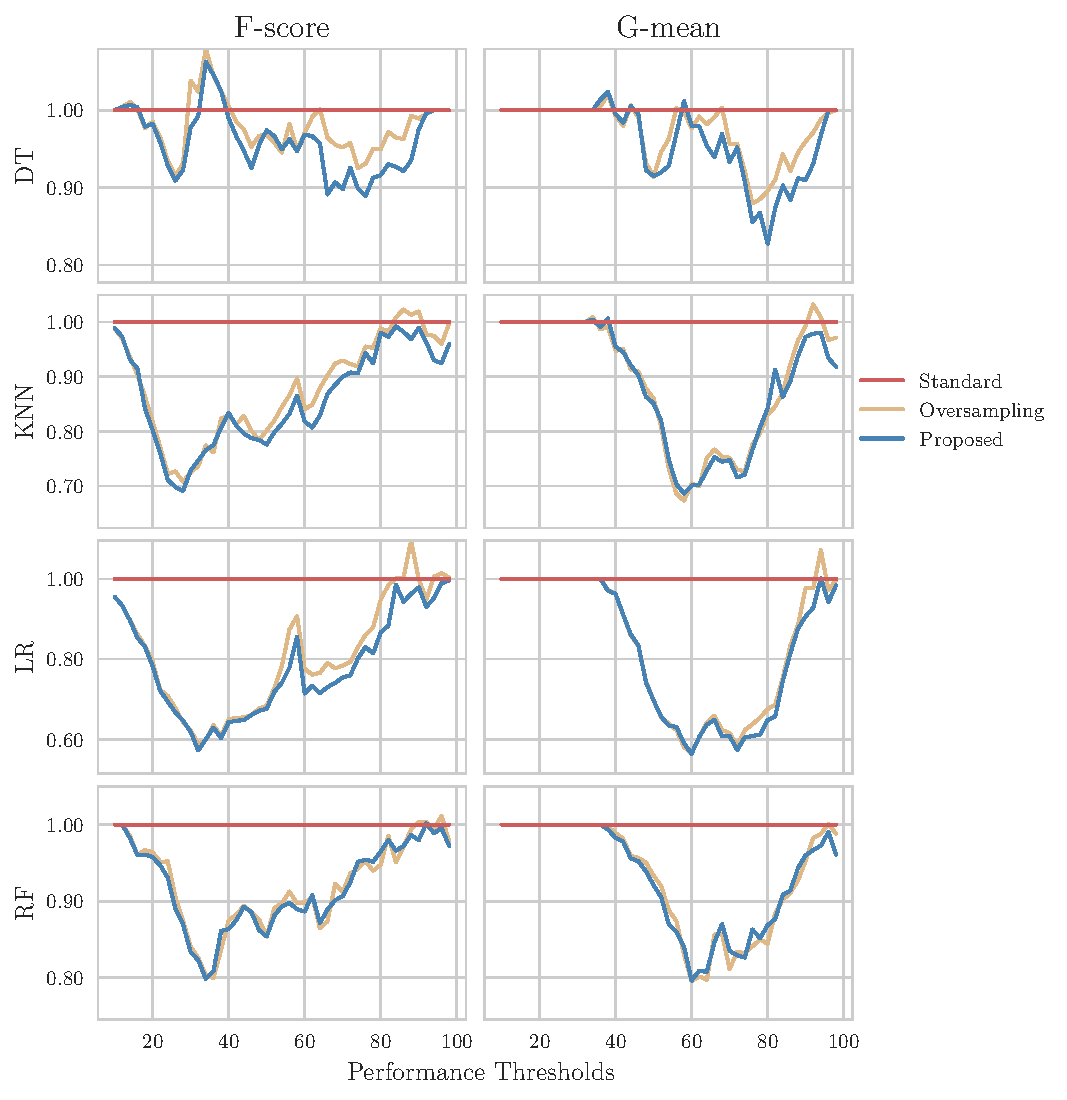
\includegraphics[width=.8\linewidth]{data_utilization_rate}
    \caption{%
        Mean data utilization rates. The y-axis shows the percentage of data
        (relative to the baseline AL framework) required to reach the
        different performance thresholds.
    }~\label{fig:dur}
\end{figure}

The comparison of mean optimal classification scores of AL methods with
Classifiers (using the entire training set, without AL) is shown in
Table~\ref{tab:optimal_mean_std_scores}. Aside from the case of overall
accuracy, the proposed AL method produces classifiers that almost consistently
outperform classifiers using the whole training set (\textit{i.e.,} the ones
labeled as MP).

\begin{table}
    \centering
    \caption{\label{tab:optimal_mean_std_scores}
        Optimal classification scores. The Maximum Performance (MP)
        classification scores are calculated using classifiers trained using
        the entire training set.
    }
    \pgfplotstabletypeset[
        col sep=comma,
        string type,
        every head row/.style={%
            before row=\toprule,
            after row=\midrule
        },
        every last row/.style={after row=\bottomrule},
    ]{figures/active-learning-augmentation/optimal_mean_std_scores.csv}
\end{table}

\subsection{Statistical Analysis}~\label{sec:statistical-analysis-al-aug}

When checking for statistical significance in a multiple dataset context it is
critical to account for the multiple comparison problem. Consequently, our
statistical analysis focuses on the recommendations found
in~\cite{Demsar2006}. Overall, we perform three statistical tests. The
Friedman test~\cite{Friedman1937} is used to understand whether there is a
statistically significant difference in performance between the three AL
frameworks. As \textit{post hoc} analysis, the Wilcoxon signed-rank
test~\cite{Wilcoxon1945} was utilized to check for statistical significance
between the performance of the proposed AL method and the oversampling AL
method across datasets. As a second \textit{post hoc} analysis, the
Holm-Bonferroni~\cite{Holm1979} method was employed to check for statistical
significance between the methods using data generators and the Standard AL
framework across classifiers and evaluation metrics.
 
Table~\ref{tab:friedman_test} displays the \textit{p-values} obtained with the
Friedman test. The difference in performance across AL frameworks is
statistically significant at a level of $\alpha = 0.05$ regardless of the
classifier or evaluation metric being considered.

\begin{table}[t]
	\centering
    \caption{%
        Friedman test results. Statistical significance is tested at a level
        of $\alpha = 0.05$. The null hypothesis is that there is no difference
        in the classification outcome across oversamplers.
    }\label{tab:friedman_test}
    \pgfplotstabletypeset[
        col sep=comma,
        string type,
        every head row/.style={%
            before row=\toprule,
            after row=\midrule
        },
        every last row/.style={after row=\bottomrule},
    ]{figures/active-learning-augmentation/friedman_test.csv}
\end{table}

Table~\ref{tab:wilcoxon_test_al_aug} contains the \textit{p-values} obtained with the
Wilcoxon signed-rank test. The proposed method was able to outperform both the
standard AL framework, as well as the AL framework using a typical
oversampling policy with statistical significance in 14 and 12 out of 15
datasets, respectively.

\begin{table}
	\centering
    \caption{%
        Adjusted p-values using the Wilcoxon signed-rank method. Bold values
        are statistically significant at a level of $\alpha = 0.05$. The null
        hypothesis is that the performance of the proposed framework is
        similar to that of the oversampling or standard framework.
    }\label{tab:wilcoxon_test_al_aug}
    \pgfplotstabletypeset[
        col sep=comma,
        string type,
        every head row/.style={%
            before row=\toprule,
            after row=\midrule
        },
        every last row/.style={after row=\bottomrule},
    ]{figures/active-learning-augmentation/wilcoxon_test.csv}
\end{table}

The \textit{p-values} shown in Table~\ref{tab:holms_test} refer to the results
of the Holm-Bonferroni test. The proposed method's superior performance was
statistically significant in 9 out of 12 cases. 

\begin{table}
	\centering
    \caption{%
        Adjusted p-values using the Holm-Bonferroni method. Bold values are
        statistically significant at a level of $\alpha = 0.05$. The null
        hypothesis is that the Oversampling or Proposed method does not
        perform better than the control method (Standard AL framework).
    }\label{tab:holms_test}
    \pgfplotstabletypeset[
        col sep=comma,
        string type,
        every head row/.style={%
            before row=\toprule,
            after row=\midrule
        },
        every last row/.style={after row=\bottomrule},
    ]{figures/active-learning-augmentation/holms_test.csv}
\end{table}

\subsection{Discussion}~\label{sec:sub_discussion-al-aug}

In this paper, we study the application of data augmentation methods through
the modification of the standard AL framework. This is done to further reduce
the amount of labeled data required to produce a reliable classifier, at the
expense of artificial data generation. Overall, the proposed method
achieves better and more consistent performance when compared to the remaining
benchmark approaches. It was implemented to focus on the optimization of the
data augmentation policy, as well as the introduction of a more informed
AL-based data augmentation approach. The proposed method could be further
extended and achieve an even higher performance by optimizing parameters of
the ML classification using the hyperparameter optimizer. In addition, this
framework could be further generalized by searching, within AL iterations, for
the optimal ML classifier as well; at different stages of the data collection
procedure some ML classifiers might be more useful than others. Although the
proposed framework significantly improves the flexibility of AL
implementations, we found that even a superficial parameter search is
sufficient to ensure a superior performance when compared to related
approaches.
 
% a different data generation strategy
% - Superiority of AL proposed vs standard (AULC + statistical analysis)
In Table~\ref{tab:aulc_ranks}, we found that the proposed method was able to
outperform the Standard AL framework in all scenarios. Except for the overall
accuracy metric, the mean rankings are consistent with the mean AULC scores
found in Table~\ref{tab:aulc_scores}, while showing performance improvements
between the proposed method and both the standard and oversampling methods.
The Friedman test in Table~\ref{tab:friedman_test} showed that the difference
in the performance of these AL frameworks are statistically significant,
regardless of the classifier or performance metric being used.
 
% parameter optimization within the iterative process of an AL procedure
% - Discuss consistency of results as compared with other methods (DUR metric)
The proposed method evidenced more consistent data utilization requirements in
most of the assessed G-mean score thresholds when compared to the remaining AL
methods, as seen in Table~\ref{tab:optimal_data_utilization}. For example, to
reach a G-mean score of 0.9 using the KNN and LR classifiers, the average
amount of data required with the Oversampling AL approach increased when
compared to the standard approach. However, the proposed method was able to
decrease the amount of data required in both situations. The robustness of the
proposed method is clearer in Figure~\ref{fig:dur}. In most cases, this method
was able to outperform the Oversampling method. At the same time, the proposed
method also addresses inconsistencies in situations where the Oversampling
method was unable to outperform the standard method.

% Data augmentation vs oversampling
The statistical analyses found in Tables~\ref{tab:wilcoxon_test_al_aug}
and~\ref{tab:holms_test} revealed that the proposed method's superiority was
statistically significant in all datasets except three (Baseball, Usps, and
Volkert) and established statistical significance when compared to the
standard AL method for all combinations of classifier and performance metric,
except for three cases regarding the use of the overall accuracy metric. These
results show that the proposed method increased the reliability of the new AL
framework and improved the quality of the final classifier while using fewer
data.

% Usage of AL as a method to produce better performing classifiers, even in
% settings with fully labeled data
Even though it was not the core purpose of this study, we found that the
proposed AL method consistently outperformed the maximum performance
threshold. Specifically, in Table~\ref{tab:optimal_mean_std_scores}, the
performance of the classifiers originating from the proposed method was able
to outperform classifiers trained using the full training dataset in 9 out of
12 scenarios. This outcome suggests that the selection of a meaningful
training subset training dataset paired with data augmentation not only
matches the classification performance of ML algorithms, as it also improves
them. Even in a setting with fully labeled training data, the proposed method
may be used as a preprocessing technique to further optimize classification
performance.

% Future work and limitations
This study discussed the effect of data augmentation within the AL framework,
along with the exploration of optimal augmentation methods within AL
iterations. However, the conceptual nature of this study implies some
limitations. Specifically, the large number of experiments required to
test the method's efficacy, along with the limited computational power
available, led to a limited exploration of the grid search's potential. Future
work should focus on understanding how the usage of a more comprehensive
parameter tuning approach improves the quality of the AL method. In addition,
the proposed method was not able to outperform the standard AL method at
100\% of scenarios. The exploration of other, more complex data augmentation
techniques might further improve its performance by producing more
meaningful training observations. Specifically, in this study, we assume
that all datasets used follow a manifold, allowing the usage of G-SMOTE as a
data augmentation approach. However, this method cannot be used in more
complex, non-euclidean spaces. In this scenario, the usage of G-SMOTE is not
valid and might lead to the production of noisy data. Deep Learning-based data
augmentation techniques are able to address this limitation and improve the
overall quality of the artificial data being generated. We also
encountered significant standard errors throughout our experimental
results (see Subsection~\ref{sec:results-al-aug}), consistent with the findings
in~\cite{Fonseca2021al, Kottke2017}. This facet suggests that the usage of
more robust generators did not decrease the standard error of AL performance.
Instead, AL's performance variability is likely dependent on the quality of
its initialization.

\section{Conclusion and Future Directions}~\label{sec:conclusion-al-aug}

The ability to train ML classifiers is usually limited to the availability of
labeled data. However, manually labeling data is often expensive, which makes
the usage of AL particularly appealing for selecting the most informative
observations and reducing the amount of required labeled data. On the other
hand, the introduction of data variability in the training dataset can also be
conducted via data augmentation. However, most, if not all, AL configurations
that use some form of data augmentation are domain and/or task-specific. These
methods typically apply deep learning approaches to both classification and
data augmentation. Consequently, they may not apply to other classification
tasks or when the available computational power is insufficient.

In this paper, we proposed a domain-agnostic AL framework that implements Data
Augmentation and hyperparameter tuning. We found that a heuristic Data
Augmentation algorithm is sufficient to improve the data selection efficiency
in AL\@. Specifically, the data augmentation method used almost always
increased AL performance, regardless of the target goal (\textit{i.e.,}
optimizing classification or data selection efficiency). The usage of data
augmentation reduced the number of iterations required to train a classifier
with a performance as good as (or better than) classifiers trained with the
entire training dataset (\textit{i.e.,} without using AL). In addition, the
proposed method reduced the size of the training dataset, which is expanded
with artificial data. 

With this revised AL configuration, data selection in AL iterations aims
towards observations that optimize the quality of the artificial data
produced. The substitution of less informative labeled data with artificial
data is especially useful in this context since it reduces some of the user
interaction necessary to reach a sufficiently informative dataset. In order
to further improve the proposed method, future work should (1) focus on the
development of methods with varying data augmentation policies depending on
the different input space regions, (2) develop augmentation-sensitive query
functions capable of avoiding the unnecessary selection of similar
observations from the unlabeled dataset, (3) understand the gap between
randomized data augmentation techniques and neural network/feature
space data augmentation techniques in an AL context better, (4) explore
more efficient ways to leverage the information collected in AL queries for
better augmentation strategies and (5) expand the current framework to
integrate alternative learning strategies using unlabeled data, such as self
and semi supervised learning techniques.

Finally, the proposed method may be applied to any classification problem
where labeled data is not readily available and an easily accessible unlabeled
data pool. For more complex data structures, the application of this framework
will require the learning of a manifold space as an additional preprocessing
step. After that, this AL framework may be used as is.

\chapter{Moving Forward}~\label{chp:moving_forward}

% Focus of chapter 2 and how it links to G-SMOTENC
In Chapter~\ref{chp:data-augmentation-trends} we studied the state-of-the-art
in data augmentation algorithms, which was necessary to proceed to subsequent
steps of the work plan. Based on these findings, in
Chapter~\ref{chp:kmeans-smote} we used an oversampling method to address a
know limitation of imbalanced learning in LULC\@. An additional limitation we
found in oversampling methods was the lack of models capable of addressing
datasets with both metric and non-metric features. We plan to address this
limitation by modifying a state-of-the-art oversampling method, based on RQ4
as described in Subsection~\ref{sec:main_objectives}. This work will be added
as a new Chapter between Chapters~\ref{chp:data-augmentation-trends}
and~\ref{chp:kmeans-smote}.

% Focus of chapter 4 and 5 and how they introduced individual elements to AL,
% the next step is SAD-Learning: merging the different contributions while
% adding other hybrid learning methods to leverage more information from
% unlabeled data
In Chapters~\ref{chp:al-generator-lulc}
and~\ref{chp:active-learning-augmentation} we modify the AL framework as a
means to address RQ3. However, the work presented can be further enriched with
the application of other methods that leverage information from unlabeled
data, specifically semi-supervised and self-supervised learning techniques.
This work is also under development and is intended to follow
Chapter~\ref{chp:active-learning-augmentation}.

The last chapter will close the thesis with the conclusions, discussion of the
proposed research questions and recommendations for future work based on the
results presented in previous chapters.


% REFERENCES
\bibliography{references}
\bibliographystyle{ieeetr}
% \bibliographystyle{plain} % Use to validate duplicate references
\addcontentsline{toc}{part}{Bibliography}


% APPENDICES
\appendix
\cleardoublepage%
\addcontentsline{toc}{part}{Appendices}

\chapter{Improving Imbalanced Land Cover Classification with K-means SMOTE:
Detecting and Oversampling Distinctive Minority Spectral Signatures}

\pgfplotstabletypeset[
	begin table=\begin{longtable},
	end table=\end{longtable},
	col sep=comma,
	header=true,
	columns={Dataset,Classifier,Metric,NONE,ROS,SMOTE,B-SMOTE,K-SMOTE},
    string type,
    every head row/.style={before row={\toprule}, after row=\midrule\endhead},
    every last row/.style={after row={\bottomrule
        \caption[Mean cross-validation scores for each dataset.]{%
            Mean cross-validation scores for each dataset.  Legend: IP -
            Indian Pines, KSC - Kennedy Space Center, PC - Pavia Center, PU -
            Pavia University, SA - Salinas A.
        }~\label{tab:cross_validation_scores}
    }}
]{figures/kmeans-smote-lulc/wide_optimal.csv}

\end{document}
